\documentclass[a4paper,11pt]{book} % Tamaño de papel, tamaño de letra y clase LaTeX usada...

\usepackage[spanish]{babel} % Permite escribir en Castellano (tildes y ñ) e implementa...
\usepackage[utf8]{inputenc} % Permite introducir acentos y Ñ directamente.
%\usepackage[T1]{fontenc} %permite cambiar la fuente por defecto.
\usepackage{bm} % Permite letras griegas en negrita {uso: \bm{\alpha}}
\usepackage{graphicx}
\usepackage{amssymb}
\usepackage{mathtools}
\usepackage{subfigure}
\usepackage{multicol} %para añadir texto en columnas
\usepackage{float}
\usepackage{fancyhdr} %encabezados y pies de pagina
\usepackage{amsmath,amsfonts,latexsym,color,textcomp,anysize}
\usepackage[table,xcdraw]{xcolor}
\usepackage{longtable}
\usepackage{parskip}
\usepackage{hyperref}
\usepackage{cancel} % tachar cosas \cancel{}
% \usepackage{tensor} % Notación: \tensor{T}{^a_b^c_d}
%\usepackage{mathrsfs}
\usepackage{slashed}   %\slashed{p}
\spanishdecimal{.}
\usepackage{cite}
%\usepackage[style=numeric-comp]{biblatex}
\usepackage{yhmath}

\hypersetup{
    colorlinks=true,
    linkcolor=blue,
    filecolor=magenta,      
    urlcolor=cyan}

\usepackage[braket, qm]{qcircuit}

\setcounter{MaxMatrixCols}{12}
\usepackage{changepage}
\usepackage{framed}
\usepackage{caption}
%\usepackage{subcaption}

% Cuadros
\usepackage[most]{tcolorbox}
\tcbuselibrary{listingsutf8}
\newtcolorbox{mybox_blue}[1]
{enhanced jigsaw, breakable, pad at break*=1mm,  colback=cyan!5!white,colframe=cyan!75!black,fonttitle=\bfseries,title=#1}

\newtcolorbox{mybox_green}[1]
{enhanced jigsaw, breakable, pad at break*=1mm, colback=green!5!white,colframe=green!45!black,fonttitle=\bfseries,title=#1}

\newtcolorbox{mybox_red}[1]
{enhanced jigsaw, breakable, pad at break*=1mm, colback=red!5!white,colframe=red!45!black,fonttitle=\bfseries,title=#1}

\newtcolorbox{mybox_orange}[1]
{enhanced jigsaw, breakable, pad at break*=1mm, colback=orange!10!white,colframe=orange!80!black,fonttitle=\bfseries,title=#1}

\newtcolorbox{mybox_gray}[1]
{enhanced jigsaw, breakable, pad at break*=1mm, colframe=gray!45!black}

\newtcolorbox{mybox_gray2}[1] % Sin bordes
{enhanced, sharp corners, breakable, pad at break*=1mm, boxrule=0pt, toprule=1pt, bottomrule=1pt, colframe=black}



% \begin{framed} \end{framed}


% Teoremas, lemas y demostraciones
\newtheorem{lemma_contador}{Lemma}
	\newcommand{\Lemma}[1]{
		\begin{mybox_gray2}{}
			\begin{lemma_contador}
				 #1 
			\end{lemma_contador} 
		\end{mybox_gray2}
	}
	
\newtheorem{teorema_contador}{Teorema}
	\newcommand{\Teorema}[1]{
		\begin{mybox_gray2}{}
			\begin{teorema_contador}
				 #1 
			\end{teorema_contador} 
		\end{mybox_gray2}
	}

\newtheorem{corolario_contador}{Coloralio}
	\newcommand{\Corolario}[1]{
		\begin{mybox_gray2}{}
			\begin{corolario_contador}
				 #1 
			\end{corolario_contador} 
		\end{mybox_gray2}
	}
	

\newtheorem{definicion_contador}{Definición}
	\newcommand{\Definicion}[1]{
		\begin{mybox_gray2}{}
			\begin{definicion_contador}
				 #1 
			\end{definicion_contador} 
		\end{mybox_gray2}
	}

\newtheorem{proposicion_contador}{Proposición}
	\newcommand{\Proposicion}[1]{
		\begin{mybox_gray2}{}
			\begin{proposicion_contador}
				 #1 
			\end{proposicion_contador} 
		\end{mybox_gray2}
	}

\newtheorem{ejercicio_contador}{Ejercicio}
	\newcommand{\Ejercicio}[1]{
		\begin{mybox_gray}{Ejercicio} 
			\begin{ejercicio_contador}
				 #1 
			\end{ejercicio_contador} 
		\end{mybox_gray}
	}
	


% \def\proof{\begin{mybox_gray2} \textit{Demostración: }} %\def\proof{\paragraph{Demostración: }}
% \def\endproof{\hfill$\blacksquare$  \end{mybox_gray2}}
\def\proof{\begin{mybox_gray2} \textbf{\textbf{Demostración: }} } %\def\proof{\paragraph{Demostración: }}
\def\endproof{\hfill$\blacksquare$ \end{mybox_gray2}}


% codigo Python
\usepackage{listings} 	% \begin{lstlisting}
\definecolor{dkgreen}{rgb}{0,0.6,0}
\definecolor{gray}{rgb}{0.5,0.5,0.5}
\definecolor{mauve}{rgb}{0.58,0,0.82}
\lstset{frame=tb,
  language=Python,
  aboveskip=3mm,
  belowskip=3mm,
  showstringspaces=false,
  columns=flexible,
  basicstyle={\small\ttfamily},
  numbers=none,
  numberstyle=\tiny\color{gray},
  keywordstyle=\color{blue},
  commentstyle=\color{dkgreen},
  stringstyle=\color{mauve},
  breaklines=true,
  breakatwhitespace=true,
  tabsize=3
}



%Includes "References" in the table of contents
\usepackage[nottoc]{tocbibind}
%===========================================================================================

%numerar ecuaciones con la seción
\numberwithin{equation}{chapter}

%===========================================================================================

\marginsize{2cm}{2cm}{1.5cm}{1.5cm} %MÁRGENES: Izq, Der, Sup, Inf.
\parindent=0mm % Sangría por defecto
\parskip=3mm % Espacio entre párrafos por defecto

%===========================================================================================
% definiciones de utilidad

%parentesis
\def\lp{\left(}
\def\rp{\right)}

\def\lc{\left[}
\def\rc{\right]}

\def\lch{\left\{}
\def\rch{\right\}}

\def\l|{\left|}
\def\r|{\right|}

\def\Lp{\Bigl(}
\def\Rp{\Bigr)}

\def\Lc{\Bigl[}
\def\Rc{\Bigr]}

\def\Lch{\Bigl\{}
\def\Rch{\Bigr\}}

\def\L.{\Bigl.}
\def\R.{\Bigr.}

\newcommand{\branew}[1]{\langle #1|} 
\newcommand{\ketnew}[1]{|#1\rangle} 
\newcommand{\braket}[2]{\langle #1|#2\rangle} 
\newcommand{\ketbra}[2]{| #1\rangle \! \langle #2|} 
%\newcommand{\ketbra}[2]{| #1\rangle \langle #2|} 
\newcommand{\cg}[1]{{\rm C}#1} 


%Cosas útiles

\def\Nabla{\bm \nabla}

\def\rqa{\quad \Rightarrow \quad}

\def\senc{\, \text{senc}}
%===========================================================================================
% Para poner subsubsections en letra pequeña y crear subsubsubsection en letra pequeña

% Subsub en cursiva y subrayado
\def\subsubiContadorIt{\par\addtocounter{subsubsection}{1}\underline{\it\thesubsubsection.}\hskip0.5cm \setcounter{subsubsubsectionIt}{0}}
	\newcommand{\SubsubiIt}[1]{
		\subsubiContadorIt \textit{#1}
	}

% subsubsub con cursita y subrayado
\newcounter{subsubsubsectionIt}[subsubsection]
\def\subsubiiContadorIt{\par\addtocounter{subsubsubsectionIt}{1}\underline{\it \thesubsubsection.\thesubsubsubsectionIt.}\hskip0.5cm}
	\newcommand{\SubsubiiIt}[1]{
		\subsubiiContadorIt \textit{#1}
	}

% subsubsub negrita
\newcounter{subsubsubsectionBf}[subsubsection]\def\subsubiiContadorBf{\par\addtocounter{subsubsubsection_bf}{1}\bf \thesubsubsection.\thesubsubsubsection.\hskip0.5cm}
	\newcommand{\SubsubiiBf}[1]{
		\subsubsubsectionBf \textbf{#1}
	}
%===========================================================================================

%\title{\Huge{\textbf{Introducción a la Computación Cuántica.}}}
%\author{David Castaño Bandín (UMA)}
%\date{Año 2023}
%\newpage

% ================================= PORTADA =======================================

\pagestyle{empty}

\begin{document}
\renewcommand{\tablename}{Tabla}

\begin{center}

	\begin{figure}[t]
	\centering
	
\includegraphics[width=1\linewidth]{Figuras/Fig_logo_UMA_scbi.png}
	\end{figure}

\vspace{3cm}
\rule{65mm}{0.2mm}\\
\vspace{1cm}

{\sc\LARGE Introducción a la Computación Cuántica}

%{\sl\large Explicación del algoritmo e implementación con 2n+3 qubits }

\vspace{0.5cm}
\rule{65mm}{0.2mm}\\
\vspace{2cm}
\end{center}


\begin{tabular}{l}
{\sl\large Autor: } \\
{\bf\Large David Castaño Bandín} \\
\vspace{1em}\mbox{\hyperlink{https://www.scbi.uma.es/site/}{SCBI} (Universidad de Málaga)} \\
%
%{\sl\large Co-autores: } \\
%{\bf\large Alejandro Cano} \\
%\hyperlink{https://web.unican.es/}{UNICAN} \\
%{\bf\large Javier Sánchez} \\
%\hyperlink{https://www.cenits.es/}{Cénits} \\
%{\bf\large Alejandro Cano} \\
%\hyperlink{https://www.bsc.es/}{BSC-CNS} \\
%\vspace{1em}\mbox{} \\
%
%{\sl\large Revisores:} \\
%{\bf\large Javier Mas Solé} \\
%Universidad de Santiago de Compostela \\
%{\bf\large Andrés Gómez Tato} \\
%\hyperlink{http://www.cesga.es}{CESGA}
%\vspace{1em}\mbox{} \\
\end{tabular}


\begin{center}
\vspace{1cm}
{\large 25/11/2023}
\end{center}

	%\begin{figure}[H]
	%\centering 
	%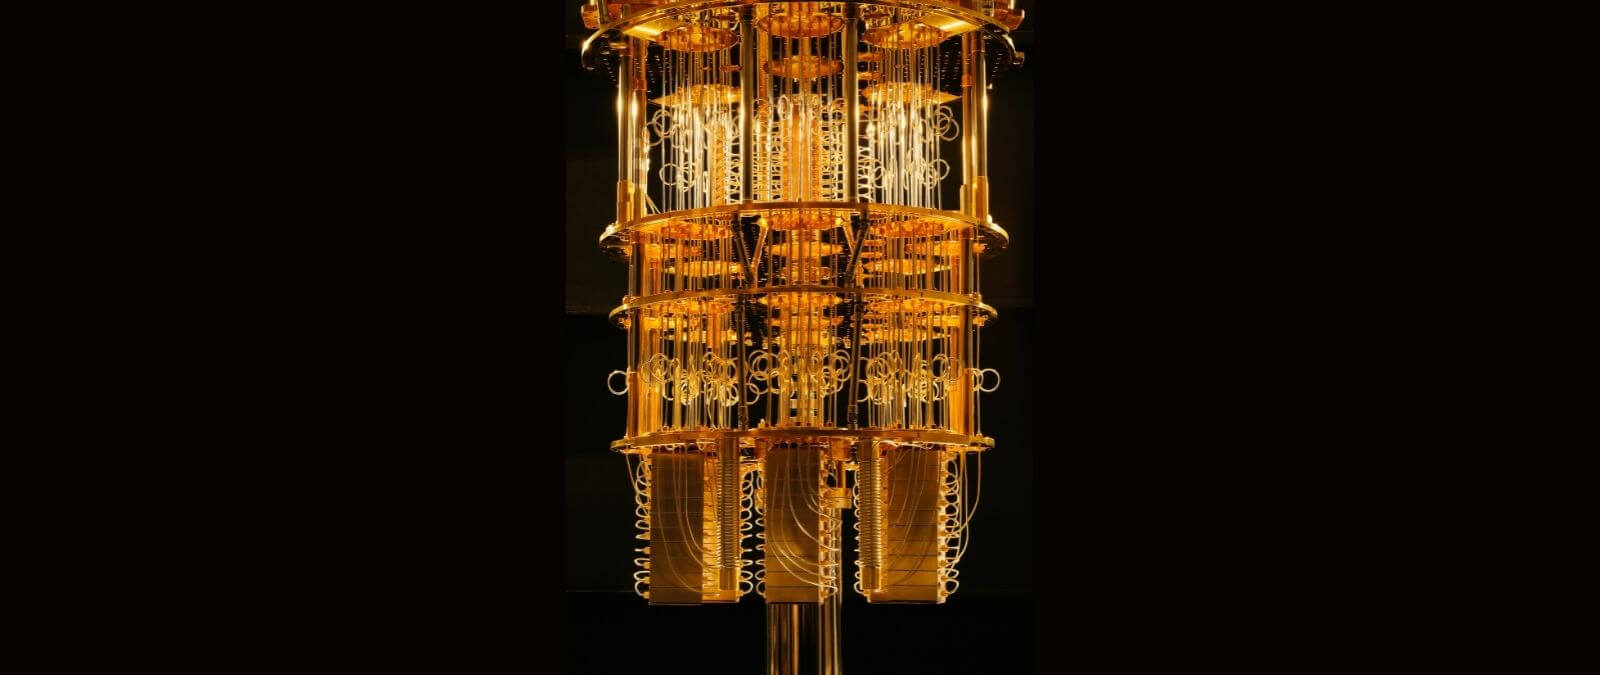
\includegraphics[width=1\linewidth]{Figuras/Fig_ordenador_cuantico.png}
	%\end{figure}


	\begin{figure}[b]
	\centering 
	
\includegraphics[width=1\linewidth]{Figuras/Fig-Logo_QS_EspanaDigital.png}
	
\includegraphics[width=1\linewidth]{Figuras/Fig-LOGOS-GOB_QS.png}
	\end{figure}

\newpage
\thispagestyle{empty}
\mbox{}

\newpage
\pagestyle{plain}
\tableofcontents
\newpage



% TABLA DE ABREVIATURAS





% \chapter{Introduccion matemática}
% Bases, multiplicación de matrices, autovectores,...

% \chapter{Información cuántica}
% seguir las lecciones de qiskit https://www.youtube.com/playlist?list=PLOFEBzvs-VvqKKMXX4vbi4EB1uaErFMSO
%	\section{Sistemas simples}
% 		\section{Información clásica}
% 		Introducir la notación de dirac comparando con los vectores $\hat{x}, ...
%
%	\subsection{Sistemas múltiples}



\addcontentsline{toc}{chapter}{Introducción}
\chapter*{Introducción}

En estas notas vamos a ver una introducción a la Computación Cuántica y los algoritmos cuánticos más famosos. En las mismas, se presentará todo lo necesario para entender estos algoritmos suponiendo que el lector no tiene conocimiento alguno sobre Mecánica Cuántica ni Computación Cuántica. 

La parte \ref{part_conceptos_basicos} de estas notas se dedica a introducir los Conceptos Básicos necesarios para entender el resto de las mismas. Esto incluye una introducción al formalismo matemático (capítulo \ref{cap_formalismo}), donde se verán los conceptos matemáticos necesarios para abordar el segundo capítulo de esta parte, una introducción a la Mecánica Cuántica (capitulo \ref{cap_fundamentos}). 


Después de estos dos capítulos introductorios, pasamos a la parte \ref{part_fundamentos_cc}, donde damos una introducción a las Fundamentos de la Computación Cuántica: qúbits, puertas, medidas, circuitos, hardware, decoherencia, $\dots$.


Finalmente, cerramos las notas con la parte \ref{part_algoritmos}, donde presentando de forma detallada los algoritmos más famosos. Esto incluye el algoritmo de Quantum Fourier Transform (capítulo \ref{chapter_QFT}), el de Estimación Cuántica de Fase (capítulo \ref{chapter_QPE}) y los archiconocidos algoritmos de Grover (capítulo \ref{chapter_Grover}) y Shor (capitulo \ref{chapter_Shor}). Además hablaremos también de Criptografía y Quantum Key Distribution (capítulo \ref{chapter_QKD}). 

Como veremos a lo largo de estas notas, los algoritmo en computación cuántica se basan en construir \textbf{circuitos cuánticos} a los que añadimos \textbf{puertas cuánticas}. A estos circuito se les pasa como entrada un \textbf{estado cuántico}. Las puertas de circuito operan sobre el estado y nos devuelven otro estado cuántico. Este último representará la solución de nuestro problema, mientras que el circuito representa el \textbf{algoritmo cuántico} que se usa para hallar la solución. La idea es bastante similar a la de la computación clásica, donde se parte de una cadena bit, se aplican una serie de puertas lógicas (AND, OR, NOT,...) y se obtiene otra cadena de bits que codifica la solución. 

Como veremos más adelante, la computación cuántica (al igual que la clásica) es un paradigma de \textbf{computación universal}. Es decir, al menos sobre el papel, todo lo que se puede calcular con un ordenador clásico (todo lo que es \textbf{computable}), se puede calcular con un ordenador cuántico. La gran diferencia entre estos dos modelos es que el primero aprovecha las propiedades exóticas de la mecánica cuántica (superposición y entrelazamiento) para plantear algoritmo más rápidos que los clásicos. De esta forma, la computación cuántica tiene el potencial de acelerar ciertos cálculos. 


	\begin{mybox_blue}{Nota: Paradigmas de Computación Cuántica}
	Habitualmente cuando se habla de \textbf{computación cuántica} se suele hablar de la \textbf{Computación 
	Cuántica basada en Puertas}. Los otros dos paradigmas de computación cuántica son la \textbf{Computación
	Cuántica Adiabática} y el \textbf{Quantum Anneling}. Los dos primeros son paradigmas de computación
	universal mientras que el Quantum Anneling no lo es. \vspace{0.3cm}
	
	En estas notas hablaremos solo de Computación Cuántica basada en Puertas, a partir de ahora simplemente
	computación cuántica o QC (del inglés, Quantum Computing).
	\end{mybox_blue}	




\newpage

\addcontentsline{toc}{section}{Código de colores}
\section*{Código de colores} %%Omitir_seccion

\begin{mybox_gray2}{}
Teoremas, Lemmas, Definiciones, Demostraciones y conceptos importantes
\end{mybox_gray2}

\begin{mybox_gray}{Cuadros grises con bordes}
Ejercicios
\end{mybox_gray}

\begin{mybox_blue}{Cuadros azules}
Notas o aclaraciones
\end{mybox_blue}

\begin{mybox_green}{Cuadros verdes}
Ejemplos
\end{mybox_green}

\begin{mybox_orange}{Cuadros naranjas}
Referencias a cuadernos de Jupyter Notebook
\end{mybox_orange}


\part{Conceptos básicos}	 \label{part_conceptos_basicos}

\chapter{Formalismo matemático} \label{cap_formalismo}

La Mecánica Cuántica (así como la Computación Cuántica) hace uso de unas matemáticas con las que es necesario familiarizarse. En esta capítulo vamos a repasar el formalismo matemático básico para el resto del curso.
 
A pesar de que la expresión ``formalismo matemático'' puede llegar a imponer respeto, a lo largo de este capítulo veremos que las cosas son más simples de lo que pudieran parecer en un principio. La Mecánica Cuántica  alcanza unos niveles de complejidad matemática insospechados, pero al mismo tiempo es sorprendente como se pueden entender los fundamentos de la misma con una serie de pinceladas de ciertos conceptos matemáticos: \textit{numeros complejos}, \textit{vectores}, \textit{operadores (matrices)}, \textit{tensores} y algo de \textit{probabilidad}.

Los conceptos que se presentan a continuación están un pasito por encima del nivel de matemáticas de bachillerato, pero no mucho más. Nuestro objetivo es entender las bases de la Mecánica Cuántica, sin llegar a plantearnos trabajar de forma seria con sus ecuaciones. Es decir, ser capaces de entender los conceptos y trabajar con las soluciones, no con las ecuaciones. Por este motivo, los conceptos matemáticos más complejos como integrales o resolución de ecuaciones diferenciales están más allá del objetivo de este curso.

En resumen, no hay que tener miedo a las matemáticas de este curso, son sencillas. 

Este capítulo se basa en \cite{Curso-JMas}, que a su vez toma como referencias los capítulo 2 de  \cite{Claude}, \cite{le_bellac_2006} y \cite{khatri2020principles}

	\section{Números complejos}
		
		\subsection{Introducción}
		
Para entender de donde surge la idea de los número complejos, tenemos que recordar primero que el cuadrado de cualquier número real, $a \in \mathbb{R}$, es \textit{siempre} positivo: $a^2 > 0$. Por ejemplo
	\begin{equation*}
	2^2 = (-2)^2 = +4
	\end{equation*}
Por eso, la raíz cuadrada de un número real \textit{sólo} existe (como número real) si el número es positivo y tiene dos soluciones, la positiva y la negativa:
	\begin{equation*}
	\sqrt{4} = \pm 2
	\end{equation*}
En este punto, surge la siguiente pregunta: cual es la solución de la siguiente ecuación?
	\begin{equation}
	x^2 + 1 = 0 \rqa x^2 = -1 \rqa x = \sqrt{-1}
	\end{equation}
Como comentamos, no hay ningún número real que cumpla esa ecuación. Podemos pues, definir un nuevo número. Este número no pertenece a los números reales:

	\Definicion{Se postula la existencia de un número, $i$, que es solución de la ecuación
		\begin{equation}
		i^2 = -1
		\end{equation}}

Equivalentemente $i = \sqrt{-1}$. No hay nada misterioso en $i$, se puede sumar, restar, multiplicar y dividir normalmente:
	\begin{align*}
	i + i & = 2i \\
	i - i & = 0 \\
	i + 2i & = 3i \\
	i^3 & = i^2 \cdot i = -i \\
	i^4 & = i^2 \cdot i^2  = 1 \\
	\frac{i}{i} & = 1
	\end{align*}

Una vez definido este número, podemos resolver cualquier raíz con un número negativo:
	\begin{equation}
	x^2 + 4 = 0  \rqa x = \sqrt{-4} = \sqrt{4} \sqrt{-1} = 2i
	\end{equation}

En resumen: la solución pasa por ampliar el conjunto de los número reales definiendo un nuevo conjunto, el de los \textbf{números imaginarios} o \textbf{complejos}, $\mathbb{C}$


		\subsection{Forma cartesiana, polar y conjugación compleja}

Los números complejos pueden escribirse de dos formas diferentes: la forma \textbf{cartesiana} y la forma \textbf{polar}.

	
			\SubsubiIt{Forma cartesiana}

\begin{mybox_gray2}{}
Un \textit{número complejo}, $z \in \mathbb{C}$, se representa en la \textbf{forma cartesiana} mediante dos números reales $x,y \in \mathbb{R}$,
	\begin{equation}
	z = x + iy \hspace{0.5cm} \text{donde} \hspace{0.5cm} 
	\lch 
	\begin{split}
	x & \quad \text{ es la \textit{parte real}} \\
	y & \quad \text{ es la \textit{parte imaginaria}} \\
	\end{split}
	\right.
	\end{equation}
\end{mybox_gray2}



Como podemos ver, tenemos dos casos:
\begin{itemize}
	\item Si $y=0 \rightarrow z = x$ es un \textbf{número real puro}. 
	\item Si $x = 0 \rightarrow z = iy$ es un \textbf{número imaginario puro}.
\end{itemize}
Aquí podemos ver perfectamente que los número complejos (o imaginarios) son una extensión de los números reales, en el sentido de que los engloban: como acabamos de ver, un número real puede verse como un número complejo con la parte imaginaria igual a cero.


Es bien conocido que los números reales se representan sobre una recta, la \textbf{recta real}. Los números complejos por su parte se representan en un plano, el \textbf{plano complejo}, donde el eje horizontal es la recta real y el eje vertical es el eje imaginario. Esto se ve precisamente muy bien en la forma cartesiana, pues $x$ sería el valor del eje real e $y$ sería el valor del eje imaginario. Podemos ver esto más claramente en la Fig. \ref{Fig_formalismo_Complex_number_illustration_modarg}. 

\begin{figure}[H] \setcounter{subfigure}{0}
\centering
\subfigure[Representación de un número $z=a+bi$ en el plano complejo. \label{Fig_formalismo_Complex_number_illustration}]{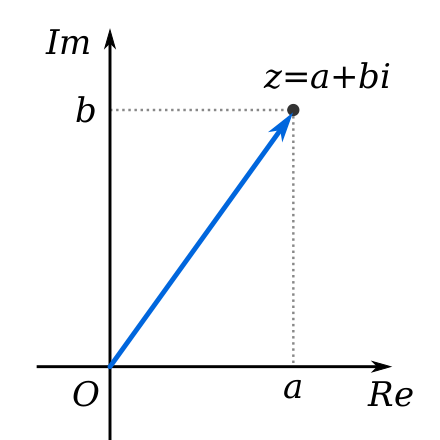
\includegraphics[width=0.3\linewidth]{Figuras/Fig_formalismo_Complex_number_illustration.png}}
\hspace{0.5cm}
\subfigure[Representación polar de un número complejo $z = x +iy$. En el texto se usan $\rho$ y $\theta$ en lugar de $r$ y $\phi$, pero es lo mismo. \label{Fig_formalismo_Complex_number_illustration_modarg}]{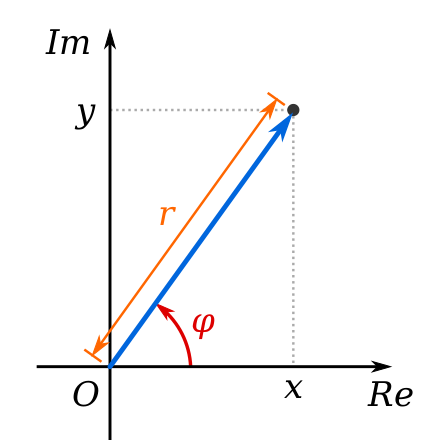
\includegraphics[width=0.3\linewidth]{Figuras/Fig_formalismo_Complex_number_illustration_modarg.png}}
\hspace{0.5cm}
\subfigure[Un número complejo y su conjugado \label{Fig_formalismo_conjugación}]{\includegraphics[width=0.3\linewidth]{Figuras/Fig_formalismo_conjugación.png}}
\caption{Representaciones de números en el plano complejo.}
\end{figure}
		
			
			\SubsubiIt{Forma Polar}
			
	\Teorema{Dado un ángulo $\theta \in [0,2 \pi)$ las dos expresiones siguientes son equivalentes
	\begin{equation}
	\cos \theta + i \sin \theta = e^{i \theta}
	\end{equation}
	A esta identidad se la denomina \textbf{Fórmula de Euler}.}
	
	\begin{proof}
	La demostración de la Fórmula de Euler viene de expandir ambos miembros en serie de Taylor en torno a $\theta = 0$ y comprobar que ambas series son iguales
	$$
	\begin{array}{rcl}
	e^{i\theta} &=& 1 + i\theta + \frac{1}{2}(i\theta)^2 + \frac{1}{3!}(i\theta)^3+\, ... \\
    &=& 1 -\frac{1}{2}\theta^2 ~+~ ... ~+~ i \left(\theta - \frac{1}{3!} \theta^3+ \, ...\right) \\
    &=& \cos \theta  + i \sin \theta 
	\end{array} 
	$$
	\end{proof}

Con esto, veamos lo que es la forma polar:
	\begin{mybox_gray2}{}
	El número $z=x + i y$ se puede representar en \textbf{forma polar}
		\begin{equation}  \label{ec_formalismo_forma_polar}
		z = \rho e^{i\theta} = \rho (\cos\theta + i \sin\theta)  
		\end{equation}
	de donde obtenemos las componentes cartesianas 
		\begin{equation}
		x=\rho\cos\theta ~~,~~y=\rho\sin\theta.
		\end{equation}
 	Tanto $\rho$ como $\theta$ son números reales y se denominan \textbf{módulo} y \textbf{fase}.
	\end{mybox_gray2}
	
	En principio, esta forma de representar los números complejos puede parecer rara, pero es muy fácil de entender. Para ello, solo hay que recordar que los números complejos los podemos representar en un plano. Los puntos en un plano pueden verse como \textbf{vectores} que parten del origen y cuya punta acaba en el punto que queremos describir. La forma habitual de referirse a estos vectores (puntos) es usar las coordenadas sobre los dos ejes, es decir, usar lo que en matemáticas se llama \textbf{sistema de coordenadas cartesiano} (ver la Fig. \ref{Fig_formalismo_Complex_number_illustration_modarg}). Sin embargo, otra forma de describir estos puntos es usando el módulo del vector (su longitud) y el ángulo que este forma con el eje horizontal (ver la Fig. \ref{Fig_formalismo_Complex_number_illustration_modarg}). A esta forma de describir el plano se la llama \textbf{sistema de coordenadas polar}.
	
	La forma polar que acabamos de ver de los número complejos (Ec. \ref{ec_formalismo_forma_polar}) no es más que describir el número complejo usando el sistema de coordenadas polar. En concreto, el número real $\rho$ es el módulo del vector y el número real $\theta$ es su fase, es decir, el ángulo con el eje horizontal. Usando el \textbf{teorema de Pitágoras} para los triángulos rectángulos es muy fácil comprobar que $\rho$ es el módulo si tenemos en cuenta que $x$ e $y$ son los catetos:
	$$
	x^2 + y^2 = \rho^2 \cos^2 \theta + \rho^2 \sin^2 \theta = \rho^2 (\cos^2 \theta +  \sin^2 \theta) =  \rho^2.
	$$

	\begin{mybox_blue}{Números con módulo 1}
	Como ya comentamos, a $\theta$ se le denomina \textbf{fase}. Habitualmente también se denominan fases a los números complejos con $\rho =1$ pues en estos casos tenemos $z = e^{i \theta}$. Esto es un abuso del lenguaje pero es algo muy extendido.
	\end{mybox_blue}

		
			\SubsubiIt{Conversión entre forma cartesiana y polar}

La conversión de la representación \textit{polar a cartesiana} es muy sencilla gracias a las fórmula de Euler
	\begin{equation}
	\boxed{z = r e^{i\theta} = x + i y ~~~\hbox{ con }  ~~~\left\{\begin{array}{l} x=r \cos \theta \\ \rule{0mm}{4mm} y = r\sin \theta . \end{array} \right. }
	\end{equation}
La conversión inversa, \textit{de cartesiana a polar} es un poco más delicada. Formalmente sería
	\begin{equation} \label{ec_formalismo_de_cartesiana_a_polar}
	\boxed{z = x + i y  = r e^{i\theta} ~~~ \hbox{ con } ~~~ \left\{\begin{array}{l} r=\sqrt{x^2+y^2} \\  \rule{0mm}{4mm} \theta = \arctan(y/x) . \end{array} \right.} 
	\end{equation}

	\begin{mybox_blue}{Signo de la arcotangente}
	En la formula de la arcotangente de la Ec. (\ref{ec_formalismo_de_cartesiana_a_polar}) hay que elegir el signo con cuidado. La arcotangente devuelve valores en $(-\pi/2$, $\pi/2)$, pero sabemos que los ángulos en la circunferencia está en  $[0,2\pi)$. Por ello, hay que aplicar el siguiente criterio:
	\begin{itemize}
		\item Si $x=0$ e $y>0$ (sobre el eje $y$) $\Rightarrow \theta = \pi$
		\item Si $x=0$ e $y<0$ (sobre el eje $y$) $ \Rightarrow \theta = 3\pi/2$
		\item Si $x>0$ e $y \geq 0$ (primer cuadrante) $ \Rightarrow \theta = \arctan (y/x)$
		\item Si $x<0$ e $y \geq 0$ (segundo cuadrante) $ \Rightarrow \theta = \arctan (-y/x) + \pi/2$
		\item Si $x<0$ e $y<0$ (tercer cuadrante) $ \Rightarrow \theta = \arctan (y/x) + \pi$
		\item Si $x<0$ e $y<0$ (cuarto cuadrante) $ \Rightarrow \theta = \arctan (-y/x) + 3\pi/2$
	\end{itemize}
	\end{mybox_blue}

	\Ejercicio{Calcula a mano la forma polar de los números: 
	$$
	4 + 3i, \quad 7 - 2i, \quad - 5 + 5i, \quad - 3 + 4i
	$$}
			
			
			\SubsubiIt{Conjugación compleja}

Todo número complejo, $z$, lleva \textit{asociado} otro, $z^*$, denominado el \textbf{complejo conjugado} que se obtiene cambiando $i \to -i$, tanto en forma cartesiana
	\begin{equation}
	\boxed{z = x+i y ~~~~\leftrightarrow~~~~ z^* = x - i y}
	\end{equation}
como en forma polar
	\begin{equation}
	\boxed{z = \rho e^{i \theta} ~~~~\leftrightarrow~~~~ z^* = \rho e^{- i \theta}}
	\end{equation}

Hablando de representaciones, la conjugación compleja no es más que una reflexión sobre el eje horizontal como podemos ver en la Fig. \ref{Fig_formalismo_conjugación}.

Matemáticamente, el complejo conjugado $z^*$ de un número complejo $z$ es el número por el cual hay que multiplicar $z$ para obtener el módulo cuadrado, es decir:
	\begin{equation}
	\boxed{|z|^2 = z \cdot z^* = \rho^2}
	\end{equation}
			
			
		\subsection{Operaciones básicas}

Los números complejos ${\mathbb C}$ forman una estructura matemática denominada \textit{cuerpo}. Esto  quiere decir que admiten dos operaciones \textit{internas}: la \textbf{suma} y la \textbf{multiplicación}. Vamos a estudiarlas por separado


			\SubsubiIt{Suma}

\begin{itemize}
	\item En \textit{forma cartesiana} se \textit{suman las partes real e imaginaria por separado}
	\begin{equation}
(a + i b) + (c + i d) = (a+c) + i (b+d)
	\end{equation} 
La resta es obvia, ya que $a,b,c,d$ pueden ser números negativos. 	

	\item En  \textit{forma polar}, la suma de dos números complejos no admite ninguna simplificación, y deben transformarse primeramente a forma cartesiana, para sumarse. 
	\begin{equation}
z + w = \rho e^{i\theta} + \sigma e^{i\phi} = (\rho\cos\theta + \sigma\cos\phi) + i(\rho\sin\theta +  \sigma\sin\phi) 
	\end{equation}	
\end{itemize}
			
			\SubsubiIt{Multiplicación}

\begin{itemize}
	\item En \textit{forma cartesiana} debemos multiplicar todos los factores entre sí, y teniendo en cuenta que $i^2= -1$
	\begin{equation}
(a + i b) (c + i d) =ac +  ai d +i bc +i^2 bd = (ab - bd) + i(ac + bd)
	\end{equation} 

	\item En la \textit{forma polar}, la cosa es más simple, pues solo hay que multiplicar los módulos y sumar las fases: 
	\begin{equation}
z w = r e^{i\theta} s e^{i\phi} = rs\,   e^{i(\theta + \phi)} 
	\end{equation}
\end{itemize}

			\SubsubiIt{Valor absoluto}

El cuadrado de un número real $a\in {\mathbb R}$ es otro número real positivo $a^2 >0$. Ello nos permite definir
el valor absoluto $|a| = \sqrt{a^2}$ que es el mismo para $a$ y para $-a$.

Esto no sucede con un número complejo $z$. En efecto,  $z^2 = x^2 - y^2 +2i xy$ es complejo. Sin embargo, el producto de un número por su conjugado es un número \textit{real} y \textit{positivo}
$$
z z^*  = (x + i y) (x-i y) = x^2 + y^2 >0
$$
lo nos permite definir el \textbf{valor absoluto} de un número complejo
	\begin{equation}
	\boxed{|z| = \sqrt{z z^*} = \sqrt{x^2 + y^2}}
	\end{equation}

El valor absoluto de una fase es 1
	\begin{equation}
	|e^{i\theta}| = \sqrt{ e^{i\theta}   e^{-i\theta}}=\sqrt{ e^{i(\theta-\theta)}}=\sqrt{e^0} = 1
	\end{equation}
El valor absoluto de un número complejo coincide con el \textbf{módulo} escrito en forma polar
	\begin{equation}
	|z| = \sqrt{zz^*} = \sqrt{\rho e^{i\theta} \rho e^{-i\theta}}=\sqrt{\rho^2} ~~ \Rightarrow ~~ \boxed{|z| = \rho}
	\end{equation}

			
			\SubsubiIt{División}
			
Al igual que la multiplicación, en forma cartesiana, la división no es simple. Sea $z = a+ i b$ y $w=c+i d$ 
	\begin{equation}
	\frac{z}{w} = \frac{z}{w}\frac{w^*}{w^*} = \frac{( a+ i b)(c-i d)}{|w|^2} = \frac{ac+bd + i(bc-ad)}{c^2+d^2}  = \frac{ac+bd}{c^2+d^2} +i\frac{bc-ad}{c^2+d^2}
	\end{equation}

En forma polar la división es tan sencilla como la multiplicación. Se toma el  cociente de los módulos y la resta de las fases
	\begin{equation}
	\frac{z}{w} = \frac{\rho e^{i\theta}}{\sigma e^{i\phi}} = \frac{\rho}{\sigma} e^{i(\theta-\phi)}
	\end{equation}


			
		\subsection{Casos particulares}
		
			\SubsubiIt{Sumas nulas}
			
En muchas ocasiones nos encontraremos la siguiente representación del numero cero (complejo) $0 = 0 + i 0$
	\begin{equation}
\sum_{k=0}^{N-1} e^{2\pi i k/N} =   e^{2\pi i\, 0/N} +  e^{2\pi i\, 1/N}  +~...~ +   e^{2\pi i\, (N-2)/N}+   e^{2\pi i\, (N-1)/N} ~=~  ~0.
	\end{equation}
No es trivial ver que esta igualdad es cierta, así que no vamos a demostrarla.
			
Si multiplicamos todas la fases por un número entero $j$ tal que $1\leq j \leq N-1$, el resultado es el mismo
$$
\sum_{k=0}^{N-1} e^{2\pi i j k/N} =   e^{2\pi i \, 0/N} +  e^{2\pi i \, j/N}  +~...~ +   e^{2\pi i \, j(N-2)/N}+   e^{2\pi i \, j(N-1)/N} ~=~  ~0.
$$

Sin embargo si $j = 0, N, 2N,... = 0\,\hbox{mod} N$, entonces \textbf{la suma no se anula} y su valor es igual a $N$. Tomemos por ejemplo $j=N$ 
$$
\sum_{k=0}^{N-1} e^{2\pi i (N) k/N} = \sum_{k=0}^{N-1} e^{2\pi i  k}  =  \sum_{k=0}^{N-1} 1 =~  ~N.
$$

Una manera de resumir todos los casos anteriores en una sola expresión involucra la función $\delta$ \textbf{de Kronecker}
	\begin{equation} \label{ec_fundamentos_delta_de_kronecker}
	\delta_{ij} = \left\{ \begin{array}{rcl} 0 & \hbox{si} & i\neq j \\ 1 & \hbox{si} & i = j \end{array} \right.
	\end{equation}
Con ella podemos enunciar el siguiente resultado 
	\begin{equation}
	\boxed{\frac{1}{N}\sum_{k=0}^{N-1} e^{2\pi i \, j k/N} =  \delta_{j\, 0{\rm mod} N}},
	\end{equation}
que usaremos al estudiar la transformada de Fourier cuántica.
			
			\SubsubiIt{Desigualdad triangular}
			
\begin{mybox_gray2}{}			
\textbf{Desigualdad triangular}:

El módulo de la suma de dos números complejos verifica que
$$
| z+w| \leq |z| + |w| \,
$$
donde la igualdad sólo se verifica cuando ambos números complejos son paralelos en el plano complejo. 
\end{mybox_gray2}
	
	
	
	\section{Vectores}
		
		\subsection{Espacio Vectorial Complejo}
		
			\SubsubiIt{Definición}
			
	\Definicion{
	De forma poco rigurosa, definiremos un \textbf{vector de dimensión} $N$ como una columna de $N$ números complejos 
$$
|u\rangle = \begin{bmatrix} {u_1}\\ {u_2}\\ \vdots \\ {u_N} 
\end{bmatrix}
$$
	}
\begin{itemize}
	\item El símbolo $\ket{u}$  \textit{representa }al vector y se denomina \textbf{ket} en la \textbf{notación de Dirac}. Otra notación sería $\vec{u}$, pero esta nunca se usa en Mecánica Cuántica.

	\item Los números complejos $u_i \in {\mathbb C}$ con $\, i=1,...,N$ se denominan \textbf{componentes} del vector $\ket{u}$. Estas componentes toman un valor concreto cuando especificamos una \textbf{base}. En otra base, estos elementos pueden tener otro valores. Es decir, el vector es un objeto abstracto.
\end{itemize}
			
	\Definicion{
	La colección de todos los posibles vectores de $N$ componentes,  con las  propiedades de suma y multiplicación forman un \textbf{espacio vectorial}, $V$ de dimension compleja $N$.
	}			

Es decir,  en un espacio vectorial  tenemos las siguientes propiedades:
	\begin{itemize}
	\item Dos operaciones posibles: \textbf{suma }de dos vectores y \textbf{multiplicación de un vector por un número complejo }$\lambda\in {\mathbb C}$
	\begin{equation}
 |u\rangle + \ket{v}~ =~\, 
\begin{bmatrix} {u_1}+v_1\\ {u_2}+v_2\\ \vdots \\ {u_N}+v_n \end{bmatrix} ~= ~\ket{w}\ , \qquad \lambda|u\rangle ~ =~   \begin{bmatrix} {\lambda u_1}\\ {\lambda u_2}\\ \vdots \\ {\lambda u_N} \end{bmatrix} ~\equiv~\ket{\lambda u}
	\end{equation}
	
	\item Existencia de un \textbf{elementos neutro} (respecto a la suma). Todo vector de $V$ se denota mediante el símbolo $\ket{v}$ menos el elemento neutro, que se escribe como $0$.
		\begin{equation}
			\ket{v} + 0 = \ket{v}
		\end{equation}
	
	\item La existencia de un \textbf{elemento opuesto} (respecto a la suma):
		\begin{equation}
		\ket{v} + \ket{-v} = \ket{v}-\ket{v} = 0
		\end{equation}
	\end{itemize}

	\begin{mybox_blue}{Dimensión de un espacio vectorial complejo}
	La \textbf{dimensión} es igual al número de cantidades (\textit{grados de libertad}) que debemos fijar para especificar un vector. Como estamos lidiando con un espacio vectorial complejo donde nuestro vector está compuesto por $N$ números complejos, la cantidad de números reales que debemos fijar es $2N$.
   \vspace{0.3cm}
   
Entonces, podemos decir que la \textbf{dimensión compleja} de un espacio vectorial complejo $V$ es $N$, o que su \textbf{dimensión real} es $2N$ 
	\begin{equation}
	{\rm dim}_{\mathbb C} V = N ~~~~\Longleftrightarrow ~~~   {\rm dim}_{\mathbb R} V = 2N
	\end{equation}
Habitualmente, cuando se habla simplemente de \textit{dimensión} se habla de la real.
	\end{mybox_blue}	
	
		\SubsubiIt{Conjugación adjunta}
		
La operación \textbf{conjugación adjunta},  $\dagger$, es una \textit{extensión} de la \textbf{conjugación compleja}  a los vectores.

	\Definicion{Asociado a cada \textit{ket }$\ket{u}$, definimos un vector \textbf{adjunto}, o \textbf{bra} $\bra{u}\equiv\left(\ket{u}\right)^\dagger$,  que representamos mediante un vector fila con las componentes conjugadas complejas:  
		\begin{equation}
\dagger \,: \quad\,|u\rangle = \begin{bmatrix} {u_1}\\ {u_2}\\ \vdots \\ {u_N} \end{bmatrix} 
~~~~~{\rightarrow}~~~~~~ \left(\ket{u}\right)^\dagger \equiv \bra{u} =\begin{bmatrix} {u_1^*} & {u_2^*} & \cdots & {u_N^*}
\end{bmatrix}
		\end{equation}
	}

Consistentemente encontramos para el producto de un vector por un número complejo $\lambda$
	\begin{equation}
	\dagger \,:\quad\,  \lambda\ket{u}=\ket{\lambda u} ~~~~~{\rightarrow}~~~~~~ \left(\lambda\ket{u}\right)^\dagger=\lambda^*\bra{u} = \bra{u}\lambda^* = \bra{\lambda u}
	\end{equation}
ya que el producto de un vector por un número es conmutativo.		
		
	\begin{mybox_blue}{Notación}
	En la notación con \textit{kets} y \textit{bras} vemos que es lo mimos escribir $\lambda\ket{u}$ que $\ket{\lambda u}$. Esto podemos pensarlo como que los números complejos entran y salen de los kets sin modificaciones. 
	\vspace{0.3cm}
	
	Sin embargo, en los bras tenemos $\bra{u}\lambda^* = \bra{\lambda u}$. Es decir, sacar o meter un número complejo dentro de los bras implica una conjugación compleja del número. 
	\vspace{0.3cm}
	
	Esto, como comentamos, es solo \textbf{notación}, es decir, un convenio para escribir las cosas.
	\end{mybox_blue}
		
Al igual que la conjugación compleja, la conjugación adjunta es una \textbf{involución}: su aplicación sucesiva devuelve el vector original
$$
(\ket{u}^\dagger)^\dagger =\bra{u}^\dagger =  \ket{u}
$$
es decir, $\dagger^2 = I$, el operador identidad.		
		
		
		\subsection{Bases}
		
	\Definicion{
	En un espacio vectorial $V$ de dimensión $N$ una \textbf{base} es una colección de $N$ vectores  $\{\ket{e_1},...,\ket{e_N}\}$ tales que, cualquier vector $\ket{v}\in V$ se puede expresar como una \textbf{combinación lineal} de ellos
$$
\ket{v} = \sum_{i=1}^N v_i \ket{e_i}
$$  
Los coeficientes $v_i$ son las \textbf{componentes} de $\ket{v}$ \textit{en la base dada}.
	}		
	
Existen \textit{infinitas bases} en un espacio vectorial. Podemos escoger una de ellas y asociarle el siguiente conjunto de columnas
	\begin{equation} \label{ec_formalismo_base_cartesina}
|e_1\rangle \sim \begin{bmatrix} 1 \\ 0 \\ 0\\ \vdots 
\\ 0 \\ 0 \end{bmatrix}~~~~
|e_2\rangle \sim \begin{bmatrix} 0 \\ 1 \\ 0\\ \vdots 
\\ 0 \\ 0 \end{bmatrix}~~~~~~~~~
\cdots ~~~~~~~~
|e_{N-1}\rangle \sim \begin{bmatrix} 0 \\ 0 \\ 0\\\vdots 
\\ 1 \\ 0 \end{bmatrix}~~~~
|e_N\rangle \sim \begin{bmatrix} 0 \\ 0 \\0\\ \vdots 
\\ 0 \\ 1 \end{bmatrix}
	\end{equation}


De esta forma, cualquier vector, escrito como una combinación lineal de sus elementos adquiere la representación usual
	\begin{align}
	|u\rangle ~&=~ {u_1} |e_1 \rangle + {u_2} | e_2\rangle +... + {u_{ N}}|e_{ N}\rangle~=~ \sum_{i=1}^N {u_ i} |e_i\rangle \,\sim \\
	\sim &~ {u_1} \begin{bmatrix} 1 \\ 0 \\ 0\\ \vdots 
\\ 0 \\ 0 \end{bmatrix} \,+\,{u_2} \begin{bmatrix} 0 \\ 1 \\ 0\\ \vdots \\ 0 \\ 0 \end{bmatrix}~+~ ... ~+ ~
{u_{N-1}} \begin{bmatrix} 0 \\ 0 \\ 0\\\vdots 
\\ 1 \\ 0 \end{bmatrix}+ 
\,{u_N}\,  \begin{bmatrix} 0 \\ 0 \\0\\ \vdots 
\\ 0 \\ 1 \end{bmatrix}~~~= ~~~
  \begin{bmatrix} {u_1} \\ {u_2} \\{u_3}\\ \vdots 
\\ \,{u_{N-1}}\, \\ {u_{N}} \end{bmatrix}
	\end{align}

		
			\SubsubiIt{Cambio de base}

Existen \textit{infinitas} bases  en un espacio vectorial de dimensión finita.
Todas ellas sirven para representar un vector arbitrario.

Consideremos dos bases 
$\{\ket{e_i}\}$ y $\{\ket{f_j}\}$ donde $ i,j = 1,...,N$.
Cualquier vector $\ket{v}$ se puede expandir de forma diferente en cada una de ellas
$$
\ket{v} ~=~ \sum_{i=1}^N v_i \ket{e_i} ~=~ \sum_{i=1}^N \tilde v_i \ket{f_i}
$$
donde las componente $v_i$ y $\tilde v_i$ \textit{deben ser distintas} pero \textit{estar relacionadas}. Es decir, las componentes de los vectores dependen de la base elegida y tiene una \textit{regla de cambio} cuando decidimos escribir nuestro vector en otra base.
		
Para encontrar esta relación entre los elementos del vector en distintas bases tenemos que primero encontrar la relación entre la  bases. Como ya dijimos, cualquier vector se puede escribir como combinación lineal de elementos de una base, sin ninguna excepción. Es decir, como caso particular tenemos que cualquier elemento (vector) de una base se puede expresar como una combinación lineal de elementos de la otra. Tomemos por ejemplo, $\ket{v}= \ket{f_1}$
	\begin{equation}
	\ket{f_1} = \sum_{i=1}^N A_{ i 1} \ket{e_i}
	\end{equation}
donde $A_{ i 1}\in \mathbb{C}$ son las componentes del vector $\ket{f_1}$ en la base $\{\ket{e_i}\}$. Haciendo esto para todos los elementos de la base $\{\ket{f_j}\}$, los coeficientes constituyen una \textbf{matriz de cambio de base} $A_{ij}$:
	\begin{equation} \label{ec_formalismo_cambio_base_base}
	\boxed{\ket{f_j} = \sum_{i=1}^N A_{ i j} \ket{e_i} ~,~~~~~~j=1,..., N}
	\end{equation}
	\begin{mybox_blue}{Nota}
	La forma en que están sumados los índices $\ket{f_j} = \sum_{i=1}^N A_{ \textcolor{red}{i} j} \ket{e_{\textcolor{red}{i}}}$.
	\end{mybox_blue}
Dado un vector $\ket{v}$ con coordenadas $(v_1,\dots,v_N)$ en la base $\{\ket{e_i}\}$ y coordenadas $(\tilde{v}_1,\dots,\tilde{v}_N)$ en la base $\{\ket{f_i}\}$, es decir,
$$
\ket{v} ~=~ \sum_{i=1}^N v_i \ket{e_i} ~=~ \sum_{i=1}^N \tilde{v}_i \ket{f_i}
$$
la fórmula de cambio de base expresa las coordenadas sobre la base antigua, $\{\ket{e_i}\}$, en términos de las coordenadas sobre la base nueva, $\{\ket{f_i}\}$:
	\begin{equation} \label{ec_formalismo_cambio_de_base}
	\boxed{v_i = \sum_{i=1}^N A_{ij} \tilde{v}_j}
	\end{equation}
	\begin{mybox_blue}{Nota}
	La forma en que están sumados los índices $v_i = \sum_{i=1}^N A_{i\textcolor{red}{j}} \tilde{v}_{\textcolor{red}{j}} $.
	\end{mybox_blue}
En términos de matrices, la formula de cambio de base es
	\begin{equation}
	\boxed{\ket{v}_{\{\ket{e_i}\}} = A \ket{v}_{\{\ket{f_i}\}}}
	\end{equation}
	donde $\ket{v}_{\{\ket{e_i}\}}$ y $\ket{v}_{\{\ket{e_i}\}}$ son los vectores columna con las coordenadas de $\ket{v}$  en las bases $\{\ket{e_i}\}$ y $\{\ket{f_i}\}$ respectivamente. 
	\begin{proof}
	Usando definición (\ref{ec_formalismo_cambio_base_base}) de la matriz de cambio de base, tenemos
	\begin{align*}
	\ket{v} ~&= ~ \sum_{j=1}^N \tilde{v}_j \ket{f_j} \\
	& = ~ \sum_{j=1}^N \tilde{v}_j \lp \sum_{i=1}^N A_{ i j} \ket{e_i} \rp \\
	& =   \sum_{i=1}^N \lp  \sum_{j=1}^N A_{ i j} \tilde{v}_j \rp \ket{e_i} 
	\end{align*}
	Como $\ket{v} ~=~ \sum_{i=1}^N v_i \ket{e_i}$, la Ec. (\ref{ec_formalismo_cambio_de_base}) se demuestra debido a la unicidad de la descomposición de un vector sobre una base.
	\end{proof}
	
	Por supuesto, el cambio de base de la Ec. (\ref{ec_formalismo_cambio_de_base}) se puede \textbf{invertir} para 
	obtener las coordenadas sobre la base nueva, $\{\ket{f_i}\}$, en términos de las coordenadas sobre la base vieja,  $\{\ket{e_i}\}$:
	\begin{equation} \label{ec_formalismo_cambio_de_base_inv}
	\boxed{\tilde{v}_i = \sum_{j=1}^N A^{-1}_{ij} v_j ~, ~~~~~~~ 
	\ket{v}_{\{\ket{f_i}\}} = A^{-1} \ket{v}_{\{\ket{e_i}\}}}
	\end{equation}
	Es más, que el cambio de base sea invertible es un \textbf{requisito}. Si no lo es, no es un cambio de base.
	

	\begin{mybox_blue}{Los elementos de la base expresados en la propia base}
	Quizás la siguiente afirmación parezca contradictoria, pero veremos que no: dadas dos bases $\{\ket{e_i}\}$ y $\{\ket{f_i}\}$, los elementos de la base $\{\ket{e_i}\}$ expresados en la base $\{\ket{e_i}\}$ toman la forma
		\begin{equation*}
|e_1\rangle \sim \begin{bmatrix} 1 \\ 0 \\ \vdots 
 \\ 0 \end{bmatrix}~~~~
|e_2\rangle \sim \begin{bmatrix} 0 \\ 1 \\  \vdots 
 \\ 0 \end{bmatrix}~~~~~~~~~
\cdots ~~~~~~~~
|e_N\rangle \sim \begin{bmatrix} 0 \\ 0 \\ \vdots 
 \\ 1 \end{bmatrix}
		\end{equation*}
	mientras que los elementos de la base $\{\ket{f_i}\}$ expresados en la base $\{\ket{f_i}\}$ toman la forma
		\begin{equation*}
|f_1\rangle \sim \begin{bmatrix} 1 \\ 0 \\  \vdots 
 \\ 0 \end{bmatrix}~~~~
|f_2\rangle \sim \begin{bmatrix} 0 \\ 1 \\ \vdots 
 \\ 0 \end{bmatrix}~~~~~~~~~
\cdots ~~~~~~~~
|f_N\rangle \sim \begin{bmatrix} 0 \\ 0 \\ \vdots 
 \\ 1 \end{bmatrix}
		\end{equation*}
	La pregunta ahora es, ¿dónde está el truco? Lo engañoso aquí es la notación de los vectores como columnas de números. Como ya comentamos, un vector es un elemento abstracto que toma la forma de una columna de números complejos \textbf{cuando especificamos una base}. Es decir, cuando escribimos un vector como una columna de números, esa columna está expresada en una base de la forma (\ref{ec_formalismo_base_cartesina}). Es decir, si tenemos un vector $\ket{u}$ y trabajamos, por ejemplo, en la base $\{\ket{e_i}\}$ tenemos
	\begin{equation*}
	\ket{u} = u_1 \ket{e_1} + u_2 \ket{e_2} + \dots + u_n \ket{e_N} = \sum_{i=1}^{N} u_i \ket{e_i} = 
	\begin{bmatrix}
	u_1 \\ u_2\\ \vdots \\ u_N
	\end{bmatrix}_{\{\ket{e_i}\}}
	\end{equation*}
mientras que si trabajamos en la base $\{\ket{f_i}\}$ tenemos
	\begin{equation*}
	\ket{u} = \tilde{u}_1 \ket{f_1} + \tilde{u}_2 \ket{f_2} + \dots + \tilde{u}_n \ket{f_N} = \sum_{i=1}^{N} \tilde{u}_i \ket{f_i} = 
	\begin{bmatrix}
	\tilde{u}_1 \\ \tilde{u}_2\\ \vdots \\ \tilde{u}_N
	\end{bmatrix}_{\{\ket{f_i}\}}
	\end{equation*}
	Es decir, cuando escribimos los elementos de una base como vectores columna \textbf{en su propia base}, siempre toman la forma de vectores con todo 0's menos un 1.
	\end{mybox_blue}

	\begin{mybox_blue}{Nota}
	Complementando a la nota anterior, cuando elegimos una base y decimos, por ejemplo, que nuestra base es
		\begin{equation*}
		\ket{f_1} = \frac{1}{\sqrt{2}}\begin{bmatrix}
		1 \\ 1
		\end{bmatrix} ~~~~,~~~~
		\ket{f_2} = \frac{1}{\sqrt{2}}\begin{bmatrix}
		1 \\ - 1
		\end{bmatrix}
		\end{equation*}
	lo que estamos haciendo al escribirlos como vectores columna es expresar la nueva base $\{\ket{f_i}\}$, en la base
		\begin{equation*}
		\ket{e_1} = \frac{1}{\sqrt{2}}\begin{bmatrix}
		1 \\ 0
		\end{bmatrix} ~~~~,~~~~
		\ket{e_2} = \frac{1}{\sqrt{2}}\begin{bmatrix}
		0 \\  1
		\end{bmatrix}
		\end{equation*}
	Es decir, siempre que escribimos un vector como una columna de números, esa columna está expresada en una base de la forma (\ref{ec_formalismo_base_cartesina}). Si queremos pasar a trabajar en la base $\{\ket{f_i}\}$ debemos transformar todos los vectores para expresarlos en la base donde $\ket{f_1}$ y $\ket{f_2}$ toman la forma
		\begin{equation*}
		\ket{f_1} = \frac{1}{\sqrt{2}}\begin{bmatrix}
		1 \\ 0
		\end{bmatrix} ~~~~,~~~~
		\ket{f_2} = \frac{1}{\sqrt{2}}\begin{bmatrix}
		0 \\  1
		\end{bmatrix}
		\end{equation*}
	Después de aplicar esta transformación (el cambio de base), los vectores $\ket{e_1}$ y $\ket{e_2}$ dejarán de tener la forma anterior.
	\end{mybox_blue}

	\begin{mybox_green}{Ejemplo}

Cuando escribimos la base nueva en componentes\footnote{Aquí con ``en componentes'' nos referimos a las componentes respecto a la base antigua, $\{\ket{e_i}\}$. Es decir, todos los vectores de este ejemplo están escritos en la base $\{\ket{e_i}\}$:
$$
\begin{bmatrix}
a \\b
\end{bmatrix} = a \ket{e_1} + b \ket{e_2}
$$}, automáticamente estamos dando el cambio de base:
Por ejemplo, sea una nueva base $\{\ket{f_1},\ket{f_2}\}$ definida en términos de la antigua mediante 
$$
\ket{f_1} = \frac{1}{\sqrt{2}}\left(\rule{0mm}{4mm}\ket{e_1} + i\ket{e_2}\right)~,~~\ket{f_2} = \frac{1}{\sqrt{2}}\left( \rule{0mm}{4mm}\ket{e_1} - i\ket{e_2}\right)\, .
$$
En componentes, esto quiere decir que
$$
\ket{f_1} = \frac{1}{\sqrt{2}}\begin{bmatrix} 1 \\i \end{bmatrix}~,
\ket{f_2} = \frac{1}{\sqrt{2}}\begin{bmatrix} 1 \\-i \end{bmatrix}~.
$$
Poniendo las dos columnas en una sola matriz, obtenemos   
$$
A_{ij} = \frac{1}{\sqrt{2}}\begin{bmatrix} 1 & 1 \\ i & -i \end{bmatrix}\, ,
$$
que es, efectivamente, la matriz que efectúa el cambio de los vectores de la base

$$
\ket{f_j} = \sum_{i=1}^N A_{i j}\ket{e_{i}} \, ,
$$
así como de las componentes de los nuevos vectores en la antigua base
$$
\ket{f_1} = \frac{1}{\sqrt{2}}\begin{bmatrix} 1 \\i \end{bmatrix} = \frac{1}{\sqrt{2}}\begin{bmatrix} 1 & 1 \\ i & -i \end{bmatrix}\begin{bmatrix} 1 \\0 \end{bmatrix}~.
\ket{f_2} = \frac{1}{\sqrt{2}}\begin{bmatrix} 1 \\-i \end{bmatrix} = \frac{1}{\sqrt{2}}\begin{bmatrix} 1 & 1 \\ i & -i \end{bmatrix}\begin{bmatrix} 0 \\1 \end{bmatrix}~.
$$
	\end{mybox_green}


		\subsection{Espacios de Hilbert}

	\Definicion{
	Un \textbf{espacio de Hilbert}, $\mathcal{H}$, es un espacio vectorial (real o complejo) dotado de una operación interna denominada \textbf{producto escalar}.
	}

En matemáticas, los espacios de Hilbert (llamados así por David Hilbert) permiten generalizar los métodos del álgebra lineal y el cálculo de \textit{espacios vectoriales euclidianos} (de dimensiones finitas) a espacios que pueden ser de dimensiones infinitas. Los espacios de Hilbert surgen de forma natural y frecuente en matemáticas y física, normalmente como espacios de funciones. Formalmente, un espacio de Hilbert es un espacio vectorial equipado con un producto interior que induce una función de \textbf{distancia} según la cual el espacio es un espacio métrico completo.

			\SubsubiIt{Producto escalar}
			
	\Definicion{
	El \textbf{producto escalar} de dos vectores $\ket{u}$ y $\ket{v}$ es un \textit{número complejo} $a\in{\mathbb C}$ que denotamos con un \textbf{braket}, $a \equiv \braket{u}{v} $. El producto escalar verifica las tres propiedades siguientes
	\begin{itemize}
	\item \textbf{Linealidad}: 
		\begin{equation}
		\bra{u}\big(a\ket{v}+b\ket{w}\big) = a\braket{u}{v} + b\braket{u}{w}
		\end{equation}	
		para cualquier $a,b \in  \mathbb{C}$ y cualquier vector $\ket{u}$, $\ket{v}$ y $\ket{w}$.
		
	\item \textbf{Hermiticidad}: 
		\begin{equation}
		\braket{v}{u} = \braket{u}{v}^*
		\end{equation}
	\item \textbf{Positividad}: 
		\begin{equation}
		\braket{u}{u} >0 \text{ para todo ket } \ket{u}\neq 0
		\end{equation}	
	\end{itemize}
	}
Combinando las dos primeras propiedades, el producto escalar también es lineal en el primer argumento
$$
(a\bra{u}+b\bra{w})\ket{v} = a\braket{u}{v} + b\braket{w}{v}~,
$$
es decir, el producto escalar es \textbf{bilineal}.


			\SubsubiIt{Norma}

La positividad del producto escalar de un vector por sí mismo permite definir su \textbf{norma}:
	\begin{equation}
	\boxed{\|\ket{v}\| = \sqrt{\braket{v}{v}}}
	\end{equation}

	\begin{mybox_blue}{Notar que:}
	\begin{itemize}
		\item En contraste con la definición de producto escalar en espacios vectoriales reales, en el caso complejo se hace necesario conjugar (usar un  \textit{bra}), para  que la \textit{norma} de un vector sea siempre real y positiva. Esta es la idea detrás de la definición de la \textit{conjugación adjunta}.
		
		\item El único vector que tiene norma nula en un espacio de Hilbert es el elemento neutro
	$$
	\braket{v}{v} = 0 ~~~ \Leftrightarrow ~~~\ket{v} = 0
	$$
	\end{itemize}
	\end{mybox_blue}


	\begin{mybox_green}{Ejemplo: espacio Euclidiano}
	Uno de los ejemplos más conocidos de espacio de Hilbert es el \textbf{espacio vectorial euclídeo}\footnote{Es el espacio real de tres dimensiones, $\mathbb{R}^3$, habitual, el clásico de geometría.} formado por vectores tridimensionales, denotado por $\mathbb{R}^3$, y dotado del \textbf{producto punto}. El producto punto toma dos vectores $\vec{x}$ e $\vec{y}$ y produce un número real $\vec{x} \cdot \vec{y}$. Si $\vec{x}$ e $\vec{y}$ se representan en coordenadas cartesianas, el producto punto se define como
		\begin{equation*}
		\begin{bmatrix}
		x_1 \\ x_2 \\ x_3
		\end{bmatrix}
		\cdot
		\begin{bmatrix}
		y_1 \\ y_2 \\ y_3
		\end{bmatrix} 
		= x_1y_1 + x_2y_2 + x_3y_3
		\end{equation*}
	El producto punto satisface las siguientes propiedades:
	\begin{itemize}
		\item Es lineal en su primer argumento: $(a \vec{x}_1 + b \vec{x}_2) \cdot \vec{y} = a (\vec{x}_1 \cdot \vec{y}) + b (\vec{x}_2 \cdot \vec{y})$, para cualquier escaleres $a$, $b$ y vectores $\vec{x}_1$, $\vec{x}_2$ y $\vec{y}$.
		
		\item Es simétrico: $\vec{x} \cdot \vec{y} = \vec{y} \cdot \vec{x}$
		\item Es definido positivo: para todo vector $\vec{x}$, $\vec{x} \cdot \vec{x} \geq 0$, cuya igualdad solo se satisface si $\vec{x} = 0$.
	\end{itemize}
	\end{mybox_green}
		

			\SubsubiIt{Desigualdades}

En muchas ocasiones será necesario acotar cantidades. 
	\begin{mybox_gray2}{}
	\textbf{Desigualdad de Cauchy-Schwarz:}
		\begin{equation}
		|\braket{u}{v}| \leq \|\ket{u}\|\, \|\ket{v}\|
		\end{equation}
	\end{mybox_gray2}

Una consecuencia inmediata  de la desigualdad de Cauchy-Schwarz es la desigualdad triangular
	\begin{mybox_gray2}{}
	\textbf{Desigualdad triangular:}
		\begin{equation}
		\|\ket{u}+\ket{v}\| \leq \|\ket{u}\|+ \|\ket{v}\|
		\end{equation}
	\end{mybox_gray2}


		\subsection{Bases ortogonales}

Hasta ahora, a los vectores de una base $\{\ket{e_i}\}$ sólo se les ha pedido que sean $N$ vectores \textit{linealmente independientes}, donde $N$ es la dimensión del espacio vectorial $V$. En un espacio de Hilbert $\mathcal{H}$ tiene sentido calcular el producto escalar de dos elementos de una base. 


			\SubsubiIt{Base ortonormal}

	\begin{mybox_gray2}{}
Una base \textbf{ortornormal} se caracteriza por la siguiente lista de productos escalares
	\begin{equation}
	\braket{e_i}{e_j} = \delta_{ij}
	\end{equation}
Es decir:
\begin{itemize}
	\item Por un lado, dos elementos distintos de la base son ortogonales $\braket{e_1}{e_2} = 0$.
	\item Por otro, todos están normalizados  $ \| e_i \| = \sqrt{\braket{e_1}{e_1}} = \sqrt{1} = 1$.
\end{itemize}
	\end{mybox_gray2}

En este curso siempre supondremos que las bases con las que trabajamos son ortonormales. Ello se justifica en base al siguiente teorema:
	\Teorema{ \label{teorema_formalismo_gramm_schmidt}
	Dada una base general $\{\braket{f_i}{f_j}\neq \delta_{ij}\}$ de vectores no ortonormales, existe una procedimiento iterativo (de Gramm-Schmidt \cite{wiki_GramSchmidt}) para construir, a partir de ella, una nueva base ortonormal $\{\braket{e_i}{e_j}\}=\delta_{ij}$.
	}

\begin{itemize}
	\item Dado un vector  $\ket{v} = \sum_{i=1}^N v_i \ket{e_i}$ donde $\ket{e_i}$ es una base ortonorma, la \textit{componente} $v_k$ se extrae mediante la \textbf{proyección} ortogonal
	\begin{equation}
	\boxed{v_k =\braket{e_k}{v}}
	\end{equation}

\begin{proof}
	\begin{align*}
\braket{e_k}{v} &=  \bra{e_k}\left(\sum_{j=1}^N v_j\ket{e_j}\right) \nonumber\\
                &=  \sum_{j=1}^N  v_j\braket{e_k}{e_j}  \nonumber\\
                &=  \sum_{j=1}^N  v_j\delta_{kj} = v_k
	\end{align*}
\end{proof}

	\item Calcular el valor de un \textit{producto escalar} $a=\braket{u}{v}$ es muy simple si conocemos las componentes de $\ket{u}$ y $\ket{v}$ en una base ortonormal:
	\begin{equation*}
	a = \braket{u}{v}
	 = \left(\sum_{i}u_i^*\bra{e_i}\right)\left(\sum_{j}v_j\ket{e_j} \right) 
	  = \sum_{ij} u_i^* v_j  \braket{e_i}{e_j}
	  = \sum_{ij} u_i^* v_j \delta_{ij} = \sum_{i} u_i^* v_i  ~~ \Rightarrow \\
	\end{equation*}
	\begin{equation}
	\Rightarrow \boxed{a =  \braket{u}{v} = \begin{bmatrix} {u_1^*} & {u_2^*} & \cdots & {u_N^*} 	\end{bmatrix}
	    \begin{bmatrix} {v_1}\\ {v_2}\\ \vdots \\ {v_N} \end{bmatrix}}
	\end{equation}
	
\end{itemize}

	\begin{mybox_blue}{Importante:}
	La expresión de la izquierda  $a = \braket{u}{v}$ \textbf{no hace referencia a ninguna base}. Por tanto, el resultado $\sum_{i=1}^n{ u_i^* v_i} $ debe ser independiente de la base que utilizamos para representar estos vectores mediante sus componentes $u_i$ y $v_i$. 
\vspace{0.3cm}    
    
Este resultado es \textit{no trivial} y subrayamos su importancia: $\braket{u}{v}$ puede ser calculado en la base más conveniente.
	\end{mybox_blue}



	
	\section{Operadores}




		\subsection{Operadores y matrices}

En un espacio vectorial, además de los vectores, será esencial entender la manera en que estos se pueden transformar entre sí. Un tipo de transformaciones es aquella dada por un \textit{operador lineal}:
	\Definicion{
	Un \textbf{operador lineal }es una aplicación  que transforma un vector  en otro 
	\begin{equation}
	A: \ket{u} ~~\to ~~ \ket{v} 
	\end{equation}
de forma \textit{lineal}, esto es que sobre una \textit{combinación lineal} de vectores actúa de forma lineal. Es decir, para todo $\alpha,\beta \in {\mathbb C}$: 
	\begin{equation}
	A: (\alpha\ket{u} + \beta\ket{w})~~\to ~~ \ket{v} =\alpha A\ket{u} + \beta A\ket{w}
	\end{equation}   
	}
Podemos escribir también $\ket{v} = A\ket{u} \equiv \ket{Au}$ (donde $Au$ debe entenderse como una etiqueta).

\begin{mybox_blue}{Nota}
Con números (reales o complejos), un ejemplo de una operación que no es lineal es \textit{elevar a una potencia}, por ejemplo, al cuadrado:
	\begin{equation}
	f(x) = x^2 ~~ \Rightarrow ~~ f(a+b) = (a+b)^2 \neq a^2 + b^2
	\end{equation}
\end{mybox_blue}

	\begin{mybox_blue}{El cambio en física}
	Podemos ver la física como \textit{el arte de estudiar el cambio}, es decir, estudiar como varía un sistema con el tiempo. Como acabamos de comentar, los \textit{operadores lineales} nos introducen una noción de cambio (de evolución): un vector se transforma (evoluciona) a otro. Ya adelantamos aquí que en Mecánica Cuántica los vectores representan \textbf{estados} del sistema, con lo cual, el hecho de aplicar un operador sobre un vector implica pasar de un estado del sistema a otro. 
	\vspace{0.3cm}
	
	Existen transformaciones inducidas por operadores \textit{no lineales}. Sin embargo, \textbf{la Mecánica Cuántica es intrínsicamente lineal}: todas las evoluciones se dan por medio de operadores lineales.
	\end{mybox_blue}

	\begin{mybox_green}{Ejemplo}
	Un \textit{operador}  fácil de visualizar es el operador de \textbf{rotación en un plano}. Dado un ángulo $\theta \in (0,2\pi)$ el operador $A = R(\theta)$ gira cualquier vector un ángulo $\theta$ en el sentido antihorario.
\vspace{0.3cm}

Un vector en el plano ${\vec{u}} =  (u_1,u_2)$  es equivalente al número complejo $u = u_1 + i u_2$ en el plano complejo $V = {\mathbb C}$.
\vspace{0.3cm}

Escrito en polares, $u=|u|e^{i\phi}$, y sabemos que una rotación de ángulo $\theta$ es equivalente a añadirle dicho  ángulo a la fase 
$$
 v = R(\theta) u = |u| e^{i(\phi + \theta)} =  |u| e^{i\phi } e^{i\theta} = u\cdot e^{i\theta} 
$$
Por tanto, para rotar un número complejo un ángulo $\theta$ basta con multiplicarlo por la fase $e^{i\theta}$, que se corresponde con el operador $R(\theta)$ en el espacio vectorial $V = \mathbb{C}$.       
\vspace{0.3cm}
    
La propiedad fundamental de una rotación es la de mantener invariante el módulo  $|v| = |u|$.    
	\end{mybox_green}


			\SubsubiIt{Matriz de un operador}

Dada una base, un vector queda especificado por una colección de números, sus \textit{componentes}. Igualmente, un operador queda definido por una \textit{matriz numérica}.


Efectivamente, en una base, la relación $\ket{v} = A\ket{u}$ equivale a una ecuación que relacione las componentes de ambos vectores
	\begin{equation}
	\boxed{v_i = \sum_{j=1}^N A_{ij} u_j } \, .
	\end{equation}
Esta operación se corresponde con la siguiente composición de matrices
	\begin{equation}
	\boxed{\begin{bmatrix}
v_1 \\ v_2 \\ \vdots \\ v_N \end{bmatrix} =  \begin{bmatrix} 
A_{11} & A_{12} & \cdots & A_{1N} \\
A_{21} & A_{22} & \cdots & A_{2N} \\
\vdots & \vdots &  \ddots      & \vdots \\
A_{N1} & A_{N2} &    \cdots    & A_{NN}
\end{bmatrix}
 \begin{bmatrix} 
u_1 \\ u_2 \\ \vdots \\ u_N\end{bmatrix}}
	\end{equation}

	\begin{mybox_green}{Ejemplo}
	Continuando con el ejemplo del operador de rotación en un plano, hemos visto que las componentes de $u = u_1 + i u_2$ y las de $R(\theta)u = v = v_1 + i v_2$ se obtienen mediante la multiplicación por una fase pura 
		\begin{equation*}
		v= u e^{i\theta}
		\end{equation*}
Vamos a desarrollar cada miembro en cartesianas, separando las partes real e imaginaria
	\begin{align*}
	v = v_1 + i v_2 &= u e^{i\theta} =  (u_1 + iu_2) (\cos \theta + i \sin \theta)  \\
    \rule{0mm}{6mm}
    &= (\cos\theta \, u_1 - \sin \theta\,  u_2) + i(\sin\theta\,  u_1 + \cos \theta\,  u_2)
	\end{align*}	   
es decir las coordenadas del vector origen y el vector rotado imagen se relacionan en la  forma 
	\begin{equation*}
	v_1 = \cos\theta \, u_1 - \sin \theta\,  u_2 ~~~~~~~,~~~~~~~~
	v_2 = \sin\theta \, u_1 + \cos \theta\,  u_2     
	\end{equation*}
que podemos expresar en forma matricial
	\begin{equation*}
\begin{bmatrix} v_1 \\ v_2 \end{bmatrix} = \begin{bmatrix} \cos\theta & -\sin\theta \\ \sin\theta &\cos\theta\end{bmatrix} \begin{bmatrix} u_1 \\ u_2 \end{bmatrix}
	\end{equation*}
   
	\end{mybox_green}

		\subsection{Producto externo}




			\SubsubiIt{Producto externo de vectores}

Consideremos dos vectores $\ket{u}$ y $\ket{v}$. Dependiendo del orden en que los compongamos, $\braket{u}{v}$ o $\ketbra{v}{u}$, el resultado produce dos cantidades muy distintas.
\begin{itemize}
	\item El \textbf{producto interno}, o \textit{producto escalar} es un \textbf{número complejo}
$$
 a = \braket{u}{v} = \braket{v}{u}^* 
$$

	\item El \textbf{producto externo  }es un \textbf{operador}
	\begin{equation}
	A = \ketbra{v}{u}
	\end{equation}
Para comprender por qué es un operador, observamos que dicha expresión aplicada a un vector $\ket{w}$ da otro, paralelo a $\ket{v}$
	\begin{equation}
	A : \ket{w} ~\to ~ A\ket{w} =  \ket{v}\braket{u}{w}=\ket{v} b  = b \ket{v} 
	\end{equation}
El número complejo $b=\braket{u}{w}$ es  la \textit{proyección} de $\ket{w}$ en la dirección de $\ket{u}$.
\end{itemize}

\begin{mybox_blue}{Notar que:}
\begin{enumerate}
	\item El \textit{orden} en que escribimos las cosas es \textit{muy} relevante.
\vspace{0.1cm}	

	\begin{itemize}
		\item $\braket{u}{v}$ y $\ketbra{v}{u}$ son objetos \textit{radicalmente distintos}: el primero es un número y el segundo es un operador. Decimos que los vectores no conmutan.
\vspace{0.1cm}		
		
		\item En cambio $\ket{v} b  = b \ket{v}$, así como $\bra{u}b = b\bra{u}$, es decir,  los números complejos y los $kets$ o $bras$ pueden escribirse en cualquier orden (decimos que conmutan).
	\end{itemize}
	\vspace{0.2cm}
	
	\item La acción del operador  $A = \ket{v}\!\bra{u}$ es muy fácil de expresar con palabras: 
el operador $A$ toma \textit{cualquier vector} $\ket{w}$ y lo convierte en un vector \textit{paralelo} a $\ket{v}$ proporcionalmente a su proyección $b=\braket{u}{w}$. 
\vspace{0.1cm}

Si la proyección es nula $b=0$, el operador aniquila, es decir, da el elemento neutro.
\end{enumerate}

\end{mybox_blue}

			\SubsubiIt{Producto externo de vectores (en componentes)}
			
La diferencia entre el \textit{producto interno} $a=\braket{u}{v}$ y el \textit{externo} $A=\ketbra{u}{v}$ tiene su reflejo. Expresando ambos vectores en la misma base ortonormal, $\ket{u} = \sum_i u_i\ket{e_i}$ y $\ket{v} = \sum_j v_j \ket{e_j}$:
\begin{itemize}
	\item El \textit{número complejo} $a$  es el \textit{producto escalar}
	\begin{equation}
 a = \braket{u}{v}  = \begin{bmatrix} u_1^*,...,u_N^*\end{bmatrix}
\begin{bmatrix} v_1 \\ \vdots \\ v_N\end{bmatrix}\, =  \sum_i u_i^*v_i
	\end{equation}

	\item La matriz $A_{ij}$ \textit{representa} el operador $A$ en la base $\{\ket{e_i}\}$
	\begin{equation}
\boxed{A = \ketbra{v}{u} ~\sim ~\begin{bmatrix} v_1 \\ \vdots \\ v_N\end{bmatrix}
\begin{bmatrix} u_1^*,...,u_N^*\end{bmatrix} ~=~ 
\begin{bmatrix} v_1 u_1^* & v_1u_2^* & ... & v_1 u_N^* \\
v_2 u_1^* & v_2 u_1^*& ... & v_2 u_N^* \\ \vdots & \vdots  & \ddots & \vdots \\
v_N u_1^* & & ... & v_N u_N^* \end{bmatrix} ~ = ~A_{ij}}
	\end{equation}

\end{itemize}


		\subsection{Base canónica de operadores}

			\SubsubiIt{Producto externo de operadores de la base}
			
Un caso importante es cuando $A$ es el producto externo de \textit{dos elementos de la base ortonormal} $\ket{i}$ y $\ket{j}$ 
	\begin{equation}
	A = \ketbra{i}{j}
	\end{equation}
La acción de $A$ sobre un vector $\ket{k}$ arbitrario de la base es sencilla:  cambia el vector $\ket{j}\to \ket{i}$ y aniquila a todos los demás
	\begin{equation}
	A \ket{k} = \ket{i}\braket{j}{k} = \ket{i} \delta_{jk} = \left\{ \begin{array}{rl}
0 & {\rm if} ~~k\neq j \\ \ket{i} & {\rm if} ~~ k=j \end{array} \right.
	\end{equation}
La matriz asociada al operador  tiene sólo un 1 en el elemento $(ij)$ y cero en todos los demás. Por ejemplo, supongamos que 
$N=4$ 
	\begin{equation}
	\ketbra{2}{3} ~\to ~~
 \begin{bmatrix} 0 \\ 1 \\ 0 \\ 0 \end{bmatrix}\begin{bmatrix} 0 & 0 & 1 & 0 \end{bmatrix} = 
\begin{bmatrix}
0 &  0 & 0 &  0 \\  0 &  0 & 1&  0 \\ 0 &  0 & 0 &  0 \\ 0 &  0 & 0 &  0
\end{bmatrix} ~~\Rightarrow ~~ A_{ij} = \delta_{i2}\delta_{j3}
	\end{equation}

	\begin{mybox_blue}{Cambio de notación en la base}
	Véase que en esta sección se han denominado a los elementos de la base simplemente como $\ket{i}$ en vez de como $\ket{e_i}$. Esto es simplemente un cambio de notación. Las dos notaciones son habituales en matemáticas y física, pero la usada en computación cuántica es la primera, $\ket{i}$.
	\end{mybox_blue}

			\SubsubiIt{Expansión de un operador general}

Ahora podemos obtener una nueva perspectiva sobre la matriz $A_{ij}$ asociada a un operador $A$. 
\begin{mybox_gray2}{}
De la misma manera que las componentes $u_i$ expresan la \textit{expansión de un vector} $\ket{u}$ en una base \textit{ortonormal de vectores},  $\to \ket{u} = \sum_{i=1}^N u_i \ket{i}$, los \textit{elementos de matriz} $A_{ij}$ expresan la \textit{expansión de un operador} en una \textbf{base de operadores} $\ketbra{i}{j}$
	\begin{equation} \label{ec_formalismo_base_operadores}
 		A= \sum_{i,j=1}^N A_{ij} \ketbra{i}{j} 
 	\end{equation} 
Esta base es la \textbf{base canónica}.
\end{mybox_gray2}

Escribiendo las matrices asociadas a $\ketbra{i}{j}$, es evidente que $\sum_{i,j=1}^N A_{ij} \ketbra{i}{j} $ reconstruye la mariz $A_{ij}$ asociada a $A$
	\begin{equation}
	A= \sum_{i,j=1}^N A_{ij} \ketbra{i}{j} \,~~~~ \Longleftrightarrow ~~~~
 \begin{bmatrix} 
A_{11} & A_{12} & \cdots & A_{1N} \\
A_{21} & A_{22} & \cdots & A_{2N} \\
\vdots & \vdots &  \ddots      & \vdots \\
A_{N1} & A_{N2} &    \cdots    & A_{NN}
\end{bmatrix} .
	\end{equation}


			\SubsubiIt{Elementos de matriz}

De la misma manera que obteníamos las componentes de un vector proyectando sobre un elemento de la base
	\begin{equation}
	v_i = \braket{i}{v}
	\end{equation}
ahora podemos obtener los \textit{elementos de matriz} de un operador $A$ en la forma
	\begin{equation}
	\boxed{A_{ij} = \bra{i} A \ket{j}}
	\end{equation}

	\Ejercicio{
	Demuestra la expresión $A_{ij} = \bra{i} A \ket{j}$. Para ello usa la Ec. (\ref{ec_formalismo_base_operadores})
	}

	\begin{mybox_blue}{Resumen}
	Dada una base $\{\ket{e_i}\}$ podemos expresar un operador mediante una matriz $A_{ij}$. La relación concreta es 
	\begin{itemize}
		\item Como operador $\to ~ A = \sum_{ij} A_{ij}\ketbra{i}{j}$
		\item Como elemento de matriz $\to ~ A_{ij} = \bra{i}A\ket{j}$
	\end{itemize}
	\end{mybox_blue}

			\SubsubiIt{Cambios de base}

Sean  dos bases ortonormales relacionadas mediante el cambio unitario $ \ket{j} \to  \ketnew{\tilde{j}} = \sum_{ij}U_{ij} \ket{i}$. En cada una de ellas, un operador adquiere una forma matricial concreta 
	\begin{equation}
 A_{ij} = \bra{i} A \ket{j} ~~~~,~~~~~ \tilde A_{ij} = \branew{\tilde i} A \ketnew{\tilde j} \, .
	\end{equation}
Ambas se relacionan muy sencillamente
	\begin{equation}
	\tilde A_{ij} = \branew{\tilde i} A \ketnew{\tilde j} = \sum_{k,l}\bra{e_k}U^*_{ki} A U_{lj}\ket{e_l} =  \sum_{k,l} U_{lj}\bra{e_k} A  \ket{e_l} U^\dagger_{ik}  = \sum_{k,l} U^\dagger_{ik}A_{kl} U_{lj} \, .
	\end{equation}

	\Lemma{
	Bajo un cambio de base $ \ket{e_j} \to \ket{\tilde e_j} = \sum_{ij}U_{ij} \ket{e_i}$ las matrices
asociadas a un operador $A$ cambian según la regla
	\begin{equation}
	\tilde A_{ij} = (U^\dagger A U)_{ij}
	\end{equation}
	}
			\SubsubiIt{Relación de completitud}

La acción del operador identidad es 
	\begin{equation}
I\ket{v} = \ket{v}
	\end{equation}
En particular sobre todo elemento de la base $I\ket{i} = \ket{i}$. En otras palabras,
el operador identidad $I$ tiene por matriz $I_{ij}=\delta_{ij}={\rm diagonal}\, (1,1,...,1)$ con lo que
	\begin{equation}
	\boxed{ I = \sum_{i}  \ketbra{i}{i} } = \sum_{ij} \delta_{ij}\ketbra{i}{j} = 
	\begin{bmatrix}
	1 & 0 & \dots & 0 \\
	0 & 1 & \dots & 0 \\
	\vdots & \vdots & \ddots & \vdots \\
	0 & 0 & \dots & 1 \\
	\end{bmatrix}
	\end{equation}
Esta expresión se conoce también como \textit{relación de completitud} o, también \textbf{relación de cierre} y se utiliza muy frecuentemente.

La relación de completitud es, en realidad, una propiedad de  \textbf{cualquier base}. Dicho de otro modo, si $\{\ket{e_i}\}$ y $\{\ket{f_i}\}$ son, ambas, bases entonces $I\ket{e_i} = \ket{e_ i}$ y $I\ket{f_j} = \ket{f_j}$, entonces 
	\begin{equation}
I =  \sum_{i}  \ketbra{e_i}{e_i} =  \sum_{j}  \ketbra{f_j}{f_j}\, .
	\end{equation}
La relación de cierre, o completitud,  siempre se puede insertar en cualquier momento del cálculo. Se utiliza con frecuencia para efectuar cambios de base.

Por ejemplo, vamos a ver que el producto escalar $\braket{u}{v}$ puede calcularse en cualquier. 
Sea $\ket{u} = \sum_i u_i\ket{e_i} = \sum_i \tilde u_i \ket{f_i}$  y $\ket{v} = \sum_i  v_i\ket{e_i}=\sum_i \tilde v_i\ket{f_i}$. Entonces
	\begin{equation}
\braket{v}{u} = \bra{v} I \ket{u} = \bra{v}\left(\sum_i\ketbra{e_i}{e_i}\right)\ket{u} = 
\sum_i \braket{v}{e_i}\braket{e_i}{u} = \sum_i v_i^* u_i
	\end{equation}
	\begin{equation}
\braket{v}{u} = \bra{v} I \ket{u} = \bra{v}\left(\sum_i\ketbra{f_i}{f_i}\right)\ket{u} = 
\sum_i \braket{v}{f_i}\braket{f_i}{u} = \sum_i \tilde v_i^* \tilde u_i
	\end{equation}




		\subsection{El espacio vectorial ${\rm L}(\mathcal{H})$}

El \textit{conjunto} de \textbf{todos} los \textit{operadores lineales} sobre un espacio vectorial $\mathcal{H}$ tiene, de forma natural, una estructura de espacio vectorial que denominamos ${\rm L}(\mathcal{H})$.

En efecto, sean $A$ y $B$ dos operadores, y $\lambda\in {\mathbb{C}}$ un número complejo. Tanto la suma $C = A+B$ como la multiplicación externa $D=\lambda A$ son nuevos operadores definidos por su acción sobre un vector cualquiera $\ket{v}\in \mathcal{H}$
	\begin{equation}
	C\ket{v} ~=~ (A + B) \ket{v} = A\ket{v} + B\ket{v}
	\end{equation}
	\begin{equation}
	D\ket{v} ~=~ (\lambda A) \ket{v} = \lambda (A\ket{v})
	\end{equation}


			\SubsubiIt{Operador Adjunto}

La conjugación \textit{adjunta} se puede extender a ${\rm L}(\mathcal{H})$
	\begin{equation}
	\dagger ~\to ~
\left\{
\begin{matrix}
z & \leftrightarrow  &  z^* \\
|u\rangle & \leftrightarrow &   \langle u | \\
A & \leftrightarrow & A^{\dagger}
\end{matrix}
\right.
	\end{equation}
pero añadiendo dos reglas que permiten aplicar $\dagger$ a sumas y productos de \textit{objetos} $a,b \in\{z,\ket{u},A\}$
\begin{itemize}
	\item \textbf{linealidad} $( a + b)^\dagger = a^\dagger + b^\dagger $
	\item \textbf{trasposición} $(ab)^\dagger = b^\dagger a^\dagger$ (sólo relevante cuando $a$ y $b$ no conmuten)
\end{itemize}

	\begin{mybox_green}{Ejemplos}
	\begin{itemize}
		\item $\ket{v} = A\ket{u} ~~\Leftrightarrow ~~\bra{v} = \bra{u}A^\dagger$ donde el operador en la derecha actúa sobre el \textit{bra} a su izquierda.
		Notar que, como $\ket{v}^\dagger=\ket{Au}^\dagger = \bra{Au}$, la ecuación anterior implica
		$$
		\bra{Au} = \bra{u} A^\dagger
		$$
		\item $\bra{w}A\ket{u}^* = (\bra{w}A\ket{u})^\dagger = \bra{u}A^\dagger\ket{w}$

	\end{itemize}
	\end{mybox_green}

			\SubsubiIt{Matriz Adjunta}

Estas reglas nos permiten obtener el adjunto de un operador
	\begin{equation}
	\boxed{A^\dagger = \sum_{ij}\left( A_{ij}\ketbra{i}{j}\right)^\dagger = \sum_{ij} \, \ketbra{j}{i}A_{ij}^* =  \sum_{ji} \, A_{ji}^*\ketbra{i}{j}}
	\end{equation} 
donde en la última ecuación hemos intercambiado los nombres $i\leftrightarrow j$.

Vemos que la matriz que representa $A^\dagger$ es la \textit{matriz adjunta} de $A_{ij}$, es decir, la traspuesta y conjugada
	\begin{equation}
	(A^\dagger)_{ij} = A^*_{ji} = (A^{*}_{ij})^t \equiv (A_{ij})^\dagger
	\end{equation}
donde $^\dagger$ significa el adjunto de un operador a la izquierda, y de una matriz a la derecha.


			\SubsubiiIt{Dimensión de ${\rm L}(\mathcal{H})$}

Si $\mathcal{H}$ tiene dimensión $N$, un \textit{operador general} $A\in {\rm L}(\mathcal{H})$ se especifica mediante una matriz de $N^2$ números complejos $\Rightarrow A = A_{ij}\ket{e_i}\bra{e_j}$. Además, $N^2$ números complejos equivalen a $2N^2$ números reales. 

En otras palabras: $A$  tiene $N^2$ grados de libertad complejos y, por tanto, ésta es la dimension del espacio ${\rm L}(\mathcal{H})$ 
	\begin{equation}
	{\rm dim}_{\bf C}({\rm L}(\mathcal{H})) = N^2 ~~~ \Longleftrightarrow ~~~ {\rm dim}_{\bf R}({\rm L}(\mathcal{H})) =  2N^2
	\end{equation}



		\subsection{Clases de operadores}

Vamos a considerar clases de operadores que satisfagan algún tipo de \textit{condición} o \textit{restricción}.


			\SubsubiIt{Operador Unitario}

	\Definicion{
	Un \textbf{operador unitario} $U$ es tal que su \textit{adjunto} es igual a su \textit{inverso}. Es decir verifica la siguiente ecuación
		\begin{equation}
		U^\dagger = U^{-1}  \, 
		\end{equation}
	}

Naturalmente, esta ecuación se traduce en la misma ecuación para las matrices asociadas
	\begin{equation}
	(U_{ij})^\dagger = U_{ji}^* = U^{-1}_{ij}
	\end{equation}
Veamos ahora por qué hemos definido esta clase de operadores.

	\Teorema{
	La acción de un operador unitario conserva \textbf{intacto el producto escalar} de dos vectores cualesquiera. En particular, conserva también la \textit{norma} de cualquier vector. 
	}

	\begin{proof}
	Sea $U$ un operador unitario, y $\ket{\varphi'}=U\ket{\varphi}$ y $\ket{\psi'} = U\ket{\psi}$ dos vectores transformados por $U$, entonces
	$$
	\braket{\varphi'}{\psi'} = \left(\bra{\varphi}U^\dagger\right)U\ket{\psi} = \bra{\varphi} U^\dagger U \ket{\psi} = 
	\braket{\varphi}{\psi}
	$$
	particularizando para $\ket{\varphi} = \ket{\psi}$ tenemos que un operador unitario conserva la norma.
	$$
	\|U \ket{\varphi}\| = \|\ket{\varphi}\|
	$$
	\end{proof}

	\Lemma{
	La \textbf{composición} de dos operadores $U$ y $V$  unitarios es unitaria. Sin embargo, la \textbf{combinación lineal} de operadores unitarios no es unitaria.
	}

	\Ejercicio{
	Demuestra este resultado, es decir, demuestra que:
	\begin{align*}
	(UV)^\dagger & = (UV)^{-1} \\
	(U+V)^\dagger & \neq (U+V)^{-1}
	\end{align*}
	}

Por tanto, los operadores unitarios \textit{no forman} un subespacio vectorial dentro de ${\rm L}(\mathcal{H})$. La estructura matemática que forman se denomina \textbf{grupo}: el grupo unitario $U(m)$, donde $m$ es la dimensión del espacio de Hilbert $\mathcal{H}$.

Aun así, forman una \textit{variedad}: un conjunto continuo  que se puede parametrizar mediante una colección de parámetros, la \textit{dimensión de la variedad}. Como hay una relación 1 a 1 entre un operador una matriz (en una base), esa dimensión será igual a \textit{la dimensión del conjunto de matrices unitarias}.

	\Ejercicio{
	Resta de ${\rm dim}_{\bf R}({\rm L}(\mathcal{H})) =  2N^2$ el número de ecuaciones que restringen la matriz de un operador unitario y halla así la dimensión (real) de la \textit{variedad de operadores unitarios}.
	}

			
			
			\SubsubiIt{Operador Unitario sobre bases ortonormales}
			
Como caso particular, aplicando un operador unitario $U$ a una base ortonormal $\{\ket{e_i}\}$ obtenemos otra base ortonormal $\{\ket{f_i}\}$
	\begin{equation}
\left. \begin{array}{c}\ket{f_i} = U\ket{e_i}\\ U^{-1} =  U^\dagger \end{array} \right\}
~~~~ \Longleftrightarrow ~~~~\braket{f_i}{f_j} = \braket{e_i}{e_j} = \delta_{ij}
	\end{equation}
 Inversamente, dadas dos bases ortonormales, $\{\ket{e_i}\}$ y $\{\ket{f_i}\}$, el operador que las relaciona es un operador unitario
 	\begin{equation}
 	 \begin{array}{rcl} 
U = \sum_i \ketbra{f_i}{e_i} & \Rightarrow &  U\ket{e_j} = \ket{f_j} 
 \\ \rule{0mm}{5mm}
U^\dagger = \sum_i \ketbra{e_i}{f_i}  & \Rightarrow &    U^\dagger\ket{f_j} = \ket{e_j} 
 \end{array}
 	\end{equation}


			\SubsubiiIt{Operador ortogonal}
			 
Un  \textbf{operador ortogonal} es un caso particular de operador  unitario con \textit{elementos de matriz reales}. El operador de rotación $R(\theta)$ que hemos estudiado al comienzo de este tema es un operador ortogonal. Es inmediato comprobar que 
$$ 
R(\theta)^t = R(-\theta) = R(\theta)^{-1}
$$


			\SubsubiIt{Operador Normal}

\Definicion{
Un operador $N$  es \textbf{normal} si conmuta con su adjunto
$$
NN^\dagger = N^\dagger N
$$
}


			\SubsubiIt{Operador Hermítico}

\Definicion{
Un operador  $H$ es \textbf{Hermítico} (o \textbf{autoadjunto})  si  verifica la ecuación siguiente
	\begin{equation}
	H = H^\dagger
	\end{equation}
}
\begin{itemize}
	\item Es evidente que un operador hermítico es un operador normal, pero a la inversa no tiene por qué.
	\item La \textbf{combinación lineal} de dos operadores \textit{hermíticos} con coeficientes \textit{reales} es un operador \textit{hermítico}
$$
C^\dagger = (a A + b B)^\dagger = a^* A^\dagger + b^* B^\dagger = aA + b B = C
$$
En otras palabras, los operadores autoadjuntos forman un subespacio vectorial $\subset {\rm L}(\mathcal{H})$.

	\item En cambio la composición (producto) de dos operadores hermíticos, en general no es hermítico
	$$
	(A B)^\dagger = B^\dagger A^\dagger = BA \neq AB
	$$
	salvo que $A$ y $B$ conmuten.
	
	\item La matriz asociada a un operador hermítico también se llama hermítica, y coincide con su traspuesta y conjugada
$$
A_{ij} = A^\dagger_{ij} \equiv  A^{*t}_{ij} = A^*_{ji} 
$$
Naturalmente, las matrices hermíticas también forman un subespacio vectorial dentro del espacio vectorial de matrices. 
	\item A partir de cualquier operador $C\neq C^\dagger $ siempre podemos construir un operador hermítico $A=A^\dagger$ mediante la combinación lineal
$$
A = C + C^\dagger
$$
donde $a$ es un número real. Esto se extiende trivialmente a las matrices que los representan en cualquier base
$$
A_{ij} = C_{ij} + C_{ji}^*
$$ 
\end{itemize}

	\Ejercicio{Resta de $2N^2$ el número de ecuaciones que restringen la matriz de un operador hermítico y halla así la dimensión del \textit{subespacio vectorial hermítico}}
	

			\SubsubiIt{Operador anti-Hermítico}

\Definicion{
Un operador  $A$ es \textbf{anti-hermítico} si  verifica la ecuación siguiente
	\begin{equation}
	A = -A^\dagger
	\end{equation}
}
\begin{itemize}
	\item Un operador anti-hermitico siempre se puede obtener de un operador hermítico mediante el número $i$
	\begin{equation}
	A = i H ~~~\Longleftrightarrow ~~~A^\dagger = (i H)^\dagger = -i H
	\end{equation}
	\item Se deduce de lo anterior que un operador anti-hermítico es también un operador normal
	\begin{equation}
	A A^\dagger = A (-A) = -A A = A^\dagger A
	\end{equation}

\end{itemize}


			\SubsubiIt{Proyectores}


	El operador $P = \ketbra{u}{u}$ proyecta cualquier vector en la dirección de $\ket{u}$
	\begin{equation}
	P \ket{w} = \ket{u}\!\braket{u}{w} = a \ket{u}
	\end{equation}
donde $a = \braket{u}{w}$.

Aplicado al vector $\ket{u}$ lo deja invariante
	\begin{equation}
	P \ket{u} = \ket{u}\!\braket{u}{u} =  \ket{u}
	\end{equation}
Es por esto que, una segunda aplicación de $P$, no modifica el resultado
$$
P(P \ket{w}) =  \braket{u}{w} P(\ket{u}) = \braket{u}{w} \ket{u}
$$
Como el vector $\ket{w}$ es arbitrario, que $P^2\ket{w} = P\ket{w}$ sean siempre iguales es una propiedad del operador $P$. De hecho \textbf{esta propiedad define una clase de operadores}. 

	\Definicion{
	Un \textbf{proyector }es un operador hermítico que verifica la ecuación
$$
P^2 = P
$$
	}

\begin{mybox_blue}{Los proyectores son no-unitarios}
El proyector es un operador \textit{no-unitario}: la proyección reduce la norma.
Supongamos que $\ket{u}$ y $\ket{w}$ son vectores unitarios y distintos
	\begin{equation}
	\| P\ket{w}\|^2 = \bra{w}P^\dagger P\ket{w} = \bra{w} P\ket{w}= \braket{w}{u}\braket{u}{w} = |\braket{u}{w}|^2 < \|\ket{u}\|\|\ket{w}\| = 1  
	\end{equation}
donde hemos aplicado la desigualdad de Cauchy Schwarz estricta, al suponer que $\ket{u}\neq\ket{w}$.
\end{mybox_blue}


\begin{itemize}

	\item \textbf{Matriz asociada a un proyector}

\begin{enumerate}

	\item Si $\ket{u} = \ket{e_1}$ el operador $P_1 = \ket{e_1}\bra{e_1}$ proyecta cualquier vector sobre su componente a lo largo de $\ket{e_1}$.    En forma matricial
 $$
\ketbra{e_1}{e_1} = \begin{bmatrix} 1 \\ 0 \\ \vdots\\ 0 \end{bmatrix} \begin{bmatrix} 1 & 0 & ...& 0 \end{bmatrix}  =
 \begin{bmatrix} 1 & 0 &  \cdots & 0 \\ 0 & 0  & \cdots & 0 \\ 
 \vdots & \vdots &\vdots & \vdots  \\
 0  & 0 & \cdots & 0\end{bmatrix}
 $$
de modo que
$$
    \ket{e_1} \! \braket{e_1}{u} ~= ~\begin{bmatrix} 1 & 0 &  \cdots & 0 \\ 0 & 0  & \cdots & 0 \\ 
 \vdots & \vdots &\vdots & \vdots  \\
 0  & 0 & \cdots & 0\end{bmatrix} \begin{bmatrix} u_1 \\ u_2 \\ \vdots \\ u_N \end{bmatrix}
 = \begin{bmatrix} u^1 \\ 0 \\ \vdots \\ 0 \end{bmatrix} = u^1 \ket{e_1}
$$

	\item Si $\ket{u} = \sum_i u^i\ket{e_i}$ es un vector unitario  $\|\ket{u}\|=1$, entonces el proyector a lo largo de $\ket{u}$ viene dado por
	\begin{equation}
	\boxed{P(u) = \ketbra{u}{u} = \sum_{i,j} u_i u^*_j \ketbra{e_i}{e_j}}
	\end{equation}
Es decir, le está asociada una matriz dada por $P_{ij}=u_iu^*_j$. Es trivial verificar que 
$$
\sum_j P_{ij}P_{jk} = \sum_j u_i u^*_j u_j u^*_k = u_i\left(\sum_j u^*_j u_j\right) u_k = u_i u_k^* = P_{ik}
$$
como corresponde a un proyector.
\end{enumerate}		


	\item \textbf{Proyectores ortogonales}
	
	Si $\{\ket{\mu_i}\}$ es un conjunto de vectores ortonormales, forman la base de un subsespacio $S\subset \mathcal{H}$. El operador 
	\begin{equation}
	P_S = \sum_i P(\mu_i) = \sum_i \ketbra{\mu_i}{\mu_i}
	\end{equation}
es un proyector sobre el subespacio $S$, es decir $P_S\ket{u}\in S$ para todo $\ket{u}\in \mathcal{H}$.

	\item \textbf{Proyector perpendicular}
	
	Cualquier vector se puede descomponer como combinación de un vector y otro perpendicular
	\begin{equation}
	\ket{\psi} = a \ket{u} + b \ket{u_\perp}
	\end{equation}
	Si tomamos $\ket{u}$ y $\ket{u_\perp}$ unitarios, los proyectories asociados 
		\begin{equation}
		P_\| = P(u)  = \ketbra{u}{u}~~~~~,~~~~~P_\perp = P(u_\perp)= \ketbra{u_\perp}{u_\perp}
		\end{equation}
son perpendiculares
	\begin{equation}
	P_\|\ P_\perp = 0  ~~~~~~,~~~~~~P_\| + P_\perp = I
	\end{equation}

\end{itemize}

			\SubsubiIt{Reflectores}

Cualquier vector se puede descomponer como combinación de un vector y otro perpendicular
	\begin{equation}
	\ket{\psi} = a \ket{u} + b \ket{u_\perp}
	\end{equation}

\begin{itemize}
	\item \textbf{Reflector paralelo a $\ket{u}$: $\ket{u}~$: $R_u = R_\|$}
	
	El operador que \textit{refleja  paralelamente} a $\ket{u}$ será  el que invierte la componente de $\ket{\psi}$ en esa dirección
	\begin{equation}
	\boxed{R_\| =  I - 2P_\| = I - 2\ketbra{u}{u}}
	\end{equation}
Efectivamente 
$$ R_\|\ket{\psi} = - a \ket{u} + b \ket{u_\perp}\, .$$ 

	\item \textbf{Reflector perpendicular a $~\ket{u}~$: $R_{u_\perp} = R_\perp$}
	
	El operador que \textit{refleja  perpendiculamente} a $\ket{u}$ debe invertir la componente de $\ket{\psi}$ a lo largo de $\ket{u_\perp}$ 
\begin{eqnarray*}
R_\perp\ket{\psi} &=&  a \ket{u} - b \ket{u_\perp}\,  \\ \rule{0mm}{8mm}
&=& - (-a \ket{u} + b \ket{u_\perp}) \\ \rule{0mm}{8mm}
&=& -R_\| \ket{\psi}
\end{eqnarray*}

De modo que 
	\begin{equation}
	\boxed{R_\perp = -R_\| = 2P_\| - I} \, ,
	\end{equation}
Si tenemos en cuenta la relación  $P_\| + P_\perp = I~ \Rightarrow ~P_\| = I - P_\perp$, podemos concluir que
	\begin{equation}
	R_\perp = I - 2\ket{u_\perp}\bra{u_\perp} = I - 2 P_\perp
	\end{equation}
\end{itemize}	
	



		\subsection{Conmutador y Traza}




			\SubsubiIt{Conmutador}

A diferencia de los números, el orden en el que se componen dos operadores es relevante.

	\Definicion{
	Dados dos operadores, $A$ y $B$, definimos el \textbf{conmutador}
	\begin{equation}
	[A,B] = AB-BA \,.
	\end{equation}
	}

El conmutador tiene las dos siguientes propiedades algebraicas, elementales de probar
\begin{align}
{\rm Derivacion} ~~~& \to  ~ [A,BC] = B[A,C] + [A,B]C \nonumber\\ \rule{0mm}{9mm}
{\rm Identidad \ de \, Jacobi}~~~~ & \to  ~ [A,[B,C]] + [B,[C,A]] + [C,[A,B]] = 0 
\end{align}	
	
La conmutatividad de dos operadores $[A,B]=0$ es una propiedad algebraica muy deseable que, cuando se da, implica propiedades  muy ventajosas.

			\SubsubiIt{Traza de un operador}	

	\Definicion{
	La \textbf{traza de un operador} se define como la suma de los elementos diagonales de la matriz que lo representa en una base
		\begin{equation}
		{\rm tr} A \equiv \sum_{i} A_{ii} =   \sum_{i} \bra{i}A\ket{i} 
		\end{equation}
	}

\begin{itemize}
	\item La traza de $A$ es \textit{independiente de la base}. Por eso decimos que es la \textit{traza del operador}.
	\begin{proof}
	\begin{eqnarray*}
{\rm tr} A &=& \sum_{i} \bra{i}A\ket{i} =\sum_{i} \bra{i}A\left( \sum_j\ketbra{\tilde j}{\tilde j}\right)\ket{i}
\nonumber\\
&=& \sum_{ij}\bra{i}A\ketnew{\tilde j} \braket{\tilde j}{i} = \sum_{ij}\braket{\tilde j}{i}\bra{i}A\ketnew{\tilde j}  \nonumber\\
&=& \sum_{j} \branew{\tilde j}\left(\sum_i\ketbra{i}{i}\right) A \ketnew{\tilde j}= \sum_{j} \branew{\tilde j}A\ketnew{\tilde j}\nonumber\\
&=& \sum_j \tilde A_{jj}
\end{eqnarray*}
	\end{proof}

	\item La traza es una operación \textbf{lineal}
		\begin{equation}
		{\rm tr} (A + B ) = {\rm tr}A + {\rm tr}B
		\end{equation}
		
	\item La traza de un producto de operadores es \textbf{cíclica}: es invariante bajo permutaciones cíclicas de los operadores en su argumento. Por ejemplo, para tres operadores $A, B$ y $C$
	\begin{equation}
	{\rm tr}(ABC)= {\rm tr}(BCA)
	\end{equation}
	
	\Ejercicio{Demuestra este resultado}
	Para un producto de dos operadores, el anterior resultado implica que la\textit{ traza de un conmutador es cero}. Dicho de otra forma
	\begin{equation}
	{\rm tr}(AB) = {\rm tr}(BA) ~~~\Rightarrow ~~~~{\rm tr}([A,B]) = 0 \, .
	\end{equation}
\end{itemize}

		\subsection{Autovalores y autovectores}

	\Definicion{
Existen vectores, $\ket{\lambda}$, para los cuales \textit{la acción de un operador} $A$ devuelve un vector \textbf{paralelo}
	\begin{equation} \label{ec_formalismo_ec_de_autovalores}
	A\ket{\lambda} = \lambda \ket{\lambda}\, .
	\end{equation} 
Decimos que $\ket{\lambda}$ es un vector propio (o \textbf{autovector}) de $A$ con valor propio (o \textbf{autovalor}) asociado $\lambda\in {\mathbb C}$.
	}

Si $\ket{\lambda}$ es un autovector, también lo es $\ket{\mu} = \alpha \ket{\lambda}$, para cualquier número complejo $\alpha \in \mathbb{C}$. En efecto
	\begin{equation}
	A \ket{\mu} = A \lp \alpha \ket{\lambda} \rp =  \alpha A \ket{\lambda} =  \alpha \lambda \ket{\lambda} = 
	 \lambda \alpha \ket{\lambda} = \lambda \ket{\mu}
	\end{equation}
Es decir, asociado a un autovalor tenemos infinitos autovectores paralelos.

			\SubsubiIt{Autovalores degenerados}
			
\begin{mybox_gray2}{}
Decimos que un autovalor $\lambda_k$ es $d_k$ veces \textbf{degenerado} si existen $d_k$ autovectores \textbf{linealmente independientes},  $\ket{\lambda_k^{a}}$ con $a=1,...,d_k$ asociados al \textbf{mismo} autovalor
$$A\ket{\lambda_k^a} = \lambda_k \ket{\lambda_k^a} ~,~~~ {\rm con } ~~ a = 1,...,d_k$$ 
\end{mybox_gray2}


			\SubsubiIt{Subespacio propio}

Bajo la acción del operador, los autovalores generan un \textbf{subespacio propio} $S(\lambda_k) \in \mathcal{H}$. Esto quiere decir que aquellos vectores que pertenecen a un subespacio, siguen perteneciendo al mismo subespacio tras la aplicación del operador.

Por ejemplo, sea un operador $A$ tal que
	\begin{equation}
	A\ket{\lambda_k^a} = \lambda_k \ket{\lambda_k^a} ~,~~~ {\rm con } ~~ a = 1,...,d_k
	\end{equation}
Podemos construir
	\begin{equation}
	\ket{u} = \sum_{a=1}^{d_k} c_a\ket{\lambda^a_k} 
	\end{equation}
como una combinación de los autovectores asociados a un autovalor concreto $\lambda_k$. Entonces, bajo la acción del operador $A$ tenemos
	\begin{equation*}
	A \ket{u} 
	=  \sum_{a=1}^{d_k} c_a A\ket{\lambda^a_k}  =  \sum_{a=1}^{d_k} c_a \lambda_k\ket{\lambda^a_k}  =   \lambda_k \sum_{a=1}^{d_k} c_a \ket{\lambda^a_k}  =\lambda_k\ket{u}
	\end{equation*}
Por tanto $\ket{u}\in S(\lambda_k)$.

El Teorema de Gramm-Schmidt (Teorema \ref{teorema_formalismo_gramm_schmidt}) garantiza que podemos elegir (mediante un cambio adecuado) el conjunto $\{\ket{\lambda_{k}^a}\}\in (\lambda_k), a=1,...,d_k$ de forma que que sea una  \textit{base ortonormal}
$$
\braket{\lambda_{k}^a}{\lambda_{k}^b}=\delta_{ab}
$$
El \textbf{proyector ortogonal} sobre el subespacio propio $S(\lambda_k)$ será
	\begin{equation} \label{ec_formalismo_proyec_subespacio_propio}
	\boxed{P_k = \sum_{a=1}^{d_k} \ketbra{\lambda_{k}^a}{\lambda_{k}^a}}
	\end{equation}

\begin{mybox_green}{Ejemplo}
Llamemos $R_z(\theta)$ el operador que efectúa una rotación  de ángulo $\theta$ entorno al eje $z$. Cuando $\theta = \pi$ encontramos las siguiente acción sobre los tres elementos $\{\hat{\bf x},\hat{\bf y},\hat{\bf z}\}$
de la base cartesiana
\begin{eqnarray*}
R_z(\pi)\hat{\bf x} &=&-\hat{\bf x}  \\ \rule{0mm}{6mm}
R_z(\pi)\hat{\bf y} &=& -\hat{\bf y}  \\ \rule{0mm}{6mm}
R_z(\pi)\hat{\bf z} &=& + \hat{\bf z}  
\end{eqnarray*}    
\vspace{0.3cm}

Vemos que hay un autovector $\hat{\bf z}$ con autovalor $+1$ y dos autovectores $\hat{\bf x} $ y $\hat{\bf y} $
con autovalor $-1$.
\vspace{0.3cm}

El espacio ${\mathbb R}^3$ se divide en dos subespacios propios de $R_z(\pi)$, uno de dimensión 1 (a lo largo del eje $\hat{\bf z}$) y otro de dimensión 2 (en el plano $(\hat{\bf x},\hat{\bf y})$).
\vspace{0.3cm}

Los proyectores asociados serán
    $$
P_{\hat{\bf z}}= \ket{\hat{\bf z}}\bra{\hat{\bf z}}=\begin{bmatrix} 0 & & \\ & 0 & \\ & & 1 \end{bmatrix}~~~,~~~
P_{\hat{\bf x}\hat{\bf y}}= \ket{\hat{\bf x}}\bra{\hat{\bf x}}+\ket{\hat{\bf y}}\bra{\hat{\bf y}}=\begin{bmatrix} 1 & & \\ & 1 & \\ & & 0 \end{bmatrix}~~~,~~~
$$
\end{mybox_green}

			\SubsubiIt{Espectro de Operadores Normales}

Recordemos la definición de un operador normal. $N$ será un operador normal si conmuta con su adjunto
$$
NN^\dagger = N^\dagger N
$$
La importancia de los operadores normales radica en el siguiente lema     

	\Lemma{
	Dos autovectores de un operador normal asociados a dos autovalores \textbf{distintos}  son \textbf{ortogonales}
	$$
\lambda_i\neq \lambda_j~~~~\Longleftrightarrow ~~~~ \braket{\lambda_i}{\lambda_j} = 0
$$
	}

\begin{proof}
De la ecuación de autovalores $N\ket{\lambda_j} =  \lambda_j \ket{\lambda_j}$, y de $NN^\dagger = N^\dagger N$, se sigue que
$$
\bra{\lambda_j}(N^\dagger - \lambda_j^*)(N - \lambda_j) \ket{\lambda_j} = \bra{\lambda_j}(N - \lambda_j)(N^\dagger - \lambda_j^*) \ket{\lambda_j}  = 0\,
$$
 de donde obtenemos $(N^\dagger - \lambda_j^*) \ket{\lambda_j} = 0 \Rightarrow \bra{\lambda_j} N = \bra{\lambda_j}\lambda_j$. Entonces
$$
\bra{\lambda_j}N\ket{\lambda_i} = \lambda_j \braket{\lambda_j}{\lambda_i} = \lambda_i \braket{\lambda_j}{\lambda_i} \, ,
$$
de donde se sigue que, para $\lambda_i \neq \lambda_j \Rightarrow \braket{\lambda_i}{\lambda_j} = 0$. 
\end{proof}

En general, cada autovalor $\lambda_k$ será $d_k \geq 1$ veces degenerado. En ese caso hay  $\{\ket{\lambda^a_k}\}, a=1,...,d_k$ autovectores que generan el subespacio propio, $S(\lambda_k)\subset \mathcal{H} $, de dimensión $d_k$. 

Según este lemma, los subespacios $S(\lambda_k)\perp S(\lambda_j)$ son ortogonales para $k\neq j$. 

En resumen: siempre podemos encontrar una base  ortonormal de $\mathcal{H}$, formada por autovectores de un operador normal $N$
$$
I = \sum_k\sum_{a=1}^{d_k} \ketbra{\lambda^a_k}{\lambda^a_k} ~~~~~~~~~~~;~~~~~~~~~ \braket{\lambda^a_j}{\lambda^b_k} = \delta_{ab}\delta_{jk}
$$

El proyector sobre el subespacio propio $S(\lambda_k)$ será
$$
P_k = \sum_{a=1}^{d_k} \ketbra{\lambda^a_k}{\lambda^a_k}
$$

			\SubsubiIt{Descomposición Espectral}

	\Teorema{ (\textbf{Teorema Espectral}) 
	Para todo operador normal $N$ existe una base de  autovectores ortonormales,  $\{\ket{\lambda^a_k}\}$,  tales que  $N$ admite la siguiente  \textbf{descomposición espectral }
	\begin{equation}
	N = \sum_{k=1}^d \lambda_k   P_k
	\end{equation} 
donde $d=  {\rm dim}(\mathcal{H})$ y $P_k = \sum_{a=1}^{d_k} \ketbra{\lambda^a_k}{\lambda^a_k}$ es el proyector sobre el subespacio propio $S(\lambda_k)$
	}
La matriz $N_{ij}$ que expresa $N$ en la base $\ket{\lambda_i}$ es diagonal 
$$
N_{ij} = \bra{\lambda^a_i} N\ketnew{\lambda^b_j} =  \lambda_k \delta_{kj} \delta_{ab} =\begin{bmatrix} \lambda_1 &  &  &  &  \\ & \ddots & & & \\ & & \lambda_2 & &  \\&  & & \ddots & \\  & & & &  \lambda_N \end{bmatrix}
$$
donde $\lambda_k$ aparecerá $d_k$ veces repetido.

	\begin{mybox_blue}{El operador identidad}
	El operador identidad tiene a cualquier vector por autovector $ I\ket{v} = \ket{v}$, con autovalores $\lambda_ i = 1$. Por tanto, en \textbf{cualquier base}, la matriz asociada a $I$ tiene la forma diagonal
	$$
	I_{ij} = \delta_{ij} = \begin{bmatrix} 1 &  &  &  \\ & 1 & &  \\ & & \ddots & \\ & & &  1 \end{bmatrix}
	$$

	La descomposición espectral de $I$ no es otra que la \textbf{relación de completitud}, que es cierta \textit{para cualquier base}, ya que todas las bases son bases de autoestados de $I$
	$$
	I ~=~ \sum_{i=1}^N \ketbra{\lambda_i}{\lambda_i} ~=~ \sum_{i=1}^N \ketbra{e_i}{e_i}
	$$	
	\end{mybox_blue}

			\SubsubiIt{Espectro de Operadores Hermíticos}

\begin{mybox_gray2}{}
El \textbf{espectro de un operador hermítico}  $A = A^\dagger$,  tiene dos propiedades importantes:
\begin{enumerate}
	\item Los \textbf{autovalores} de un operador hermíticos son reales $\lambda_i \in {\mathbb R}$.
	\item Los \textbf{autovectores} $\ket{\lambda_i}$ de un operador hermítico asociados a autovalores distintos son ortogonales. Es decir
	\begin{equation} \label{ec_op_hermitico_autovec_ortogonal}
	\lambda_i\neq \lambda_j ~~~\Longleftrightarrow ~~~\braket{\lambda_i}{\lambda_j} = 0\, .
	\end{equation}
\end{enumerate} 

\end{mybox_gray2}

\begin{proof}
\begin{enumerate}
	\item Tomemos un autovector normalizado de $A$, $\ket{\lambda}$ de autovalor $\lambda$.
$$
\lambda = \bra{\lambda}A\ket{\lambda} =  (\bra{\lambda}A^\dagger\ket{\lambda})^* = (\bra{\lambda}A\ket{\lambda})^*= \lambda^* .~~~
$$   

	\item Los operadores hermíticos son también normales, así que la demostración ya la vimos para esos operadores.
\end{enumerate}
\end{proof}

\textbf{Base ortonormal}: el conjunto de autovectores $\ket{\lambda_i}$ de un operador hermítico forma una base ortogonal. Puede normalizarse para formar una base ortonormal
	\begin{equation} \label{ec_op_hermitico_autovec_ortonorm}
	\braket{\lambda_i}{\lambda_j} = \delta_{ij} \, .
	\end{equation}


			\SubsubiIt{Espectro de Operadores Unitarios}

\begin{mybox_gray2}{}

Los autovalores de un \textbf{operador unitario} son \textbf{fases puras}
$$
U^\dagger = U^{-1} ~~~\Longleftrightarrow ~~~\lambda_i = e^{i\phi_i}
$$ 
\end{mybox_gray2}


\begin{proof}
Es evidente puesto que sólo estos números complejos verifican que el complejo conjugado y el inverso coinciden $\lambda^* = \lambda^{-1} \Leftrightarrow \lambda = e^{i\phi}$. 
\end{proof}



			\SubsubiIt{Operadores que conmutan}

Cuando dos operadores conmutan se dan ciertas propiedades algebráicas que son muy ventajosas. En cierto modo se parecen más a c-números. Veamos la primera.

	\Teorema{
	Dados dos operadores $A$ y $B$ que conmutan, existe una base $\{\ket{\lambda_i}\}$ de autovalores simultáneos de ambos operadores, es decir 
	$$
	A = \lambda_i^A\ketbra{\lambda_i}{\lambda_i} ~~~~,~~~~~ B= \lambda_i^B\ketbra{\lambda_i}{\lambda_i} 
	$$
	}

	\begin{proof}
	Supongamos que $A$ y $B$ conmutan. Entonces la acción de $A$ \textit{estabiliza} los subespacios propios de $B$. 
\vspace{0.3cm}

Es decir, si $\ket{\lambda}$ es autoestado de $A$, entonces $\ket{\mu} = B\ket{\lambda}  $ también es autoestado con idéntico autovalor. Se comprueba fácilmente
$$
A \ket{\mu} = A(B\ket{\lambda} ) = B(A\ket{\lambda}) = B(\lambda\ket{\lambda}) = \lambda (B\ket{\lambda})
$$

Por tanto $\ket{\lambda}$ y $B\ket{\lambda}$ pertenecen al \textit{mismo subespacio propio}. Esto es lo que se entiende por \textit{estabilizar el subespacio}. 
\vspace{0.3cm}

Si $\lambda$ es degenerado esto sólo asegura que $B\ket{\lambda} = \ket{\lambda'}$ pertenece al subespacio propio del mismo autovalor $\lambda$. Esto quiere decir que, dento de cada subespacio propio de $B$, podemos escoger la base que queramos. En particular podemos escoger una base que diagonalice $A$ dentro de dicho subespacio.  
	\end{proof}

En otras palabras, dos operadores que conmutan, son diagonalizables simultáneamente. Su matriz en la base $\{\ket{\lambda_i}\}$ es
$$
A = \begin{bmatrix} \lambda^A_1 & & &  \\ & \lambda^A_2 & &   \\ & & \ddots &  \\ & & & \lambda^A_n 
\end{bmatrix}~~~~~~~,~~~~~~~~
B = \begin{bmatrix} \lambda^B_1 & & &  \\ & \lambda^B_2 & &   \\ & & \ddots &  \\ & & & \lambda^B_n 
\end{bmatrix}\, .
$$

		\subsection{Factorización de unitarios}
		
Como ya vimos, fabricar un operador hermítico $A$ a partir de otro operados $B$ no hermítico, es facil:
$A = B + B^\dagger$. Sin embargo, fabricar operadores unitarios no es tan fácil. Veamos dos métodos para ello.


			\SubsubiIt{Descomposición Polar (PD)}

	\Teorema{Todo operador $A\in{\rm L}(\mathcal{H})$ admite la descomposición polar $A = UR$ donde $U$ es un operador unitario, y $R$ es un operador semi-definido positivo (sólo tiene autovalores positivos o cero)
	}

\begin{itemize}
	\item La descomposición polar es \textit{única} y generaliza la representación polar de números complejos $z = r e^{i\phi}$ a operadores.
	\item El hecho de que $r\geq 0$ es la contrapartida a que $R$ sea semi-definida positiva. 
	\item El factor $e^{i\phi}$ es análogo al hecho de que un operador unitario, como veremos, sólo tiene autovalores que son fases puras.
\end{itemize}


			\SubsubiIt{Descomposición en valores singulares (SVD)}

Vamos a enunciar este teorema para matrices. Concretamente el teorema habla de una matriz $m\times n$. Este tipo de matrices se corresponden con operadores $O \in{\rm L}(\mathcal{H}_A,\mathcal{H})$ entre espacios de dimensiones $m$ y $n$.

	\Teorema{
	Sea $A$ una matriz compleja $m\times n$. Entonces  admite la siguiente forma (\textbf{descomposición en valores singulares})
	$$
	A = U\Sigma V^{\dagger} \, ,
	$$
	donde $U\in U(m)$, $V\in U(n)$ son matrices unitarias y $\Sigma$ es una matriz  $m\times n$ con $\lambda_1, ...,\lambda_r$ \textbf{valores singulares} reales y positivos en la diagonal, con $r\leq {\rm min}(m,n)$. 
	}



		\subsection{Funciones de Operadores}
		
			\SubsubiIt{Funciones analíticas}

Estamos acostumbrados a escribir funciones \textit{de una variable real o compleja}. Por ejemplo $f(x)= x^2$, ó, $ f(z) = e^z$. Querríamos dar sentido a una función \textit{de un operador} 
$
A \to f(A)
$


Como en operadores la operación de composición la tenemos bien definida (multiplicación de matrices), en el caso de que $f(z)$ sea una función analítica expresable como una \textbf{serie de Taylor} en torno a $x=0$ 
	\begin{equation}
	f(z) = \sum_{n=0}^\infty \frac{1}{n!} f^{(n)}(0)\,  z^n
	\end{equation}
tomaremos como \textbf{definición} la \textit{misma serie} cambiando el argumento $x\to A$
	\begin{equation}
	f(A) = \sum_{n=0}^\infty \frac{1}{n!} f^{(n)}(0)\,  A^n
	\end{equation}
Vemos que esta definición es una definición formal, que nos puede ser útil para algunas demostraciones, pero que no es práctica, en el sentido de que no sabemos como lidiar con infinitos términos. Veremos otra forma de lidiar con esto en el Teorema \ref{teorema_formalismo_funciones_sobre_operador_diagonal}.


\begin{mybox_blue}{Nota}
De la misma forma que, para funciones analíticas $f(z)^* = f(z^*)$, también la definición anterior asegura que $f(A)^\dagger = f(A^\dagger)$
\end{mybox_blue}


			\SubsubiIt{Exponencial de un operador}

La exponencial de un operador será
	\begin{equation}
	\exp(A) = e^A = I + A + \frac{1}{2} A^2 + \frac{1}{3!} A^3 + ...
	\end{equation}
Una propiedad importante de la función exponencial es  $e^xe^y = e^{x+y}$. La propiedad análoga para operadores \textit{sólo es cierta cuando conmutan entre sí}. Para el caso genérico tenemos dos opciones
\begin{itemize}
	\item \textbf{Teorema de Baker-Campbel-Haussdorf}
	\Teorema{
	Sean $A,B\subset{\rm L}(\mathcal{H})$ dos operadores lineales genéricos. Entonces
		\begin{equation}
	e^A e^B = e^{\left({A+B + \frac{1}{2}[A,B] + \frac{1}{12}[A,[A,B]]+ \frac{1}{12}[B,[B,A]] + ...}\right)}
		\end{equation}
	}

	Vemos que:
	\begin{enumerate}
		\item Si $A$ y $B$ conmutan, 
		$$[A,B]=0 ~\Leftrightarrow ~e^A e^B = e^{A+B}$$
		
		\item Si el conmutador de $A$ y $B$  es un c-número 
		$$[A,B]= c I  ~\Leftrightarrow ~  e^A e^B = e^{A+B + \frac{c}{2}}$$
		
		\item El inverso de $e^A$ es $e^{-A}$. Efectivamente, como 
		$$[A,A]=0 \Rightarrow e^A e^{-A} = e^{A-A} = e^0 = I$$

	\end{enumerate}
	
	\item \textbf{Teorema de Lie-Suzuki-Trotter}
	
	\Teorema{Sean $A,B\subset{\rm L}(\mathcal{H})$ dos operadores lineales genéricos. Entonces
		\begin{equation}
		e^{A+B} = \lim_{n\to\infty} \left(e^{{A/n}} e^{B/n}\right)^n
		\end{equation}
	}
	Esta segunda opción es de uso muy frecuente en el contexto de la \textit{simulación cuántica}. 
\end{itemize}


			\SubsubiIt{Operadores unitarios a partir de hermíticos}

Todo operador unitario $U$ se puede expresar como la exponencial imaginaria de un operador hermítico $H$
	\begin{equation}
	U = e^{i H}
	\end{equation}
Efectivamente, 
	\begin{equation}
	U^\dagger = \left(e^{i H}\right)^\dagger = e^{-i H^\dagger} = e^{-i H}=U^{-1}
	\end{equation}
por tanto, $U$ es unitario si y sólo si $H$ es hermítico.


			\SubsubiIt{Funciones generales}

No siempre $f(z)$ admite una expansión en serie de Taylor. Por ejemplo $f(z) = \exp(1/z)$ en torno a $z=0$ no es analítica. En estos casos, el operador $f(A)$ existe, pero para construirlo es necesario recurrir a la \textit{forma diagonalizada}

	\Teorema{\label{teorema_formalismo_funciones_sobre_operador_diagonal}
	Sea $A$ un operador diagonalizable, y sea $A= \sum_i \lambda_i \ket{\lambda_i}\bra{\lambda_i}$ su representación espectral. Entonces el operador $f(A)$ tiene la representación espectral siguiente  
	\begin{equation}
	f(A) = \sum_i f(\lambda_i) \ket{\lambda_i}\bra{\lambda_i}~~~~\Longleftrightarrow~~~~~
f(A^{(D)}_{ij}) = \begin{bmatrix} f(\lambda_1)& &  & \\ & f(\lambda_2) & &  \\ & & \ddots & \\ & & & f(\lambda_n)
\end{bmatrix}
	\end{equation}
	}

	\begin{mybox_green}{Ejemplos}
	$$e^{1/A} = \sum_i e^{1/\lambda_i} \ket{\lambda_i}\bra{\lambda_i}$$
	
	\begin{eqnarray*}
	{\rm tr}(A \log A) &=& {\rm tr}\left[\left(\sum_j \lambda_j \ket{\lambda_j}\bra{\lambda_j}\right)\left(\sum_k\log \lambda_k \ket{\lambda_k}\bra{\lambda_k}\right)\right]\nonumber\\
	&=& {\rm tr}\left[\sum_k \lambda_k \log\lambda_k \ket{\lambda_k}\bra{\lambda_k} \right] \\
	&=& \sum_k \lambda_k \log \lambda_k \rule{0mm}{8mm}
	\end{eqnarray*}
	\end{mybox_green}


		\subsection{Matrices de Pauli} \label{sec_qubit_matrices_Pauli}

			\SubsubiIt{Definición}

\Definicion{
Se donominan matrices de Pauli a las tres matrices siguientes:
	\begin{equation} \label{ec_qubits_matrices_de_Pauli}
	\sigma_x =  \begin{bmatrix} 0 & 1 \\ 1 & 0 \end{bmatrix} ,   ~~~~
	\sigma_y =  \begin{bmatrix} 0 & -i \\ i & 0 \end{bmatrix} ,  ~~~~
	\sigma_z =  \begin{bmatrix} 1 & 0 \\ 0 & -1 \end{bmatrix} .
	\end{equation}		
}

\begin{itemize}
	\item También se usan los subíndices enteros $\sigma_1=\sigma_x, ~
\sigma_2=\sigma_y$  y  $\sigma_3=\sigma_z$. 

	\item Las matrices de Pauli son hermíticas y unitarias.

\end{itemize}

	\Ejercicio{
	Escribe la descomposición espectral de las tres matrices de Pauli, $\sigma_x, \sigma_y $ y $\sigma_z$.
	}

			\SubsubiIt{Base ortogonal del espacio de Hilbert de matrices hermiticas $2\times2$}

Estas tres matrices, junto con la matriz identidad, forman una \textbf{base ortogonal del espacio de Hilbert de matrices hermiticas} $2\times2$. En otras palabras, cualquier matriz hermítica $2\times2$ puede escribirse como una combinación lineal de estas matrices
\begin{equation}
A = c I + \sum_k^3 a_k \sigma^k.
\end{equation}
Es decir
\begin{eqnarray*}
A &=&  a_0 I + a_1 \sigma_1 + a_2 \sigma_2 + a_3 \sigma_3  \\ 
  &=& 
	\begin{bmatrix}
	a_0 + a_3 & a_1 - i a_2 \\ a_1 + i a_2 & a_0 - a_3
	\end{bmatrix} = A^\dagger \,.
\end{eqnarray*}

			\SubsubiIt{Composición}

La \textbf{composición} de dos matrices de Pauli es otra matriz de Pauli (o la identidad $I$) que cumple la siguiente propiedad
	\begin{equation}
	\sigma_i \sigma_j = \delta_{ij} I + i \varepsilon_{ijk} \sigma_k,  \label{ec_qubit_pauli_sigma_ijk}
	\end{equation}
donde 
	\begin{equation}
	\epsilon_{123}=\epsilon_{231}=\epsilon_{312} = 1 ~~, ~~~~ \epsilon_{213}=\epsilon_{132}=\epsilon_{312} = 1
	\end{equation}
y el resto son cero. La propiedad (\ref{ec_qubit_pauli_sigma_ijk}) se refiere a que las matrices de Pauli forman un grupo cerrado, es decir, al multiplicar dos matrices nos da otra matriz de Pauli (o la identidad). 

De la Ec. (\ref{ec_qubit_pauli_sigma_ijk}) se deduce que
	\begin{equation}
	\sigma_x^2 = \sigma_y^2 = \sigma_z^2 = - i \sigma_x \sigma_y \sigma_z = I \,.   \label{ec_qubit_pauli_sigma^2}
	\end{equation}

			\SubsubiIt{Traza y ortogonalidad}

Las matrices de Pauli tiene \textbf{traza nula}
	\begin{equation}
	\text{tr} ~ \sigma_j = 0 \label{ec_qubit_sigma_tr} 
	\end{equation}
Tomando la traza de la relación de composición obtenemos que las matrices de Pauli son \textbf{ortogonales} en el sentido siguiente
	\begin{equation}
	{\rm tr}(\sigma_i\sigma_j) = {\rm tr}(\delta_{ij}I + i\epsilon_{ijk}  \sigma_k) = 2\delta_{ij}
	\end{equation}
	

	\Ejercicio{Demuestra las siguientes relaciones de (anti)conmutación
    $$
	\{\sigma_i,\sigma_j \} = 2\delta_{ij}~~~~~~~,~~~~~~~
	~~~[\sigma_i,\sigma_j] = 2i\epsilon_{ijk}\sigma_k
	$$}

\begin{mybox_blue}{Conmutador y anti-conmutador}
\begin{itemize}
	\item Conmutador:
		\begin{equation}
		\lc A, B \rc = AB - BA
		\end{equation}
	\item Anti-conmutador
		\begin{equation}
		\lch A,B \rch = AB + BA
		\end{equation}
\end{itemize} 
\end{mybox_blue}


			\SubsubiIt{Exponencial de matrices de Pauli}

Recordar que la fórmula de Euler permite escribir, para una fase compleja $ e^{i\alpha} = \cos\alpha + i \sin\alpha $. Ahora estamos en disposición de probar la generalización a matrices de Pauli.  Sea 
$$
{\bf a} = (a_1,a_2,a_3) =a \left( \frac{a_1}{a},\frac{a_2}{a},\frac{a_3}{a}\right) =  a\, \hat{\bf n}
$$ 
donde $a=|{\bf a}|=\sqrt{a_1^2+a_2^3+a_3^2}$ es el módulo

Entonces, escribimos
$$
 {\bf a} \cdot \boldsymbol{\sigma} =  a\, \hat{\bf n} \cdot \boldsymbol{\sigma}
$$

	\Teorema{
		\begin{equation}
		\exp \left( \rule{0mm}{4mm} i\,   {\bf a} \cdot \boldsymbol{\sigma}  \right) = \exp \left( \rule{0mm}{4mm} i\,   a\, \hat{\bf n} \cdot \boldsymbol{\sigma}  \right) = \cos a \, I + i \sin a \,(\hat{\bf n} \cdot  \boldsymbol{\sigma}) \, .
		\end{equation}
	}

			\SubsubiIt{Matrices de Pauli en otras bases}

Un punto importante es que la representación de las matrices de Pauli que acabamos de ver en la Ec. (\ref{ec_qubits_matrices_de_Pauli}) no es única (aunque sí la mas extendida). Como podemos ver, esta representación es aquella en la que se diagonaliza la matriz $\sigma_z$. Es decir, están representadas en la base de \textbf{autoestados} (autovectores) de la matriz $\sigma_z$
\begin{align*}
& \boxed{\ket{z_+} = \ket{\uparrow} = \begin{bmatrix}  1 \\ 0  \end{bmatrix}},
& \boxed{\ket{z_-} = \ket{\downarrow} = \begin{bmatrix}  0 \\ 1  \end{bmatrix}}
\end{align*}
donde
\begin{align*}
& \sigma_z \ket{z_+} =   \sigma_z, 
& \sigma_z \ket{z_-} = - \sigma_z.
\end{align*}

Estas matrices podrían escribirse en otras bases, como por ejemplo la base de autoestados de $\sigma_x$, i.e. $\ket{x_+}, \ket{x_-}$, que diagonalizaría la matriz $\sigma_x$ o en la base de autoestados de $\sigma_y$, i.e. $\ket{y_+}, \ket{y_-}$, que diagonalizaría la matriz $\sigma_y$. Cabe destacar que solo podemos tener a la vez una de las tres matrices en forma diagonal (puesto que no conmutan). Por completitud, podemos ver la expresión de estos autoestados en función de los de $ \sigma_z$:
\begin{align}
& \boxed{\ket{x_+}  = \frac{1}{\sqrt{2}} \lp \ket{z_+} + \ket{z_-} \rp = \frac{1}{\sqrt{2}} \begin{bmatrix}  1 \\ 1  \end{bmatrix}},
& \boxed{\ket{x_-}  = \frac{1}{\sqrt{2}} \lp \ket{z_+} - \ket{z_-} \rp = \frac{1}{\sqrt{2}} \begin{bmatrix}  1 \\ -1  \end{bmatrix}},   \\ \rule{0mm}{10mm}
& \boxed{\ket{y_+}  = \frac{1}{\sqrt{2}} \lp \ket{z_+} + i \ket{z_-} \rp = \frac{1}{\sqrt{2}} \begin{bmatrix}  1 \\ i  \end{bmatrix}}, 
& \boxed{\ket{y_-}   = \frac{1}{\sqrt{2}} \lp \ket{z_+} - i \ket{z_-} \rp = \frac{1}{\sqrt{2}} \begin{bmatrix}  1 \\ -i \end{bmatrix}}.
\end{align}
donde
\begin{align}
 \sigma_x \ket{x_+} & = + \ket{x_+},
 &&\sigma_x \ket{x_-}  =  - \ket{x_-}  \\ \rule{0mm}{3mm}
 \sigma_y \ket{y_+} & = + \ket{y_+},
 &&\sigma_y \ket{y_-}   = - \ket{y_-}.
\end{align}




	\begin{mybox_blue}{Autoestados y autovectores. El espín}
	En esta sección hemos estado hablando de \textbf{autoestados} en vez de \textbf{autovectores}. Esto es 
	por el significa físico que tienen las matrices de Pauli. Estas se usan, entre otras cosas, para 
	describir el espín de una partícula, así que sus autovectores representan autoestados de espín de la partícula. 
	En concreto, representan las proyecciones del espín sobre los tres ejes $x$, $y$ y $z$. 	
	\vspace{0.3cm}

	Cuando decimos que una partícula tiene espín $+1/2$ o $-1/2$ habitualmente nos referimos a que la proyección
	del espín sobre el eje $z$ es $+1/2$ o $-1/2$ (obviando constantes multiplicativas). Es decir, está en el 
	estado $\ket{+}$ o $\ket{-}$.
	\vspace{0.3cm}
	
	En física cuántica, un autoestado de un operador es un estado que no evoluciona con el tiempo (si no hay influencias externas). 
	Por ejemplo, cuando tenemos un electrón aislado con proyección del espín $+1/2$, este estado no va a cambiar con el tiempo,
	pues el electrón está aislado. 
	\end{mybox_blue}




		
	
	\section{Tensores}
	
		\subsection{Producto tensorial}

Llegados a este punto, un lector con ciertos conocimientos de Computación Cuántica podría plantearse la siguiente pregunta: ¿por qué durante toda la explicación anterior estamos tratando con espacios de Hilbert de dimensión arbitraria, si los qúbits tiene dimensión dos? 

Esto es muy sencillo de explicar. Con lo que vamos a trabajar no es con un solo qúbit, sino con un conjunto de qúbits. Cada qúbit vivirá en un espacio de Hilbelt de dimensión dos, pero el estado total del sistema de muchos qúbits vivirá en un espacio de dimensión mayor. Este espacio estará formado por el \textbf{producto tensorial} de los espacios de Hilbert de cada qúbit.

Es decir, el producto tensorial es una herramienta matemática que describe los \textbf{sistemas compuestos} (en nuestro caso, sistemas compuestos por varios qúbits).

			\SubsubiIt{Definiciones}

\Definicion{
Dados dos vectores $\ket{u}_1\in \mathcal{H}_1$ y  $\ket{v}_2\in \mathcal{H}_2$, denominamos \textbf{producto tensorial} al \textbf{par ordenado}
	\begin{equation}
	\ket{uv} ~\equiv \ket{u}_1\otimes \ket{v}_2
	\end{equation}
}
Este producto tensorial es \textbf{bilineal}:
\begin{eqnarray*}
\big(\ket{u}_1+\ket{v}_1\big)\otimes \big(\ket{y}_2+\ket{z}_2\big) ~&\equiv &
\ket{u}_1\otimes\ket{y}_2 ~+~ \ket{u}_1\otimes\ket{z}_2 ~+~ \ket{v}_1\otimes\ket{y}_2 ~+~~
 \ket{v}_1\otimes\ket{z}_2 \\
 &=& \ket{uy} + \ket{uz} + \ket{vy} + \ket{vz}
\end{eqnarray*}

Ahora viene la segunda definición clave:
	\Definicion{
	El \textbf{espacio producto tensorial}  $\mathcal{H} = \mathcal{H}_1 \otimes \mathcal{H}_2$ está formado por  \textbf{todas} las combinaciones lineales posibles de  productos tensoriales 
	\begin{equation}
	\ket{s}= a\ket{u}_1\otimes\ket{u}_2 ~+~ b \ket{v}_1\otimes\ket{v}_2 ~+ ~...
	\end{equation}
   donde  $\ket{u}_1,\ket{v}_1,...\in \mathcal{H}_1\, ~$ y $~\, \ket{u}_2,\ket{v}_2,...\in \mathcal{H}~$,
    y $~a,b,... \in {\mathbb C}$ son coeficientes complejos.
	}

	\begin{mybox_blue}{Notas para el resto de la sección}
	\begin{itemize}
		\item En el resto de esta lección nos restringiremos al caso de $\mathcal{H}_1 = \mathcal{H}_2$ y, por tanto, $d_1 = d_2 \equiv d$, y  $\mathcal{H}\otimes \mathcal{H} \equiv \mathcal{H}^{\otimes 2}$ 
    	\item Prescindiremos del subíndice $\ket{u}_1\otimes \ket{y}_2=\ket{u}\otimes \ket{y} \equiv \ket{uy}$ que estará implícito en el orden. 
   		\item Para computación cuántica con \textit{qúbits (qúdits)}, el valor relevante es $d=2\,(d\geq 3)$. 
	\end{itemize}
	\end{mybox_blue}




			\SubsubiIt{Base y dimension}

	\begin{mybox_gray2}{}
	Sea $\ket{e_i}$ una base de $\mathcal{H}$. Entonces, una base de $\mathcal{H}\otimes \mathcal{H}=\mathcal{H}^{\otimes 2}$ se obtiene
a partir de \textit{todos} los emparejamientos 
	\begin{equation}
\ket{e_{ij}} = \ket{e_i}\otimes \ket{e_j}~~~~~~~~~~~~~~~~~~ i,j=1....d
	\end{equation}
	\end{mybox_gray2}
\begin{itemize}
	\item El número de parejas posibles es $d^2$, que coincide con la \textbf{dimensión} de $\mathcal{H}^{\otimes 2}$.
	\item Vemos que las etiquetas de los vectores de la base forman un \textit{bi-índice} $ij=11,12,21,22,...$.
	\item Un vector general se escribirá igualmente usando un bi-índice en lugar de un índice
 	\begin{equation}
\ket{\omega} = \sum_{i,j=1}^{d} w_{ij} \ket{e_{ij}} ~=~
 	w_{11}\ket{e_{11}} + w_{12}\ket{e_{12}} +\ldots
 	\end{equation}
donde $w_{ij}$ son $d^2$ componentes complejas.
\end{itemize}



			\SubsubiIt{Producto de Kronecker}

Como sabemos, cualquier vector admite, en una base, una representación como un vector columna con sus coeficientes como entradas. La matriz columna asociada $\ket{uv}= \ket{u}\otimes \ket{v}$ se forma a partir de las matrices columna de $\ket{u}$ y $\ket{v}$ mediante el denominado \textbf{producto de Kronecker} o, también \textit{producto tensorial}
	\begin{equation}
	 \ket{uv} = \ket{u}\otimes \ket{v} ~\sim~ 
\begin{bmatrix}u_1\\ u_2 \end{bmatrix}\otimes \begin{bmatrix}v_1\\ v_2 \end{bmatrix} ~\equiv ~
\begin{bmatrix}u_1 \begin{bmatrix}v_1\\ v_2 \end{bmatrix} \\ u_2 \begin{bmatrix}v_1\\ v_2 \end{bmatrix}  \end{bmatrix}
~=~\begin{bmatrix}u_1v_1\\ u_1v_2 \\ u_2 v_1 \\ u_2 v_2  \end{bmatrix}
	\end{equation}

	\begin{mybox_green}{Ejemplo}
	Con $d=2$ tendríamos $d^2 = 4$ elementos de la base de $\mathcal{H}^{\otimes 2}$
$$
\ket{e_{11}}~=~ \ket{e_{1}}\otimes \ket{e_{1}}~ \sim~
\begin{bmatrix}1\\ 0\end{bmatrix}\begin{bmatrix}1\\ 0\end{bmatrix} = \begin{bmatrix}1\\0\\0 \\ 0\end{bmatrix}
~~~~~~,~~~~~
\ket{e_{12}}~=~ \ket{e_{1}}\otimes \ket{e_{2}}~\sim~
\begin{bmatrix}1\\ 0\end{bmatrix}\begin{bmatrix}0\\ 1\end{bmatrix} = \begin{bmatrix}0\\1\\0 \\ 0\end{bmatrix}
$$
$$
\ket{e_{21}}~=~ \ket{e_{2}}\otimes \ket{e_{1}}~\sim~
 \begin{bmatrix}0\\ 1\end{bmatrix}\begin{bmatrix}1\\ 0\end{bmatrix} = \begin{bmatrix}0\\0\\1 \\ 0\end{bmatrix}
 ~~~~~,~~~~
\ket{e_{22}}~=~ \ket{e_{2}}\otimes \ket{e_{2}}~\sim~
\begin{bmatrix}0\\ 1\end{bmatrix}\begin{bmatrix}0\\ 1\end{bmatrix} = \begin{bmatrix}0\\0\\0 \\ 1\end{bmatrix}
$$
El \textit{vector más general}  $\ket{w}\in \mathcal{H}\otimes\mathcal{H}$ admitirá una representación de la forma
$$
\ket{w} ~= ~ \sum_{i,j=1}^2 w_{ij} \ket{e_{ij}}=~ \begin{bmatrix}w_{11}\\ w_{12}\\ w_{21} \\ w_{22}  \end{bmatrix}  ~  
$$
	\end{mybox_green}


			\SubsubiIt{Indexación equivalente}

Podemos etiquetar las componentes (o los elementos de la base) con índices. Para ello debemos definir un mapa  entre bi-índices $i,j=1,2~$ e índices $a=1,...,4$
	\begin{equation}
	w_{ij} =\begin{bmatrix} w_{11} \\ w_{12} \\ w_{21} \\ w_{22} \end{bmatrix} ~~~\longleftrightarrow ~~~
w_a  = \begin{bmatrix} w_1 \\ w_2 \\ w_3 \\ w_4 \end{bmatrix} \, ,
	\end{equation}
donde hemos querido resaltar que los vectores son los mismos, etiquetados de forma diferente. Haciendo lo mismo con los elementos de la base tenemmos que
	\begin{equation}
	\ket{w} ~= ~ \sum_{i,j=1}^2 w_{ij} \ket{e_{ij}} ~=~ \sum_{a=1}^{4} w_{a} \ket{e_{a}}
	\end{equation}
En el caso general, $i,j=1,...,d$ el mapa es $w_{ij}  \to  w_a$ con
	\begin{equation}
	a = d \cdot (i-1) + j 
	\end{equation}


		\subsection{Factorización y entrelazamiento}



			\SubsubiIt{Estado factorizable o entrelazado}

Llegamos a uno de los conceptos clave en Teoría Cuántica de la Información. 
	\Definicion{
	Decimos que, un vector $\ket{w}\in \mathcal{H}\otimes\mathcal{H}$ es \textbf{factorizable} cuando es posible encontrar vectores $\ket{u},\ket{v}\in \mathcal{H}$ tales que $ \ket{w} = \ket{u}\otimes\ket{v}$.
\vspace{0.3cm}

Cuando esto no sea posible, decimos que  $\ket{w}$ es un vector entrelazado.
	}

Ya hemos visto que, dada una base $\ket{e_i}$ de $\mathcal{H}$, el vector más general que pertenece al espacio producto admite una descomposición 
$$
\ket{w} = \sum_{i,j=1}^d w_{ij}\ket{e_{i}}\otimes \ket{e_j} = w_{11}\ket{e_1}\otimes\ket{e_1} + w_{12}\ket{e_1}\otimes\ket{e_2} + ...\, .
$$
Podría ocurrir que en otra base $\ket{w} = \tilde w_{11} \ket{f_1}\otimes\ket{f_1}$ sólo tuviese un término y fuese factorizable. Discernir si un vector es factorizable o entrelazado no es algo que se pueda hacer a primera vista.


			\SubsubiIt{Criterio de factorización}

\begin{mybox_gray2}{}
El estado es $\ket{w}$ es factorizable si y sólo si las componentes $w_{ij}$ son factorizables en la forma $w_{ij} = u_i v_j~$ con $i,j=1,...,d$. 
\end{mybox_gray2}
\begin{proof}
$$
\ket{w}= \sum_{i,j=1}^d w_{ij} \ket{e_{ij}}  = \sum_{i,j} u_{i}v_j \ket{e_i}\otimes \ket{e_j}= \sum_{i,j} u_{i} \ket{e_i}\otimes v_j\ket{e_j}  ~ =~ \sum_i u_i\ket{e_i} \otimes \sum_j v_j\ket{e_j} ~=~   \ket{u}\otimes \ket{v}
$$
identidad que se puede leer en ambos sentidos
\end{proof}

El carácter entrelazado de un vector es \textit{genérico}, mientras que el carácter factorizable es \textit{accidental}. Esto se sigue de un sencillo contaje: 
como función de $d$,  $\{w_{ij}\}$ forma un conjunto de $d^2$ parámetros complejos (grados de libertad). Sin embargo en $\{u_i v_j\}$ sólo hay $2d$ números independientes. Es evidente que $d^2>2d$.

	\begin{mybox_blue}{Nota: caso con ${d=2}$ }
	En el caso  $d=2$  la condición $w_{ij} = u_i v_j$ es \textit{equivalente} a verificar
    la anulación del  determinante de la matriz $2\times 2$ formada por las componentes
	$$
	\det w_{ij} =  w_{11}w_{22}- w_{12}w_{21} = u_1v_1u_2v_2-u_1v_2u_2v_1=0
	$$  
	\end{mybox_blue}




			\SubsubiIt{Descomposición de Schmidt}

Vamos a estudiar el caso general en el que los \textit{espacios factor} no son iguales $\ket{w} \in \mathcal{H} \otimes \mathcal{H}_2$. Supongamos que, en sendas bases arbitrarias $\{\ket{e_{1,i}}, i=1,...,d_1\}$  de $\mathcal{H}_1$ y  $\{\ket{e_{2,a}},a=1,...,d_2\}$  de $\mathcal{H}_2$ nuestro vector se escribe
	\begin{equation}
	\ket{w} = \sum_{i=1}^{d_1}\sum_{a=1}^{d_2} w_{ia} \ket{e_{1,i}}\otimes \ket{e_{2,a}}
	\end{equation}
Los valores de las \textit{componentes} $w_{ia}$ \textbf{dependen de las bases escogida}. En \textit{otras} base $\ket{\tilde e_{1,i}}\otimes\ket{\tilde e_{2,a}}$ encontraremos \textit{otras} componentes $\tilde w_{ia}$ para el \textit{mismo} vector. 

Si existe una base en la que $\tilde w_{ia}=0$ para todos los $i,a$ menos para uno (por ejemplo $\tilde w_{11}\neq 0$), entonces 
	\begin{equation}
	\ket{w}= \tilde w_{11}\ket{\tilde e_{1,1}}\otimes \ket{e_{2,1}}
	\end{equation}
y, secretamente, el vector $\ket{w}$ sería factorizable.

El siguiente teorema nos dice \textbf{cuánto nos podemos acercar a esta situación}.

	\Teorema{ (\textbf{Teorema de Schmidt)} 
	
	Para cada vector $\ket{w}\in \mathcal{H}_1\otimes \mathcal{H}_2$, \textbf{existen  bases } $\{\ket{f_{1,i}}\}$  de $\mathcal{H}_1$ y  $\{\ket{f_{2,i}}\}$  de $\mathcal{H}_2$, tales que, podemos expresar 
		\begin{equation} \label{ec_formalismo_teorema_schmidt}
		\ket{w} = \sum_{i=1}^r s_i \ket{f_{1,i}}\otimes\ket{f_{2,i}} \, ,
		\end{equation}
	 con $s_i>0$, que   involucra el \textbf{mínimo número}, $r$, de términos.
	}

Es importante darse cuenta de que en la descomposición de la Ec. (\ref{ec_formalismo_teorema_schmidt}) se está sumado solo sobre un índice. Este es igual en los dos elementos de la base en cada término. Es decir, si representamos $\ket{\omega}$ como una \textbf{matriz} (en vez de como un vector), esta sería diagonal y rectangular, con los lados iguales a las dimensiones de los dos espacios $\mathcal{H}_1$ y $\mathcal{H}_2$.

El número $1\leq r\leq {\rm min}(d_1,d_2)$ se denomina \textbf{Número de Schmidt} y  es la información relevante  porque:
\begin{itemize}
	\item Cuando $r=1$, el estado $\ket{w}$ será \textit{factorizable}.
	\item Cuando $r\geq 2$, el estado será \textit{entrelazado}.
\end{itemize}

	La demostración del Teorema de Schmidt es interesante porque nos da un \textbf{método constructivo} para encontrar la descomposición. 

	\begin{proof}
Supongamos que nuestro vector se escribe
$$
\ket{w} = \sum_{i=1}^{d_2}\sum_{a=1}^{d_2} w_{ia} \ket{e_{1,i}}\otimes \ket{e_{2,a}}
$$
\vspace{0.3cm}

La matriz de coeficientes $w_{ia}$ tiene  dimension $d_1\times d_2$. El \textbf{teorema de descomposición en valores singulares} nos garantiza que podemos expresar dicha matriz en la forma siguiente
$$
w = U\Sigma V^\dagger ~~~\Rightarrow ~~~~w_{ia} = \sum_{j=1}^{d_1}\sum_{b=1}^{d_2} U_{ij}\Sigma_{jb}V_{ab}^*
$$
donde $U$ y $V$ son unitarias $(d_1\times d_1)$ y $(d_2\times d_2)$ respectivamente, mientras que $\Sigma$ es diagonal
$$
\Sigma = 
\overbrace{\left.
\begin{bmatrix}
s_1 &\cdots  &    &  & & &  0  \\  \vdots & \ddots & & & & & \vdots  \\  & & s_r & & & &  \\
   & &  & 0  & &  &    \\ & & & & & \ddots &  \\  0 & &\cdots  & & & & 0  \\ \vdots & &&&& & \vdots \\ 0 & & \cdots & & & & 0
\end{bmatrix}   \right\}  }^{\displaystyle d_2} d_1 ~~~~~~\Rightarrow ~~~~~ \Sigma_{jb} = s_j\delta_{jb}
$$
Esto quiere decir que podemos escribir
\begin{eqnarray*}
\ket{w} &=& \sum_{i=1}^{d_1}\sum_{a=1}^{d_2}\left( \sum_{j=1}^{d_1}\sum_{b=1}^{d_2} U_{ij}\Sigma_{jb}V_{ab}^* \right)\ket{e_{1,i}}\otimes \ket{e_{2,a}}
\\  \rule{0mm}{10mm}
&=& \sum_{j=1}^{d_1}\sum_{b=1}^{d_2}\Sigma_{jb}\left( \sum_{i=1}^{d_1} U_{ij}\ket{e_{1,i}} \right)\otimes  \left( \sum_{a=1}^{d_2} V_{ab}^* \ket{e_{2,a}}\right)
\\   \rule{0mm}{10mm}
&=& \sum_{j=1}^{d_1}\sum_{b=1}^{d_2}\Sigma_{jb} \ket{f_{1,j}}\otimes \ket{f_{2,b}}\\   \rule{0mm}{10mm}
&=& \sum_{j=1}^r s_j \ket{f_{1,j}}\otimes \ket{f_{2,j}}
\end{eqnarray*}
	\end{proof}
Por tanto, podemos saber si un \textbf{estado bipartito} es entrelazado calculando las descomposición en valores singulares de su matriz de coeficientes en cualquier base. 


		\subsection{Producto tensorial múltiple}

El producto tensorial se puede generalizar a más de un factor:

\begin{mybox_gray2}{}
El espacio $\mathcal{H}_1\otimes \mathcal{H}_2 ... \otimes \mathcal{H}_n$ formado por \textbf{todas} las \textbf{n-tuplas} ordenadas de vectores 
	\begin{equation}
	\ket{u} = \ket{u_1u_2...u_n} \equiv\ket{u_1}\otimes\ket{u_2}\otimes ...\otimes \ket{u_n}
	\end{equation}
donde $\ket{u_i}\in \mathcal{H}_i$ y sus combinaciones lineales $\{ a\ket{u}+ b\ket{v} + ...\}$.
\end{mybox_gray2}

Salvo mención, en adelante asumiremos que todos los $\mathcal{H}_j=\mathcal{H}$ son iguales y de dimension $d$.


			\SubsubiIt{Base}

\begin{mybox_gray2}{}
Una base de $\mathcal{H}^{\otimes n}$ se obtiene a partir de cadenas 
	\begin{equation}
	\ket{i_1 i_2.... i_n} = 
\ket{i_1}\ket{i_2}  ... \ket{i_n}
	\end{equation} 
donde $i_1,..,i_n=0,...,d-1$. 
\end{mybox_gray2}

	\begin{mybox_blue}{Nota: los multi-indices}
	Con la notación $i_1,..,i_n=0,...,d-1$ queremos decir que \textbf{cada uno de los índices} $i_1,..,i_n$ toma valores de $0$ a $d-1$.
	\end{mybox_blue}

\begin{itemize}
	\item El número de posibles cadenas es $d\, d\, ... \, d = d^n$ que  es la dimensión de $\mathcal{H}^{\otimes n}$.
	\begin{equation}
	{\rm dim}_{\mathbb C} \mathcal{H}^{\otimes n} = d^n
	\end{equation}

	
	\item Podemos cambiar de etiqueta
		\begin{equation}
	 	\ket{i_1...i_n} \to \ket{a}
	 	\end{equation} 
	con
	\begin{equation}
	a = i_n + d i_{n-1} + d^2 i_{n-2}+...+d^{n-1} i_1~\in ~(0,d^n-1)
	\end{equation}

	
	\item Si cada base $\{\ket{i}\}$ es ortonormal, tendremos que la base producto también lo será
		\begin{equation}
		\braket{i_1 i_2... i_n}{j_1j_2...j_n} = \delta_{i_1j_1}\delta_{i_2j_2}...\delta_{i_nj_n} ~~~~\leftrightarrow ~~~~
\braket{a}{b} = \delta_{ab}
		\end{equation}
\end{itemize}


			\SubsubiIt{Estado entrelazado}

Un \textbf{vector general} admitirá una expansión en esta base mediante $d^n$ \textbf{componentes complejas}
$u_{i_1 i_2...i_n}$ en la forma
	\begin{equation}
	\ket{u} = \sum_{i_1,...,i_n=0}^{d-1} u_{i_1i_2...i_n} \ket{i_1i_2...i_n} = \sum_{a=0}^{d^n-1} u_a\ket{a}\, .
	\end{equation}

	\begin{mybox_blue}{Nota: notación de multi-indices en el sumatorio}
	Véase que en el sumatorio anterior \textbf{cada uno de los indice} se suma de 0 a $d-1$. Es decir
		\begin{equation}
		\sum_{i_1,...,i_n=0}^{d-1} = \sum_{i_1}^{d-1} \sum_{i_2}^{d-1} \cdots \sum_{i_n}^{d-1}
		\end{equation}	
	\end{mybox_blue}	
	
Podemos obtener cualquier componente compleja proyectando sobre el elemento correspondiente de la base
	\begin{equation}
	u_{i_1i_2...i_n} = \braket{i_1 i_2... i_n}{u}~~~~~~\leftrightarrow~~~~~~~~u_a = \braket{a}{u}
	\end{equation}


			\SubsubiIt{Estado factorizable}

Como ya comentamos, de lo más común es que un vector sea entrelazado. Lo que son casos particulares son los \textbf{estados factorizables}. Un vector de $\mathcal{H}^{\otimes n}$ se podrá escribir en forma factorizada
	\begin{equation}
	\ket{w} = \ket{v_1}\ket{v_2}\ldots\ket{v_n} \equiv \ket{v_1 v_2 \ldots v_n}
	\end{equation}
Escribiendo $\ket{v_k} = \sum_{i_k=1}^d v_{i_k}\ket{i_k}$ vemos que un \textit{vector factorizable} admite una expansión general en la que los coeficientes son factorizables
	\begin{equation}
	u_{i_1i_2...i_n}  = v_{i_1} v_{i_2}.... v_{i_n}
	\end{equation}
están parametrizados por $nd$ cantidades $v_{i_k}, \, i_k=1,...,d, \, k=1,...,n$.

\begin{mybox_blue}{Notas}
\begin{itemize}
	\item $nd \ll d^n$. El crecimiento exponencial del número de estados entrelazados es el ingrediente crucial para la computación cuántica. Observar que $d^n$ es el \textit{número de enteros} alcanzables por $n$ bits. Pero en computación cuántica es el \textit{número de dimensiones} en la que podemos poner $d^n$ amplitudes complejas.  
\vspace{0.2cm}

	\item No existe un criterio general para saber si un estado es, a priori, factorizable o entrelazado. 
\vspace{0.2cm}

	\item Además, hay formas de caracterizar matemáticamente el nivel de entrelazamiento (\textit{entanglement witnesses}, \textit{entanglement monotones} etc.) desde nulo (estado factorizable) hasta maximal (contiene todos los estados de la base con igual amplitud).
\end{itemize}
\end{mybox_blue}



		\subsection{Espacio ${\rm L}(\mathcal{H}^\otimes)$}

\begin{mybox_gray2}{}
El espacio $\mathcal{H}^{\otimes n}$ admite, como cualquier espacio vectorial, la acción de \textit{operadores lineales} $A: \mathcal{H}^{\otimes n} \to \mathcal{H}^{\otimes n}$ donde
	\begin{equation}
	A:\ket{u} \to \ket{v} \equiv A\ket{u}
	\end{equation}
El conjunto de todos los operadores lineales forman el espacio vectorial ${\rm L}(\mathcal{H}^{\otimes n})$.
\end{mybox_gray2}


			\SubsubiIt{Matrices}


\begin{itemize}
	\item A cada operador, $A$, le podemos asociadar una \textit{matriz}, una vez elijamos nuestra base  $\{ \ket{i_1 i_2... i_n}\}$ donde, $i_a = 1,...,d$.
	
	\item Los \textit{elementos de matriz} ahora vendrán etiquetados por dos \textit{multi-índices}. 
	\begin{equation}
	 A_{i_1...i_n, \, j_1...j_n} = \bra{i_1...i_n}A\ket{j_1...j_n}  ~~~~~\leftrightarrow ~~~~~~ A_{ab}= \bra{a}A\ket{b}
	\end{equation}
donde hemos re-etiquetado los multi-índices como un solo índice
	
	\item Con la matriz, el operador se reconstruye de la forma usual
\begin{eqnarray} 
 A &=& 
 \sum_{i_1,...,i_n,\, j_1,...,j_n=0}^{d-1} A_{i_1...i_n, \, j_1...j_n} \ketbra{i_1...i_n}{j_1...j_n}
 ~~=~~
  \sum_{a,b=a}^{d^{N}-1} A_{ab} \ketbra{a}{b}
\end{eqnarray}
	
	\item En $A_{i_1...i_n,\,j_1...j_n} = A_{ab}$ hay $d^n\times d^n = d^{2n}$ grados de libertad. Esta sería la dimensión del espacio  ${\rm L}(\mathcal{H}^{\otimes n})$.
		
\end{itemize}





			\SubsubiIt{Producto tensorial de operadores}

En ${\rm L}(\mathcal{H}^{\otimes n})$ hay un análogo de los vectores factorizables de $\mathcal{H}^{\otimes n}$ que ahora serán \textit{operadores factorizables}. Supongamos que existen $n$ operadores lineales $A^{(a)}\, ,\, a=1,...,n$ definidos sobre cada espacio factor $\mathcal{H}$. 

	\Definicion{
	La acción del producto tensorial de operadores  $A = A^{(1)}\otimes A^{(2)} \otimes ...A^{(n)}$ sobre un vector $\ket{v} = \ket{v}_1\otimes ...\otimes \ket{v_n}\in \mathcal{H}~$   viene dada por 
	\begin{equation}
	A\ket{v} = A^{(1)}\ket{v_1}\otimes ... \otimes A^{(n)} \ket{v_n}\, .	
	\end{equation}	
	La acción sobre vectores generales se sigue imponiento linealidad
	\begin{equation}
	A(\ket{v} + \ket{w}) = A\ket{v} + A\ket{w}\, .
	\end{equation}
	}

Se sigue automáticamente de la definición que:
\begin{itemize}
	\item El adjunto de un producto tensorial de operadores es el producto de los adjuntos (no se permuta el orden)
		\begin{equation}
		A^\dagger = A^{(1)\dagger} \otimes ... \otimes A^{(n)\dagger}
		\end{equation}
	\item El producto tensorial de operadores hermíticos es hermítico
	$$ 
	A^{(a)\dagger} = A^{(a)} ~~\Longrightarrow A^{\dagger} = A 
	$$
	\item El producto tensorial de operadores unitarios, es unitario
	$$ 
	A^{(a)\dagger} = A^{(a)\, -1} \,  ~~\Longrightarrow ~~A^{\dagger} = A^{-1} 
	$$
\end{itemize}



			\SubsubiIt{Producto de Kronecker de matrices. Operadores factorizables.}

¿Cómo será la matriz $A_{i_1...i_n, \, j_1...j_n}$ de un operador factorizable, $ A = A^{(1)}\otimes A^{(2)} \otimes ...A^{(n)}$, en términos de las matrices  $ A^{(a)}_{ij}$ de sus factores? Vamos a tomar  $n=2$ por simplicidad
\begin{eqnarray}
A = A^{(1)}\otimes  A^{(2)} &=&\left( \sum_{i_1i_2}A^{(1)}_{i_1 j_1} \ket{i_1}\bra{j_1}\right)\left( \sum_{i_2j_2}A^{(2)}_{i_2 j_2} \ket{i_2}\bra{j_2}\right)\\
&=& \sum_{i_1 i_2 , j_1 j_2} A^{(1)}_{i_1 j_1}A^{(2)}_{i_2 j_2}\ket{i_1 i_2}\bra{j_1j_2} \\
&=& \sum_{i_1 i_2 , j_1 j_2} A_{i_1i_2,\, j_1j_2}\ket{i_1 i_2}\bra{j_1j_2}
\end{eqnarray}
Vemos que la matriz asociada a $A$ se obtiene  a partir de las matrices de $A^{(a)}$ mediante el  \textit{producto exterior de las matrices}, o \textbf{producto de Kronecker}.
	\begin{equation}
	  A_{i_1i_2,\,j_1j_2} = A^{(1)}_{i_1j_1}A^{(2)}_{i_2 j_2} 
	\end{equation}
El método para de \textbf{representar} matricialmente el producto de Kronecker de dos matrices $A\otimes B$ es sencillo. Supongamos que $d=2$ y tenemos un operador producto $A\otimes B$. Entonces su matriz 
	\begin{equation}
(A\otimes B)_{ab} = \begin{pmatrix} A_{00}B & A_{01}B \\ A_{10}B & A_{11}B \end{pmatrix} = \begin{pmatrix} A_{00}B_{00} & A_{00}B_{01} & A_{01}B_{00} & A_{01}B_{01} \\
                A_{00}B_{10} & A_{00}B_{11} & A_{01}B_{10} & A_{01}B_{11} \\
                A_{10}B_{00} & A_{10}B_{01} & A_{11}B_{00} & A_{11}B_{01} \\
                A_{10}B_{10} & A_{10}B_{11} & A_{11}B_{10} & A_{11}B_{11} \end{pmatrix}.
	\end{equation}

El producto de Kronecker verifica las siguientes propiedades para dos matrices $A$  y $B$ de dimensiones $d_A$ y $d_B$. 
\begin{eqnarray}
(A\otimes B)(C\otimes D) &=& (AC)\otimes (BD) \nonumber\\ \rule{0mm}{6mm}
{\rm tr}(A\otimes B) &=& ({\rm tr} A)({\rm tr} B) \nonumber\\ \rule{0mm}{6mm}
A\otimes(B+D) &=& A\otimes B + A\otimes D \nonumber\\ \rule{0mm}{6mm}
(A\otimes B)^\dagger &=& A^\dagger\otimes B^\dagger \nonumber\\ \rule{0mm}{6mm}
(A\otimes B)^{-1} &=& A^{-1} \otimes B^{-1} \nonumber\\ \rule{0mm}{6mm}
\det (A\otimes B) &=& (\det A)^{d_B}(\det B)^{d_A}
\end{eqnarray}
donde $AC$ significa el producto de matrices $A$ y $C$.

	\Ejercicio{
	Demuestra estos resultados.
	}

La generalización a todo $n$ es obvia. El producto de Kronecker de $n$ matrices $ A^{(a)}_{i_aj_a}$ asociadas a operadores $A^{(a)}$ es
	\begin{equation}
	 A_{i_1...i_n,\,j_1...j_n} = A^{(1)}_{i_1j_1}...A^{(n)}_{i_n j_n} 
	\end{equation}

	\Ejercicio{
	Calcula $\sigma_1\otimes \sigma_2\otimes \sigma_3$
	}

\begin{mybox_blue}{Nota: operadores factorizables y no factorizables}
Observar que en un operador general, la matriz $ A_{i_1...i_n,\,j_1...j_n}$ tiene $d^n\times d^n = d^{2n}$ entradas independientes. 
Sin embargo en un producto de Kronecker $A^{(1)}_{i_1j_1}...A^{(n)}_{i_n j_n}$ sólo hay $nd^2$.     
Por tanto, los \textit{operadores factorizables} forman un subconjunto muy pequeño dentro del conjunto de los operadores generales.
\end{mybox_blue}

			\SubsubiIt{Generación de entrelazamiento}


Supongamos que $\ket{u} = \ket{u_1}\otimes\ket{u_2}$ es factorizable. 
\begin{itemize}
	\item Si $A=A_1\otimes A_2$ es un operador factorizable, el resultado $\ket{v} = A\ket{u} = A_1\ket{u_1}\otimes A_2\ket{u_2}$ también es factorizable.
	\item Inversamente, si buscamos un operador que genere entrelazamiento, entonces no puede ser factorizable $A\neq A_1\otimes A_2$
\end{itemize}

		
	\Ejercicio{
	 Considera la base $\{\ket{0},\ket{1} \}$ del espacio $\mathcal{H}$ de dimensión 2. Sea $A= B + C$ un operador que actúa sobre el producto $\mathcal{H}\otimes \mathcal{H}$,  donde $B$ y $C$ son operadores factorizables dados por  
$$
B = \ketbra{0}{0}\otimes I ~~~, ~~~~ 
C = \ketbra{1}{1}\otimes (\ketbra{0}{1} + \ketbra{1}{0})
$$ 
Escribe los elementos $B_{ij}$ y $C_{ij}, i,j=1,2,3,4$  y obtén $A_{ij}$. Comprueba si $C$, $B$ y $A$ son operadores unitarios o no.
	}


	
	\section{Probabilidades}

La Mecánica Cuántica es \textbf{intrinsecamente probabilística}. Por ello, es importate repasar algunos conceptos estadístico.

		\subsection{Variables aleatorias}

			\SubsubiIt{Variable aleatoria}
		
	\begin{mybox_gray2}{}
	Denotamos con $(X,p(X))$ una  \textbf{variable aleatoria} donde
\begin{itemize}
	\item $X$ es el \textbf{espacio muestral} de valores $\{x_1, x_2,....,x_n\}$ que pueden aparecer en una \textit{consulta} a la variable aleatoria
	
	\item $p(X)$ es la \textbf{distribución de probabilidad}
\end{itemize}
	\end{mybox_gray2}


	
			\SubsubiIt{Distribución de probabilidad}

	\begin{mybox_gray2}{}
Una \textbf{distribución de probabilidad} es una función real $x\to p(x)$ que debe  verificar las dos condiciones siguientes
	\begin{equation}
	p(x) \in [0,1]~~~~~~~,~~~~~~~~\sum_{x\in X }p(x) = 1 
	\end{equation}
Es decir, la suma de probabilidades de todos los sucesos posibles debe ser la unidad.
	\end{mybox_gray2}

			\SubsubiIt{Media}

	\begin{mybox_gray2}{}
La \textbf{media} de una variable aleatoria  viene dada por la expresión 
	\begin{equation}
	\overline X  = \sum_i x_i p(x_i)
	\end{equation}
	\end{mybox_gray2}	


			\SubsubiIt{Varianza y desviación estándar}
		
	\begin{mybox_gray2}{}
La \textbf{varianza}, $\sigma_X^2$, es la  \textit{media de la desviación cuadrática} $\overline{(x_i - \overline{X} )^2}$ 
	\begin{equation}
	\sigma^2_X = \sum_j (x_j-\overline{X})^2 p(x_j) = \overline{X^2} - \overline{X}^2
	\end{equation}
La cantidad $\sigma_X$ se denomina  \textbf{desviación estándar}
	\begin{equation}
	\sigma_X = \sqrt{\overline{X^2} - \overline{X}^2}
	\end{equation}
	\end{mybox_gray2}			
			





		\subsection{La conexión estadística}

Nuestro conocimiento del mundo se basa en la realización de \textbf{experimentos}, el resultado de los cuales es (empíricamente) \textbf{aleatorio}. Podemos pensar en el hecho de medir un sistema como la consulta de una variable aleatoria $(X,p(X))$ donde la distribución de probabilidad incorpora todo nuestro conocimiento acerca del sistema.

			\SubsubiIt{Frecuencias e Histogramas}

Cualquier consulta o medida da lugar a una \textit{muestra} finita de valores $A_N = (a_1,a_2,...,a_N)$. Cada uno de estos resultados puede tomar cualquier valor $x_j$ del espacio muestral, es decir, $a_i\in \{x_1,...,x_n\}$. A su vez, medidas diferentes ($a_i$ diferentes) pueden tomar valores iguales $x_j$, con números de aparición $n(x_i)$ tales que  $n(x_1) +  \ldots + n(x_p) = N$. 

Estos datos se pueden agrupar en intervalos o \textit{bins} que eliminen cierta precisión numérica. 
Por ejemplo, si truncamos nuestra precisión a las décimas de unidad,  $13.10$ y $13.19$ pertenecerán al mismo \textit{bin}. 

Un \textbf{histograma} es un diagrama en el que, por cada \textit{bin}, hay una columna, cuya altura representa el número de sucesos que pertenecen a dicho \textit{bin}. Podemos ver uno en la Fig. \ref{Fig_formalismo_histograma}. 

	\begin{figure}[t]
	\centering 
	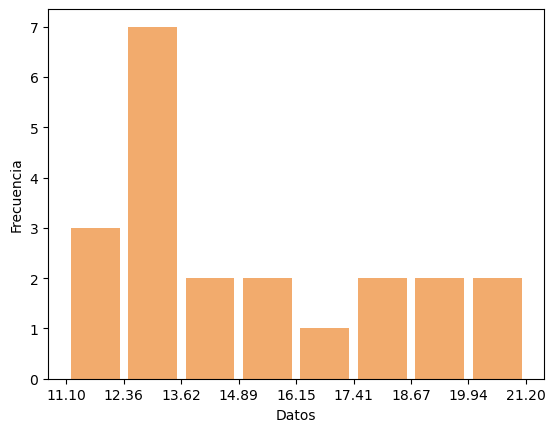
\includegraphics[width=0.4\linewidth]{Figuras/Fig_formalismo_histograma.png}
	\caption{Ejemplo de histograma.}
	\label{Fig_formalismo_histograma}
	\end{figure}

			\SubsubiIt{Ley de los grandes números}

La conexión entre estadística y teoría de la probabilidad se da mediante la \textbf{ley de los grandes números}. Lo que nos dice esta ley es que cuando el número de muestras tiende a infinito, $N\to \infty$, las fracciones relativas tienden a un número fijo que hereda, de toda la dinámica del sistema, ciertas propiedades que no se desvanecen. Este número es la probabilidad, es decir, 
	\begin{equation}
	f_N(x_i) = \frac{n(x_i)}{N}~~~\stackrel{N\to\infty}{\longrightarrow}~~~{p(x_i)}
	\end{equation}
Un punto importante aquí es darnos cuenta de que experimentalmente sólo tenemos acceso a las frecuencias relativas $f_N(x_i)$ para un $N$ grande aunque \textbf{finito}.

Igualmente, nuestro conocimiento de la  media $\overline X$  y la varianza $\sigma_X^2$ siempre es aproximado, y se realiza a través de las medias y varianzas muestrales
\begin{eqnarray}
\overline{A}_N = \sum_i x_i f_N(x_i)~~~&\stackrel{N\to\infty}{\longrightarrow}&~~~ \overline{X}\\
\sigma_{A_N}^2 = \sum_{i} (x_i - \overline{A}_N)^2 f_N(x_i) ~~~&\stackrel{N\to\infty}{\longrightarrow}&~~~ \sigma_X^2
\end{eqnarray}

\begin{mybox_blue}{Nota}
Este es el enfoque \textbf{frecuentista}.
\end{mybox_blue}


			\SubsubiIt{La distribución de Bernouilli}
\begin{mybox_gray2}{}
Una \textbf{variable aleatoria de Bernouilli} $X=(x,p(x))$ tiene dos posibles resultados
\begin{itemize}
	\item \textbf{Exito}:$\to x=1$ con probabilidad $p(1) = p$

	\item \textbf{Fracaso}: $\to x=0$ con probabilidad $p(0) = 1-p$
\end{itemize}
\end{mybox_gray2}

Podemos calcular fácilmente 
	\begin{align}
	\overline X & = \sum_i x_i p_i = 1 \cdot p +0 \cdot (1-p) = p \\
	\sigma^2 & = \sum_i (x-\overline X)^2p_i = (1-p)^2p +(0-p) = p(1-p)
	\end{align}



			\SubsubiIt{La distribución Binomial}

\begin{mybox_gray2}{}
La \textbf{variable aleatoria binomia}l $X = (x,p(x))$ se define como
	\begin{equation}
	x = \text{número de éxitos obtenidos en } n \text{ pruebas de Bernouilli sucesivas}
	\end{equation}
Claramente $x \in (0,1,2,...n)$.

Ahora es muy sencillo obtener la \textbf{probabilidad} de un suceso con $x$ éxitos
	\begin{equation}
	p(x) = \begin{pmatrix}n\\ x\end{pmatrix} p^x (1-p)^{n-x}
	\end{equation}
donde el primer factor tiene en cuenta las posibles ordenaciones en que aparecen $x$ éxitos en $n$ intentos.
\end{mybox_gray2}

Podemos ver esta distribución en la Fig. \ref{Fig_formalismo_dist_binomial}.

Un cálculo un poco más largo permite ver que, ahora
	\begin{align}
	\overline X &=  np\\ \rule{0mm}{7mm}
	\sigma^2 &= n p(1-p)
	\end{align}

	\begin{figure}[H]
	\centering 
	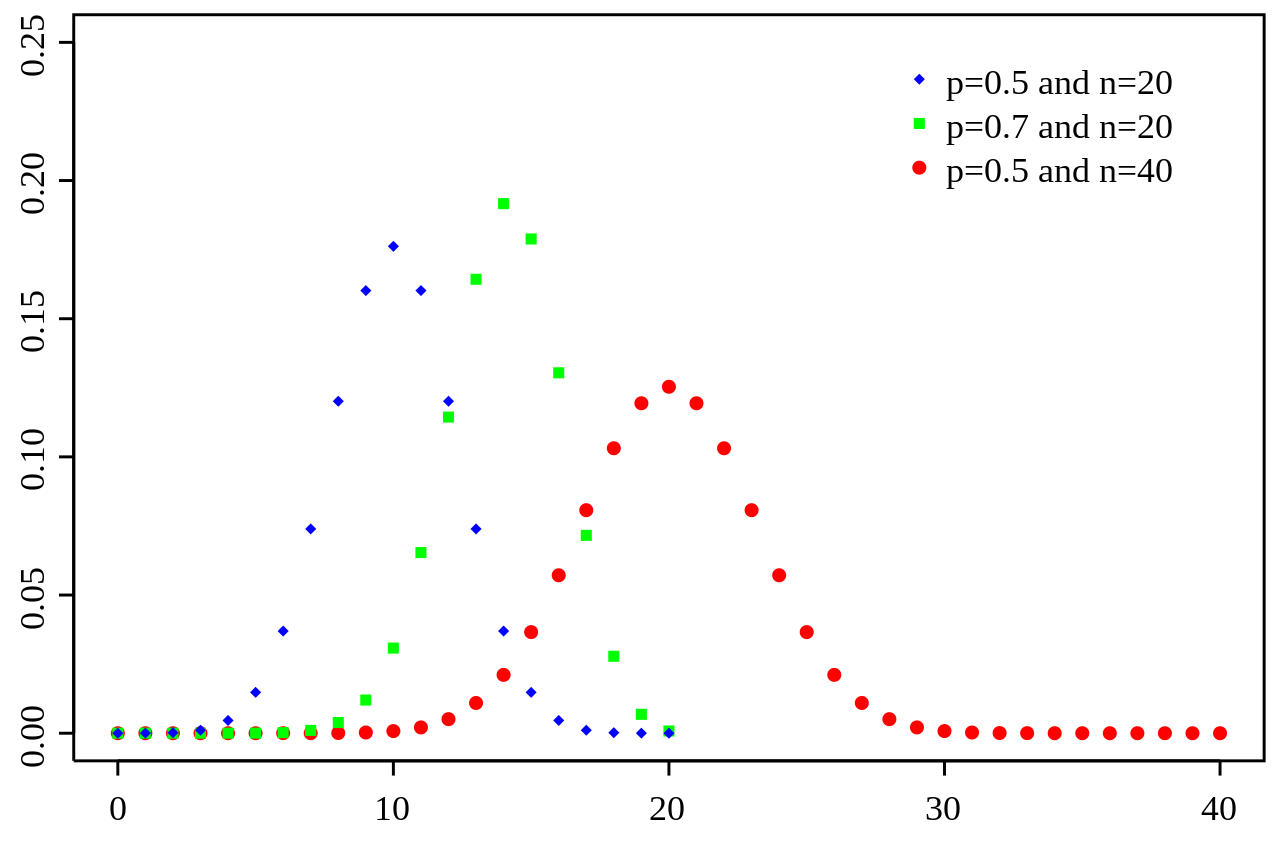
\includegraphics[width=0.4\linewidth]{Figuras/Fig_formalismo_dist_binomial.png}
	\caption{Distribución binomial}
	\label{Fig_formalismo_dist_binomial}
	\end{figure}

			\SubsubiIt{La distribución Normal o Gaussiana}

\begin{mybox_gray2}{}
La \textbf{distribución normal} (o \textbf{gaussiana}) centrada en $\mu$ y con anchura $\sigma$ viene dada por
	\begin{equation}
	p(x) = \frac{1}{\sqrt{2\pi}\sigma} \exp \left({-\frac{(x-\mu)^2}{2\sigma^2}}\right)
	\end{equation}
Nos encontramos ante una variable aleatoria con un espacio muestral continuo $x\in (-\infty,+\infty)$. 
\end{mybox_gray2}

Podemos ver esta distribución en la Fig. \ref{Fig_formalismo_dist_normal}. Tenemos además que

	\begin{align}
	\overline{X} &= \int_{-\infty}^{+\infty} xp(x) dx = \mu \\
	\overline{(x-\overline X)^2} &= \int_{-\infty}^{+\infty} (x-\mu)^2 p(x)dx =\sigma^2
	\end{align}

\begin{figure}[h] \setcounter{subfigure}{0}
\centering
\subfigure[Diferentes valores de $\mu$ y $\sigma$]{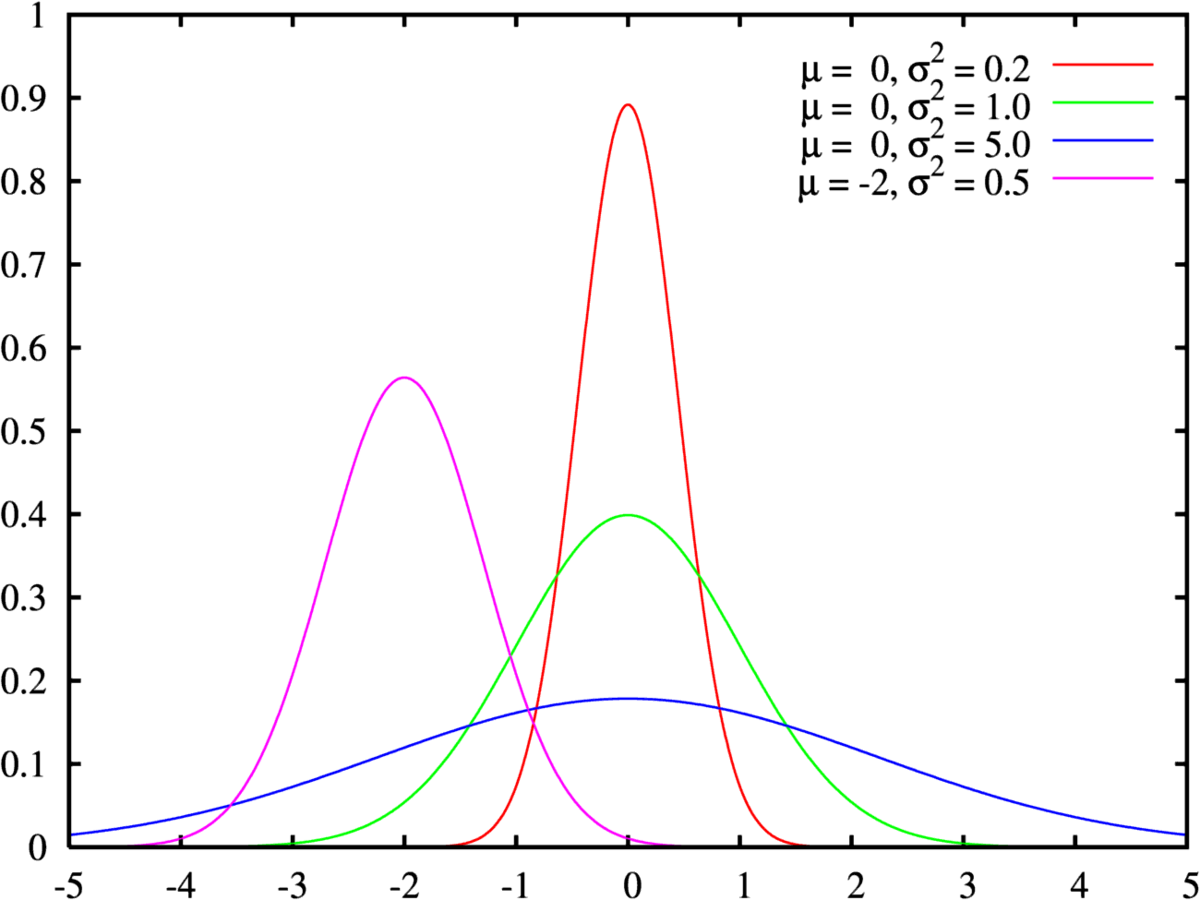
\includegraphics[width=0.4\linewidth]{Figuras/Fig_formalismo_dist_normal.png}}
\hspace{0.5cm}
\subfigure[Distribución de probabilidad en torno a la media]{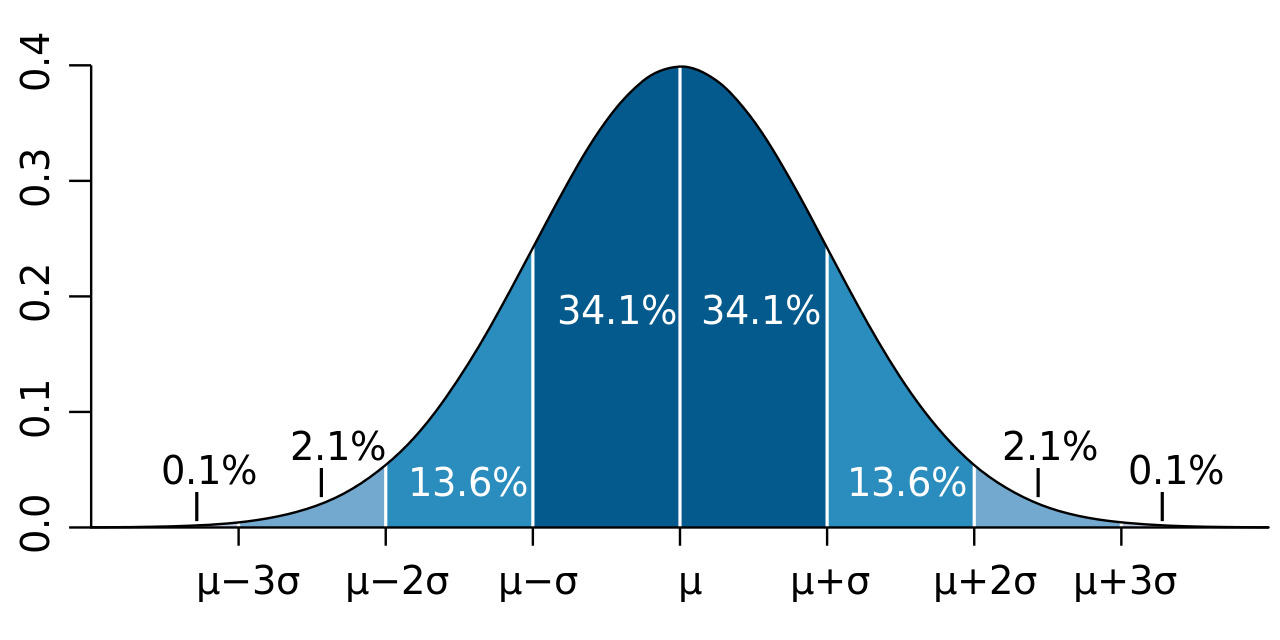
\includegraphics[width=0.45\linewidth]{Figuras/Fig_formalismo_dist_normal_2.png}}
\caption{Distribución normal (o gaussina)}
\label{Fig_formalismo_dist_normal}
\end{figure}





		\subsection{Probabilidades combinadas}

Las probabilidades combinadas son la base de las \textbf{correlaciones}. Es aquí donde la Mecánica Cuántica produce resultados inesperados clásicamente. Esto es porque cantidades que son independientes desde el punto de vista clásico, presentan correlaciones al hacer el experimento. 

Ahora vamos a examinar variables aleatorias formadas por dos espacios muestrales $X$ e $Y$. Dependiendo de la forma en que combinemos la observación de cada una tendremos distintas distribuciones de probabilidad

			\SubsubiIt{Probabilidad combinada}

Una forma de lidiar con las correlaciones es tratar el conjunto de varias variables aleatorias como una sola variable. Esta es la idea detrás de la \textbf{probabilidad combinada}, 

\begin{mybox_gray2}{}
La \textbf{distribución de probabilidad combinada} asocia un número $p(x,y)$ a la probabilidad de observación conjunta de $x$ \textbf{e} $y$. 

De esta forma, tratamos las parejas de eventos  como un solo evento  $a = (x,y)$. Por eso, la condición de normalización ahora es 
	\begin{equation}
	\sum_a p(a) = \sum_{xy} p(x,y) = 1\, .
	\end{equation}
\end{mybox_gray2}

\begin{itemize}
	\item \textbf{Distribución marginal}:
	
	La suma parcial sobre una de las dos variables conduce a sendas \textbf{distribuciones marginales}
		\begin{equation}
		q(x) = \sum_{y} p(x,y) ~~~~~~~~~ \tilde q(y) = \sum_{x} p(x,y)
		\end{equation}

	\item \textbf{Variables independientes}:
	
	Si dos variables aleatorias no presentan \textbf{ninguna correlación}, decimos que son \textbf{independientes}. En este caso las probabilidades combinadas factorizan 
	\begin{equation}
	p(x,y) = p(x) p(y)
	\end{equation}
La distribución de cada variable coincide con la que se deduce de marginalizar la otra
	\begin{equation}
	\sum_y p(x,y) = p(x)~~~~,~~~~\sum_x p(x,y) = p(y)
	\end{equation}

\end{itemize}


			\SubsubiIt{Probabilidad condicionada}

\begin{mybox_gray2}{}
La distribución de \textbf{probabilidad condicionada} $p(X|Y)$ asigna un número $p(x|y)$ a la probabilidad  de encontrar un suceso $X=x$ una vez \textit{sabemos} que $Y=y$ ha sido el resultado de consultar $Y$. 
\end{mybox_gray2}

La manera de acceder experimentalmente a estas distribuciones, es efectuar un muestreo $(a_i,b_i), i=1,...,N$ de valores de $(X,Y)$ y \textit{seleccionar} sólo aquellos sucesos donde $b_i = y$ un valor concreto de $Y$.

\Teorema{ (\textbf{Teorema de Bayes}): Las probabilidades condicionales y combinadas se relacionan de la forma siguiente
	\begin{equation}
	p(x,y) = p(x|y)p(y) = p(y|x) p(x)
	\end{equation}
La segunda igualdad conduce al \textbf{teorema de Bayes}
	\begin{equation}
	p(x|y) = \frac{p(y|x)p(x)}{p(y)}
	\end{equation}
}

		\subsection{Entropía de una una variable aleatoria}

	\Definicion{
	Dada una variable aleatoria $(X,p(X))$ definimos la \textbf{entropía} asociada mediante la expresión
     	\begin{equation}
     	H = -\sum_x p(x)\log p(x)
     	\end{equation}
	}

\begin{itemize}
	\item El signo negativo hace esta expresión positiva, debido a que $\log p(x)\leq 0$.
	
	\item El valor de $H$ está acotado entre $H\in [0,\log(N)]$ donde $N$ es el número de sucesos $x$ posibles
	
	\item Si $p(x_i)=0 \,\,  \forall x_i$ excepto $p(x_0)=1$ para un evento posible $\Rightarrow H=0$
	
	\item Si $p(x_i) = 1/N$ es equiprobable $\Rightarrow H = \log(N)$ y este es el valor máximo. 
	
\end{itemize}

	\begin{mybox_green}{Ejemplo}
	La entropía de la distribución de Bernoulli es 
	\begin{equation}
	H = - p\log p -(1-p)\log (1-p)
	\end{equation}
	
		\begin{figure}[H]
		\centering 
		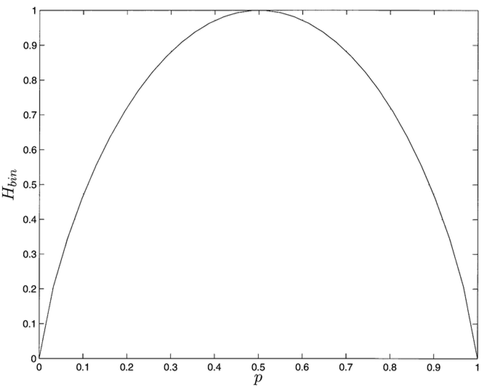
\includegraphics[width=0.5\linewidth]{Figuras/Fig_formalismo_binaryentropy.png}
		\caption{Entropía para una distribución de Bernouilli}
		\label{Fig_formalismo_binaryentropy}
		\end{figure}
	\end{mybox_green}
	
















\chapter{Fundamentos de Mecánica Cuántica} \label{cap_fundamentos}

En este capítulo vamos a hacer una introducción a los fundamentos de la Mecánica Cuántica. Este capitulo se basa en \cite{Curso-JMas}, que a su vez toma como referencias los capítulos 1 y 3 de \cite{Claude}, los capítulos 1, 3 y 4 de \cite{le_bellac_2006} y los capítulos 1-6 de \cite{fayngold2013quantum}. 

Para más información sobre Mecánica Cuántica, se recomienda el famoso libro de Griffits \cite{griffiths_schroeter_2018}.

	\section{Axiomas}


		\subsection{¿Qué es un axioma?}

\begin{mybox_gray2}{}
\textbf{Axioma} es una proposición tan clara y evidente que se admite sin demostración. Aplicado en matemáticas y otras ciencias, es cada uno de los principios indemostrables sobre los que, por medio de un razonamiento deductivo, se construye una teoría.
\end{mybox_gray2}

\begin{mybox_green}{Ejemplo}
Un ejemplo son los axiomas (postulados) de la geometría euclidiana:
\begin{enumerate}
	\item Es posible trazar una línea recta desde cualquier punto a cualquier otro punto.
	\item Es posible prolongar un segmento de recta continuamente en ambas direcciones.
	\item Es posible describir una circunferencia con cualquier centro y cualquier radio.
	\item Es cierto que todos los ángulos rectos son iguales entre sí.
	\item ("Postulado de las paralelas") Es cierto que, si una recta que cae sobre dos rectas hace que el ángulos interiores de un mismo lado sean menores que dos ángulos rectos, las dos rectas, si se producen indefinidamente, se intersecan en aquel lado en el que están los ángulos menores que los dos ángulos rectos.
\end{enumerate}
\end{mybox_green}	
	

		\subsection{Axiomas de la mecánica cuántica}	

La Mecánica Cuántica es una teoría fundamentada en unos pilares axiomáticos cuya selección admite cierta flexibilidad. La más aceptada constituye lo que se denomina la \textbf{interpretación de Copenhagen}. 

		\SubsubiIt{Vector de estado}

\begin{mybox_gray2}{}
En un instante, $t$, la \textbf{máxima información accesible} de un sistema está asociada a un \textbf{vector de estado} $\ket{\psi}$, de norma unidad, $\braket{\psi}{\psi}=1$,  
perteneciente a un espacio de Hilbert $\mathcal{H}$
\end{mybox_gray2}

\begin{itemize}
	\item La dimensión de $\mathcal{H}$ está relacionada con el número de grados de libertad del sistema.

	\item La \textbf{fase global} del vector de estado no contiene información: dos vectores que difieran en una fase global representan al mismo estado ningún experimento permite distinguirlos
	\begin{equation}
	\ket{\psi} \sim \ket{\psi'} =  e^{i\varphi}\ket{\psi} \, .
	\end{equation}

	\item El vector de estado recibe también el nombre de \textbf{función de onda}.
\end{itemize}
		\SubsubiIt{Medidas}

\begin{mybox_gray2}{}
A una magnitud física medible, le está asociado   un operador hermítico  $ A= A^\dagger$ que denominamos \textbf{observable}.
\end{mybox_gray2}

\begin{mybox_gray2}{}
Los resultados de una medición no pueden dar como resultado nada más que uno de los valores propios de $A \Rightarrow \lambda_n$.
\end{mybox_gray2}

\begin{itemize}
	\item Las magnitudes medibles son números reales, de ahí la exigencia de que $A$ deba ser un operador hermítico.
	
	\item La información contenida en $\ket{\psi}$ es \textbf{intrínsecamente probabilística} (no hay variables ocultas). Los resultados de una medida son inciertos, pero $\psi$ codifica una distribución de probabilidad. 
\end{itemize}




		\SubsubiIt{Regla de Born}

\begin{mybox_gray2}{}
La probabilidad de obtener  el autovalor $\lambda_k$ como resultado de una cierta medición, viene dada por la expresión
	\begin{equation}
	p(\lambda_k)~ = ~|\braket{\lambda_k}{\psi}|^2
	\end{equation}
donde $\ket{\lambda_k}$ es el autovector asociado. 
\end{mybox_gray2}

El valor $\braket{\lambda_k}{\psi}$ se denomina \textbf{amplitud}.

La fórmula anterior es cierta cuando el autovalor en cuestion es \textit{no degenerado}. La expresión correcta cuando $\lambda_k$ tiene degeneración $d_k$ es
	\begin{equation} \label{ec_fundamentos_p_para_lambda_degenerado}
	\boxed{p(\lambda_k)~ = ~ \sum_{a=1}^{d_k}|\braket{\lambda^a_k}{\psi}|^2}
	\end{equation}   

		\SubsubiIt{Colapso de la función de ondas}

\begin{mybox_gray2}{}
 Si el resultado de una medida  ha sido  $\lambda_n$, el estado del sistema, inmediatamente después de la medida, viene dado por el vector propio  $\ket{\lambda_n} \in \mathcal{H}$, normalizado $|\braket{\lambda_n}{\lambda_n}|=1$
	\begin{equation}
	\ket{\psi}~\stackrel{\lambda_n}{\Longrightarrow}~ \ket{\lambda_n} 
	\end{equation}
\end{mybox_gray2}

		\SubsubiIt{Evolución en el tiempo}

\begin{mybox_gray2}{}
El cambio  del estado del sistema $\ket{\psi(t)}$ es \textit{determinista} y 
está gobernado por la \textbf{Ecuación de Schrödinger}
	\begin{equation} \label{ec_fundamentos_ec_de_schrodinger}
	i\hbar \frac{\partial\ket{\psi}}{\partial t} = H \ket{\psi} \, ,
	\end{equation}
donde el Hamiltoniano, $H$, es un operador hermítico que \textit{caracteriza} el sistema, y $\hbar$ es una \textit{constante universal} denominada \textbf{constante de Planck}
	\begin{equation}
	\hbar = 1.054 \times 10^{-34} \, J \cdot s
	\end{equation}
\end{mybox_gray2}

\begin{itemize}
	\item $J$=Julio: Unidad en el Sistema Internacional para la Energía
	\item $s=$segundos: Unidad en el Sistema Internacional para el tiempo. 
\end{itemize}
		


	\section{Bases ortogonales}
		
En Mecánica Cuántica especificamos un estado usando las componentes de la expansión del mismo en una base ortogonal. Existen infinitas bases posibles para expresar un vector. ¿Cuál es la mejor base? La respuesta es que depende del proceso que estudiemos. 

Por ejemplo, si el proceso es la \textit{medida} de un cierto observable $A = A^\dagger$, según los postulados el resultado de nuestra medición sólo puede ser uno de los \textit{valores propios} $\lambda_i$
	\begin{equation}
	A \ket{\lambda_k} = \lambda_k \ket{\lambda_k} \,,
	\end{equation}
donde $\ket{\lambda_k}$ son los autovectores $k = 1,2,\dots$. Estos autovectores forman una base ortonormal (ver Ecs. (\ref{ec_op_hermitico_autovec_ortonorm}) y (\ref{ec_op_hermitico_autovec_ortogonal})). Esta es la base natural adaptaba al proceso de medida de $A$. En particular, para conocer con que probabilidad se producirá cada resultado, expandiremos el estado de la forma
	\begin{equation}
	\ket{\psi} = \sum_{i=1}^{N} a_i \ket{\lambda_i} \, .
	\end{equation}
El axioma III (regla de Born) afirma que la \textit{probabilidad de aparición} del resultado $\lambda_i$ es precisamente
	\begin{equation}
	p(\lambda_i) = | \braket{\lambda_i}{\psi} |^2 = |a_i|^2 \, .
	\end{equation}

La forma de tener acceso experimental a los números $p(\lambda_i)$ es mediante la repetición estadística. Si efectuamos la medida un número $n$ de veces con $n \rightarrow \infty$, y contamos la frecuencia de aparición de los distintos $\lambda_i$, esto es 
	\begin{equation}
	p(\lambda_i) \approx \frac{n(\lambda_i)}{n} \, ,
	\end{equation}
en el límite $n \rightarrow \infty$ dicha frecuencia experimental convergerá a la probabilidad teórica
	\begin{equation}
	\lim_{n \rightarrow \infty} \frac{n(\lambda_i)}{n} = p(\lambda_i) = | a_i |^2 \, .
	\end{equation}
Vemos que, \textit{mediante la repetición estadística, solamente podemos recuperar el módulo de las amplitudes}
	\begin{equation}
	|a_i| = \lim_{n \rightarrow \infty} \sqrt{\frac{n(\lambda_i)}{n}}
	\end{equation}

	
	\Ejercicio{Generalizar las expresiones anteriores al caso en que los autovalores $\lambda_k$ puedan ser $d_k$ veces degenerados.
	}

	\section{Medidas Estadísticas}
	
		\subsection{Valor esperado}

Vamos a reescribir la Ec. (\ref{ec_fundamentos_p_para_lambda_degenerado})
\begin{eqnarray} \label{ec_fundamentos_p_para_lambda_degenerado_proyector}
p(\lambda_k)~ 
&=& ~ \sum_{a=1}^{d_k}|\braket{\lambda^a_k}{\psi}|^2 
 = \sum_{a=1}^{d_k} \braket{\psi}{\lambda^a_k}\braket{\lambda^a_k}{\psi}  
 =\bra{\psi}\left(\sum_{a=1}^{d_k}\ketbra{\lambda^a_k}{\lambda^a_k}\right) \ket{\psi}\nonumber\\
&=&  \bra{\psi}P_k\ket{\psi} 
\end{eqnarray}    
donde 
	\begin{equation}
	\boxed{P_k = \sum_{a=1}^{d_k} \ket{\lambda^a_k}\bra{\lambda^a_k}}
	\end{equation}
es el \textbf{proyector sobre el subespacio propio} (ver Ec. (\ref{ec_formalismo_proyec_subespacio_propio})).

Por el \textbf{valor esperado} $\langle A\rangle$ del \textit{observable} $A$ en el estado $\ket{\psi}$, entendemos el \textit{valor medio} de la variable aleatoria $\lambda_n$ obtenida por el método descrito. 
\begin{eqnarray}
\langle A\rangle 
	&= &  \sum_k \lambda_k p(\lambda_k)
     =  \sum_k \lambda_k \bra{\psi}P_k\ket{\psi}  \nonumber \\
	&=& \bra{\psi}\left(\sum_k \lambda_k P_k  \right) \ket{\psi} 
\end{eqnarray}
Reconocemos entre paréntesis la descomposición espectral de $A$. Llegamos así a la siguiente expresión para el valor esperado de un observable $A$ en un estado $\ket{\psi}$:
	
	\Teorema{ El \textbf{valor esperado de un operador} es
		\begin{equation}
		\langle A \rangle=\bra{\psi}A \ket{\psi}
		\end{equation}
	}

\begin{itemize}
	\item En particular, las probabilidades mismas se pueden expresar como \textit{valores esperados del proyector asociado}
	\begin{equation}
	p(\lambda_k ) =  \bra{\psi}P_k\ket{\psi} = \langle P_k\rangle 
	\end{equation}
	
	\item El valor esperado de un observable en uno de sus autoestados coincide con el autovalor asociado
	\begin{equation}
	\bra{\lambda_i}A \ket{\lambda_i} = \bra{\lambda_i}\lambda_i \ket{\lambda_i}  = \lambda_i \braket{\lambda_i}{\lambda_i} = \lambda_i
	\end{equation}

\end{itemize}

El espectro de un observable está formado por números reales que podemos ordenar $\lambda_{min}<...<\lambda_{max}$.

	\Teorema{
	El valor esperado de un observable $A$ está acotado entre sus valores propios mínimo y máximo
	\begin{equation}
	\lambda_{min} \leq \bra{\psi}A\ket{\psi} \leq \lambda_{max}
	\end{equation}
	y las desigualdades anteriores se saturan en los autoestados correspondientes
	}


		\subsection{Varianza y Desviación estándar}

\begin{mybox_gray2}{}
La \textbf{varianza} es la media de la desviación cuadrática de la variable aleatoria $(\lambda,p(\lambda))$ es decir 
	\begin{equation}
	~~\sigma ^2 = \overline{(\lambda_i-\bar\lambda_i)^2}= \overline{\lambda^2} - \overline{\lambda}^2
	\end{equation}
de aquí se sigue, para la \textbf{desviación estándar}
	\begin{equation}
	\sigma = \sqrt{\bra{\psi}A^2\ket{\psi} - \bra{\psi} A\ket{\psi}^2}
	\end{equation}
\end{mybox_gray2}


	
	\section{Evolución temporal}



		\SubsubiIt{Ecuación de Schrödinger}

El estado de un sistema $\ket{\psi(t)}$ posee la máxima información instantánea accesible de un sistema, es decir, a un tiempo dado $t$. Dado $\ket{\psi(t_0)}$ en un instante inicial $t_0$, la evolución posterior obedece a la  ecuación diferencial de Schrödinger
	\begin{equation} \label{ec_fundamentos_ec_de_schrodinger_con_t}
	i \hbar \frac{d}{d t}\ket{\psi(t)} = H(t) \ket{\psi(t)} \, .
	\end{equation}

\begin{mybox_blue}{Nota}
\begin{itemize}
	\item El operador Hamiltoniano $H(t)$  contiene toda la información sobre la dinámica del sistema.
	\item Hemos enfatizado el hecho de que, en el caso más general, $H(t)$ puede depender del tiempo.
\end{itemize}
\end{mybox_blue}

		\SubsubiIt{Conservación de la probabilidad}

La hermiticidad de $H$ se relaciona directamente con la interpretación probabilística de $\ket{\psi}$. Efectivamente, en \textit{la evolución temporal se conserva la norma del vector de estado}
\begin{eqnarray}
\frac{d}{dt}\braket{\psi(t)}{\psi(t)} &=& \left(\rule{0mm}{3mm}\frac{d}{dt}\bra{\psi(t)}\right)\ket{\psi(t)} + 
\bra{\psi(t)}\left(\frac{d}{dt}\ket{\psi(t)} \right)\nonumber\\
&=& \left(\bra{\psi(t)}\frac{i}{\hbar}H^\dagger\right)\ket{\psi(t)} + \bra{\psi(t)}\left(-\frac{i}{\hbar}H\ket{\psi(t)} \right) \\
&=&\frac{i}{\hbar} \bra{\psi(t)}(H^\dagger - H)\ket{\psi(t)} = 0 \nonumber
\end{eqnarray}
Esto implica que la norma de $\ket{\psi(t)}$ se conserva $\Rightarrow 1 = \|\ket{\psi(0)}\| =\|\ket{\psi(t)}\|$


		\SubsubiIt{Operador de evolución}

La conservación de la norma implica que la evolución $\|\ket{\psi(0)\|} =\|\ket{\psi(t)}\|$ es un \textit{proceso unitario}. En otras palabras, debe existir un operador unitario 
	\begin{equation}
	U(t,t_0)^{-1}= U(t,t_0)^\dagger 
	\end{equation}
que lleve el estado inicial al actual a tiempo $t$
	\begin{equation}
	 U(t,t_0): \ket{\psi(t_0)}~~ \to~~ \rule{0mm}{3.5mm} \ket{\psi(t)} = U(t,t_0)\ket{\psi(t_0)}
	\end{equation}

\begin{mybox_blue}{Propiedades de ${U(t,t_0)}$}
El operador de evolución satisface las siguientes propiedades
\begin{itemize}
	\item $U(t_0,t_0) = I$ \, .
	\item transitividad:  $U(t,t_1)U(t_1,t_0)= U(t,t_0)$
	\item invertibilidad: $U(t,t_0)^{-1} = U(t_0,t)$
\end{itemize}
\end{mybox_blue}

Evidentemente, el operador de evolución debe estar relacionado con el Hamiltoniano, que es quien gobierna la dinámica. Veamos a ver que hay una ecuación de Schrödinger también para el operador de evolución

	\Teorema{
	El operador de evolución satisface la siguiente ecuación de evolución
		\begin{equation}
		i \hbar \frac{d}{dt}U(t,t_0) = H(t)\, U(t,t_0)
		\end{equation}
	}
\begin{proof}
Tomando la derivada temporal de la ecuación $\ket{\psi(t)} = U(t,t_0)\ket{\psi(t_0)}$, que define $U(t,t_0)$, tenemos para cada miembro

\begin{eqnarray}
i \hbar \frac{d}{dt}\ket{\psi(t)} &~=~&   H(t)\ket{\psi(t)} =  H(t)U(t,t_0)\ket{\psi(t_0)}  \nonumber\\
i \hbar \frac{d}{dt}\ket{\psi(t)} &~=~& i \hbar \frac{d}{dt}U(t,t_0)\ket{\psi(t_0)} = i \hbar \left(\frac{d}{dt}U(t,t_0)\right)\ket{\psi(t_0)}
\end{eqnarray}
Igualando ambas expresiones, y teniendo en cuanto que $\ket{\psi_0}$ es arbitrario, obtenemos la ecuación deseada.
\end{proof}



		\SubsubiIt{Caso de $H$ independiente del tiempo}

Cuando $H$ no depende del tiempo podemos dar una expresión analítica para el operador de evolución
	\Teorema{
	Para un hamiltoniano $H$ independiente del tiempo, el operador de evolución $U(t,t_0)$ es
		\begin{equation}
		U(t,t_0) = \exp\left({-\frac{i}{\hbar} (t-t_0)H}\right)
		\end{equation}
	}
	\begin{proof}
	Basta con demostrar que se satisface la ecuación de evolución y la condición de contorno

\begin{eqnarray}
\frac{d}{dt}U(t,t_0) &=& \frac{d}{dt} \exp\left({-\frac{i}{\hbar} (t-t_0)H}\right)
    \nonumber\\ \rule{0mm}{6mm}
   &=& \frac{d}{dt}\left( I +(t-t_0)\left(-\frac{i}{\hbar} H\right) + \frac{1}{2!} 
    (t-t_0)^2\left(-\frac{i}{\hbar} H\right)^2  + ...\right) \nonumber\\ \rule{0mm}{6mm}
    &=& 0 +  \left(-\frac{i}{\hbar} H\right) +  (t-t_0)\left(-\frac{i}{\hbar} H\right)^2  + ... \nonumber\\ \rule{0mm}{6mm}
&=&  \left(-\frac{i}{\hbar} H\right)\left( I + (t-t_0) \left(-\frac{i}{\hbar} H\right) + ...\right)
  \nonumber \\ \rule{0mm}{6mm} 
&=& \left(-\frac{i}{\hbar} H\right) \exp\left({-\frac{i}{\hbar} (t-t_0)H}\right)    \nonumber\\ \rule{0mm}{6mm}
&=& -\frac{i}{\hbar} H \,  U(t,t_0)
\end{eqnarray}
Además
	\begin{equation}
	U(t_0,t_0) =  \exp\left({-\frac{i}{\hbar} (t_0-t_0)H}\right)=\exp(0) = I
	\end{equation}
	\end{proof}
	
	\begin{mybox_blue}{Nota}
	La cantidad ${-\frac{i}{\hbar} (t-t_0) H }$ es adimensional
	\begin{equation}
	\frac{1}{\hbox{J}\cdot \hbox{s}}\hbox{s}\cdot\hbox{J} = 1
	\end{equation}
	Es decir, es un número puro. Por eso podemos exponenciarla. El operador de evolución $U(t,t_0)$ es, por tanto, también, una magnitud adimensional.
	\end{mybox_blue}

		\SubsubiIt{Evolución en la base de eutoestados de $H$}

Sea $\{\ket{n}\}$ una base de autoestados de $H \, \Rightarrow \,H \ket{n} = E_n \ket{n}$, $n=1,..,N$. En esta base $H$ es una matriz $H_{mn}$ diagonal 
	\begin{equation}
	H_{mn} =  \begin{bmatrix} E_0 &  & & \\  & E_1 &  & \\ & & \ddots & \\ & & & \end{bmatrix} =E_m \delta_{mn} \, .
	\end{equation}
Entonces la matriz de evolución es también diagonal 
	\begin{equation}
	U_{mn} = \exp\left(-\frac{i}{\hbar}t H_{mn}\right) = 
 \begin{bmatrix} e^{-\frac{i}{\hbar}t E_0} &  & & \\  & e^{-\frac{i}{\hbar} t E_1}  &  & \\ & & \ddots & \\ & & & \end{bmatrix} = e^{-\frac{i}{\hbar} t  E_m }\delta_{mn} \, .
	\end{equation}

En conclusión:
	\begin{itemize}
	\item La evolución temporal de un autoestado de la energía es trivial (es una fase global)
	\begin{equation}
	U(t,0)\ket{n} = e^{-\frac{i}{\hbar} t E_n} \ket{n}\, 
	\end{equation}
	Es decir, un autoestado del hamiltoniano es un \textbf{estado estacionario}. Si nuestro sistema está en un autoestado del hamiltoniano, este no cambiará con el tiempo.

	\item Esta fase deja de ser trivial cuando afecta a una combinación lineal. La forma más eficaz de calcular la evolución de un estado arbitrario es expresarla en la base $\{\ket{n}\}$. Es decir, si a $t=0$
	\begin{equation}
	\ket{\psi(t=0)} = \sum_n c_n \ket{n} \, 
	\end{equation}
entonces, a tiempo $t$ 
	\begin{equation}
	\ket{\psi(t)} = \sum_n c_n e^{-\frac{i}{\hbar}E_nt} \ket{n} \, .
	\end{equation}
En esta base, la evolución temporal lo que hace es que las fases relativas de los autoestados evolucionen a velocidades diferentes.

	\end{itemize}

		
	    \begin{mybox_orange}{Jupyter Notebook: 00-Fundamentos\_MC\_evolucion\_temporal}
    Puede verse el Notebook \textit{00-Fundamentos\_MC\_evolucion\_temporal}. En el se muestran dos ejercicios resueltos sobre como calcular la evolución temporal en python.
    Qiskit en Python.
    \end{mybox_orange}
		
		
		
	\section{Estados Mezcla y Matriz Densidad}



		\subsection{Estado puro y mezcla}

Hasta ahora hemos estado estudiando casos \textbf{ideales}, donde los estados que tenemos son \textit{perfectos}, en el sentido de que tenemos el estado que creemos tener con una probabilidad del 100\%. Esto en la vida real no es así. Cuando intentamos generar un estado cuántico, nunca vamos a generar estos estados perfectos, pues nuestros aparatos no son perfectos y nunca lo serán. Todo aparato lleva asociada una \textbf{incertidumbre}, es decir, una probabilidad de error.

A estos estados \textit{perfectos} se los denomina \textbf{estados puros}, mientras que al resto de estados se los denomina \textbf{estados mezcla}.

			\SubsubiIt{Estos puros}
			
Si sabemos \textit{con seguridad} que el  sistema se encuentra en un estado $\ket{\psi}\in \mathcal{H}$ \textit{toda la incertidumbre} que queda es cuántica.

	\begin{mybox_gray2}{}
	\textbf{Estado puro}:
	
	Si con \textit{certeza total} podemos afirmar que el estado de un sistema está descrito por un vector $\ket{\psi}\in \mathcal{H}$ decimos que nuestro sistema se encuentra en un \textbf{estado puro}.
	\end{mybox_gray2}


Tomemos un estado \textbf{superposición} 
	\begin{equation}
	\ket{\psi} = a\ket{0} + b\ket{1}
	\end{equation}
con $a,b \neq 0$. 
La probabilidad de medir el estado $\ket{0}$ será positiva
	\begin{equation}
	p(0) = |\braket{0}{\psi}|^2  = 
\left\vert\bra{0}\big(a\ket{0}+b\ket{1}\big)\right\vert^2=\left\vert a\braket{0}{0}+b \braket{0}{1}\right\vert^2 = |a|^2
	\end{equation}
la de medir el estado $\ket{1}$ también
	\begin{equation}
	p(1) = |\braket{1}{\psi}|^2  = \left\vert\bra{1}\big(a\ket{0}+b\ket{1}\big)\right\vert^2 =\left\vert a\braket{1}{0}+b \braket{1}{1}\right\vert^2= |b|^2
	\end{equation}
y la de medir el estado $\ket{+} =  \frac{1}{\sqrt{2}}(\ket{0}+\ket{1})$ será
\begin{eqnarray}
p(+)&=&|\braket{+}{\psi}|^2 =  \frac{1}{2}\left\vert\big(\bra{0}+ \bra{1}\big)\big(a\ket{0}+b\ket{1}\big)\right\vert^2 = \frac{1}{2}\left\vert\big(a\braket{0}{0}+b\braket{1}{1}\big)
\right\vert^2  \nonumber \\
&=&\frac{1}{2}|a+b|^2  = \frac{1}{2}(a+b)(a^* + b^*) 
\\
&=& \frac{1}{2}\left(\rule{0mm}{4mm} |a|^2 + |b|^2 + 2{\rm Re}(ab^*) \right) \nonumber
\end{eqnarray}    
El término que no tiene signo definido $2{\rm Re}(ab^*)$ se denomina \textit{interferencia}. 
 Es el responsable de que $p(+)=0$ se pueda anular aun cuando $a,b\neq 0$. Concretamente cuando $a=1=-b$
	\begin{equation}
	\ket{\psi}=   \frac{1}{\sqrt{2}}(\ket{0}-\ket{1}) = \ket{-}
	\end{equation}
y los estados son ortogonales $|\braket{\psi}{+}|^2=|\braket{-}{+}|^2= p(\ket{-}\to\ket{+})=0$, obteniendo $p(+)=0$.

			\SubsubiIt{Estados mezcla}
			
¿Qué ocurre si no podemos tener la certeza de que el estado que describe el sistema sea $\ket{\psi}$?  

Por ejemplo: supongamos que, 
\begin{itemize}
	\item a la salida de un polarizador de Stern Gerlach, encontramos que el estado es $\ket{+}$, 
	\item pero la fiabilidad nominal de dicho aparato es del 90\%. 
	\item Eso quiere decir que, con un 10\% de probabilidad, el estado emergente ha sido, en realidad, $\ket{-}$.
\end{itemize}
Nuestro polarizador se comporta como una \textit{variable aleatoria} $ \{\{\ket{+},0.9\},\{\ket{-},0.1\}\}$ de la que obtendremos, cada vez, un estado u otro con distinta probabilidad. 

\begin{mybox_blue}{Nota}
Véase que esta incertidumbre debida al error del polarizador que genera el estado es clásica, no cuántica.
\end{mybox_blue}

\begin{mybox_gray2}{}
\textbf{Estados mezcla}:

En la situación más general, un  sistema estará en un \textbf{estado mezcla} asociado a una variable aleatoria
	\begin{equation}
	\{\ket{\psi_\alpha},p_\alpha\}
	\end{equation}
que indica que, con probabilidad $p_\alpha$,  el estado real del sistema es $\ket{\psi_\alpha}$
\end{mybox_gray2}

\begin{itemize}
	\item Un estado mezcla no es un vector en el espacio de Hilbert, sino que es una variable aleatoria donde el espacio muestral son vectores en el espacio de Hilbert.

	\item Es importante recalcar que las probabilidades $p_\alpha \in  \mathbb{R}$ son incertidumbres clásicas, y por tanto $p_k \in \lc 0,1 \rc$, $\sum_\alpha p_\alpha = 1$.

	\item El estado mixto contiene al estado puro como caso particular en el que para un cierto valor $\alpha = i$, tenemos $p_i = 1$ y el resto son cero. 
\end{itemize}


		\subsection{Operador densidad}

El formalismo matemático que nos permite lidiar con los estados mezcla pasa por usar la \textbf{matriz densidad}.

Supongamos que a nuestro sistema le podemos asignar un estado mixto $\{\ket{\psi_\alpha},p_\alpha\}$. La probabilidad, $p(\lambda_n)$, de encontrar un autovector $\ket{\lambda_n}$ como resultado de la medida de un observable $A$, debe ser la \textit{suma ponderada} de probabilidades  de esa medida en cada uno de los estados $\ket{\psi_\alpha}$
	\begin{equation} \label{ec_fundamentos_op_dens_prob}
	\begin{array}{rcl} 
p(\lambda_n) &=& \sum_\alpha p_\alpha |\braket{\lambda_n}{\psi_\alpha}|^2  =  \sum_\alpha p_\alpha \braket{\lambda_n}{\psi_\alpha}\braket{\psi_\alpha}{\lambda_n} \\ \rule{0mm}{6mm}
&=& \bra{\lambda_n}\left(\rule{0mm}{6mm}\sum_\alpha p_\alpha \ket{\psi_\alpha}\bra{\psi_\alpha}\right)\ket{\lambda_n} \\
&\equiv&\bra{\lambda_n}\rho\ket{\lambda_n}\\
\end{array}
	\end{equation}
El resultado anterior muestra la aparición en escena de un \textit{nuevo operador} formado con los datos del colectivo aleatorio $\{\ket{\psi_\alpha},p_\alpha\}$  
	\begin{equation} \label{ec_fundamentos_operador_densidad_diag}
	\boxed{\rho = \sum_\alpha p_\alpha \ketbra{\psi_\alpha}{\psi_\alpha} = \sum_\alpha p_\alpha P_\alpha}
	\end{equation}
$\rho ~$ se denomina \textbf{matriz densidad} y consiste en una suma ponderada de proyectores sobre cada uno de los subespacios generados por los estados posibles. Este es el objeto matemático que caracteriza un estado mezcla. 

En particular, como acabamos de ver, la probabilidad de medir el autovalor $\lambda$ es el \textit{valor esperado} del operador densidad en dicho estado
	\begin{equation}
	\boxed{p(\lambda_n) =\langle \rho \rangle_{\ket{\lambda_n}} = \bra{\lambda_n }\rho\ket{\lambda_n}}
	\end{equation}

\begin{mybox_gray2}{}
\textbf{Operador densidad}:

Un operador, $\rho$, podrá ser el operador densidad de un sistema si cumple los siguientes requisitos    
\begin{itemize}
	\item es hermítico $\rho = \rho^\dagger$
	\item es semidefinido positivo
	\item tiene traza unidad ${\rm tr }\rho = 1$ 
\end{itemize}

\end{mybox_gray2}

Claramente la expresión dada anteriormente cumple con todos estos requisitos. 
\begin{itemize}
	\item Hermiticidad: se ve gracias a que los $p_\alpha$ son probabilidades (números reales)
	\begin{equation}
	\rho^\dagger = \left(\sum_\alpha p_\alpha \ketbra{\psi_\alpha}{\psi_\alpha}\right)^\dagger = 
\sum_\alpha p^*_\alpha \ketbra{\psi_\alpha}{\psi_\alpha} = \rho
	\end{equation}

	\item De hecho escrito en esta base, la matriz que representa $\rho$ es diagonal
	\begin{equation}
	\rho = \begin{bmatrix} p_1& 0 & ... & 0 \\ 0 & p_2 & ... & 0 \\ & &\vdots  & \\ 0 & 0 & \cdots & p_n  
\end{bmatrix}
	\end{equation}
Por tanto los números $p_\alpha\geq 0$ son los autovalores, que son no-negativos, lo cuál caracteriza un operador semidefinido positivo. 

	\item Finalmente la traza es la unidad debido a que $p_\alpha$ son probabilidades
	\begin{equation}
	{\rm Tr}\, \rho = \sum_\alpha p_\alpha = 1
	\end{equation}

\end{itemize}

\begin{mybox_blue}{Nota}
Es importante darse cuenta de que un estado mezcla \textbf{no se puede escribir como un vector de estado}. Solo los estados puros pueden ser escritos así. 
\vspace{0.3cm}

Por ejemplo, en el caso que veíamos antes de un polarizador que generaba el estado $\ket{+}$ con una probabilidad del 90\%, este se comportaba como una variable aleatoria $ \{\{\ket{+},0.9\},\{\ket{-},0.1\}\}$. El estado que sale de este polarizador es un estado mezcla que se puede expresar con siguiente matriz densidad
	\begin{equation}
	\rho = \Lc 0.9 \ketbra{+}{+}\Rc + \Lc 0.1 \ketbra{-}{-} \Rc
	\end{equation}
Este estado \textbf{no es el mismo} que el estado puro
	\begin{equation}
	\ket{\psi} = \sqrt{0.9} \ket{+} + \sqrt{0.1} \ket{-}
	\end{equation}
Es más, podemos escribir la matriz densidad de este segundo estado para ver que es diferente:
	\begin{align}
	\rho_{\ket{\psi}} 
	& =	\ketbra{\psi}{\psi} 
	  = \lp \sqrt{0.9} \ket{+} + \sqrt{0.1} \ket{-} \rp 
		\lp \sqrt{0.9} \bra{+} + \sqrt{0.1} \bra{-} \rp \\
	& = \Lc 0.9 \ketbra{+}{+} \Rc + \Lc 0.1 \ketbra{-}{-} \Rc + \Lc \sqrt{0.9}\sqrt{0.1} \ketbra{+}{-} \Rc  + \Lc \sqrt{0.9}\sqrt{0.1} \ketbra{-}{+} \Rc
	\end{align}
\end{mybox_blue}


\begin{mybox_blue}{Nota}
La matriz densidad de un estado mezcla \textbf{no tiene porque ser diagonal}. La Ec. (\ref{ec_fundamentos_operador_densidad_diag}) es simplemente el caso en el que estamos en una base donde la matriz es diagonal.
\end{mybox_blue}

			\SubsubiIt{Matriz densidad de un estado puro}

La matriz densidad es un formalismo más general que el del vector estado, que sólo se aplica en el caso de estados puros. En efecto, la matriz densidad asociada a un estado puro $\ket{\psi_0}$ se obtiene haciendo todas las probabilidades $p_{\alpha\neq 0}=0$ y $p_{0} = 1$. Entonces el colectivo $\{\ket{\psi_0},p_0=1\}$ tiene asociado el operador
	\begin{equation}
	\rho = \ketbra{\psi_0}{\psi_0} = \begin{bmatrix}1 &  & \\ & 0 & \\ & & \ddots  \end{bmatrix}
	\end{equation}
Es evidente que esta expresión cumple, a mayores, la propiedad que caracteriza a un \textbf{proyector}
	\begin{equation}
	\rho^2 = \rho
	\end{equation}
y esto es una ecuación que \textit{sólo verifican las matrices densidad asociadas a estados puros}.

\textbf{Por el contrario}, para un estado mezcla podemos ver que $\rho^2 \neq \rho$
	\begin{equation}
	\rho^2  = \sum_\alpha p_\alpha^2 \ketbra{\psi_\alpha}{\psi_\alpha} \neq  \sum_\alpha p_\alpha \ketbra{\psi_\alpha}{\psi_\alpha} = \rho
	\end{equation}

Podemos extraer esta información de forma \textit{independiente de la base} usando la función traza  ${\rm Tr}$
\begin{itemize}
	\item Si $\ket{\psi_\alpha}$ son vectores ortonormales,  ${\rm Tr } \rho = \sum p_\alpha = 1$ pero  ${\rm Tr }\rho^2 = \sum_\alpha p_\alpha^2\leq 1$
	
	\item La igualdad ${\rm Tr} \rho^2=1$ sólo se producirá si  $p_\alpha = 1$ para un solo $\alpha$. 
\end{itemize}

	\Teorema{
	Un estado  $\rho$ será \textit{puro} (\textit{mezcla}) sí y solo sí ${\rm Tr } \rho^2 = 1~~
 ({\rm Tr } \rho^2 <1)$  
	}


			\SubsubiIt{Estado máximalmente mezclado}

En el extremo opuesto de un estado puro, encontramos un estado \textbf{maximalmente mezclado}, en el cual \textit{todos} los proyectores aparecen de manera equiprobable $\{\ket{\psi_\alpha},p_\alpha = \frac{1}{d}\}, \alpha = 1,...,d$
	\begin{equation}
	\rho = \sum_{\alpha=1}^d \frac{1}{d} \ket{\psi_\alpha}\bra{\psi_\alpha} = \frac{1}{d} I = \begin{bmatrix}\frac{1}{d} &  & & \\ & \frac{1}{d} &  &\\ & & &\ddots & \\ & & & & \frac{1}{d} \end{bmatrix}
	\end{equation}
Por tanto, es una matriz diagonal proporcional a la identidad.


			\SubsubiIt{Estado mezcla parcial}

Entre los dos extremos mencionados anteriormente, estado puro y estado maximalmente mezclado, se sitúa cualquier estado $\rho$ genérico. Si escribimos
	\begin{equation}
	\rho = \sum_{\alpha} p_\alpha \ketbra{\psi_\alpha}{\psi_\alpha}
	\end{equation}
el grado de mezcla es proporcional a la uniformidad en la distribución de valores $p_\alpha$. 



			\SubsubiIt{Estado de Gibbs}


Un caso muy importante de mezcla parcial es el \textbf{estado de Gibbs}, que describe un sistema cuando alcanza el \textit{equilibrio término a una temperatura }$T$. En este caso, los estados $\{\ket{\psi_\alpha}= \ket{E_\alpha}\}$ son la \textit{base de autoestados del operador Hamiltoniano},
	\begin{equation}
	H\ket{E_\alpha} = E_\alpha \ket{E_\alpha}
	\end{equation}
y los autovalores $E_\alpha$, con $\alpha = 1,2...d$, son los \textit{niveles de energía} del sistema. 

Cuando un sistema se encuentra en contacto con un baño térmico a temperatura $T$ el estado de energía no está bien definido, sino que es una mezcla denominada \textbf{colectivo canónico}
	\begin{equation}
	\left\{\rule{0mm}{5mm}\ket{E_\alpha}, p_\alpha = e^{-E_\alpha/k_BT}\right\}
	\end{equation}
Los coeficientes $p_\alpha = e^{-E_\alpha/k_BT}$ se denominan \textit{coeficientes de Boltzmann}  codifican la probabilidad  de hallarse en el estado (nivel de energía) $\ket{E_\alpha}$. 

La matriz densidad que describe el estado de este sistema es el denominado \textbf{estado de Gibbs}
	\begin{equation}
	\rho(T) = \frac{1}{Z}\sum_{\alpha=1}^d e^{-E_\alpha/k_BT} \ket{E_\alpha}\bra{E_\alpha} = \frac{1}{Z} \begin{bmatrix}e^{-E_0/k_BT}&  & \\ & e^{-E_1/k_BT} & \\ &  &\ddots  \end{bmatrix} \, ,
	\end{equation}
donde $k_B$ es la constante de Bolzmann, y  $Z =\sum_\alpha e^{-E_\alpha/k_BT}$ es la normalización necesaria para que ${\rm tr}\rho(T) = 1$. La \textbf{energía del sistema} a cada temperatura, vendrá dada por un promedio sobre todos los autoestados pesados por la matriz densidad a dicha temperatura
	\begin{equation}
	\langle E \rangle_T = {\rm tr} (\rho(T) H)
	\end{equation}

\begin{mybox_blue}{Nota: autoestados del Hamiltoniano}
Como ya comentamos, un autoestado de un operador es un estado donde el observable (operador) toma un valor concreto (el autovalor). Los autoestados del operador hamiltoniano son especiales, pues son los \textbf{niveles de energía}. Es decir, los autovalores son las \textbf{energías}. 
\end{mybox_blue}

	\Ejercicio{
	Probar  que recuperamos los casos puro y maximalmente mezclado en los límites siguientes
	\begin{itemize}
		\item $\rho(T=0) = \ketbra{E_0}{E_0}$
		\item $\rho(T=\infty) = \frac{1}{d} I$
	\end{itemize}
	}

	\Ejercicio{
	Genera aleatoriamente un estado de Gibbs a temperatura $T$ y grafica los valores de $p_\alpha(T)$
    para distintos valores de $T$ (toma $k_B=1$).
	}
	
			\SubsubiIt{Entropía de Von Neumann}

La entropía de Von Neumann $S(\rho)$ es una medida del \textit{grado de mezcla} que hay en una matriz densidad. Se define  como sigue
	\begin{equation}
	S(\rho) = -{\rm tr} (\rho \log \rho )\, .
	\end{equation}
Usando la descomposición espectral de $\rho = \sum_\alpha p_\alpha \ket{\psi_\alpha}\bra{\psi_\alpha}  \, ,$ donde  $\sum_i p_\alpha =1$, la entropía de Von Neumann resulta ser 
	\begin{equation}
	S(\rho) = -\sum_\alpha p_\alpha \log p_\alpha
	\end{equation}
es decir, la entropía de la variable aleatoria $\{\ket{\psi_\alpha},p_\alpha\}$.

\begin{itemize}
	\item Vemos que $S=0$ cuando el estado que representa $\rho$ es puro ya que $p_\alpha = \delta_{\alpha1}$. 
	\item Por el contrario, en un estado máximamente mezclado $p_\alpha= 1/d$, $S = \log d$ alcanza su máximo valor.
\end{itemize}






		\subsection{Medidas en estados mezcla}

El escenario ahora es un estado general $\rho$ sobre el que efectuamos una medida asociada a un observable que admite una descomposición espectral
	\begin{equation}
	A = \sum_n \lambda_n \ketbra{\lambda_n}{\lambda_n} = \sum_n \lambda_n P_n
	\end{equation}

Según el axioma del colapso de la función de onda, después de una medida, si el resultado ha sido $\lambda_n$, el estado mezcla $\rho$ colapsa al estado puro $\rho\to \ketbra{\lambda_n}{\lambda_n}$. En términos de matriz densidad
	\begin{equation}
	\rho \to \ketbra{\lambda_n}{\lambda_n} = \frac{P_n\rho P_n}{p(\lambda_n)} \, .
	\end{equation}
Desarrollando un poco el numerador
\begin{eqnarray}
P_n \rho P_n &=& \ketbra{\lambda_n}{\lambda_n} \rho \ketbra{\lambda_n}{\lambda_n}  = p(\lambda_n) \ketbra{\lambda_n}{\lambda_n}
\end{eqnarray}

Vamos a manipular un poco la expresión de la probabilidad que hemos visto en la Ec. (\ref{ec_fundamentos_op_dens_prob}):
\begin{eqnarray}
p(\lambda_n) &=& \bra{\lambda_n}\rho\ket{\lambda_n} = \sum_i  \braket{\lambda_n}{i}\bra{i}\rho\ket{\lambda_n} =
\sum_i \bra{i}\rho\ket{\lambda_n}\braket{\lambda_n}{i} = \sum_i \bra{i}\left( \rho\ket{\lambda_n}\bra{\lambda_n}\rule{0mm}{5mm}\right)\ket{i} \nonumber\\
&\equiv& {\rm tr}(\rho P_n )
\end{eqnarray}
Es decir,
	\begin{equation}
	\boxed{p(\lambda_n) = \bra{\lambda_n}\rho\ket{\lambda_n} = {\rm tr} (\rho P_n)}
	\end{equation}

Ahora podemos hallar el valor esperado de $A$
	\begin{equation}
	\langle A\rangle_\rho = \sum_n \lambda_n p(\lambda_n) = \sum_n \lambda_n {\rm tr}(\rho P_n ) 
     = {\rm tr} \left( \rho \sum_n \lambda_n P_n \right) = {\rm tr }(\rho A)
	\end{equation}

	\Teorema{
	El valor esperado de un observable $A$ en un estado general $\rho$ es 
		\begin{equation}
		\langle A\rangle_\rho = {\rm tr}(\rho A) 
		\end{equation}
	}

		\subsection{Estado mezcla bipartito}

De forma similar, podemos definir la matriz densidad en sistemas multipartitos. Si consideramos por simplicidad un espacio $\mathcal{H}=\mathcal{H}_1\otimes\mathcal{H}_2$, el siguiente operador $\rho \in {\rm L}(\mathcal{H})$ 
	\begin{equation}
	\rho=\sum_{ia,jb}\rho_{ia,jb}\ketbra{e_{ia}}{e_{jb}}
	\end{equation}
podrá describir el estado mezcla de un sistema bipartito si la matriz $\rho_{ia,jb}$ verifica las tres condiciones que definen un operador densidad.  

\begin{mybox_blue}{Nota}
No confundir estado \textbf{mezcla} con estado \textbf{entrelazado} Un estado $\ket{\psi}\in \mathcal{H}_1\otimes\mathcal{H}_2$ puede ser entrelazado, y aun así $\rho = \ketbra{\psi}{\psi}$ ser puro.
\end{mybox_blue}
En el caso de vectores $\ket{\psi} \in \mathcal{H}_1\otimes \mathcal{H}_2$, ya hemos visto la división que existe entre vectores factorizables y entrelazados. Para estados $\rho \in {\rm L}(\mathcal{H}_1\otimes \mathcal{H}_2)$ tenemos más posibilidades:
\begin{itemize}
	\item \textbf{Factorizable}: si $\rho$ es un operador factorizable 
		\begin{equation}
		\rho = \rho_1\otimes \rho_2\, .
		\end{equation}
	En este caso, $\rho_{ia,jb} = \rho_{1,ij}\rho_{2,ab}$ y decimos que, en este estado, los subsistemas 1 y 2 están \textit{descorrelacionados}. 
	
	\item \textbf{Separable}: Si es combinación lineal de operadores factorizables
		\begin{equation}
		\rho=\sum_a p_a \, \rho_{1a}\otimes\rho_{2a}
		\end{equation}
	con $p_a\in [0,1]$ y $\sum_a p_a = 1$. En este caso existen correlaciones clásicas entre ambos sistemas.
	
	\item \textbf{No-separable:} en cualquier otro caso. En este caso hay correlaciones clásicas y cuánticas entre ambos sistemas.
	
\end{itemize}


			\SubsubiIt{Traza parcial}

A partir de un estado bipartito $\rho \in {\rm L}(\mathcal{H}_1\otimes\mathcal{H}_2)$  podemos definir estados $\rho_1 \in {\rm L}(\mathcal{H}_1)$ y $\rho_2 \in {\rm L}(\mathcal{H}_2)$ mediante la operación de \textit{traza parcial}
	\begin{equation}
	\rho_1 = {\rm Tr}_{\mathcal{H}_2}\rho = \sum_{a=1}^{d_2} \bra{e_a^{(2)}} \rho \ket{e_a^{(2)}}\quad , \quad \rho_2 = {\rm Tr}_{\mathcal{H}_1}\rho = \sum_{a=1}^{d_1} \bra{e_a^{(1)}} \rho \ket{e_a^{(1)}}
	\end{equation}
Sobre las matriz densidad $\rho_{ia,jb}$ las trazas parciales dan matrices 
	\begin{equation}
	\rho_{1,ij}= \sum_{a=1}^{d_2} \rho_{ia,ja} ~~~~,~~~~ \rho_{2,ab} = \sum_{i=1}^{d_1} \rho_{ia,ib}
	\end{equation}

	\Ejercicio{
	Sea un estado bipartito $\rho \in {\rm L}(\mathcal{H}_1\otimes\mathcal{H}_2)$ y $A=A_1\otimes I$ un observable que sólo depende del subsistema $1$. Demuestra que 
		\begin{equation}
		\langle A \rangle_\rho  = {\rm tr} (\rho_1 A_1)
		\end{equation}
	}

Supongamos un \textit{estado puro bipartito}  $\rho=\ketbra{\psi}{\psi}\, \in \,  {\rm L}(\mathcal{H}_1\otimes\mathcal{H}_2)~\Rightarrow ~ \rho=\rho^2$ es un proyector. Después de tomar la traza parcial  $\rho\to \rho_1 = {\rm tr}_{\mathcal{H}_2}\rho$ hay dos opciones
	\begin{itemize}
		\item Si $\ket{\psi}$ es \textit{factorizable} $\Rightarrow $ $\rho_1$ permanece \textit{puro}
			\begin{equation}
			\ket{\psi} = \ket{\varphi}\otimes \ket{\phi} ~~~ \Rightarrow ~~~ \rho_1 = {\rm Tr}_{\mathcal{H}_2}\ketbra{\psi}{\psi} = \ketbra{\varphi}{\varphi} = \rho_1^2
			\end{equation}

		\item Si $\ket{\psi}$ es \textit{entrelazado} $\Rightarrow \rho_1$ se vuelve \textit{mezclado}. Podemos ver esto con la descomposición de Schmidt
	\begin{equation}
	\ket{\psi} = \sum_{a=1}^r \sqrt{s_a}\ket{f_a}\ket{\tilde f_a} ~~~\Rightarrow ~~~ \rho_1 = {\rm Tr}_{\mathcal{H}_2}\ketbra{\psi}{\psi} = \sum_{a=1}^r s_a \ket{f_a}\bra{f_a} \neq \rho_1^2
	\end{equation}

	\end{itemize}			

En resumen: \textbf{bajo \textit{traza parcial}, el entrelazamiento induce \textit{mezcla}}.

		
		
	
\part{Fundamentos de Computación Cuántica} \label{part_fundamentos_cc}

\chapter{Qubits}

Hola mundo




\chapter{Puertas simples}

	Ya comentamos que la computación clásica se usan circuitos con puertas lógicas para hacer los cálculos. En computación cuántica que sigue la misma filosofía. En este capítulo vamos a empezar a ver las \textbf{puertas cuánticas} y como actúan sobre los qúbit.
	 
    \section{Rotaciones en la esfera de Bloch}

Como todos los estados de un qúbit se pueden representar en la esfera de Bloch, cualquier operación que hagamos sobre el qúbit se puede interpretar como una rotación en la esfera de Bloch.

	\begin{mybox_blue}{Nota: operadores unitarios}
	Esto esta relacionado con que todas las puertas (operadores) que se usan en computación cuántica son 
	\textbf{operadores unitarios}, es decir, transformaciones que preservan la norma
	del vector de estados. Esto es lógico, pues las probabilidades tienen que seguir 
	sumando el 100 \%. 
	\end{mybox_blue}
	

	\Teorema{
	El operador que efectúa una \textbf{rotación de ángulo}  $\alpha\in [0,2\pi)$ en torno al 
	\textbf{eje que marca un vector unitario} $\hat{\bf n}$ es el siguiente
	\begin{equation} \label{ec_puertas_simples_Rn}
	\boxed{R_{\hat{\bf n}}(\alpha)~ = ~\exp\left( -i\frac{\alpha}{2} \hat{\bf n}\cdot 
	\boldsymbol{\sigma} \right) ~=~ \cos \frac{\alpha}{2} I - i \sin\frac{\alpha}{2} 
	\hat{\bf n}\cdot\boldsymbol{\sigma} }
	\end{equation}
	donde $\boldsymbol{\sigma} = (\sigma_x, \sigma_y, \sigma_z)$ son las matrices de Pauli.
	}
	
Como podemos ver en el teorema anterior, solo necesitamos un ángulo y un eje (un vector unitario) para definir una rotación en la esfera de Bloch. Podemos ver una imagen de esto en la Fig. \ref{Fig_puertas_simples_BlochSphere_rot.png}. 


	\begin{mybox_blue}{Nota: Sentido de rotación}
	El sentido de la rotación que produce $R_{\hat{\bf n}}(\alpha)$ en torno al eje 
	$\hat{\bf n}$, viene dado por la \textbf{regla de la mano derecha} o, también, 
	\textbf{anti-horario}. 
	\end{mybox_blue}

	\begin{figure}[H]
	\centering 
	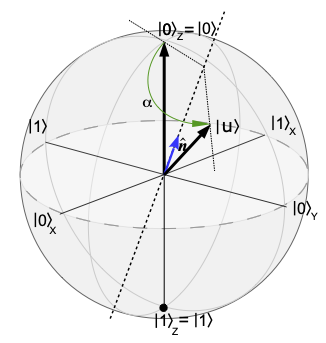
\includegraphics[width=0.3\linewidth]{Figuras/Fig_puertas_simples_BlochSphere_rot.png}
	\caption{Una rotación en la esfera de Bloch representada por un eje de rotación y el ángulo que se rota entorno al mismo. Figura tomada de \cite{Curso-JMas}}
	\label{Fig_puertas_simples_BlochSphere_rot.png}
	\end{figure}

En la Ec. (\ref{ec_puertas_simples_Rn}) el término $\hat{\bf n}\cdot \boldsymbol{\sigma}$ se refiere a la multiplicación de un vector por un vector de matrices. Esto es, multiplicar cada matriz por un elemento del vector y sumar las 3 matrices resultantes. Es decir, en la Ec. (\ref{ec_puertas_simples_Rn}) tenemos la suma de 4 matrices 2x2. La matriz resultante es
	
	\begin{equation} \label{ec_puertas_simples_Rn_matrix}
	R_{\hat{\bf n}}(\alpha)~  ~=~ \large{\lp \begin{matrix} 
	\cos \frac{\alpha}{2} - i n_z\sin\frac{\alpha}{2} 
	& (-in_x- n_y)\sin\frac{\alpha}{2} \\ 
	(-in_x + n_y) \sin\frac{\alpha}{2} 
	&  \cos \frac{\alpha}{2} + i n_z\sin\frac{\alpha}{2} 
	\end{matrix} \rp}
	\end{equation}
			

\Ejercicio{Calcular la matriz (\ref{ec_puertas_simples_Rn_matrix}) a partir de (\ref{ec_puertas_simples_Rn})}

        \subsection{Rotaciones en X, Y, Z}

Veamos los casos particulares de las rotaciones entorno a los ejes $x$, $y$ y $z$.        
\begin{align}
\bm \hat{n} = (0,0,1) \rqa R_z(\alpha) & = 
	 \lp \begin{matrix}
	 e^{-i \alpha/2} & 0                       \\
	 0               & e^{i \alpha/2} 
	 \end{matrix} \rp   \label{ec_puertas_simples_Rz} \\
\bm \hat{n} = (0,1,0) \rqa R_y(\alpha) & =
	 \lp \begin{matrix}
	 \cos \alpha/2     &  -\sin \alpha/2       \\
	 \sin \alpha/2     &  \cos \alpha/2 
	 \end{matrix} \rp  \label{ec_puertas_simples_Ry} \\
\bm \hat{n} = (1,0,0) \rqa R_x(\alpha) & = 
	 \lp \begin{matrix}
	 \cos \alpha/2       &   -i \sin \alpha     \\
	 -i \sin \alpha/2    &   \cos \alpha/2 
	 \end{matrix} \rp \label{ec_puertas_simples_Rx}
\end{align} 
        
        \subsection{Parametrización de Euler} \label{sec_subsub_puertas_euler}
        
Hay otra parametrización para las rotaciones mucho más común en física y es la \textbf{parametrización de Euler}. A diferencia de la anterior, esta no necesita definir ningún eje extra usando un vector, sino que simplemente consiste en tres rotaciones, con tres ángulos, entorno a dos ejes coordenados: primero entorno al eje $z$, después en torno al eje $y$ y finalmente entorno al eje $z$ otra vez\footnote{Podría usarse otro orden de ejes, como por ejemplo $xyx$ o $yzy$.}. Es decir
	\begin{equation} \label{ec_puertas_simples_rotacion_1}
	R_z(\phi) R_y (\theta) R_z(\varphi) = e^{- \frac{i}{2} (\phi + \varphi)} U (\theta, \phi, \varphi),
	\end{equation}
donde 
	
	\begin{equation} \label{ec_puertas_simples_rotacion_U}
	\boxed{U (\theta, \phi, \varphi) = \large{ \lp \begin{matrix}
	\cos \frac{\theta}{2}                &  - e^{i\varphi} \sin \frac{\theta}{2} \\
	e^{i \phi} \sin \frac{\theta}{2}     &  e^{i (\varphi + \phi)} \cos \frac{\theta}{2}
	\end{matrix} \rp}}
	\end{equation}

y donde $\theta$, $\phi$ y $\varphi$ se denominan \textbf{ángulos de Euler}. Véase que nuevamente podemos ignorar la fase global que nos sale en la Ec. (\ref{ec_puertas_simples_rotacion_1}) y quedarnos solo con la matriz $U (\theta, \phi, \varphi)$.

Podemos ver que la acción del operador (\ref{ec_puertas_simples_rotacion_U}) sobre el estado $\ket{0}$ nos da la expresión genérica del estado de un qúbit que vimos en la Ec. (\ref{ec_qubit_caso_general}):
	\begin{equation}
	U (\theta, \phi, \varphi) \ket{0} = 
	U (\theta, \phi, \varphi) \begin{bmatrix} 1 \\ 0 \end{bmatrix} = 
	 \cos{\frac{\theta}{2}}\, |0\rangle + e^{i\varphi}\sin{\frac{\theta}{2}}\,|1\rangle
	\end{equation}
También podemos ver que la acción del operador de este operador sobre la base computacional $\lch \ket{0}, \ket{1} \rch$ nos la una base alineada con el eje $(\theta, \phi)$:
	\begin{equation}
	U(\theta,\phi,\varphi) \ket{0} = 
		\large{\begin{bmatrix} \cos \frac{\theta}{2}  \\ e^{i\phi} \sin \frac{\theta}{2} \end{bmatrix} }
	~~~~~~,~~~~~~~
	U(\theta,\phi,\varphi) \ket{1} = 
		\large{\begin{bmatrix} -e^{i\varphi}\sin \frac{\theta}{2} \\ e^{i(\varphi + \phi)} \cos \frac{\theta}{2} \end{bmatrix} }
	\end{equation}

    \section{Puertas simples}

La computación clásica se basa en la descomposición de algoritmos complejos en una serie de puertas lógicas elementales. Veremos que lo mismo ocurre con la computación cuántica.  

Por puertas simples entendemos un conjunto de \textbf{operadores unitarios} que se utilizan con frecuencia en la computación cuántica. Vamos a ver las puertas simples sobre 1 qúbit. 

		\subsection{Dos formas de escribir las matrices 2x2.}   

Primero hagamos un breve alto en el camino para vez una segunda forma de escribir las matrices $2\times2$ en computación cuántica. Dada una matriz genérica $A$ podemos escribirla como
\begin{equation}
A = \lp \begin{matrix}
a_{11} & a_{12} \\
a_{21} & a_{22}
\end{matrix} \rp = 
a_{11} \ketbra{0}{0} + a_{12} \ketbra{0}{1} +  a_{21} \ketbra{1}{0} +  a_{22} \ketbra{1}{1} 
\end{equation}
Esta segunda forma es cómoda para hacer operaciones. 

	\begin{mybox_blue}{Nota: producto de interno de estado de la base}
	Como los elemtos de la base son ortonormales cumplen:
	\begin{equation}
	\braket{0}{0} = \braket{1}{1} = 1, ~~~~~~~~ \braket{0}{1}=\braket{1}{0}=0.
	\end{equation}
	Ahora podemos ver como antúa una matriz genérica $A$ sobre un elemento de la base, por ejemplo, $\ket{0}$
	\begin{align*}
	A \ket{0} & = a_{11} \ket{0}\braket{0}{0} + a_{12} \ket{0} \cancel{\braket{1}{0}} +  
		a_{21} \ket{1}\braket{0}{0} +  a_{22} \ket{1} \cancel{\braket{1}{0}} \\
	& = a_{11} \ket{0}\braket{0}{0} + a_{21} \ket{1}\braket{0}{0} = a_{11} \ket{0} + a_{21}\ket{1} =
	\begin{bmatrix} a_{11} \\ a_{21} \end{bmatrix}
	\end{align*}
	

	\end{mybox_blue}
	
        \subsection{Puertas de fase} 
		    \SubsubiIt{$P_\alpha$ con $\alpha \in [ 0, 2\pi ) $.}

Se trata de una rotación entorno al eje $Z$ y se escribe de la forma		    
	\begin{equation}
	\boxed{P(\alpha)= \lp \begin{matrix}
	1 & 0 \\ 0 & e^{i\alpha} 
	\end{matrix} \rp =  \ketbra{0}{0} + e^{i\alpha}\ketbra{1}{1}}
	\end{equation}
Aplicando sobre un estado genérico tenemos
	\begin{equation*}
	P(\alpha) \ket{u} =  
	\lp \begin{matrix} 1 & 0 \\ 0 & e^{i\alpha} \end{matrix} \rp 
	\begin{bmatrix} \cos\theta/2 \\ e^{i\phi}  \sin\theta/2 \end{bmatrix} =
	 \begin{bmatrix} \cos\theta/2 \\ e^{i(\phi+\alpha)}  \sin\theta/2 \end{bmatrix} = 
	 \ket{v}
	\end{equation*}

Ya vimos en la Ec. (\ref{ec_puertas_simples_Rz}) una puerta para rotar entorno al eje $z$. Podemos ver que a efectos prácticos la puerta $P_\alpha$ es lo mismo que la puerta $R_z(\alpha)$, pues se diferencian solo en una fase global
	\begin{equation*}
	P_\alpha \equiv e^{i \alpha/2} R_z (\alpha)
	\end{equation*}
		    
		    		    
		    \SubsubiIt{$K_\alpha$}  

Esta puerta es trivial pero a veces se usa en algunas demostraciones. Se trata simplemente de una puerta de fase global
	\begin{equation}
	K(\alpha)= e^{i\alpha} \lp \begin{matrix} 1 & 0 \\ 0 & 1 \end{matrix} \rp =  
	e^{i\alpha} \lp  \ketbra{0}{0} + \ketbra{1}{1} \right) = e^{i\alpha} I 
	\end{equation}
    	
        \subsection{Puertas discretas}
        
            \SubsubiIt{$X$, $Y$, $Z$}

Tres puertas muy usadas en computación cuántica con las siguientes
\begin{align}
&\boxed{X = \lp  \begin{matrix}0&1\\1&0\end{matrix} \rp = \sigma_x = \ketbra{1}{0} + \ketbra{0}{1}}~, ~~~  \label{ec_puertas_simples_X} \\ \rule{0mm}{7mm}
&\boxed{Y = \lp \begin{matrix}0&-i\\i&0\end{matrix} \rp = \sigma_y  =  i \ketbra{1}{0} - i \ketbra{0}{1}}~, ~~~ \label{ec_puertas_simples_Y}\\ \rule{0mm}{7mm}
&\boxed{Z = \lp  \begin{matrix}1&0\\0&-1\end{matrix} \rp = \sigma_z = \ketbra{0}{0} - \ketbra{1}{1}}  ~, ~~~ \label{ec_puertas_simples_Z}
\end{align}
donde hemos remarcado la igualdad con las \textit{matrices de Pauli} (ver sección \ref{sec_qubit_matrices_Pauli}).

\Ejercicio{Relacionar  $X,Y,Z$ con   $R_x(\alpha),R_y(\alpha)$ y $R_z(\alpha)$ par algún valor de $\alpha$.}
            
	\begin{mybox_blue}{Nota}
	Como las puertas $X$, $Y$ y $Z$ son las matrices de Pauli, estas son hermíticas ($A = A^\dagger$) y 
	además cumplen que son iguales a su inversa (ver Ec. (\ref{ec_qubit_pauli_sigma^2})). 
	Esto implica que aplicar dos veces seguidas una de estas puertas es lo mismo que aplicar la identidad. 
	Además, los autovalores de las matrices de Pauli son $\pm 1$ (ver Ecs. (\ref{ec_qubit_sigma_det}) y (\ref{ec_qubit_sigma_tr})).
	\end{mybox_blue}


            \SubsubiIt{$S$, $T$}

Cualquier potencia $U^k$ de un operador unitario es otro operador unitario. Esto es fácil de demostrar cuando $k=2$ pero es cierto en el caso general $k\in{\mathbb R}$. Así obtenemos

	\begin{equation}
	\boxed{S = Z^{1/2} =  \lp\begin{matrix}1&0\\0&i\end{matrix}\rp = \lp\begin{matrix}1&0\\0&e^{i\pi/2}\end{matrix} \rp}
	~~~~~,~~~~~~ 
	\boxed{T = S^{1/2} = \lp \begin{matrix} 1&0 \\ 0 & e^{i\pi/4} \end{matrix} \rp} \, .
	\end{equation}
            
            \SubsubiIt{$H$}
       
La puerta de Hadamard, $H$, es la primera puerta \textbf{genuinamente cuántica} en el sentido de que lleva un estado de la base a una superposición coherente

	\begin{equation}
	H \ket{0} = \frac{1}{\sqrt{2}}\left(\rule{0mm}{4mm}\ket{0} + \ket{1}\right) =\ket{+} 
	 ~~~~~~~~,~~~~~~~~~~
	H \ket{1} = \frac{1}{\sqrt{2}}\left(\rule{0mm}{4mm}\ket{0} - \ket{1}\right) =\ket{-} 
	\end{equation}

Podemos escribir este operador en la base $H = H_{ij}\ketbra{i}{j}$
	\begin{align*}
	H &=  \ket{+}\bra{0} +  \ket{-}\bra{1} \\
	  &= \frac{1}{\sqrt{2}}(\ketbra{0}{0} + \ketbra{1}{0} + \ketbra{0}{1} - \ketbra{1}{1})
	\end{align*}
de  lo que obtenemos la representación matricial
	\begin{equation} \label{ec_puertas_simples_H}
	\boxed{H   =  \frac{1}{\sqrt{2}} \lp \begin{matrix} 1 & 1 \\ 1 & -1 \end{matrix} \rp}
	\end{equation}

	\begin{mybox_blue}{Nota: otra expresión para la Hadamard}
	En cálculos posteriores encontraremos muy útil la siguiente representación de la acción de $H$
	\begin{equation} \label{ec_puertas_simples_H_sobre_1_qubit}
	\boxed{H \ket{x} =\frac{1}{\sqrt{2}} \sum_{y=0,1} (-1)^{ x  y} \ket{y}}
	\end{equation}
	\end{mybox_blue}

Como cualquier puerta, la acción de $H$ puede visualizarse como una rotación en la esfera de Bloch. En este caso una es una rotación de $\pi$ radianes en torno a un eje diagonal situado a 45$^\circ$ entre el eje $x$ y el eje $y$. Esta rotación permuta los ejes $x$ y $z$ y cambia de sentido el eje $y$.

\begin{equation}
\hat{\bf n} = \frac{1}{\sqrt{2}}(1,0,1) \rqa 
R_{\hat{\bf n}}(\pi) ~ = ~ -i\frac{1}{\sqrt{2}} \lp \begin{matrix} 1  & 1 \\ 1 & -1  \end{matrix} \rp =-i H \sim H 
\end{equation}

	\begin{mybox_blue}{Nota: La puerta de Hadammar es hermítica}
	Puede verse fácilmente que la puerta de Hadamard es hermítica e igual a su inversa. Es decir, aplicar
	dos veces seguidas la puerta de Hadamard es como aplicar la identidad.
	\end{mybox_blue}


        \subsection{Descomposición}
        
Una noción muy importante en computación cuántica es la descomposición de una puerta en producto de otras más simples. 

Para el caso de $H$, un poco de visión espacial muestra que su acción equivale a la composición de
\begin{itemize}
	\item una  rotación de $\pi/2$ radianes sobre el eje $y$ 
	\item seguida de una rotación de  $\pi$ radianes en torno al eje $x$.
\end{itemize}
Lo demostramos algebraicamente (despreciando fases globales)       
	\begin{align*}
	R_x(\pi)R_{y}\left(\frac{\pi}{2}\right) & = 
	\lp \begin{matrix}0&-i\\-i&0\end{matrix}  \rp
	\lp \begin{matrix}\cos\pi/4& -\sin\pi/4 \\ \sin\pi/4 & \cos\pi/4 \end{matrix} \rp = \\
	& = \frac{1}{\sqrt{2}} \lp \begin{matrix} 0&1 \\ 1&0 \end{matrix} \rp 
	\lp \begin{matrix}1 & -1 \\ 1 & 1 \end{matrix} \rp  =
	 \frac{-i}{\sqrt{2}} \begin{bmatrix}1&1\\1&-1\end{bmatrix} =-i H \sim H
	\end{align*}

	\Ejercicio{Encontrar los ángulos $\theta,\phi,\varphi$ que hay que verifican las siguientes idendidades
	 $$
	 U(\theta,\phi,\varphi) = H ~~~~,~~~~  U(\theta,\phi,\varphi) = SH
	 $$}

  
    \section{Circuitos Cuánticos (1 qubit)}
    
En un circuito cuántico un qubit se representa como una linea horizontal y las puertas que se aplican sobre 
el mismo se representan como cajas que contiene los datos del operador asociado. Por ejemplo, la aplicación del operador $U(\theta,\phi,\varphi)$ sobre un qubit en un estado $\ket{\psi}$, i.e.,
	\begin{equation*}
	\ket{\psi} \to  U(\theta,\phi,\varphi)\ket{\psi},
	\end{equation*}
se representa mediante el circuito siguiente
	\begin{figure}[H]
	\centering 
	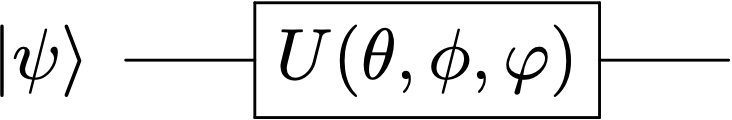
\includegraphics[width=0.3\linewidth]{Figuras/Fig_puertas_simples}
	\caption{Circuito para la operación $\ket{\psi} \to  U(\theta,\phi,\varphi)\ket{\psi}$. Figura tomada de \cite{Curso-JMas}}
	\label{Fig_puertas_simples}
	\end{figure}
	
 La concatenación de puertas se corresponde con la \textbf{composición de operadores}, es decir, con la \textbf{multiplicación de las matrices} asociadas. 

	\begin{mybox_blue}{Nota: Orden de las puertas}
	El \textbf{orden} en el que aparecen los operadores en la composición es el opuesto al que se 
	aprecia en el circuito. Así por ejemplo a la composición de operadores 
	$$
	\ket{\psi} \to  TH \ket{\psi} 
	$$
	le corresponde un circuito en el que  $H$ está a la izquierda de $T$. Recordemos que, por norma general,
	el producto de matrices no es conmutativo.
	\end{mybox_blue} 
 
 


		\subsection{Matriz de un circuito.}
		
Todo circuito se corresponde con un operador unitario que se obtiene componiendo todos los operadores que figuran en el. Por ejemplo, para el ejemplo $	\ket{\psi} \to  TH \ket{\psi}$, el circuito correspondiente representa el operador unitario $U$ al que le corresponde la matriz obtenida por multiplicación
	$$
	U = T H ~~~\to ~~~ U_{ij} = 
	\begin{bmatrix}1&0\\0&e^{i\pi/4}\end{bmatrix} \frac{1}{\sqrt{2}} 
	\begin{bmatrix} 1& 1 \\ 1 & -1 \end{bmatrix}  = 
	\frac{1}{\sqrt{2}} \begin{bmatrix} 1& 1 \\ e^{i\pi/4} & -e^{i\pi/4} \end{bmatrix} 
	$$

		\subsection{Simulador de un estado con qiskit.}
		
Veremos como construir y simular un estado con qiskit en la sección \ref{sec_medidas_subsub_codigo}, después de haber visto como medir.

















\chapter{Medidas, Parte I: Medida de 1 qúbit}

    \section{En la base computacional}
		\subsection{Superposiciones, medidas y colapso.}
	
En mecánica cuántica podemos tener un estado que sea la \textbf{superposición} de varios estado. Por ejemplo, el estado de un qúbit puede ser la superposición de los estados $\ket{0}$ y $\ket{1}$, esto es
%\begin{equation}
%\ket{\psi} = \alpha \ket{0} + \beta \ket{1} ~~, ~~~~ \text{con } |\alpha|^2 + |\beta|^2 = 1
%\end{equation}
	\begin{equation}
	\boxed{\ket{u} = \cos{\frac{\theta}{2}}\, |0\rangle + e^{i\varphi}\sin{\frac{\theta}{2}}\,|1\rangle }
	\end{equation}
Sin embargo, al medir solo obtenemos \textbf{uno de estos estado de la superposición}. La probabilidad de medir cada uno de estos estados que forman la superposición es igual 	\textbf{al módulo cuadrado del coeficiente que lo acompaña en el vector}  $\ket{\psi}$ (el módulo cuadrado de la amplitud de ese estado). En este caso vemos que la probabilidad de medir el estado $\ket{0}$ es $|\alpha|^2$ y la de medir $\ket{1}$ es $|\beta|^2$.


El aparato de medida estándar en computación cuántica asigna valores $\{0,1\}$ a los kets $\ket{0}$ y $\ket{1}$ de la base computacional. Su representación en un circuito podemos verla en la Fig. \ref{Fig_medidas1_cubit_meter}. En esta figura vemos que tenemos dos formas de medir: una destructiva y otra no destructiva. La explicación es simple: dependiendo de como esté construido el ordenador cuántico, nuestra medida destruirá o no el estado del qúbit al medirlo. 

En el caso en el que el estado no se destruya, lo que pasará será que el qúbit \textbf{colapsará} al estado medido. Esto es el famosos \textbf{colapso de la función de ondas} en mecánica cuántica. Si, por ejemplo, al medir nuestro qúbit obtenemos que estado $\ket{0}$, la superposición desaparece y nuestro qubit pasa a estar en el estado $\ket{0}$.

\begin{figure}[H] \setcounter{subfigure}{0} 
\centering
\subfigure[Medida no destructiva. \label{Fig_medidas1_cubit_meter1}]{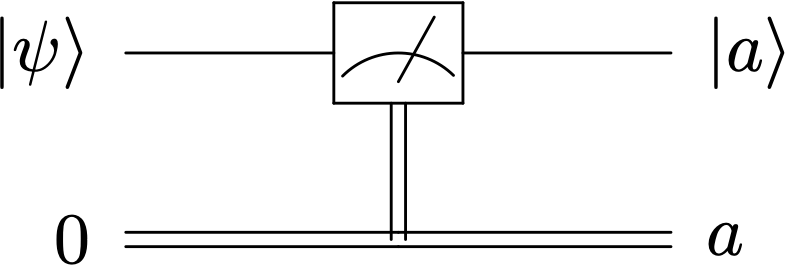
\includegraphics[width=0.3\linewidth]{Figuras/Fig_medidas1_cubit_meter1}}  \hspace{2cm}
\subfigure[Medida destructiva. \label{Fig_medidas1_cubit_meter2}]{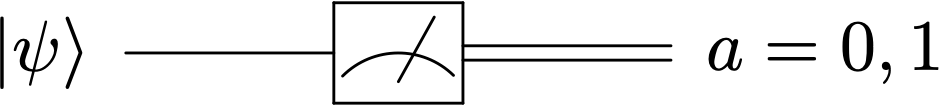
\includegraphics[width=0.3\linewidth]{Figuras/Fig_medidas1_cubit_meter2}} 
\caption{Medidas de un qubit en el estado $\ket{\psi}$ en un circuito cuántico. El resultado puede ser $a = 0$ o $a=1$. La linea simple representa un qubit, mientras que la linea doble representa un bit clásico. Figura tomada de \cite{Curso-JMas}}
\label{Fig_medidas1_cubit_meter}
\end{figure}

		\subsection{Sobre medir en la base computaciones.}

Los elementos de la base computacional $\ket{a}\in \{\ket{0},\ket{1}\}$, son autoestados del \textbf{observable} $Z = \sigma_z $, cuyos autovalores son $+1$ y $-1$ respectivamente, cumpliendo
$$
Z\ket{0} = +\ket{0}~~~~,~~~~~ Z\ket{1} = -\ket{1}
$$ 
Podemos unificar ambos resultados como: $Z\ket{a} = (-1)^a\ket{a}$, con  $a=\{0,1\}$. Es decir, lo que estamos haciendo es medir el observable $Z$ (por ejemplo, medir el espín en el eje $z$) y si obtenemos el autovalor $+1$ decimos que tenemos un 0, mientras que si medimos el autovalor $-1$, decimos que tenemos un $1$. 


		\subsection{Código de Qiskit: simulación de un estado y medida.}  \label{sec_medidas_subsub_codigo}

	\begin{mybox_orange}{Jypyter Notebook: 02-Circuitos\_1\_qubit\_medidas\_y\_RealHardware parte 1}
	En la primera parte del notebook \textbf{02-Circuitos\_1\_qubit\_medidas\_y\_RealHardware} puede verse como construir circuitos de un qúbit en qiskit, 
	como añadir puertas de un qúbit, como añadir los medidores y como hacer la simulación. Además de como guardar figuras de los
	circuitos y de como generar histogramas con los resultados.
	\end{mybox_orange}
	
		\subsection{Código de Qiskit: ejecución en un ordenador real.}
		
	\begin{mybox_orange}{Jypyter Notebook: 02-Circuitos\_1\_qubit\_medidas\_y\_RealHardware parte 2}
	En la segunda parte del notebook \textbf{02-Circuitos\_1\_qubit\_medidas\_y\_RealHardware} puede verse como mandar circuitos a ejecutar en ordenadores 
	cuánticos reales de IBM.
	\end{mybox_orange}
	
		

    \section{La moneda cuántica}
    
Vamos a ver aquí a modo de ejemplo un experimento simple: \textbf{la moneda cuántica.}

El resultado de tirar una moneda al aire es una variable aleatoria con dos resultados equiprobables:  cara y cruz.  Es irrelevante si analizamos el resultado cada tirada o cada dos, o tres tiradas. Las frecuencias relativas de caras y cruces, siempre serán próximas a $1/2$. Es decir, podemos tirar la moneda, recogerla sin mirarla, volver a tirar, y las probabilidades no cambian.

Podemos imaginar un experimento similar con un qúbit, donde cara $\to 0$ y cruz $\to 1$ son los resultados posibles de la medida en la base $Z$. Como al tirar la moneda, mientras esta está en el aire podemos pensar que está en ``una superposición equiprobable del cara y cruz'', el hecho de \textbf{tirar la moneda} en computación cuántica será aplicar el operador $H$ (ver Ec. (\ref{ec_puertas_simples_H})). 

Haciendo esta consideración, podemos ver que no es lo mismo tirar la moneda 1 vez y mirar 
$$
\ket{0}~ \stackrel{\rm tirar}{\longrightarrow} ~ H \ket{0}= \ket{+} ~ \stackrel{\rm medir}{\longrightarrow} ~p(0) = p(1) = 0.5
$$
que tirarla dos veces y mirar
$$
\ket{0}~ \stackrel{\rm tirar}{\longrightarrow} ~ H \ket{0}~ \stackrel{\rm tirar}{\longrightarrow} H^2\ket{0} = \ket{0} ~ \stackrel{\rm medir}{\longrightarrow} ~p(0) = 1 ~,~p(1) = 0
$$
El objetivo de este experimento es simplemente ver que ciertas puertas son sus propias inversas y que cuando aplicamos las aplicamos un número par de veces seguidas, es como si no aplicáramos nada. Otra cosa que podemos ver con este experimento es que \textbf{las medidas intermedias alteran el resultado}. Esto podemos verlo si colocamos un medidor en medio entre las puertas $H$ y vemos como varía el resultado.



		\subsection{Código de Qiskit.}
		
	\begin{mybox_orange}{Jypyter Notebook: 02-Circuitos\_1\_qubit\_medidas\_y\_RealHardware parte 3}
	En la tercera parte del notebook \textbf{02-Circuitos\_1\_qubit\_medidas\_y\_RealHardware} puede verse el experimento de la moneda cuántica.
	\end{mybox_orange}
    
    
    \section{Medidas en una base general}
        \subsection{Bases X, Y, Z} \label{sec_subsub_medidad1_bases_xyz}
       
A parte de la base computacional $\{\ket{0},\ket{1} \}$, es muy necesario y frecuente el uso de otras bases ortonormales como  $\{\ket{+},\ket{-} \}$ o  $\{\ket{+i},\ket{-i} \}$. Todas ellas diagonalizan algún operador de Pauli y, por  tanto, puede servir para construir aparatos de medida que discriminen entre sus estados       
\begin{align}
Z \ket{0} &=+ \ket{0}   , & Z \ket{1} &=-\ket{1} \\ 
X \ket{+} &=+ \ket{+}    ,& X \ket{-} &=-\ket{-} \\ 
Y \ket{+i} &=+ \ket{+i}  ,& Y \ket{-i} &=-\ket{-i}.
\end{align}    
En la práctica, solo solemos contar con un aparato de medida en la base computacional de autoestados de $\sigma_z$. La pregunta ahora es cómo podríamos utilizar  dicho aparato para efectuar medidas en las bases de autoestados de $\sigma_x$ y $\sigma_y$.

Por ejemplo desearíamos definir un aparato de medida que ``leyese'' los valores $0$ y $1$ para los autoestados $\ket{\pm}$ del opeador $\sigma_x =  X$ (ver Fig. \ref{Fig_medidas1_meter_xbasis2}).
	\begin{figure}[H]
	\centering 
	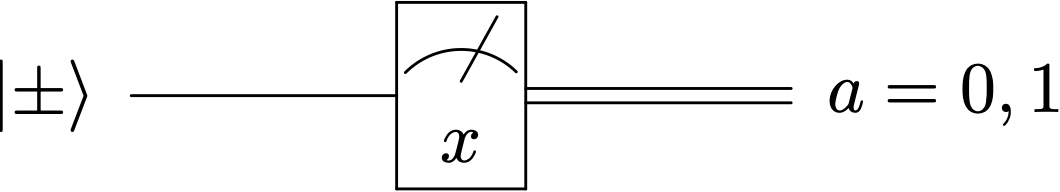
\includegraphics[width=0.3\linewidth]{Figuras/Fig_medidas1_meter_xbasis2}
	\caption{Medidor en la base $X$.}
	\label{Fig_medidas1_meter_xbasis2}
	\end{figure}
Análogamente, queremos los mismo para los autoestados $\ket{\pm i}$ de $\sigma_y = Y$. La clave está en un cambio de base (en rotar la base en la que queremos medir a la base $\lch \ket{0}, \ket{1} \rch$). 
\begin{align}
\ket{+}  &= H\ket{0}  ,&  \ket{-}  &= H\ket{1}    \\ 
\ket{+i}  &= SH \ket{0}    ,&  \ket{-i}  &= SH\ket{1}   .
\end{align}
Estas expresiones son facilmente invertibles para deshacer el cambio de base:
\begin{align}
H \ket{+}  &= \ket{0}                ,&  H\ket{-}  & = \ket{1}   \label{ec_medidas1_de_X_a_Z} \\ 
H S^\dagger \ket{+i}  &=  \ket{0}    ,&  H S^\dagger  \ket{-i}  & = \ket{1}   . \label{ec_medidas1_de_Y_a_Z}
\end{align}
Es decir, la idea es llevar a cabo una operación que nos lleve los elementos de la base en la que queremos medir (los elementos $\{\ket{+},\ket{-} \}$ o  $\{\ket{+i},\ket{-i} \}$) a los elementos de la base computacional $\{\ket{0},\ket{1} \}$. Esto es precisamente lo que conseguimos con los operadores $H$ y $H S^\dagger$ en las Ecs. (\ref{ec_medidas1_de_X_a_Z}) y (\ref{ec_medidas1_de_Y_a_Z}).
De las relaciones anteriores se deduce que
\begin{align}
X & = H Z H   \label{ec_medidas1_cambio_X-Z} \\
Y & = S  H  Z   H S^\dagger \label{ec_medidas1_cambio_Y-Z}
\end{align}

	\begin{mybox_blue}{Nota}
	Verifiquemos por ejemplo
	$$
	Y \ket{-i} = (SHZHS^\dagger )(SH\ket{0}) = SH Z\ket{1} =  SH(-\ket{1})= - SH\ket{1} = -\ket{-i}
	$$
	\end{mybox_blue}

	\Ejercicio{Comprueba estos cambios de base (las Ecs. (\ref{ec_medidas1_de_X_a_Z}), (\ref{ec_medidas1_de_Y_a_Z}), (\ref{ec_medidas1_cambio_X-Z}) y (\ref{ec_medidas1_cambio_Y-Z})).}
	
Estas relaciones nos permite definir el aparato de medida efectivo en las direcciones $x$ e $y$. Podemos verlos en la Fig. \ref{Fig_medidas1_meter_XYbasis}. 
    
	\begin{figure}[H]
	\centering 
	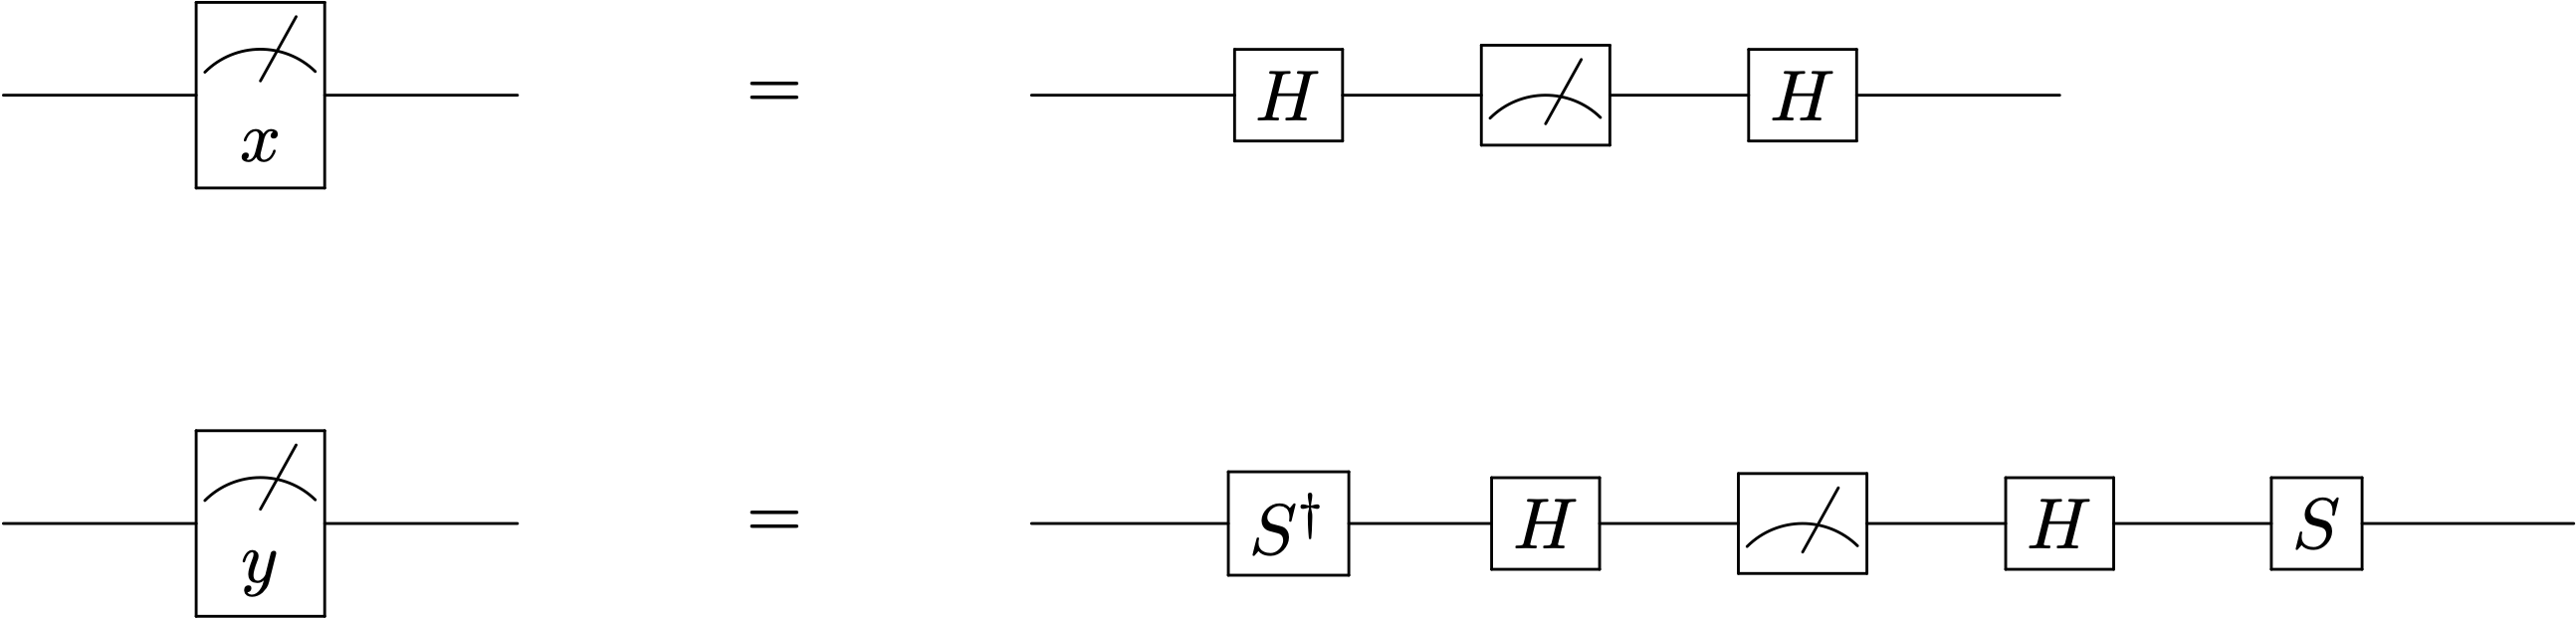
\includegraphics[width=0.8\linewidth]{Figuras/Fig_medidas1_meter_XYbasis}
	\caption{Equivalencias de los medidores en las bases $X$ e $Y$ con el medidor en $Z$. Cuando la medida es destructiva (la inmensa mayoría de las veces), no hace falta añadir los operadores después del aparato de medida.}
	\label{Fig_medidas1_meter_XYbasis}
	\end{figure}

     
        \subsection{Base arbitraria}

Vamos a generalizar el análisis anterior. Para ello podemos usar la matriz de rotación en la parametrización de Euler de la Ec. (\ref{ec_puertas_simples_rotacion_U}), que nos lleva la base base  $\lch \ket{0}, \ket{1} \rch_{\hat{\bm n}}$ asociado a un vector

\begin{equation}
\hat{\bm n} (\theta, \phi) = \sin \theta \cos \phi \hat{\bm x} + \sin \theta  \sin \phi \hat{\bm y} + \cos \theta \hat{\bm z}
\end{equation}

	\begin{figure}[H]
	\centering 
	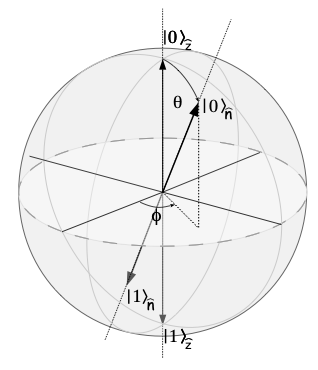
\includegraphics[width=0.3\linewidth]{Figuras/Fig_medidas1_BlochSphere_basis}
	\caption{Base computacional y base $\hat{\bm n}$ en la esfera de Bloch}
	\label{Fig_medidas1_BlochSphere_basis}
	\end{figure}

Es decir, tenemos el cambio de base
	\begin{equation}
	\ket{a}_{\hat{\bm n}} = U \lp \theta, \phi, 0 \rp \ket{a}_{\hat{\bm z}}, ~~~~ \text{con } a= 0,1 
	\end{equation}
que verifica la ecuación de autovalores
	\begin{equation}
	\sigma_z \ket{a}_{\hat{\bm z}} = (-1)^a \rqa (\hat{\bm n} \cdot \bm \sigma ) \ket{a}_{\hat{\bm n}} = (-1)^a \ket{a}_{\hat{\bm n}}
	\end{equation}
Por esta razón, podemos etiquetar este operado como
	\begin{equation}
	U(\theta,\phi,0) ~ \equiv ~ U(z\to \hat{\bf n})
	\end{equation}
para ver claramente que lo que hace es llevarnos de la base $Z$ a una base definida por $\hat{n}$.

El circuito de la Fig. \ref{Fig_medidas2_nbasis_measure2}  simula un aparato de medición en la base $\{\ket{a}_{\hat{\bf n}}\}_{a=0,1}$. Podemos ver que lo que se aplica antes del medidor en $Z$ no es $U(z\to \hat{\bf n})$ sino su inversa, $U(z\to \hat{\bf n})^\dagger$. Esto es porque lo que tenemos que hacer es llevar la base $\hat{\bm n}$ a la base $Z$.

	\begin{figure}[H]
	\centering 
	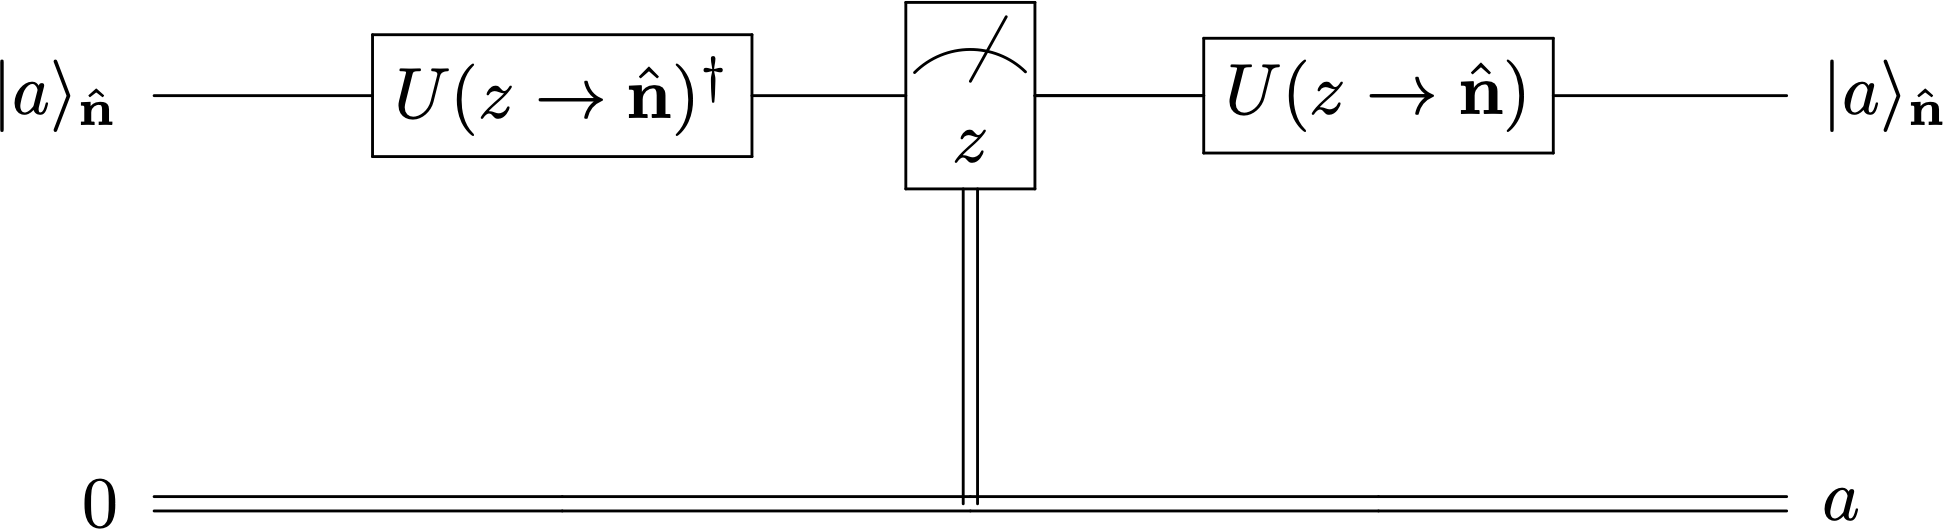
\includegraphics[width=0.7\linewidth]{Figuras/Fig_medidas2_nbasis_measure2}
	\caption{Medida en un eje arbitrario $\hat{ \bm n}$.}
	\label{Fig_medidas2_nbasis_measure2}
	\end{figure}

	\begin{mybox_blue}{Nota}
	Puede verse fácilmente que el caso genérico que acabamos de ver incluye, como es lógico
	los dos casos anterior:
	\begin{eqnarray}
 	U(\pi/2,0,\pi)=H : \ket{a}_{\hat{\bf z}} \to \ket{a}_{\hat{\bf x}} \\ \rule{0mm}{8mm}
 	U(\pi/2,\pi/2,\pi)= SH  : \ket{a}_{\hat{\bf z}} \to \ket{a}_{\hat{\bf y}}
	\end{eqnarray}
	\end{mybox_blue}
     
    


    \section{Valores esperados.}
    
    
Un estado es un objeto probabilístico que tiene una interpretación a través de los coeficientes (de las amplitudes de probabilidad) y por tanto, esa interpretación probabilística está ligada a una base. Es decir, las amplitudes de probabilidad no tiene sentido hasta que definimos una base en la que medir. Si por ejemplo, vamos a medir en la base $Z$, lo conveniente es expandir el estado en la base $Z$
$$
\ket{\psi} = c_0 \ket{0} + c_1 \ket{1}
$$
de forma que los coeficientes adquieren una interpretación probabilística. Puede decirse que las amplitudes ``no existen'' hasta que decidimos en que base medimos. El acceso experimental a estas amplitudes se da mediante estadística de las medidas
\begin{equation}
\boxed{p_0 = \frac{n_{0}}{N} = |c_0|^2 = |\braket{0}{\psi}|^2} ~~~~~~~~~~~~~~~~ \boxed{p_1 = \frac{n_{1}}{N}=|c_1|^2 =  |\braket{1}{\psi}|^2} \, .
\end{equation}
donde $N$ es el número total de medidas, $n_0$ es el número de medidas que arrojaron el valor 0 (en realidad +1) y $n_1$ es el número de medidas que arrojaron el valor 1 (en realidad -1).
Este procedimiento de reconstrucción es la base de la \textbf{tomografía cuántica}.



	    \subsection{Valor esperado de un observable arbitrario (operador hermítico). }
	    
Vamos a ver como se mide el valor esperado de un observable arbitrario $A$ en un estado arbitrario $\ket{\Psi}$. Estos valores esperados se denotan de la siguiente forma: $\langle Z \rangle_\Psi$. 

Cualquier observable sobre un cúbit cumple $A = A^\dagger$ (es hermítico) con lo que puede expresarse en la base
	\begin{equation} \label{ec_medidas1_expansion_A_en_Paulis}
	A = a I + n_x X + n_y Y  + n_z Z \, .
	\end{equation}
Los coeficientes se obtienen haciendo uso de las relaciones $\frac{1}{2}$ tr$ (\sigma_i \sigma_j) = \delta_{ij}$ y de tr$(\sigma_i)=0$, de las cuales se obtiene
	\begin{align}
	&\boxed{a  = \frac{1}{2} \text{ tr}(A)},        &         &\boxed{n_i = \frac{1}{2} \text{ tr}  (A \sigma_i)},
	\end{align} 
Entonces, podremos obtener el valor esperado de $A$  si somos capaces de medir los valores esperados de $X,$ $Y$ y $Z$.
	\begin{equation}
	\boxed{\langle A\rangle_\Psi = a + n_x \langle X\rangle_\Psi + n_y \langle Y\rangle_\Psi + n_z \langle Z\rangle_\Psi}
	\end{equation}

	 
			\SubsubiIt{$\langle Z \rangle_\Psi$} 
			
Los estados de la base computacional son autoestados del operador $Z$ con autovalor $\pm 1$
$$
Z \ket{0} =+ \ket{0}   ~~~~~~~~ ~~~~~~~~~~ Z \ket{1} =-\ket{1} 
$$
Dado un estado $\ket{\Psi} = c_0\ket{0} + c_1\ket{1}$, la medida repetida arroja de forma aleatoria los valores propios de $Z \to \pm 1$ con frecuencias relativas $n^Z_{0} $ y $n^Z_{1}$. Por definición, el valor esperado de dicha variable es, 
	\begin{equation} \label{ec_medidas1_valor_esperado_Z}
	\boxed{\langle Z \rangle_\Psi = (+1)\frac{n^Z_{0}}{N}+ (-1) \frac{ n^Z_{1}}{N}}
	\end{equation}
donde $N$ es el número total de medidas, $n_{0}^Z$ es el número de veces que hemos medido el estado $\ket{0}$ (el autovalor $+1$) y $n_{1}^Z$ es el número de veces que hemos medido el estado $\ket{1}$ (el autovalor $-1$).

Para medir $\langle Z\rangle_\psi$ necesitamos el \textbf{medidor habitual en computación cuántica} (ver Fig. \ref{Fig_medidas1_cubit_meter2})
			
			\SubsubiIt{$\langle X \rangle_\Psi$} 
			
Igualmente, si medimos el estado $\ket{\Psi}$ con un \textbf{medidor asociado al operador} $X = HZH$ (ver Fig. \ref{Fig_medidas1_meter_XYbasis}) la repetición arrojará igualmente una muestra aleatoria de valores propios de $X\to \pm 1$ con frecuencias relativas $n^X_0$ y $n^X_1$.
El valor esperado de $X$ se obtiene del promedio
	\begin{equation} \label{ec_medidas1_valor_esperado_Z}
	\boxed{\langle X \rangle_\Psi = (+1)\frac{n^X_{0}}{N}+ (-1) \frac{ n^X_{1}}{N}}
	\end{equation}
donde $N$ es el número total de medidas, $n_{0}^X$ es el número de veces que hemos medido el valor 0 (el estado $\ket{+}$ con autovalor $+1$ ) y $n_{1}^X$ es el número de veces que hemos medido 1 (el estado $\ket{-}$ con autovalor $-1$).
			
			\SubsubiIt{$\langle Y \rangle_\Psi$} 
			
Igualmente, si medimos el estado $\ket{\Psi}$ con un \textbf{medidor asociado al operador} $X = SHZHS^\dagger$ (ver Fig. \ref{Fig_medidas1_meter_XYbasis}) la repetición arrojará igualmente una muestra aleatoria de valores propios de $X\to \pm 1$ con frecuencias relativas $n^X_0$ y $n^X_1$.
El valor esperado de $X$ se obtiene del promedio
	\begin{equation} \label{ec_medidas1_valor_esperado_Z}
	\boxed{\langle Y \rangle_\Psi = (+1)\frac{n^Y_{0}}{N}+ (-1) \frac{ n^Y_{1}}{N}}
	\end{equation}
donde $N$ es el número total de medidas, $n_{0}^Y$ es el número de veces que hemos medido el valor 0 (el estado $\ket{+i}$ con autovalor $+1$ ) y $n_{1}^Y$ es el número de veces que hemos medido 1 (el estado $\ket{-i}$ con autovalor $-1$).		


	\Ejercicio{Genera un observable arbitrario hermítica $2\times 2$ $A$ y obten los coeficiente $n_i$ de la descomposición de $A$. 
	Inicializa un vector $\ket{\Psi}$ aleatorio y calcula el valor esperado $\langle A \rangle_\Psi$. (Todo a mano, con papel y bolígrafo)}
	


        \subsection{Valor esperado de un operador unitario (no necesariamente hermítico)}
        
En la sección anterior vimos como calcular el valor esperado de un operador hermítico aprovechando que los operadores de esta clase se pueden descomponer en función de las matrices de Pauli. Cuando el operador no es hermítico, no podemos llevar a cabo esta descomposición. Veamos como podemos calcular el valor esperado de un operador unitario genérico $V$.

En general, en computación cuántica partimos teniendo los qubit inicializados en el estado $\ket{0}$. Si queremos tener el estado $\ket{\Psi}$ debemos realizar una serie de operaciones sobre el qúbit para tenerlo. Estas operaciones pueden representarse por un operador  $U$ tal que $\ket{\Psi} = U\ket{0}$. 

Supongamos ahora que queremos calcular el valor esperado de un operador \textbf{unitario} $V$ en este estado $\ket{\Psi}$. Podemos calcularlo de la siguiente forma:
$$
\langle V \rangle_\Psi = \bra{\Psi}V\ket{\Psi} = \bra{0} U^\dagger V U\ket{0} = \braket{0}{\tilde \Psi}
$$

donde $\ket{\tilde\Psi} \equiv U^\dagger V U\ket{0}$ y la acción del operador unitario $U^\dagger V U$ (que no tiene porqué ser hermítico) se realiza mediante un circuito inicializado en $\ket{0}$.  Midiendo $\ket{\tilde \Psi}$  en la base $Z$, la fracción relativa de resultados $+1\to  n_0/N$ nos da acceso al \textbf{módulo del valor esperado}, 
$$
\sqrt{ \frac{n_{0}(\tilde\Psi)}{N} } ~=~  \sqrt{p_0}  ~=~   | \braket{0}{\tilde \Psi}|  ~=~ |\bra{\Psi}V\ket{\Psi}|    = |\langle V \rangle_\Psi |
$$
Podemos ver el circuito necesario para calcular este valor esperado en la Fig. \ref{Fig_medidad1_vev_unitary_V}.
	\begin{figure}[H]
	\centering 
	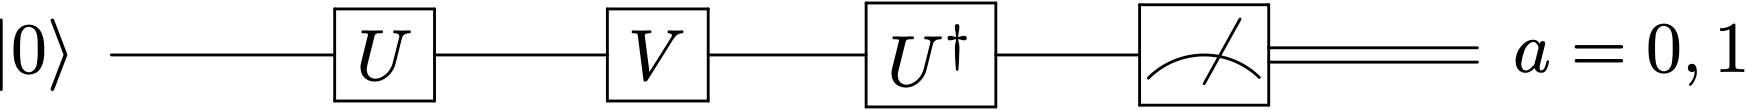
\includegraphics[width=0.6\linewidth]{Figuras/Fig_medidas1_vev_unitary_V.png}
	\caption{Circuito necesario para medir $\langle V\rangle_{\Psi} $ donde $\ket{\Psi} = U\ket{0}$ es un estado preparable.}
	\label{Fig_medidad1_vev_unitary_V}
	\end{figure}

	\begin{mybox_blue}{Nota: operadores unitarios y hermíticos}
	Si $V$ además de ser \textbf{unitario}, fuese \textbf{hermítico}, entonces tendríamos acceso al valor esperado completo, 
	al tratarse de una candidad real. 
	Operadores de 1 cúbit unitarios y hermíticos son, por ejemplo, los operadores $V = X,Y,Z,H$. 	
	Este argumento nos permite calcular de otra manera 	
	\begin{equation} \label{ec_medidas1_valores_esperados_XYZ}
	\left. 
	\begin{array}{c} \langle Z\rangle_\psi \\ \rule{0mm}{8mm} \langle X\rangle_\psi \\ \rule{0mm}{8mm} \langle Y\rangle_\psi \end{array}
	\right\} ~=~\braket{0}{\tilde\psi} ~=~ \sqrt{\frac{n_{0}(\tilde\psi)}{N}} ~~~\hbox{con}~~~~
	\left\{ 
	\begin{array}{l}  \ket{\tilde \psi} = U^\dagger  Z  U\ket{0} \\ \rule{0mm}{8mm} \ket{\tilde \psi} = U^\dagger H Z H U\ket{0}  \\ 
	\rule{0mm}{8mm}  \ket{\tilde \psi} = U^\dagger SH Z HS^\dagger U\ket{0} \end{array}
	\right.
	\end{equation}
	
	\end{mybox_blue}
	
	
	\begin{mybox_orange}{Jypyter Notebook: 02-Circuitos\_1\_qubit\_medidas\_y\_RealHardware parte 3}
	En la cuarta parte del notebook \textbf{02-Circuitos\_1\_qubit\_medidas\_y\_RealHardware} pueden verse cálculos de valores esperados con Qiskit.
	\end{mybox_orange}
    
		
		
		
		
		
		
		
		
		
		
		
		
		
		
		


\chapter{Multi-qubit: definiciones y puertas.}

Vamos ahora a empezar a ver que pasa cuando tenemos \textbf{más de un qúbit}. 

    \section{Algunas definiciones}
    
		\subsection{Estados multi-qubit.}

 Sea $\{ \ket{i}\}_{i=0,1}$ la base computacional del espacio de Hilbert de un qúbit $\mathcal{H} = {\mathbb C}^2$
 
	\Definicion{
	La \textbf{base computacional de} $ \mathcal{H}^{\otimes n}$ está formada por todas las cadenas de elementos posibles
	$$
	\boxed{\ket{i_{n-1}}\otimes \ket{i_{n-2}}\otimes ... \otimes \ket{i_0} ~\equiv ~\ket{i_{n-1} i_{n-2}...i_0}}~
	$$ 
	donde $~ i_{n-1},\dots,i_0=0,1$ y donde $\otimes$ representa el \textbf{producto tensorial} de espacio de Hilbert.
	}
	
La \textbf{dimensión}  dim($\mathcal{H}^{\otimes n}$) = $2^n$ coincide con el número de combinaciones distintas posibles: 	$2\times 2...\times 2 = 2^n$.    

	\begin{mybox_blue}{Producto de Krönecker}
	
	Cuando tenemos que un espacio de Hilbert es un \textbf{producto tensorial} de espacios Hilbert, para construir los
	elementos de la base y los operadores tenemos que usar el \textbf{producto de Krönecker}. 
	
	Sean $A$ y $B$ dos operadores definidos respectivamente sobre $\mathcal{H}_1$ y $\mathcal{H}_2$. El operador 
	$C=A \otimes B$ actua sobre $\mathcal{H} = \mathcal{H}_1 \otimes \mathcal{H}_2$ de la forma siguiente
	\begin{equation} \label{ec_multiqubit_C=AxB_1}
	C \ket{v} = A \otimes B \equiv \ket{Av_1} \otimes \ket{Bv_2} = \ket{\omega_1} \otimes \ket{\omega_2} \equiv \ket{\omega}
	\end{equation}
	y linealmente sobre sumas de vectores de $V$. 
	
	Para el caso en que $A$ y $B$ son de dimension $2\times 2$, el producto de Kronecker se puede escribir como
	\begin{equation}
	A \otimes B = \lp \begin{matrix}
	a_{11} B & a_{12} B \\
	a_{21} B & a_{22} B
	\end{matrix}	 \rp = 
	\lp \begin{matrix}
	a_{11} b_{11} & a_{11} b_{12} & a_{12} b_{11} & a_{12}b_{12} \\
	a_{11} b_{21} & a_{11} b_{22} & a_{12} b_{21} & a_{12}b_{22} \\
	a_{21} b_{11} & a_{21} b_{12} & a_{22} b_{11} & a_{22}b_{12} \\
	a_{21} b_{21} & a_{21} b_{22} & a_{22} b_{21} & a_{22}b_{22} 
	\end{matrix} \rp
	\end{equation}
	Para el caso de dos matrices columna (como son los vectores de la base):
	\begin{equation}	
	\begin{bmatrix} a_1 \\ a_2 \end{bmatrix} \otimes \begin{bmatrix} b_1 \\ b_2 \end{bmatrix} = 
	\begin{bmatrix} a_1 b_1 \\ a_1 b_2 \\ a_2 b_1 \\ a_2 b_2	\end{bmatrix}
	\end{equation}
	Puede verse más información en, por ejemplo, \cite{wiki_kronecker}.
	\end{mybox_blue}

El multi-ínidice $i_{n-1}i_{n-2}....i_0$ interpretarse como un número entero escrito en base \textbf{binaria}
	\begin{equation} \label{ec_multiqubit_notacion_binaria}
	\boxed{i_n i_{n-1}...i_1 ~~\longleftrightarrow ~~~p = \sum_{k=1}^n 2^{k-1} i_k}
	\end{equation}
que tomará  $2^n$ valores $p = 0,1,...,2^{n}-1$. El cambio de notación 
$$
\textit{multi-índice} ~ \leftrightarrow ~ \textit{entero en notación decimal} 
$$
será frecuente y se aplicará a cualquier elemento. Por ejemplo $\ket{000} = \ket{0}, \ket{111} = \ket{7}$ etc.	
	

	\begin{mybox_green}{Ejemplo 2-qúbits}
	Por ejemplo, para un sistema de 2-qúbits,   $n=2$ y tendríamos $2^n=2^2 = 4$ y entonces
	$$
\ket{00}~=~ \ket{0}\otimes \ket{0}~=~
\begin{bmatrix}1\\ 0\end{bmatrix}\begin{bmatrix}1\\ 0\end{bmatrix} = \begin{bmatrix}1\\0\\0 \\ 0\end{bmatrix}
~~~~~~,~~~~~
\ket{01}~=~ \ket{0}\otimes \ket{1}~=~
\begin{bmatrix}1\\ 0\end{bmatrix}\begin{bmatrix}0\\ 1\end{bmatrix} = \begin{bmatrix}0\\1\\0 \\ 0\end{bmatrix}
$$
$$
\ket{10}~=~ \ket{1}\otimes \ket{0}~=~
 \begin{bmatrix}0\\ 1\end{bmatrix}\begin{bmatrix}1\\ 0\end{bmatrix} = \begin{bmatrix}0\\0\\1 \\ 0\end{bmatrix}
 ~~~~~,~~~~
\ket{11}~=~ \ket{1}\otimes \ket{1}~=~
\begin{bmatrix}0\\ 1\end{bmatrix}\begin{bmatrix}0\\ 1\end{bmatrix} = \begin{bmatrix}0\\0\\0 \\ 1\end{bmatrix}
$$
	Las etiquetas de los vectores y, por tanto, de las componentes de las matrices, bi-índices $ij=11,12,21,22$ 
	que adopta el mismo número, $N^2$, de cofiguraciones distintas. 
	\end{mybox_green}


El vector de estado más general  $\ket{u}\in \mathcal{H}^{\otimes n}$ será una combinación lineal de elementos de la base computacional $\ket{i_n i_{n-1}...i_1}$ en términos de unas componentes $u_{i_ni_{n-1}...i_1}$
	\begin{equation} \label{ec_multiqubit_u_general}
	\boxed{\ket{u} = \sum_{i_0,i_1,..,i_{n-1}=0,1} u_{i_{n-1}ni_{n-2}...i_0} \ket{i_{n-1} i_{n-2}...i_0}  = \sum_{k=0}^{2^n-1} u_k \ket{k}},
	\end{equation}
donde hemos usado alternativamente la notación binaria y la decimal. 

	\begin{mybox_green}{Ejemplo}
	Para $n=2$ tendremos, en notación binaria  

	\begin{equation*}
		\begin{array}{ccc}
	\ket{u} ~&=& ~ \sum_{i,j=0,1} u_{ij} \ket{ij}~=~ u_{00}\ket{00}+ u_{01}\ket{01} + u_{10}\ket{10} +u_{11}\ket{11}
	\\ \\
	~&=&~ u_{00}\begin{bmatrix}1\\0\\0 \\ 0\end{bmatrix}+ u_{01}  \begin{bmatrix}0\\1\\0 \\ 0\end{bmatrix} + u_{10}
	\begin{bmatrix}0\\0\\1\\0\end{bmatrix}+u_{11}  \begin{bmatrix}0\\0\\0\\1\end{bmatrix}   ~ = 
	\begin{bmatrix}u_{00}\\ u_{01}\\ u_{10} \\ u_{11}  \end{bmatrix}
	\end{array}
	\end{equation*}

	y en notación decimal, para el mismo vector
	\begin{equation*}
	\begin{array}{ccc}
	\ket{u} ~&=& ~ \sum_{k=0}^{2^2-1=3} u_{k} \ket{k}~=~ u_{0}\ket{0}+ u_{1}\ket{1} + u_{2}\ket{2} +u_{3}\ket{3}
	\\ \\
	~&=&~ u_{0}\begin{bmatrix}1\\0\\0 \\ 0\end{bmatrix}+ u_{1}  \begin{bmatrix}0\\1\\0 \\ 0\end{bmatrix} + u_{2} 
	\begin{bmatrix}0\\0\\1\\0\end{bmatrix}+u_{3}  \begin{bmatrix}0\\0\\0\\1\end{bmatrix}   ~ = 
	\begin{bmatrix}u_{0}\\ u_{1}\\ u_{2} \\ u_{3}  \end{bmatrix}
	\end{array}
	\end{equation*}

	No debería haber confusión entre ambas notaciones puesto que, en cuanto aparezca un número superior a 1 quiere decir que 
	estamos tratando con la base decimal. 
	\end{mybox_green}

	\Ejercicio{Escribe el vector $\ket{u} = (1+i)\ket{101} -2\ket{010} + 3\ket{111}$ normalizado}
   

   
    \section{Entrelazamiento}



De forma  general, los estados $\ket{u}\in \mathcal{H}^{\otimes n}$ pertenecen a dos conjuntos disjuntos
\begin{itemize}
	\item Estados \textbf{factorizables}, cuando $\ket{u} = \ket{a}\otimes \ket{b}\otimes...\otimes \ket{c}$
	\item Estados \textbf{entrelazados}, cuando $\ket{u}$ no es factorizable
\end{itemize}

Ejemplos de estados factorizables serían
\begin{align*}
\ket{ \Psi} & = \frac{1}{\sqrt{4}} \lp \ket{00} + \ket{01} + \ket{10} + \ket{11} \rp = 
\frac{1}{\sqrt{4}} \lp \ket{0} + \ket{1} \rp \otimes \lp \ket{0} + \ket{1} \rp \\
\ket{ \Psi} & = \frac{1}{\sqrt{2}} \lp  \ket{10} + \ket{11} \rp = 
\frac{1}{\sqrt{4}}  \ket{1}  \otimes \lp \ket{0} + \ket{1} \rp \\
\end{align*}
Veremos un poco más sobre el entrelazamiento en la sección \ref{sec_subsub_multiqubit_medidas_parciales}






    	\subsection{Base de Bell}

Hasta ahora las bases que hemos usado eran todas de elementos factorizables. Podemos sin embargo usar también bases cuyo elementos sean vectores entrelazados. El ejemplo más común de base entrelazada es la \textbf{base del Bell}:
\begin{itemize}
	\item \textbf{Base computacional (factorizable)}: $\{ \ket{00},\ket{01},\ket{10},\ket{11} \}$
	\item \textbf{Base de Bell (entrelazada)}: 
	\begin{equation} \label{ec_multiqubit_Bell_states}
	\begin{array}{rcl}
	\ket{B_{00}} &=& \frac{1}{\sqrt{2}} \big( \ket{00} + \ket{11} \big) \vspace{3mm} \\ 
	\ket{B_{01}} &=& \frac{1}{\sqrt{2}} \big( \ket{01} + \ket{10} \big) \vspace{3mm} \\ 
	\ket{B_{10}} &=& \frac{1}{\sqrt{2}} \big( \ket{00} - \ket{11} \big) \vspace{3mm} \\ 
	\ket{B_{11}} &=& \frac{1}{\sqrt{2}} \big( \ket{01} - \ket{10} \big) \\
	\end{array}
	\end{equation}
\end{itemize}

        \subsection{Medidas parciales} \label{sec_subsub_multiqubit_medidas_parciales}

Una medida parcial afecta sólamente a un subconjunto de qúbits de un multi-qúbit. Es decir, solo afecta a uno o varios de los espacios de Hilbert, pero no a todos. Aquí encontramos una diferencia crucial entre estados factorizados y entrelazados. 		
		
			\SubsubiIt{Medidas parciales en un estado factorizable.}
			 


Consideremos el estado bi-qúbit \textbf{factorizable} 
$$
\ket{u} = \ket{a}\otimes \ket{b} = \frac{1}{\sqrt{2}}\big( \ket{0} + \ket{1}\big)\otimes \frac{1}{\sqrt{2}}\big( \ket{0} + \ket{1}\big)\, .
$$
Una medida sobre el primer qúbit solo podrá resultar, con probabilidad $1/2$, en uno de los dos posibles estados siguientes  
$$
\ket{u} ~\rightarrow ~ \left\{ \begin{matrix}\ket{0} \otimes \frac{1}{\sqrt{2}}\big( \ket{0} + \ket{1}\big)\\ \ket{1} \otimes \frac{1}{\sqrt{2}}\big( \ket{0} + \ket{1}\big) \end{matrix} \right.
$$
Vemos que, después de esta medición, el segundo qúbit permanece intacto. Es decir, si medimos el segundo qúbit seguimos teniendo una probabilidad 1/2 de medir $\ket{0}$ o $\ket{1}$.

			\SubsubiIt{Medidas parciales en un estado factorizable.}

Sin embargo, si el estado es \textbf{entrelazado}, por ejemplo, 
$$
  \ket{B_{00}} = \frac{1}{\sqrt{2}}\big( \ket{00} + \ket{11} \big)\, ,
$$
una medida sobre el primer cúbit hace colapsar el segundo a uno de los dos siguientes posibles estados
$$
\ket{B_{00}} ~\rightarrow ~ \left\{ \begin{matrix}\ket{0}\otimes\ket{0}  \\ \ket{1}\otimes \ket{1}\end{matrix} \right. \, .
$$
también con probabilidad 1/2. Vemos que ahora, \textit{el segundo qúbit ha sufrido modificación  \textbf{correlacionada} con el resultado obtenido de la medida del primero qúbit}.  Es decir, una medida parcial sobre uno de los espacios de Hilbert está afrectando al otro espacio de Hilbert. 

	\begin{mybox_blue}{Entrelazamiento: acción fantasmal a distancia}
	Cuando se descubrió el entrelazamiento y las consecuencias que tenía sobre los estados al hecho de medir, a este efecto se lo denominó
	\textit{acción fantasmal a distancia}, y fue muy criticado por personalidades de la talla de Albert Einstein. 
	
	\vspace{0.3cm}
	Quizás con la explicación anterior no se entiende bien lo sorprendente del entrelazamiento y porque se lo denominó como acción fantasmal a distancia.
	Cuando hablamos de que tenemos \textit{dos espación de Hilbert} diferente, a lo que esto se (puede) traducir en la vida real es a que tenemos \textit{dos partículas}.
	Lo que hemos visto es que sí nuestro par de partículas está en un estado entrelazado \textit{medir el estado de una partícula afecta el estado de la otra}. 
	Esto es, cuanto menos, sorprendente. 

	\vspace{0.3cm}	
	Uno de los argumentos que usaban los detractores de la física cuántica para criticarla era precisamente el entrelazamiendo. El argumento es simple: si tenemos un par de 
	partículas en un estado entrelazado, nada nos impide separarlas y llevar cada una a una esquina del universo. Como están entrelazadas, si medimos una de ellas, 
	inmediatamente el estado de la otra partícula se ve afectado y también colapsa. Es decir, parece que hay una interacción que es capaz de hacer un efecto instantáneo 
	independientemente de la distancia que separe las partículas, lo cual viola un principio fundamental de la Relatividad Especial: \textit{nada puede viajar más rápido que 
	la velocidad de la luz en el vacío, ni siquiera las interacciones}. 

	\vspace{0.3cm}	
	Esta contradicción con la Relatividad se solventa teniendo en cuenta que \textit{no existe ninguna forma de usar partículas entrelazadas para transmitir información más 
	rápido que la velocidad de la luz}. Esto es simple de entender. Cuando tú tienes una de estas partículas entrelazadas no tienes forma de saber si la persona que tiene la 
	otra partícula ha decido medirla o no. En caso de que la otra persona midiera, la única forma de que tú sepas que ha medido es que te mande un mensaje y te lo diga. 
	Como este mensaje no puede viajar más rápido que la velocidad de la luz, no se viola la causalidad. 
	\end{mybox_blue}

\begin{itemize}
	\item En ambos casos,  las probabilidades de medir $\ket{0}$ ó $\ket{1}$ en el segundo cúbit, son idénticamente iguales a $1/2$.
	
	\item Eso implica que: mediciones sobre el segundo qúbit, \textit{no permiten desvelar} si el estado original era entrelazado o no. Es decir, si tienes repetido cientos de ves el mismo par de qúbits y decides solo medir un qúbit en cada par, no tienes forma de saber que está pasando en el otro qúbit del par, si ha colapsado al medir o no.
	
	\item Sin embargo, el entrelazamiento introduce un tipo de correlaciones muy sutiles que se pueden detectar haciendo medidas más sofisticadas, como las que conducen a las desigualdades de Bell. 
\end{itemize}


	\begin{mybox_blue}{Nota: Dos electrones entrelados}
	Una forma intuitiva de pensar en el entrelazamiento es pensar que dos partículas están entrelazadas cuando las medidas de sus estados están correlacionadas. El ejemplo clásico es del espín de dos electrones. Dos electrones pueden entrelazarse de forma que si mides que uno de ellos tiene espín $+1/2$, el otro tiene espín $-1/2$. 

	\vspace{0.3cm}
La gracia de este entrelazamiento es que ambos electrones están en un estado de superposición, de forma que el estado global del sistema es
$$
\ket{\Psi} = \ket{\uparrow \downarrow} + \ket{\downarrow\uparrow}
$$
Vemos que es una supersición, pero donde solo son posibles los estados en los que los electrones tienen estados al contrarios. Se ve fácilmente que este estado no es factorizable, con lo que es entrelazado. 
	\end{mybox_blue}



    \section{Circuitos Multiqubit}

Sea $\ket{a_{n-1}a_{n-2}...a_1a_0}$ un estado multiqúbit de la base computacional $a_{i} = 0,1$. Este estado se propaga a lo largo de un circuito de forma que \textit{cada línea representa un espacio de Hilbert}. 

La asignación que se hace en \textbf{Qiskit }coloca el qúbit \textbf{menos relevante }$a_0$  en la  línea superior. Esta ordenación en un circuito es la inversa de la que tradicionalmente se utiliza en la literatura (siguiendo la influencia del libro de Nielsen Chuang \cite{nielsen_chuang_2010}). Podemos ver esto en la Fig. \ref{Fig_multiqubits_convenios_ordenacion}

	\begin{figure}[H]
	\centering 
	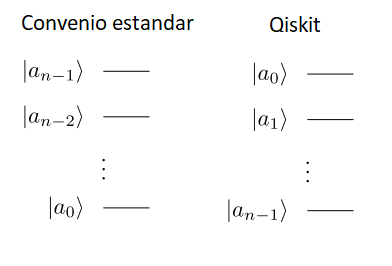
\includegraphics[width=0.4\linewidth]{Figuras/Fig_multiqubits_convenios_ordenacion}
	\caption{Convenios de ordenación de los qúbits en la forma estándar, resaltando que Qiskit decide usar el convenio al revés.}
	\label{Fig_multiqubits_convenios_ordenacion}
	\end{figure}


    \section{Puertas (multi-qubit) no controladas}

Vamos a ahora las puertas multi-qúbit más famosas.
   

        \subsection{Walsh-Hadamard}
        
El operador de Walsh-Hadammard es el producto tensorial de operadores de Hadammard
$$
W = H^{\otimes n} = H\otimes H \ldots \otimes H 
$$
La  acción  de $H^{\otimes n}$ sobre el estado de referencia $\ket{00...0}$ produce una \textbf{superposición uniforme} de todos los estados de la base.
	\begin{align*}
	W \ket{00...0} &= H\ket{0}\otimes H\ket{0} \otimes ... \otimes H\ket{0} \\  \rule{0mm}{8mm}
	& = \frac{1}{\sqrt{2}}\big(\ket{0}+\ket{1}\big)\otimes \frac{1}{\sqrt{2}}\big(\ket{0}+\ket{1}\big)\otimes ...\otimes \frac{1}{\sqrt{2}}\big(\ket{0}+\ket{1}\big)\\ \rule{0mm}{8mm}
	&= \frac{1}{2^{n/2}}\big(\ket{00...00} + \ket{00...01}+....+\ket{11...11} \big)
	\end{align*}



Vemos que esta puerta es factorizable. Podemos ver en la segunda línea de la ecuación anterior que, efectivamente, al partir de un estado factorizable seguimos teniendo un estado factorizable después de aplicar la Walsh-Hadammard. 

Es muy común que al principio de un circuito cuántico se aplique una Walsh-Hadammad a la mayoría de qúbits para generar la superposición uniforme (recordemos que en computación cuántica ser parte teniendo todos los qúbits en el estado $\ket{0}$, es decir, del estado $\ket{0\dots00}$).

Para ver la acción de de $H^\otimes$ sobre un estado multiqúbit es necesario recordar la Ec. (\ref{ec_puertas_simples_H_sobre_1_qubit}) (la acción de $H$ sobre un qúbit). Tenemos pues
	\begin{align*}
	H^{\otimes n} \ket{x} & = H\ket{x_{n-1}}\otimes H\ket{x_{n-2}}\otimes \ldots \otimes H\ket{x_0} \\  \rule{0mm}{5mm} 
	& = \sum_{y_{n-1}= \, 0,1} (-1)^{y_{n-1}x_{n-1}}\ket{y_{n-1}}\otimes \sum_{y_{n-2}=0,1} (-1)^{y_{n-2}x_{n-2}}\ket{y_{n-2}} \otimes \ldots \otimes  \sum_{y_{0}\, =\, 0,1} (-1)^{y_{0}x_{0}}\ket{y_{0}} \\  \rule{0mm}{5mm} 
	& = \sum_{y_{n-1}, y_{n-2},\ldots, y_{0}=\, 0,1} (-1)^{x_{n-1} y_{n-1}+ \ldots + x_0 y_0} \ket{y_{n-1}\ldots y_0}
	\end{align*}
es decir, 
	\begin{equation} \label{ec_multiqubit_Walsh_H_sobre_x}
	\boxed{H^{\otimes n} \ket{x} = \frac{1}{\sqrt{2^n}} \sum_{y \, =\, 0}^{2^n-1}(-1)^{x\cdot y} \ket{y}} ~~ \text{ donde } \boxed{x\cdot y = x_{n-1} y_{n-1} \oplus x_{n-1} y_{n-1} \oplus \ldots \oplus x_0 y_0}.
	\end{equation} 
Para el caso particular en que lo aplicamos sobre el estado $\ket{0\ldots00}$, tenemos
	\begin{equation} \label{ec_multiqubit_Walsh_H_sobre_0}
	\boxed{|\Psi_0 \rangle = H^{\otimes n} |0 \rangle^{n} = \frac{1}{\sqrt{N}}  \sum_{i=0}^{N=2^n} | i \rangle}.
	\end{equation}
Si nos fijamos, estamos haciendo $n$ operaciones y con ello estamos inicializando $2^n$ estados. Esta acción exponencialmente rápida es consecuencia de la superposición. No confundir superposión y entrelazamiento, son cosas diferentes. Aquí \textit{no tenemos entrelazamiento}.
        
        \subsection{SWAP}

La puerta SWAP es una puerta binaria fundamental (no factorizable), cuya acción consiste en permutar los estados existentes en los registros individuales sobre los que actúa. En particular, sobre los elementos de la base
	\begin{equation}
	\boxed{U_{\rm SWAP }: \ket{00}\to\ket{00}~~,~~\ket{01}\to\ket{10}~~,~~\ket{10}\to\ket{01}~~,~~ 	\ket{11}\to\ket{11} }
	\end{equation}
Esto nos permite escribir el operador en la notación de producto exterior y posteriormente como matriz
	\begin{equation}
	U_{\rm SWAP } = \ket{00}\bra{00} + \ket{01}\bra{10} + \ket{10}\bra{01} +\ket{11}\bra{11}  \rqa	
	U_{\rm SWAP} = \lp \begin{matrix} 1 & 0 & 0 & 0 \\ 0 & 0 & 1 & 0 \\ 0 & 1 & 0 & 0 \\ 0 & 0 & 0 & 1 \end{matrix} \rp
	\end{equation}
Podemos ver la representación gráfica asociada al operador SWAP en la Fíg. \ref{Fig_multiqubit_SWAP_gate}.

	\begin{figure}[H]
	\centering 
	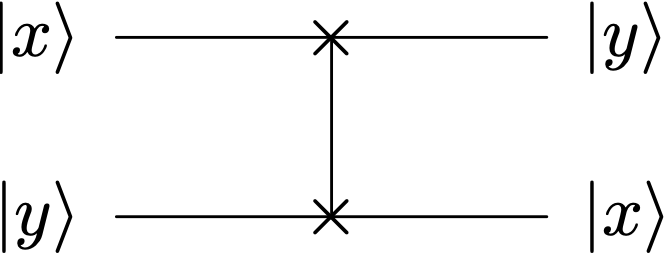
\includegraphics[width=0.23\linewidth]{Figuras/Fig_multiqubit_SWAP_gate}
	\caption{Puerta SWAP}
	\label{Fig_multiqubit_SWAP_gate}
	\end{figure}

    \section{Puertas controladas}
    
En las puertas controladas, un operador se aplica sobre un qúbit dependiendo del estado en el que se encuentra otro. Este segundo qúbit se denomina \textbf{controlador}, mientras que el primero es el \textbf{controlado}. Las puertas controladas son eficientes para generar entrelazamiento.
La puerta controlada  se representa como sigue
	\begin{equation}
	\boxed{\cg{U} = \ket{0}\bra{0}\otimes I + \ket{1}\bra{1}\otimes U}
	\end{equation}
donde $U$ es un operador unitario de 1-qúbit general. Si por el primer qúbit (el controlador)
\begin{itemize}
	\item entra $\ket{0}$, sale $\ket{0}$ y en el segundo cúbit (controlado) no se hace nada (se aplica $I$).
	\item entra $\ket{1}$, sale $\ket{1}$ y en el segundo cúbit (controlado) se aplica el operador $U$.
\end{itemize}
La \textbf{representación matricial} de $CU$ es fácil de obtener como suma de  \textbf{productos de Kronecker}
	\begin{equation}
	\cg{U} = \begin{bmatrix}1 & 0 \\ 0 & 0 \end{bmatrix}\otimes  I +  \begin{bmatrix}0 & 0 \\ 0 & 1 \end{bmatrix} \otimes U
= \begin{bmatrix} 1\times I & 0 \\ 0 & 0 \end{bmatrix}  + 
\begin{bmatrix} 0 & 0 \\ 0 & 1\times U \end{bmatrix} = \begin{bmatrix}   I & 0 \\ 0 &   U \end{bmatrix} = 
\begin{bmatrix} 1 & 0 & 0 & 0 \\ 0 & 1 & 0 & 0 \\ 0 & 0 & U_{11} & U_{12} \\
0 & 0 & U_{21} & U_{22}\end{bmatrix}
	\end{equation}

	\begin{mybox_blue}{Nota: Las puertas controladas son unitarias}
	Escrito de esta manera es evidente que, si $U$ es una matriz unitaria, $\cg{U}$ también lo es 
	$~\Rightarrow (\cg{U})^\dagger \cg{U} = I$. Esto no es algo trivial ya que la combinación lineal de operadores 
	unitarios, en general, no es  unitaria.
	\end{mybox_blue}

La acción de $\cg{U}$ sobre elementos de la base $\{\ket{x}\}$ donde $x=0,1$ admite una forma compacta 
	\begin{equation}
	\boxed{\cg{U}:\ket{x}\otimes\ket{y}  \rightarrow \ket{x} \otimes U^x\ket{y}}
	\end{equation}
Podemos ver la representación gráfica asociada al operador $\cg{U}$ en la Fíg. \ref{Fig_multiqubit_cU_gate}

	\begin{figure}[H]
	\centering 
	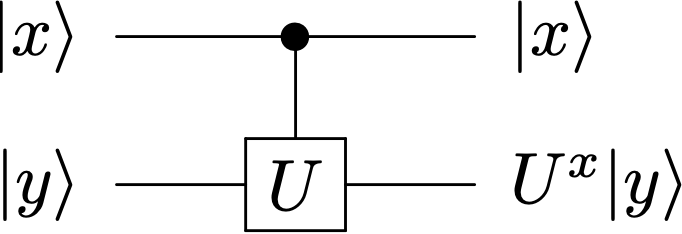
\includegraphics[width=0.25\linewidth]{Figuras/Fig_multiqubit_cU_gate}
	\caption{Puerta controlada}
	\label{Fig_multiqubit_cU_gate}
	\end{figure}
	
	\Ejercicio{Escribe un operador controlado y las matrices asociadas cuando  \begin{itemize}
		\item el qúbit de control es el segundo sobre el primero.
		\item el operador $U$ se aplica sobre el segundo cúbit, si el estado del primero es $\ket{0}$. \end{itemize}}



Operadores como éste existen en circuitos clásicos. La fascinante novedad es que, ahora, por el primer qúbit podría circular una superposición $a\ket{0} + b\ket{1}$. En estos casos, se efectuarían virtualmente las dos operaciones. El resultado de una acción controlada también conduce a una superposición, de forma tal que \textbf{se genera entrelazamiento}. 

Para verlo, hagamos actuar $\cg{U}$ sobre un estado de la forma  $\ket{\phi} = (a\ket{0} + b\ket{1})\otimes \ket{v}$, que es \textbf{factorizable}
	\begin{align*}
	\cg{U}\,\Lc (a\ket{0} +b \ket{1})\otimes \ket{v} \Rc
	& = \left(\ket{0}\bra{0}\otimes I + \ket{1}\bra{1}\otimes U\rule{0mm}{4mm}\right) \Lc (a\ket{0} +b \ket{1})\otimes \ket{v} \Rc \\ \rule{0mm}{5mm} 
    & = a\ket{0}\otimes \ket{v} + b\ket{1}\otimes U\ket{v}
	\end{align*}
Vemos que, efectivamente, el resultado es un estado entrelazado. Podemos ver esto en la Fig. \ref{Fig_multiqúbit_entangling_CU_circuit}.

	\begin{figure}[H]
	\centering 
	\includegraphics[width=0.5\linewidth]{Figuras/Fig_multiqúbit_entangling_CU_circuit}
	\caption{Entrelazamiento a partir de una puerta controlada.}
	\label{Fig_multiqúbit_entangling_CU_circuit}
	\end{figure}


        \subsection{CNOT} 
	
El caso más frecuente de una puerta binaria controlada es la puerta CNOT = $\cg{X}$
	\begin{equation} \label{ec_multiqubit_CNOT}
	\boxed{\hbox{CNOT} = \cg{X} ~=~ \ket{0}\bra{0}\otimes I + \ket{1}\bra{1}\otimes X }
	~=~ \begin{bmatrix} 1 & 0 & 0 & 0 \\ 0 & 1 & 0 & 0 \\ 0 & 0 & 0 & 1 \\ 0 & 0 & 1 & 0\end{bmatrix}
	\end{equation}
Sobre elementos de la base computacional $\ket{xy}=\ket{x}\otimes\ket{y}$ donde $\, x,y= 0,1$, su acción  se puede representar de manera compacta usando la suma módulo dos 
	\begin{equation} \label{ec_multiqubit_CNOT_compu}
	\boxed{\cg{X}:\ket{x}\otimes\ket{y} \rightarrow \ket{x} \otimes X^x\ket{y} = \ket{x} \otimes \ket{y\oplus x}}
	\end{equation}
Podemos ver la representación gráfica asociada al operador CNOT en la Fíg. \ref{Fig_multiqubit_cX_gate}
	\begin{figure}[H]
	\centering 
	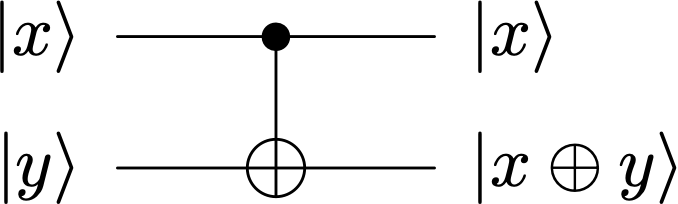
\includegraphics[width=0.25\linewidth]{Figuras/Fig_multiqubit_cX_gate}
	\caption{Puerta CNOT, CX o control-X}
	\label{Fig_multiqubit_cX_gate}
	\end{figure}

	\Ejercicio{El estado factorizable más general de dos cúbits es ($a$ es la normalización)
	$$
	\ket{\psi} = a \left(\ket{0} + b_1 e^{i\phi_1}\ket{1} \rp \lp \ket{0} + b_0 e^{i\phi_0} \ket{1} \right) 
	$$
	Escribe la condición más general que deben satisfacer  $b_0,b_1,\phi_0$ y $\phi_1$ para que CNOT$\ket{\psi}$ 
	sea un vector entrelazado. Nota: aplicar que para que un estado sea entrelazado el determinante de los coefientes es cero.}

	\begin{mybox_blue}{Nota: CNOT en Qiskit}
	La puerta CNOT en qiskit aparece invertida con respecto a la que dibujamos en la Fig. \ref{Fig_multiqubit_cX_gate}. Ello se debe a que qiskit ordena 
	los qubits en $\ket{q_1 \, q_0}$ poniendo el asociado al bit menos relevante $q_0$ arriba. 
	
	\vspace{0.3cm}
	Cuando en un circuito en Qiskit aparece una puerta como la de ls Fig. \ref{Fig_multiqubit_cX_gate} (con el control en el qúbit de arriba y aplicándose sobre el de abajo), como Qískit pone arriba el 
	bit menos significativos en realidad lo que tenemos en \textit{una CNOT donde el qúbit de control es el segundo}, es decir
		\begin{equation}
		\hbox{CNOT} = \cg{X} ~=~ I \otimes \ket{0}\bra{0} + X \otimes \ket{1}\bra{1} 
		~=~ \begin{bmatrix} 1 & 0 & 0 & 0 \\ 0 & 0 & 0 & 1 \\ 0 & 0 & 1 & 0 \\ 0 & 1 & 0 & 0\end{bmatrix}
		\end{equation}
	\end{mybox_blue}
	
	\begin{mybox_orange}{Jypyter Notebook: 03-Circuitos\_multiqubit secciones 1.1 y 1.2}
	En las secciones 1.1 y 1.2 del notebook \textbf{03-Circuitos\_multiqubit} pueden verse ejemplos de CNOTs y como crear entrelazamiento con ellas.
	\end{mybox_orange}
    

        \subsection{Control-SWAP}

Si el qúbit  de control está en  el estado $\ket{1}$ los dos controlados se intercambian. 
	\begin{equation} \label{Fig_multiqubit_CSWAP_gate}
	\boxed{U_{\rm CSWAP} =\ket{0}\bra{0} \otimes I_4 + \ket{1}\bra{1} \otimes U_{\rm SWAP}} \, .
	\end{equation}
Podemos verla en la Fig. \ref{Fig_multiqubit_CSWAP_gate}. 
	\begin{figure}[H]
	\centering 
	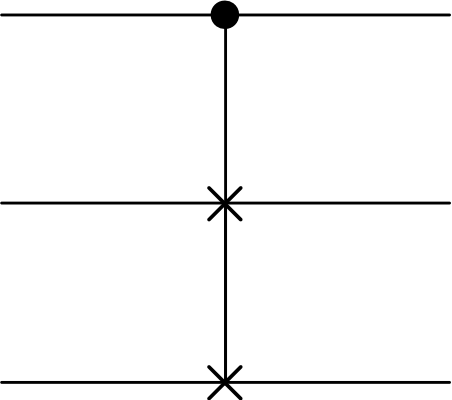
\includegraphics[width=0.13\linewidth]{Figuras/Fig_multiqubit_CSWAP_gate}
	\caption{Puerta CSWAP}
	\label{Fig_multiqubit_CSWAP_gate}
	\end{figure}

	\begin{mybox_orange}{Jypyter Notebook: 03-Circuitos\_multiqubit secciones 1.3 y 1.4}
	En las secciones 1.3 y 1.4 del notebook \textbf{03-Circuitos\_multiqubit} pueden verse ejemplos de SWAPs y CSWAPs
	\end{mybox_orange}

    \section{Puertas multicontroladas}
		\subsection{CCNOT o Toffoli}
		
La puerta CCNOT, también llamada puerta de Toffoli,  es un operador sobre $\mathcal{H}^{\otimes 3}$, en el que dos qúbits controlan la acción de $X$ sobre un tercero. \textbf{Sólo si ambos cúbits} de control están en el estado $\ket{11}$ el operador $X$ actuará sobre el tercero. De nuevo, su representación es muy sencilla
	\begin{equation}
	\boxed{{\rm CCNOT} = \big(\ket{00}\bra{00}+\ket{01}\bra{01}+\ket{10}\bra{10}\big)\otimes I + \ket{11}\bra{11}\otimes X}
	\end{equation}
Podemos ver la representación gráfica asociada la puerta de Toffoli en la Fíg. \ref{Fig_multiqubit_ccX_gate}
	\begin{figure}[H]
	\centering 
	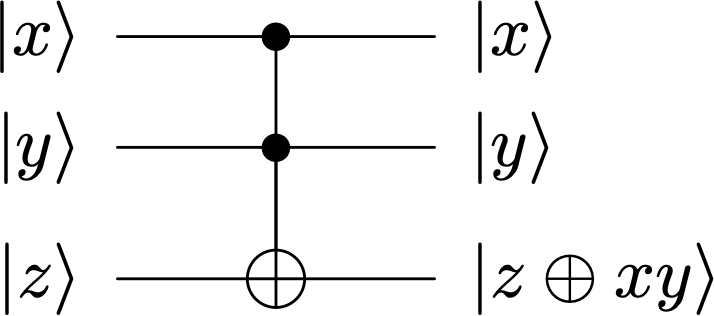
\includegraphics[width=0.22\linewidth]{Figuras/Fig_multiqubit_ccX_gate}
	\caption{Puerta de Toffoli o CCX.}
	\label{Fig_multiqubit_ccX_gate}
	\end{figure}
	
	\begin{mybox_orange}{Jypyter Notebook: 03-Circuitos\_multiqubit secciones 1.5}
	En las sección 1.5 del notebook \textbf{03-Circuitos\_multiqubit} pueden verse ejemplos de puertas Toffoli.
	\end{mybox_orange}

	\Ejercicio{a) Obtener la matriz que representa la puerta de Toffoli en la base computacional. Reproducirla usando Qiskit. b) Obtener la matriz de un circuito de 3 cúbits con una puerta CNOT en la que el tercer cúbit controla el primero. Reproducirla usando qiskit.}
	
		\subsection{$X$ multi-controlada.}
		
Cuando tenemos una puerta $X$ con tres o más controles, la denominamos $X$ multi-controlada (\textbf{MCX)}. La puerta $X$ se activa sí y solo sí los qúbits de control están en una configuración deseada. Podemos ver un ejemplo de MCX que se activa con el estado $\ket{1100}$ en la Fig. \ref{Fig_multiqubit_MCX_gate}  . El operado asociado esta puerta sería
$$
MCX = \ket{1100}  \bra{1100}\otimes X + (I-\ket{1100}\bra{1100}) \otimes I
$$

	\begin{figure}[H]
	\centering 
	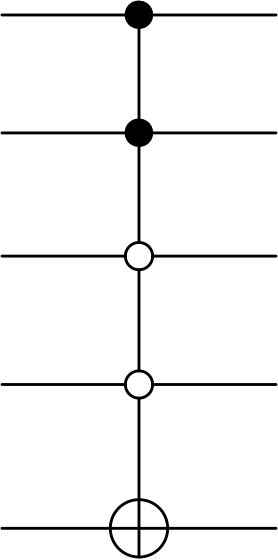
\includegraphics[width=0.1\linewidth]{Figuras/Fig_multiqubit_MCX_gate}
	\caption{Puerta MCX (multi-controled X) para el estado de control $\bra{1100}$. Recordemos que con Qiskit sería el revés.}
	\label{Fig_multiqubit_MCX_gate}
	\end{figure}

	\begin{mybox_blue}{Nota: controles con $\ket{0}$}
	Los botones blancos denotan controladores que se activan si el cúbit es $\ket{0}$. Esencialmente son iguales 
	a un controlador negro con una puerta $X$ antes y otra después.
	\end{mybox_blue}

	\begin{mybox_orange}{Jypyter Notebook: 03-Circuitos\_multiqubit secciones 1.6}
	En las sección 1.6 del notebook \textbf{03-Circuitos\_multiqubit} pueden verse ejemplos de puertas MCX.
	\end{mybox_orange}

    



















\chapter{Medidas, Parte II: Medida de estados multi-Qubit}

	\section{Medidas en la base computacional}

Un aparato de medida en la base asociada al operador hermítico $\sigma_z^{\otimes n} = Z\otimes \ldots \otimes Z$ hace colapsar el estado  que mide a un elemento $\ket{x}$ de la \textbf{base computacional}, que identificamos mediante una cadena de bits $a_{n-1}...a_0$ con $a_i=0,1$,  donde $x= a_{n-1}2^{n-1}+...+2^0 a_0$. Podemos ver esto en la Fig. \ref{Fig_medidas2_Multimeter_zbasis}

	\begin{figure}[H]
	\centering 
	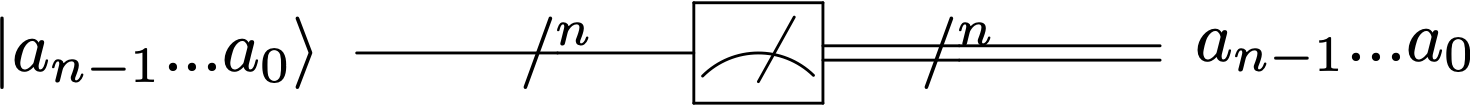
\includegraphics[width=0.5\linewidth]{Figuras/Fig_medidas2_Multimeter_zbasis}
	\caption{Medidor en la base $Z$. En este caso, midiendo destructivamente. Podría no ser el caso.}
	\label{Fig_medidas2_Multimeter_zbasis}
	\end{figure}




    \section{Medidas en bases generales}
    
Vamos a suponer que queremos medir en una base ortonormal arbitraria $\{\ket{ x}'\}$, $x=0,...,2^n-1$. Buscamos un circuito que, a la llegada de un vector  concreto de la base $\ket{x}'=\ket{a_{n-1}...a_0}'$, devuelva exactamente \textbf{la misma colección} de bits  $a_{n-1}...a_0$. Para ello, al igual que vimos en el caso de un qúbit, debemos conocer el operador $U$ que relaciona esta base con la base computacional
$$
\ket{ x}'= U\ket{x}~~~~~~\Longrightarrow ~~~~~~   U^\dagger\ket{x}' = \ket{ x}  \, .
$$
Entonces es evidente que sólo tenemos que añadir el operador $U^\dagger$ antes de usar el medidor estándar. Podemos ver esto en la Fig. \ref{Fig_medidas2_Multimeter_basis}. 

	\begin{figure}[H]
	\centering 
	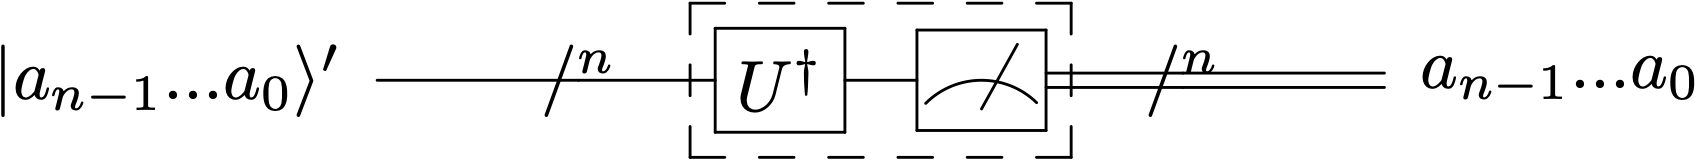
\includegraphics[width=0.6\linewidth]{Figuras/Fig_medidas2_Multimeter_basis}
	\caption{Medidor en una base arbitraria.}
	\label{Fig_medidas2_Multimeter_basis}
	\end{figure}


 
        \subsection{Medidas de Pauli}

En caso más frecuente consiste en medir diferentes qúbits en diferentes bases de Pauli, $X$, $Y$ ó $Z$. En este caso, $U= R_1\otimes \ldots \otimes R_n$ es un producto de rotaciones locales. Esto sigue la misma pauta que se explicó para el caso de un sólo qúbit (ver sección \ref{sec_subsub_medidad1_bases_xyz}). Podemos ver un ejemplo en la Fig. \ref{Fig_medidas2_XYZ_multimeter}.

	\begin{figure}[H]
	\centering 
	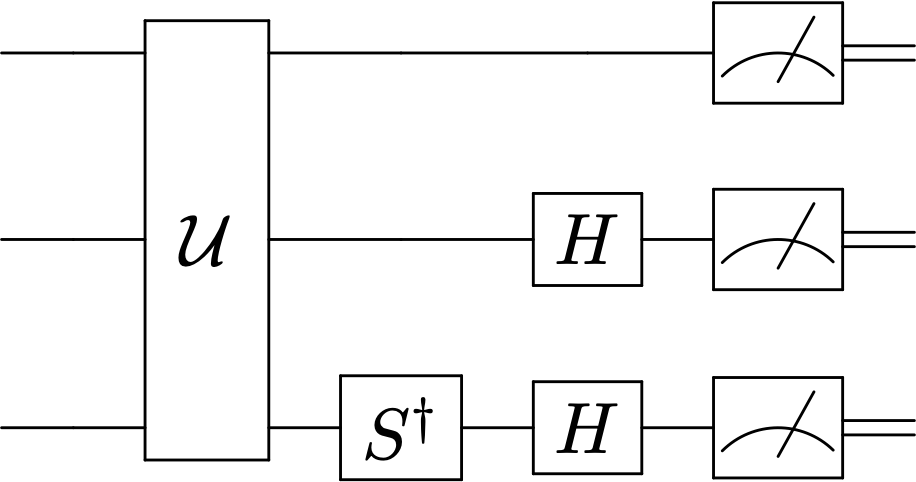
\includegraphics[width=0.3\linewidth]{Figuras/Fig_medidas2_XYZ_multimeter}
	\caption{Ejemplo de un circuito que mide en la base $Z_0X_1Y_2$ (el qúbit de arriba se mide en la base $Z$, el de en medio e la base $X$ y el de abajo en la base $Y$).}
	\label{Fig_medidas2_XYZ_multimeter}
	\end{figure}


	\begin{mybox_orange}{Jypyter Notebook: 04-Medidas\_II  seccion 1}
	Ver la sección 1 del notebook \textbf{04-Medidas\_II}.
	\end{mybox_orange}


        \subsection{Medidas de Bell}

Podemos medir también en bases entrelazadas, por ejemplo, en la base de Bell. En la Ec. (\ref{ec_multiqubit_Bell_states}) podemos ver la base de Bell 
	\begin{equation} \label{ec_medidas2_base_Bell_from_Z}
	\ket{B_{xy}} = \ket{xy}'  = U \ket{xy}.
	\end{equation}
En esta última expresión, $\ket{xy}$ está expresado en la base computacional.  El circuito que genera esta base puede verse en la Fig. \ref{Fig_medidas2_circuit_Bell_basis}. Sabemos que el circuito de medida debe de llevar antes de los medidores el inverso de este circuito. Podemos ver el circuito de medida en la base de Bell en la Fig. \ref{Fig_medidas2_Bell_meter}.

	\begin{figure}[H]
	\centering 
	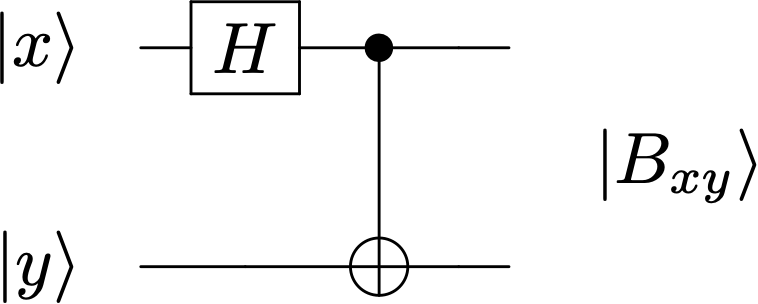
\includegraphics[width=0.25\linewidth]{Figuras/Fig_medidas2_circuit_Bell_basis}
	\caption{Circuito que genera la base de Bell a partir de la base computacional (ver Ec. (\ref{ec_medidas2_base_Bell_from_Z}).}
	\label{Fig_medidas2_circuit_Bell_basis}
	\end{figure}

	\begin{figure}[H]
	\centering 
	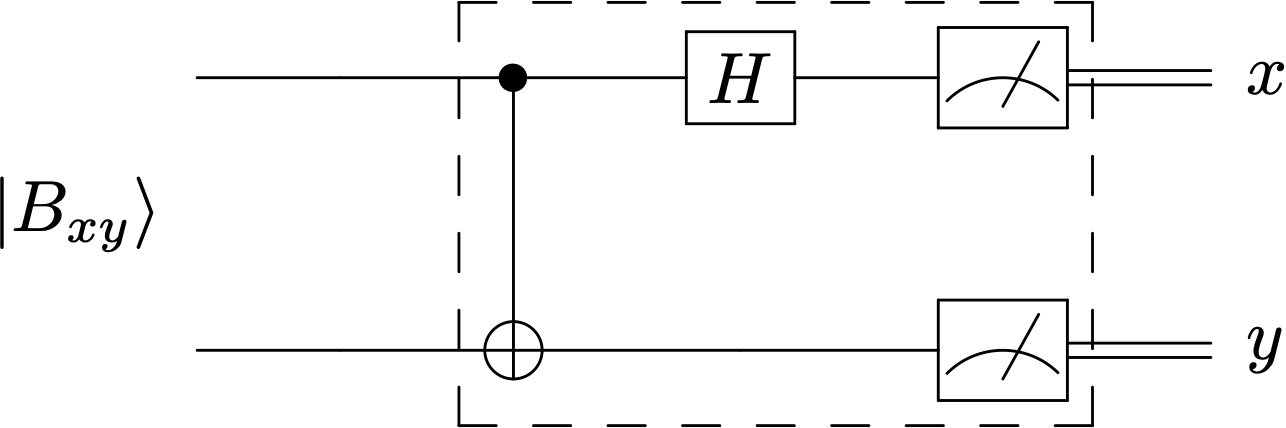
\includegraphics[width=0.4\linewidth]{Figuras/Fig_medidas2_Bell_meter}
	\caption{Medidor en la base de Bell. }
	\label{Fig_medidas2_Bell_meter}
	\end{figure}

	\begin{mybox_orange}{Jypyter Notebook: 04-Medidas\_II seccion 2}
	Ver la sección 2 del notebook \textbf{04-Medidas\_II}.
	\end{mybox_orange}


    \section{Valores esperados}

Como ya vimos en el caso de un qúbit, para calcular el valor esperado de un observable $A\in {\rm L}(H^{\otimes n})$ debemos expandirlo en una base de \textbf{cadenas de Pauli}
	\begin{equation} \label{ec_medidas2_A_en_cadenas_de_Pauli}
	A = \sum_{i_1,...,i_n=0}^3 a_{i_1\ldots i_n} \sigma_{i_1}\otimes \ldots \otimes \sigma_{i_n}
	\end{equation}
donde $\sigma_i = (I,X,Y,Z)$. Los coeficientes se pueden obtener haciendo las trazas
	\begin{equation} \label{ec_medidas2_coef_A_en_cadenas_de_Pauli}
	a_{i_1\ldots i_n} =\frac{1}{2^n} \text{tr } (A \,  \sigma_{i_1}\otimes \ldots  \otimes\sigma_{i_n})
	\end{equation}

Por lo tanto, para hallar el valor esperado de un operador $A$, solo tenemos que hallar los valores esperados de las cadenas de Pauli
	\begin{equation}
	\langle A \rangle_{\psi} =  \sum_{i_1,...,i_n=0}^3 a_{i_1\ldots i_n} \langle \sigma_{i_1}\otimes \ldots   \otimes\sigma_{i_n}\rangle
	\end{equation}

	\begin{mybox_orange}{Jypyter Notebook: 04-Medidas\_II seccion 3}
	Ver la sección 3 del notebook \textbf{04-Medidas\_II}.
	\end{mybox_orange}

	\Ejercicio{Calcula el valor esperado de $\langle X\otimes Y\otimes Z\rangle_\Psi$, donde 
	$$
	\ket{\psi} = \frac{i}{4} \ket{000}+\frac{1}{\sqrt{8}} \ket{001}+\frac{1+i}{4} \ket{010}+
	\frac{1+2i}{\sqrt{8}}\ket{101}+\frac{1}{4} \ket{110}
	$$   }
	
	\Ejercicio{Considera el hamiltoniano $H=A(X X+Y Y+Z Z)$ siendo $A=1.47\cdot 10^{-6}eV$. Calcular el 
	valor esperado de la energía $E = \langle H\rangle_\Psi$  en los cuatro estados de Bell 
	$\ket{\Psi} = \ket{B_{ij}}$. }



    \section{Medida de Hadamard}
    
    	\subsection{Valor esperado de un operador a partir de $\langle X \rangle$ y $\langle Y\rangle$}

Al final, el valor esperado de un operador es un simple número que se obtiene a partir de una distribución aleatoria de valores. 
¿No podríamos diseñar una variable aleatoria cuyo valor medio coincida con ese resultado? 
La medida de Hadamard hace precisamente esto aprovechando el entrelazamiento.


	\Teorema{
	Sea el circuito de la Fig. \ref{Fig_medidas2_Hadamard_measure}, donde por uno de los qúbits (el qúbit ancilla) entra el estado $\ket{+}$, por el otro entra el estado $\ket{\psi}$, se aplica el operador $U$ sobre qúbit en el estado $\ket{\psi}$ controlado por el qúbit en el estado $\ket{+}$ y se mide este último qúbit. Esta medida se hace bien usando un medidor en la base $X$ (ver Fig. \ref{Fig_medidas2_Hadamard_measurea}) o un medidor en la base base $Y$ (ver Fig. \ref{Fig_medidas2_Hadamard_measureb}). Calculando los valores esperados de $\langle X \rangle $ e $\langle Y \rangle$ en este qúbit ancilla (en la base computacional)
	\begin{equation}
	\langle X \rangle_{ancilla} = (+1) \frac{n^x_0}{n_0^x+n_1^x} + (-1) \frac{n^x_1}{n^x_0+n^x_1} ~~~~, ~~~~
	\langle Y \rangle_{ancilla} = (+1) \frac{n^y_0}{n^y_0+n^y_1} + (-1) \frac{n^y_1}{n^y_0+n^y_1}
	\end{equation}	
podemos calcular el valor esperado del operador $U$ en el estado $\ket{\psi}$ usando
	\begin{equation}
	\langle X\rangle_{ancilla} = {\rm Re} \langle U\rangle_{\psi} ~~~,~~~ \langle Y\rangle_{ancilla} = {\rm Im} \langle U\rangle_{\psi}\, 
	\end{equation}
	\begin{figure}[H] \setcounter{subfigure}{0}
	\centering
	\subfigure[En bases $X$ o $Y$ \label{Fig_medidas2_Hadamard_measure}]{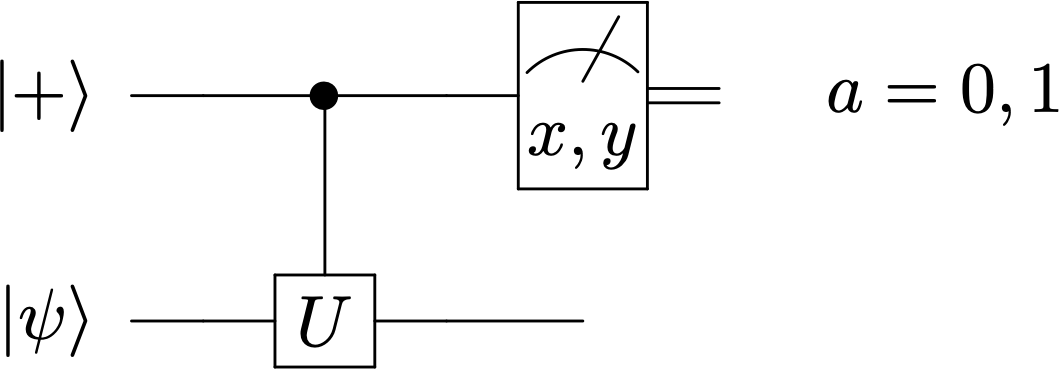
\includegraphics[width=0.3\linewidth]
	{Figuras/Fig_medidas2_Hadamard_measure}}
	\\
	\subfigure[Con el medidor $X$ expandido \label{Fig_medidas2_Hadamard_measurea}]{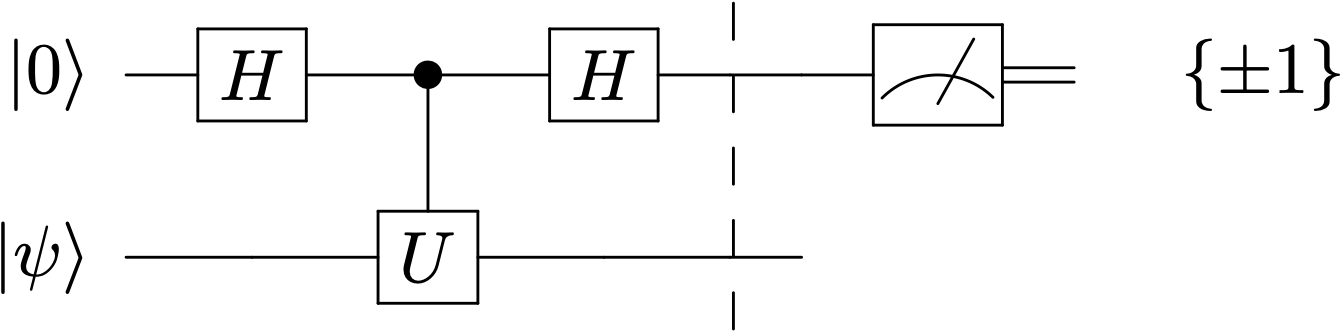
\includegraphics[width=0.4\linewidth]
	{Figuras/Fig_medidas2_Hadamard_measurea}} \hspace{2cm}
	\subfigure[Con el medidor $Y$ expandido \label{Fig_medidas2_Hadamard_measureb}]{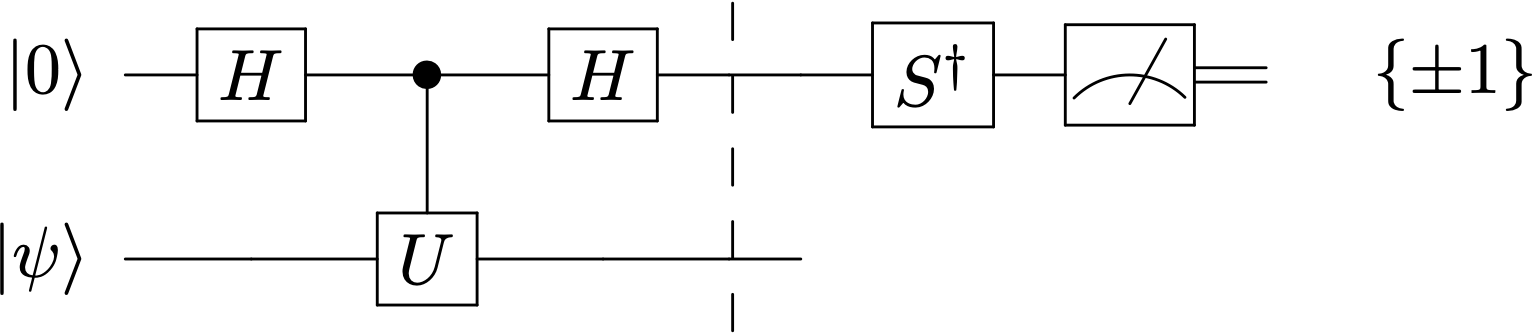
\includegraphics[width=0.4\linewidth]
	{Figuras/Fig_medidas2_Hadamard_measureb}}
	\caption{Medidas de Hadammard}
	\end{figure}
	}

	\begin{proof}
	 Para el caso $X$, el circuito anterior será el de la Fig. \ref{Fig_medidas2_Hadamard_measurea}. Un cálculo explícito nos da el estado que llega al aparato de medida (el estado que llega a las lineas punteadas verticales)
	$$
	\ket{0}\ket{\psi} ~\to ~ \ket{\Psi} = \frac{1}{2} \Lc \rule{0mm}{3mm} |0\rangle \otimes (1 + U) |\psi\rangle +  |1\rangle \otimes (1 - U) |\psi\rangle \Rc \label{hadam}
	$$
Si medimos el qúbit ancilla (el de arriba), obtendremos como resultados $\{0,1\}$ con probabilidades 
\begin{eqnarray} 
 p_{0}  &=&  \left\vert \frac{1}{2}  (1 + U) \ket{\psi}  \right\vert^{2} = 
 \frac{1}{4}\bra{\psi}(1 + U^\dagger) (1 + U) \ket{\psi} =\frac{1}{2}(1+\operatorname{Re}\langle \psi|U|\psi\rangle) \nonumber\\
 p_{1}  &=&  \left\vert \frac{1}{2}  (1 - U) \ket{\psi}  \right\vert^{2}=
 \frac{1}{4}\bra{\psi}(1 - U^\dagger) (1 - U) \ket{\psi} =
 \frac{1}{2}(1-\operatorname{Re}\langle \psi|U|\psi\rangle) \nonumber
\end{eqnarray}
El valor esperado $\langle X \rangle_{ancilla}$ será
	$$
	\langle X \rangle_{ancilla} = (+1) \frac{n^x_0}{n_0^x+n_1^x} + (-1) \frac{n^x_1}{n^x_0+n^x_1} =  \hbox{Re}\bra{\psi} U \ket{\psi}
	$$
La demostración para la medida en de $\ket{Y}$ y la obtención de la $\operatorname{Re}\langle \psi|U|\psi\rangle$ es análoga.
	\end{proof}

	\Ejercicio{
	Verificar que la parte imaginaria viene de medir  $\langle Y\rangle$ en la ancilla
	$$
	\langle{Y}\rangle_{ancilla}  =  \hbox{Im}\bra{\psi} U \ket{\psi} \, .
	$$
	}

Vemos que aquí estamos usando el poder del entrelazamiento, pues midiendo en un qubit que\textbf{ no tiene el estado} $\ket{\psi}$ \textbf{ni se ha aplicado el operador} $U$, somos capaces de calcular $\langle U \rangle_\psi$. 

	\begin{mybox_blue}{Nota: operadores hermíticos}
	Si estamos en el caso en que $U$ es hermítico, entonces solo hace falta medir $\langle X \rangle$, pues 
	los operadores hermíticos tiene todos sus autovalores reales.
	\end{mybox_blue}

	\Ejercicio{
	Define una función add\_Hadamadar\_measure que reciba un circuito y una  cadena de Pauli y añada al 
	circuito el medidor de Hadamard asociado.
	}
	
	\begin{mybox_orange}{Jypyter Notebook: 04-Medidas\_II seccion 4}
	Ver la sección 4 del notebook \textbf{04-Medidas\_II}.
	\end{mybox_orange}

        \subsection{Proyeccion de Hadamard}

Supongamos el operador $U$ es un operador sobre 1 qúbit \textbf{a la vez hermítico y unitario}. Por tanto puede ser considerado, a la vez, 
\begin{itemize}
	\item un observable con autovalores reales  $\lambda = \pm1$ y 
	\item una puerta cuántica con autovalores de módulo unidad
\end{itemize}
Ello deja a $\lambda = \pm 1$ como los únicos autovalores posibles para un operador así. Los operadores $X,Y,Z$ y $H$ son ejemplos de ello. 

Denominemos $\ket{a}_U, \, a=0,1$  los autovectores de $U$ con autovalores $(-1)^a$, es decir $U\ket{a}_U = (-1)^a\ket{a}_U$. En este caso, los factores $(1\pm U)$ que aparecen en la medida de Hadamard son proyectores ortogonales sobre los autoestados de $U$. La imagen bajo este circuito de un estado de entrada $\ket{0}\ket{\psi}$ ahora será
	\begin{equation}
	\ket{0}\ket{\psi} = \ket{0}\otimes (\alpha\ket{0}_U + \beta\ket{1}_U) ~~\longrightarrow ~~  \alpha\ket{0}\ket{0}_U +  \beta\ket{1}\ket{1}_U\, .
	\end{equation}
Podemos ver esto en la Fig. \ref{Fig_medidas2_HadamardProjection}  Al igual que con los estados de Bell, cada resultado de  medida en la ancilla está correlacionado con un autoestado del operador $U$.

	\begin{figure}[H]
	\centering 
	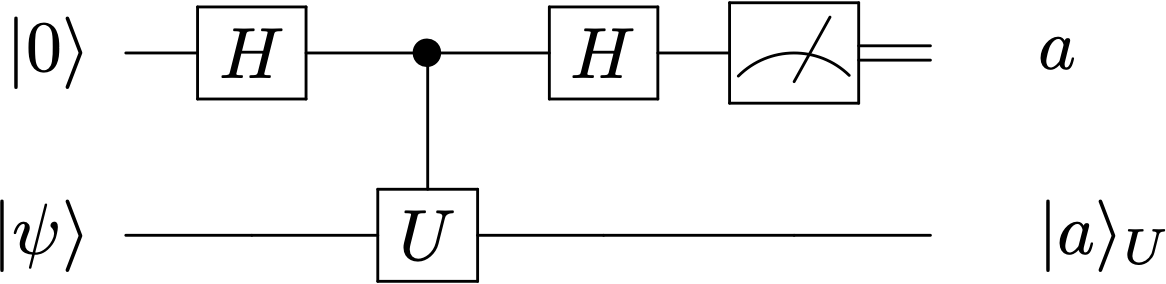
\includegraphics[width=0.4\linewidth]{Figuras/Fig_medidas2_HadamardProjection}
	\caption{Proyección de Hadammar}
	\label{Fig_medidas2_HadamardProjection}
	\end{figure}




















\chapter{Entrelazamiento en acción}

    \section{Desigualdades de Bell}

Con el nacimiento de la Mecánica Cuántica de mano de grandes físicos como Schrödinger o Dirac, también nacieron sus detractores. Uno de los más emblemáticos es el archiconocido Albert Einstein. Estos detractores defendían que la Mecánica Cuántica era una teoría incompleta. El argumento se basaba en que toda esta ``parafernalia'' de la Cuántica de las superposiciones, las indeterminaciones, el colapso de los estados,$\dots$ no eran más que consecuencia de tener una teoría incompleta. 

Argumentaban así que había \textbf{variables ocultas}, es decir, variables que no conocíamos pero en el caso de que las conociéramos, la Cuántica sería una teoría \textbf{determinista} (como la Mecánica Clásica). En esta batalla entre dos bandos enfrentados, entre los aférrimos defensores del determinismo (del \textbf{realismos local}) y los defensores de la cuántica, el tiempo y los experimentos dieron la razón a los segundos: la física cuántica no es una teoría determinista y no hay variables ocultas.

En este capítulo vamos a explicar el argumento que dio el golpe final a las variables ocultas y demostró el no determinismo inherente a la cuántica: \textbf{la violación de las desigualdades de Bell}.

Para ello, empecemos viendo un poco en detalle a que nos referimos cuando hablamos de \textbf{realismo local}. Las teorías con realismo local asumen que los valores que adquieren las magnitudes que se miden en un experimento \textbf{pertenecen} al sistema medido. Así, en una teoría con realismo local la posición de una partícula es algo bien definido aunque no la estemos midiendo\footnote{En una teoría con realismo local, si un árbol cae en el bosque este hace ruido aunque nadie lo escuche.}. La palabra \textbf{local} hace referencia a que ningún agente puede propagar su acción a mayor velocidad que la luz. Podría usarse la palabra \textbf{causal} en su lugar. 

Con esta definición en mente, tanto la Mecánica Clásica como un teoría cuántica con varibles ocultas serían teorías con realismo local. Sin embargo, la Mecánica Cuántica no lo sería. Cuando hablamos del espín de un electrón, no es correcto decir que \textbf{la proyección del espín a lo largo del eje $\hat{\bf z}$ es $+\hbar/2$}. Lo correcto es decir que, \textbf{al medir} la proyección sobre el eje $\hat{\bf z}$, la medida obtenida es $+\hbar/2$.  Dicho de otro, cualquiera de los valores $\pm\hbar/2$ se \textbf{adquiere} o \textbf{pone de manifiesto}  de forma \textbf{aleatoria} al hacer una medida de la proyección elegida.

En 1964  físico nor-irlandés John Bell, trabajando en el CERN demostró \cite{Bell} que \textbf{todas las teorías que respetan el realismo local} satisfacen ciertas desigualdades matemáticas. En particular, todas las magnitudes que evolucionan siguiendo las leyes de la física clásica las satisfacen.

Por el contrario, John Bell mostró cómo, en Mecánica Cuántica, el proceso de medida incorpora correlaciones sutiles que permiten \textbf{traspasar} dichas desigualdades. La discusión, pasó de ser puramente filosófica a ser objeto de investigación experimental, culminando con el  experimento de Alain Aspect y colaboradores en 1982 \cite{Bell_experiment}. Se observó que la Mecánica Cuántica viola las desigualdades de Bell y, por tanto, \textbf{no es una teoría con realismo local}: \textbf{las propiedades no pertenecen al sistema, se generan en la interacción entre el sistema y el medidor}.

La propuesta de John Bell dio pie a una familia de desigualdades que ponen en evidencia la imposibilidad de obtener ciertas correlaciones en un mundo clásico. Vamos a examinar la desigualdad en la forma estudiada por Clauser, Horne, Shimony y Holt (\textbf{CHSH}) \cite{Bell_CHSH}. Posteriormente estudiaremos el \textbf{experimento de GHZ}, el cuál, también pone de manifiesto las correlaciones sutiles que introduce el entrelazamiento de una forma determinista, en lugar de estadística.

    
        \subsection{Perfecta anticorrelación}

Central en esta discusión es la presencia de entrelazamiento. Vamos a seleccionar el denominado \textbf{singlete} de la Base de Bell. 
	\begin{equation}
	\ket{B_{11}}=\frac{1}{\sqrt{2}}(\ket{01}-\ket{10})
	\end{equation}
Una de las partículas del par entrelazado estaría en poder de Alice y la otra en poder de Bob. 

	\begin{mybox_blue}{Nota: creación del singlete}
	Desde un punto de vista experimental, para obtener este par entrelazado de electrones lo que se haces es coger los productos
	de una desintegración. Hay desintegraciones radioactivas que emiten estos pares entrelazados de electrones en direcciones 
	opuestas. 	
	\end{mybox_blue}

Supongamos que  Alice y Bob poseen sendos medidores de Stern Gerlach apuntando en la dirección $\hat{\bf z}$. De esta forma, lo que miden es el espín en la dirección $z$. Tenemos pues que
	\begin{itemize}
		\item Si Alice registra +1 el estado colapsa a $\ket{01}$ y, por tanto, Bob solo podrá medir  $\, -1$
		\item Si Alice registra -1 el estado colapsa a $\ket{10}$ y, por tanto, Bob solo podrá medir  $\, +1$
	\end{itemize}
En definitiva hay una anticorrelación perfecta que se pone de manifiesto en el valor medio del producto de las medidas. Si las mediciones de Alice son $a_i=\pm 1$, las de Bob son $b_i=\mp 1$ respectivamente, con lo cual el valor medio
$$
\langle Z\otimes Z\rangle = \frac{1}{N}\sum_{i=1}^N a_i b_i =\frac{1}{N}\sum_{i=1}^N (-1) = -1
$$

	\begin{mybox_blue}{Nota: Veámoslo}
	Vamos a ver cómo la predicción teórica confirma este hecho. El estado $\ket{B_{11}}$ ya es autoestado 
	del observable asociado a dicha pareja
	$$
	Z\otimes Z \ket{B_{11}} = Z\ket{0}Z\ket{1} - Z\ket{1}Z\ket{0} = -\ket{01} + \ket{10} = -\ket{B_{11}}
	$$
	Y el valor esperado satura en este autovalor, con lo que, la probabilidad de medida es 1
	$$
	\langle Z\otimes Z\rangle = \bra{B_{11}}Z\otimes Z\,  \ket{B_{11}}  = -\braket{B_{11}}{B_{11}}= -1\, .
	$$
	\end{mybox_blue}

	
	\begin{mybox_blue}{Nota }
	Hasta aquí, no se observa nada cuántico. La anti correlación que hemos hallado parece natural y presente en un 
	experimento clásico hecho con una bolsa que contiene dos calcetines de dos colores: si Alice saca el blanco, 
	el que saca Bob tiene que ser negro.
	\end{mybox_blue}

La cosa se pone más divertida cuando los dos polarizadores de Stern Gerlach \textbf{no se orientan en la misma dirección}. Es decir, cuando medimos las proyecciones del spín en dos direcciones diferentes. El observable asociado ahora a la dirección $\hat{\bf n}$  será  $\hat{\bf n}\cdot \boldsymbol{\sigma}$. Aun así, los autovalores de este operador y, por ello, la proyección del espín seguirá siendo $\pm 1$. Como ya comentamos, da igual en que eje se mida, los valores de la proyección del espín que podemos medir son los mismos. Sin embargo, ahora el valor esperado cambia:

	\Teorema{El valor medio del producto de las proyecciones de espín a lo largo de sendos ejes $\hat{\bf m}$ y 
	$\hat{\bf n}$ viene dada por el coseno del ángulo $\theta$  que forman los  ejes de los dos detectores     
	$$
	\bra{B_{11}}(\hat{\bf m}\cdot \boldsymbol{\sigma}\otimes \hat{\bf n}\cdot \boldsymbol{\sigma})\ket{B_{11}}
	= -\cos \theta = - \hat{\bf m}\cdot \hat{\bf n}
	$$ \label{Teo_entrelazamiento_bell}}
	
	\Ejercicio{Prueba el resultado del teorema \ref{Teo_entrelazamiento_bell}}

Cuando los ejes son paralelos recuperamos la  anticorrelación, independientemente de la dirección
$$
-\hat{\bf n}\cdot \hat{\bf n} = - \cos 0 = -1 
$$
mucho más interesante es cuando las direcciones de los detectores de Alice y Bob no coinciden ($\hat{\bf n} \neq \hat{\bf m}$).



        \subsection{Desigualdad CSCH}

Enn 1970 Clauser, Horne, Shimony y Holt \cite{Bell_CHSH} propusieron una figura de mérito fácilmente accesible para verificar las desigualdades de Bell. La idea es que Alice y Bob pueden orientar sus detectores en \textbf{dos direcciones  arbitrarias} cada uno. Para alice Alice denotamos $\hat{\bf n}_A, \hat{\bf n}'_A$  y  para Bob $\, \hat{\bf n}_B, \hat{\bf n}'_B$. Los pasos a seguir son los siguientes:
\begin{enumerate}
	\item Alice y Bob seleccionan cada uno una orientación (de las dos posibles de cada uno), p. ej.  $\hat{\bf n}_A$ y $\hat{\bf n}'_B$, para sus detectores. 
	Hay cuatro parejas posibles dependiendo de que selecciones cada uno
	$$
	\begin{array}{c|c} {\rm Alice} & {\rm Bob} \\ 
	\hline \hat{\bf n}_A  &  \hat{\bf n}_B     \\ 
	\hat{\bf n}_A         &  \hat{\bf n}'_B    \\ 
	\hat{\bf n}'_A        &  \hat{\bf n}_B     \\ 
	\hat{\bf n}'_A        &  \hat{\bf n}'_B \end{array}
	$$

	\item Alice y Bob reciben un electrón cada uno de un par entrelazado en el estado $\ket{B_{11}}$

	\item Alice y Bob realizan la medida de la proyección del espín a lo largo del eje elegido y anotan el resultado de la medición $(a,b')=(\pm 1, \pm 1)$
	
	\item Repiten el paso anterior un número $i=1,..., N$ grande de veces, y con los datos obtenidos $(a_i,b_i)=(\pm 1, \pm 1)$
donde $i=1,...,N$ pueden reconstruir la cantidad
	$$
	 C(\hat{\bf n}_A, \hat{\bf n}'_B) = \frac{1}{N}\sum_{i=1}^N a_i b'_i ~\in~  [-1,1]
	$$
Esta vez, como miden en direcciones diferentes, los dos pueden medir el mismo valor, así que esta cantidad estará ente $-1$ y $+1$.

	\item Repiten todo el proceso anterior para las cuatro posibles orientaciones elegidas de forma aleatoria. Con las  $4N$ mediciones construyen la cantidad
	\begin{equation} \label{ec_entrelazamiento_bell_R}
	R = | C(\hat{\bf n}_A, \hat{\bf n}_B) +  C(\hat{\bf n}_A, \hat{\bf n}'_B) +  C(\hat{\bf n}'_A, \hat{\bf n}_B)-  
	C(\hat{\bf n}'_A, \hat{\bf n}'_B)|
	\end{equation}

\end{enumerate}

En un mundo clásico, supondríamos que los valores $a_i,b_i$ proceden de \textbf{valores predefinidos} para cada sistema individual, sobre el que efectuamos simplemente un promedio estadístico de muchos sistemas. Entonces podemos probar la \textbf{desigualdad de CSCH}:

	\Teorema{La desigualdad de CSCH afirma que 
	\begin{equation} \label{ec_entrelazamiento_CHSH_R}
	R \leq 2
	\end{equation}
	}
	
	\begin{proof}
	Es fácil ver que se cumple para cada colección $a_i,a'_i,b_i,b'_i \in \pm 1$ la desigualdad
	$$
	a_i (b_i +  b'_i) + a'_i (b_i -  b'_i) = \pm 2
	$$
	porque si $b_i +  b'_i=\pm 2$ entonces $b_i - b'_i=0$ y viceversa. Ahora podemos demostrar la desigualdad 
	\begin{eqnarray*}
	R &=& \lim_{N\to \infty}|\frac{1}{N} \sum_{i=1}^N \left( a_i b_i + a_i b'_i + a'_i b_i - a'_i b'_i\right) | \nonumber\\
	&=& \lim_{N\to \infty}\frac{1}{N}| \sum_{i=1}^N  \left( a_i (b_i +  b'_i) + a'_i (b_i -  b'_i)\right)| \nonumber\\
	&\leq &  \lim_{N\to \infty} \frac{1}{N} \sum_{i=1}^N  |\left( a_i (b_i +  b'_i) + a'_i (b_i -  b'_i)\right)| \ \nonumber\\
	&= &  \lim_{N\to \infty} \frac{1}{N} \sum_{i=1}^N  2 \ \nonumber\\
	&=& 2
	\end{eqnarray*}
	\end{proof}

La Mecánica Cuántica nos proporciona una respuesta teórica para $R$ que sólo depende de los ángulos relativos $\cos\theta_{AB} = \cos(\theta_A-\theta_B)= \hat{\bf n}_A\cdot \hat{\bf n}_B$.
	\begin{equation}
	R = | \cos\theta_{AB}  + \cos \theta_{A'B} + \cos \theta_{AB'}  - \cos \theta_{A'B'}|\, .
	\end{equation}

			\SubsubiIt{Ejemplo particular.}
			 
Ahora sólo hace falta jugar un poco con los detectores. Por ejemplo, podemos situarlos en el plano $(y,z)$, perpendicular al eje de propagación $x$, de manera que los vectores  $\hat{\bf n}'_A,\hat{\bf n}_{A},\hat{\bf n}_B$ y $\hat{\bf n}_B'$ estén ordenados correlativamente en sentido horario. Finalmente tomaremos dos ejes coincidentes $\hat{\bf n}_{A}=\hat{\bf n}_B$ paralelos $\Rightarrow \theta_{AB}=0$, y apertura igual para ambos, $\theta_{A'A} = \theta_{BB'} = \varphi$, de modo que $\theta_{A'B'} = 2\varphi$. Podemos ver esta disposión en la Fig. \ref{Fig_entrelazamiento_CHSH_basis}.

	\begin{figure}[t]
	\centering 
	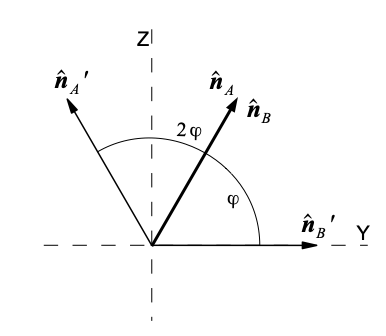
\includegraphics[width=0.35\linewidth]{Figuras/Fig_entrelazamiento_CHSH_basis}
	\caption{Ejemplo particular de unas orientaciones de los medidores de Alice y Bob}
	\label{Fig_entrelazamiento_CHSH_basis}
	\end{figure}

La expresión de $R$ nos queda
$$
R = |1 +  2 \cos\varphi  - \cos 2\varphi|\, .
$$
Derivando vemos que esta expresión alcanza su máximo cuando $\sin\varphi = \sin 2\varphi$ lo cual tiene solución $\varphi = \pi/3 = 60^\circ$. Sustituyendo encontramos $R= 2.5>2$, violando la desigualdad CHSH de la Ec. (\ref{ec_entrelazamiento_CHSH_R}).

	\begin{mybox_orange}{Jypyter Notebook: 05-Entrelazamiento sección 1}
	Ver la sección 1 del notebook \textbf{05-Entrelazamiento}.
	\end{mybox_orange}
	
	\Ejercicio{Prueba con otros estados de la base de Bell. Realiza este experimento en un ordenador real.}
	
	\Ejercicio{Usar bases perpendiculares de  Alice $A$ y $A'$  y Bob $B$ y $B'$, y formando un ángulo $\varphi$ entre sí. Sin pérdida de generalidad puedes tomar $B = X$ y $B' = Z$. Variar $\varphi$ en el intervalo $(0,\pi)$ y hallar el valor de la máxima violación de la desigualdad de Bell.}

    \section{Experimento GHZ}

Las desigualdades de Bell-CHCS demuestran que hay una manera de distinguir una teoría con  realismo local de una en la que este postulado no  exista. Lo hacen de una forma estadística: es necesario tormar ciertas medias de datos sobre estados de 2-cúbits, los  estados de Bell. Vamos a ver ahora una forma alternativa de llegar a la misma conclusión, pero esta vez de una forma \textbf{determinista}, no probabilística.

Supongamos un sistema, compuesto de  tres subsistemas, $A, B$ y $C$. En cada uno de ellos hay dos \textbf{magnitudes} observables, $X$ e $Y$, que al ser medidas adquieren valores binarios $x, y = \pm 1$. Pretendemos saber si existe un estado del sistema tal que, con el resultado  de  medidas simultáneas $X$ o $Y$ de cada una de sus partes $A,B$ y $C$ , se obtengan resultados $x$ e $y$ que verifiquen las siguientes ecuaciones:

$$
\begin{array}{ccc}
{\rm medimos} & & \hbox{obtenemos} ~ x,y ~~ \hbox{tales que} \\
XYY ~~~~~ &\to& ~xyy =~~~ 1\nonumber\\
YXY ~~~~~ &\to& ~yxy =~~~ 1 \\
YYX ~~~~~ &\to& ~yyx =~~~ 1\nonumber\\
XXX ~~~~~ &\to& ~xxx = -1\nonumber
\end{array}
$$

Si la teoría satisface los axiomas de realismo local,  los valores de $X$ es $Y$ estarán bien definidos independientemente de la medida que efectuemos. Dicho de otra forma, las medidas que efectuamos son compatibles y no afectan a los resultados posibles. Entonces podemos utilizar conclusiones que extraigamos de los resultados de un experimento para los de otro (notar que se supone que el estado es el mismo en todos los casos)
\begin{itemize}
	\item Las tres primeras afirman que $x=1$ puesto que $y^2=1$. 
	\item La última afirma que $x=-1$
\end{itemize}
vemos que hay una contradicción. Concluímos que las medidas efectuadas \textbf{no son compatibles entre sí}. Como vemos, la paradoja existe en tanto en cuanto atribuyamos a las magnitudes $X$ e $Y$ una noción de realidad  independiente de la medición. Es decir, cuando pensamos desde la perspectiva del realismo local en la que los valores de $x$ e $y$ están predefinidos y el hecho de medir no los altera. 

Concluimos que para que se cumplan las 4 afirmaciones tenemos que aceptar que las variables $X$ e $Y$, no pueden tener valores predefinidos simultáneamente  en los cuatro experimentos. La pregunta ahora es, hay algún estado cuántico que si cumpla esas 4 condiciones? La respuesta es sí, el estado GHZ.

En 1997 Greenberger, Horne y Zeilinger estudiaron las propiedades de una serie de estados de 3-qúbits.   Consideremos el siguiente estado entrelazado
	\begin{equation} \label{ec_medidad_GHZ}
	\ket{\rm GHZ} = \frac{1}{\sqrt{2}}( \ket{000} - \ket{111} )\, . 
	\end{equation}
Este estado se denomina \textbf{estado GHZ}. Cuánticamente es fácil ver que el estado GHZ proporciona una solución al conjunto de ecuaciones. Supongamos que  $x$ e $y$ son los resultados de aplicar $X = \sigma_x$ y $Y = \sigma_y$, los operadores hermíticos  usuales que miden la componente del espín
$$
X \ket{0} = \ket{1}\, , ~ X \ket{1} = \ket{0}\, , ~ Y \ket{0} = i \ket{1}\, , ~ Y \ket{1} = -i \ket{0}\, . ~ 
$$
Por un lado, 
$$xyy\ket{{\rm GHZ}}  = X \otimes Y\otimes Y \big(\frac{1}{\sqrt{2}}(\ket{000}-\ket{111}\big) = \frac{1}{\sqrt{2}} \big(i^2 \ket{111}- (-i)^2
\ket{000}\big) = +  \ket{{\rm GHZ}}\, ,$$
y, análogamente, obtenemos $xyy=yxy=yyx= +1$. Por otro, $xxx=-1$ se sigue de
$$  
xxx  \ket{{\rm GHZ}} =   X \otimes X \otimes X \big(\frac{1}{\sqrt{2}}(\ket{000}-\ket{111}\big) =
\frac{1}{\sqrt{2}}(\ket{111}-\ket{000}) =  - \ket{\rm GHZ}\, .
$$

Podemos ver en la Fig. \ref{Fig_entrelazamiento_GHZ} el circuito que genera el estado GHZ de la Ec. (\ref{ec_medidad_GHZ}). 

	\begin{figure}[H]
	\centering 
	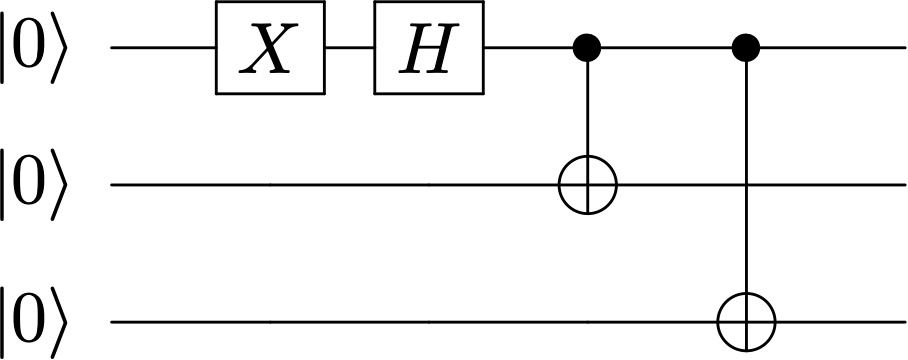
\includegraphics[width=0.4\linewidth]{Figuras/Fig_entrelazamiento_GHZ}
	\caption{Circuito que genera el estado GHZ de la Ec. (\ref{ec_medidad_GHZ})}
	\label{Fig_entrelazamiento_GHZ}
	\end{figure}


	\begin{mybox_orange}{Jypyter Notebook: 05-Entrelazamiento sección 2}
	Ver la sección 2 del notebook \textbf{05-Entrelazamiento}.
	\end{mybox_orange}



    \section{Teleportación}



El entrelazamiento conlleva un tipo  nuevo de correlación que acaba constituyendo un recurso importante.  Podemos usar esta correlación para \textbf{teleportar} estados. Lo primero que debemos entender es que cuando hablamos de ``teleportar'' estamos hablando de \textbf{teloportar un estado cuántica}. Es decir, no estamos teleportando un partícula, sino que estamos aprovechando el entrelazamiento para transferir el estado de una partícula a otra. Como las partículas de la misma clase (como los electrones) son indistinguibles, si conseguimos teleportar  el estado de una partícula a otra, a efectos prácticos es como si teleportaramos la partícula en si. 

       
Supongamos que Alice y Bob tiene dos qúbits que se encuentran en el estado entrelazado $\ket{B_{00}}$.  Alice tiene, un segundo qúbit inicializado en un estado arbitrario $\ket{\phi}$, y se plantea la posibilidad de transferirlo o clonarlo en el laboratorio de Bob. El circuito de la Fig. \ref{Fig_entrelazamiento_teleportacion} permite efectuar esa tarea

	\begin{figure}[H]
	\centering 
	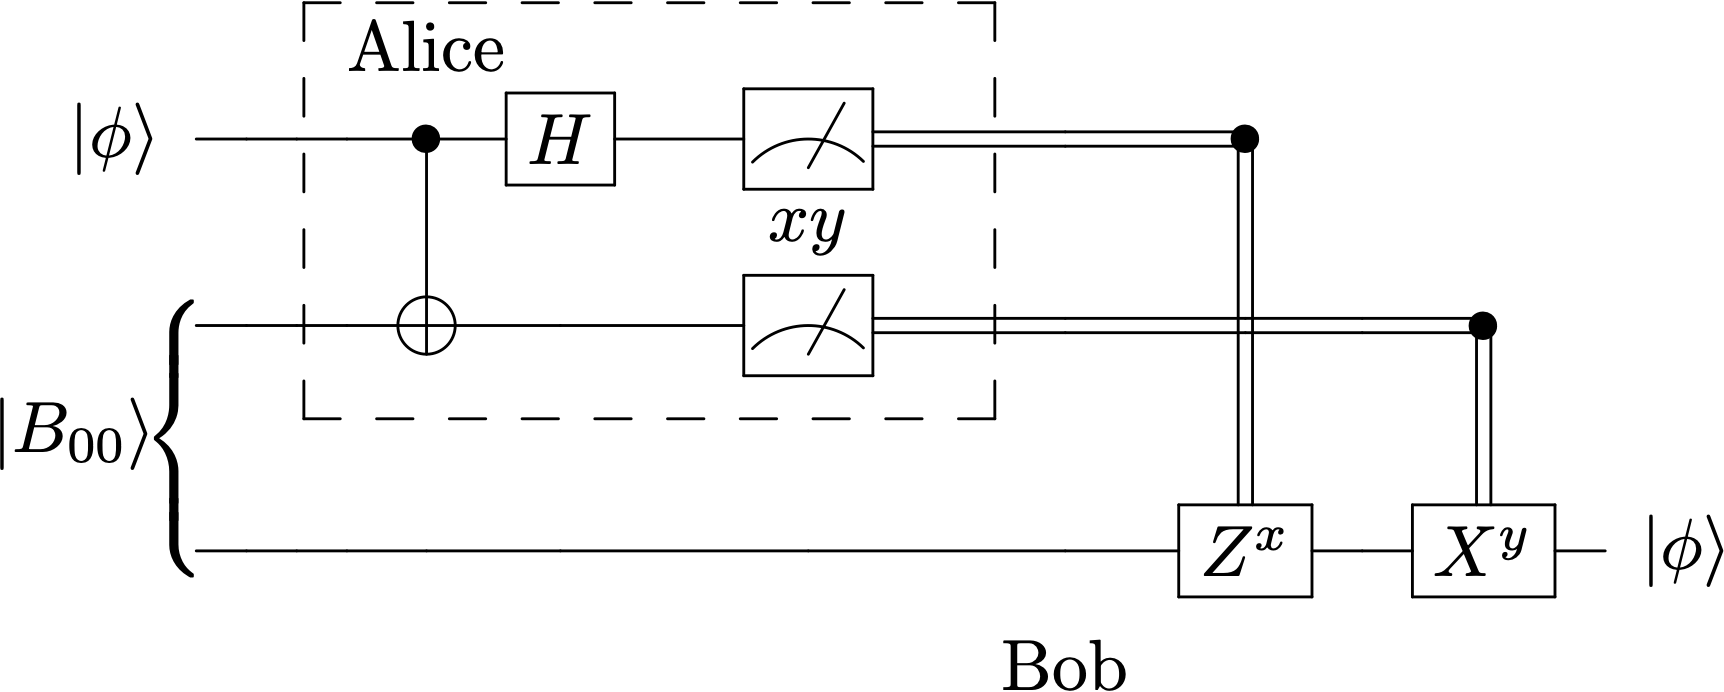
\includegraphics[width=0.45\linewidth]{Figuras/Fig_entrelazamiento_teleportacion}
	\caption{Circuito del protocolo de teleportación.}
	\label{Fig_entrelazamiento_teleportacion}
	\end{figure}

\begin{enumerate}
	\item El estado inicial es
$$ 
\ket{\phi} \ket{B_{00}} =  \ket{\phi}\otimes \frac{1}{\sqrt{2}}\left(\ket{0}\otimes \ket{0} + \ket{1}\otimes\ket{1}\rule{0mm}{4mm}\right)\, .
$$
Alice tiene acceso a los dos primeros qubits y Bob al tercero. El estado que queremos teleportar es $\ket{\phi}$. De forma genérica, este estado será de la forma
$$
\ket{\phi} = a \ket{0} + b \ket{1}
$$

	\item Alice realiza una  \textit{medida de Bell} a sus dos qúbits.
Ello  implica un desentrelazador $U_{\rm desent}= (H \otimes I)\cdot U_{\rm CNOT}.~$
Un cálculo sencillo  da el resultado
	\begin{align*} 
	(H \otimes I\otimes I)(U_{\rm CNOT}\otimes I)\, \ket{\phi}\ket{B_{00}}  = &  \frac{1}{2}
	\Lc \rule{0mm}{3mm} \ket{00}(a\ket{0} + b\ket{1}) + \ket{01}(a\ket{1}+ b\ket{0}) \R. \\
	\rule{0mm}{6mm}
	&\L.  \rule{0mm}{3mm}+ ~\ket{10}(a\ket{0}-b\ket{1}) + \ket{11}(a\ket{1}-b\ket{0}) \Rc
	\end{align*}
	Podemos ver que al estar entrelazados, las operaciones sobre los qúbit de Alice afectan al estado del qúbit de Bob. 

	\item Alice mide el estado que obra en su poder, y obtiene un 2-bit  clásico, $xy$ de manera equiprobable para las 4 posibilidades. De forma correlacionada, el qúbit de Bob colapsa a uno de los 4 estados $\ket{\varphi_{xy}},$ pero no sabe a cuál. 

	\item Alice envía el resultado de su medida $xy$ por un canal clásico a Bob.
	
	\item Bob efectúa sobre su qúbit, una operación controlada por este 2-bit, $U_{xy} =  X^y Z^x $. 
$$
xy ~=~ \left\{ \begin{array}{c} 00 \\ 01 \\ 10 \\ 11 \end{array} \right\}~~ \Longrightarrow  
~~~ X^y Z^x \ket{\varphi_{xy}} ~=~ \left\{  \begin{array}{rl}    I :& (a\ket{0} + b\ket{1})  \\    X: & (a\ket{1} + b\ket{0})  \\  Z:& (a\ket{0} - b\ket{1})  
\\  XZ = -iY:&   (a\ket{1} - b\ket{0}) \\
       \end{array} \right. ~~ \longrightarrow  ~~ a \ket{0} + b\ket{1}\,  = \, \ket{\phi}
$$
Como resultado de esta operación, el qúbit de Bob es finalmente $\ket{\phi}$.

\end{enumerate}

	\Ejercicio{Calcula $(H \otimes I\otimes I)(U_{\rm CNOT}\otimes I)\, \ket{\phi}\ket{B_{00}}$ y verifica que la ecuación del paso 2 es correcta.}

	\begin{mybox_orange}{Jypyter Notebook: 05-Entrelazamiento sección 3}
	Ver la sección 3 del notebook \textbf{05-Entrelazamiento}.
	\end{mybox_orange}
	
El siguiente ejercicio ilustra el principio de la medida diferida.	
	
	\Ejercicio{Modifica y ejecuta  el circuito de teleportación de dos formas distintas
	\begin{itemize}
		\item[a)] sustituyendo los controles clásicos por controles cuánticos
		\item[b)] permutando el orden de los controles y los aparatos de medida
	\end{itemize}
	Discute la sutileza que distingue estas posibilidades. 
	}
	
	\Ejercicio{Cambia el estado que comparten Alice y Bob por $\ket{B_{11}}$ y modifica el circuito para que teleporte igualmente.}

	\begin{mybox_blue}{Nota: causalidad y clonación.}
	El protocolo de teleportación parece poner en riesgo conceptos fundamentales. Sin embargo,
	no es así:
	\begin{itemize}
		\item \textbf{No clonación}: 
		
		El protocolo tiene como ingrediente esencial la medida y, por tanto, la 
		destrucción del estado de Alice. Como consecuencia, el estado ha sido teleportado
		pero no clonado.  De no ser así, entraríamos en conflicto con el  
		\textbf{Teorema de No Clonación}
		
		\item \textbf{Causalidad}: 
		
		El protocolo de teleportación \textbf{no viola causalidad}. Es necesario mandar 
		una información clásica (como muy rápido a la velocidad de la luz) para resolver la
		ambigüedad que le queda a Bob. Esta parte es la que hace que la teleportación no sea
		un proceso instantáneo de acción a distancia.    
    
	\end{itemize}
	\end{mybox_blue}

    
    \section{Intercambio de Entrelazamiento}

Ya hemos visto cómo el ejemplo más sencillo de entrelazamiento tiene una aplicación muy interesante en la teleportación. Vamos a ver que el entrelazamiento se puede ``contagiar'' a terceras partes. En inglés se denomina \textbf{entanglement swapping}.

Consideremos el circuito de la Fig. \ref{Fig_entrelazamiento_entanglement_swap}. El circuito podemos interpretarlo de la siguiente forma:
	\begin{enumerate}
		\item Alice (A) entrelaza un qúbit con Charles (C) y otro con Bob (B).
		
		\item Después, Alice hace una medida de Bell, y comunica el resultado $xy$ a Charles 
		y a Bob respectivamente.
		
		\item Charles y Bob efectúan las puertas controladas $Z^x$ y $X^y$ respectivamente. El resultado final es que los qúbits de Bob y Charlie están entrelazados.
	\end{enumerate}


	\begin{figure}[H]
	\centering 
	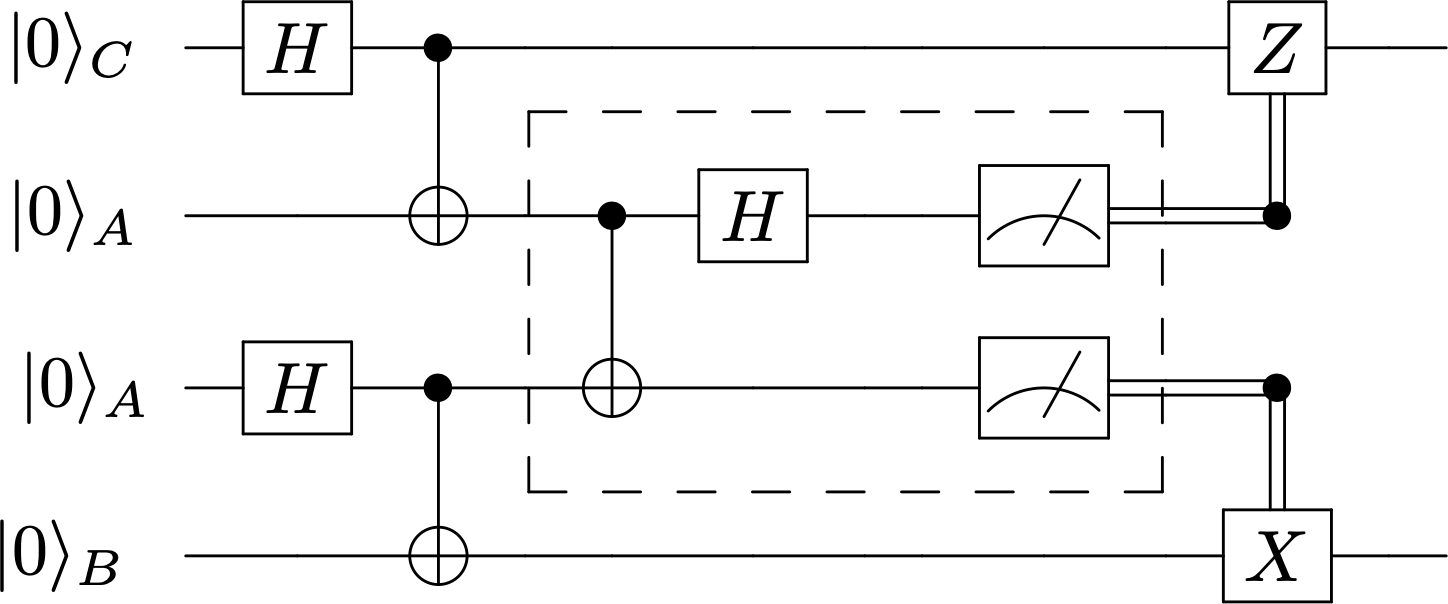
\includegraphics[width=0.45\linewidth]{Figuras/Fig_entrelazamiento_entanglement_swap}
	\caption{Circuito para el intercambio de entrelazamiento (entanglement swapping)}
	\label{Fig_entrelazamiento_entanglement_swap}
	\end{figure}


	\Ejercicio{Completa los siguientes apartados:
	\begin{itemize}
	\item[a)] Programa el circuito de la Fig. \ref{Fig_entrelazamiento_entanglement_swap}.
	\item[b)] Ejecuta varias veces el circuito y muestra que el estado final que comparten Bob y Charles está entrelazado. ¿Es siempre el mismo estado?
	\end{itemize}}
	
	\Ejercicio{A partir del circuito de la Fig. \ref{Fig_entrelazamiento_entanglement_swap}, diseña y ejecuta un protocolo capaz de teleportar un qúbit arbitrario entre Charles y Bob.}


	\section{Teorema de no-clonación} \label{sec_no_clone}
	
	En un principio, que el protocolo de teleportación exija la destrucción del estado inicial para teleportarlo puede parecer una particularidad de este protocolo. Sin embargo, nada más lejos de la realidad.
	El \textbf{Teorema de No Clonación} es uno de los resultados más sencillos y a la vez más importante del formalismo de la Mecánica Cuántica. De hecho su formalización completa es bastante reciente, 1982, debida a Wootters, Zurek \cite{clone2} y Dieks \cite{clone1}.
	
	\Teorema{ \textbf{(de No Clonación)} No existe un operador unitario $U$ (clonador) que, para un estado arbitrario $|\psi\rangle$, realice la siguiente operación
		\begin{equation}
		U \ket{\psi}\ket{0} = \ket{\psi}\ket{\psi}
		\end{equation}}

	\begin{proof}
	Supondremos que $U$ existe y llegaremos a una contradicción. 
	Tratemos de clonar el estado $\alpha\ket{\psi}+\beta\ket{\phi}$. Esto implica evaluar
		\begin{equation*}
		U (\alpha\ket{\psi}+\beta\ket{\phi})\otimes \ket{0} = 	(\alpha\ket{\psi}+\beta\ket{\phi})\otimes (\alpha\ket{\psi}+\beta\ket{\phi})
		\end{equation*}	
	Sin embargo, la linealidad de $U$ nos permite seguir otro camino
		\begin{align*}
		U(\alpha|\psi\rangle+\beta|\phi\rangle) \otimes|0\rangle 
			& = \alpha U|\psi\rangle \otimes|0\rangle+\beta U|\phi\rangle \otimes|0\rangle  \\
			& = \alpha|\psi\rangle \otimes|\psi\rangle+\beta|\phi\rangle \otimes|\phi\rangle . 
		\end{align*}
	Los dos resultados son diferentes y el teorema queda demostrado por reducción al absurdo.
	\end{proof}


	\begin{mybox_blue}{Nota}
	\begin{itemize}
		\item El teorema de no clonación pone  de manifiesto la  \textit{tensión} que hay entre linealidad y tensorialidad cuando se trata de aplicar operadores.
		\item Es muy importante recalcar que la validez de este teorema sólo aplica a estados \textit{genéricos}. 
	Si por ejemplo nos restringimos a estados de la base $\ket{0}$ y $\ket{1}$, entonces la mera puerta CNOT es un operador de clonación.
    $$
	\cg{X}\ket{00}\to \ket{00}~~~~~,~~~~~~ \cg{X}\ket{10}\to \ket{11}
	$$
	\end{itemize}		 
	\end{mybox_blue}









\chapter{Hardware: Técnicas de control y computación en RMN.}

En este capítulo vamos a ver un poco más en detalla como se implementa un computador cuántico. En concreto, veremos de manera relativamente profunda el formalismo detrás del control de los qúbits en \textbf{RMN} (Resonancia Magnética Nuclear). Esto es debido a que, a pesar de que actualmente las implementaciones de los qúbits son variopintas, la teoría detrás del control de los qúbits es más o menos igual. 

	\section{Introducción.}

El problema del control de sistemas cuánticos acoplados múltiples es un tema emblemático de la RMN, y puede resumirse como sigue: dado un sistema con Hamiltoniano
\begin{equation}
\mathcal{H} = \mathcal{H}_{sys} + \mathcal{H}_{control}
\end{equation}
donde $\mathcal{H}_{sys}$ es el Hamiltoniano del sistema en ausencia de cualquier control, y $\mathcal{H}_{control}$ describe términos que están bajo control externo, ¿cómo puede aplicarse una transformación unitaria $U$ deseada, en presencia de imperfecciones y utilizando un mínimo de recursos? De forma similar a otros escenarios en los que el control cuántico es una idea bien desarrollada, como en la excitación láser de reacciones químicas, $\mathcal{H}_{control}$ \textbf{surge de secuencias sincronizadas con precisión de múltiples pulsos de radiación electromagnética, aplicados de forma coherente en fase, con diferentes anchuras, frecuencias, fases y amplitudes de pulso.}

En RMN lo que se controla con esto pulsos es el \textbf{espín nuclear}. Tenemos que ver entonces que es el espín nuclear (sección \ref{sec_sub_Harware_NMR_espin}), como se puede usar para formar qúbits (construir $\mathcal{H}_{sys}$, sección \ref{sec_subsub_Harware_NMR_H_sys}) y como se  manipulan usando pulsos electromagnéticos (construir $\mathcal{H}_{control}$, sección \ref{sec_subsub_Harware_NMR_H_control}). Finalmente, veremos más en detalle como se implementan estos pulsos (sección \ref{sec_sub_Harware_NMR_pulsos}).

Para más información en general sobre física núclear, puede consultarse un libro clásico como es \cite{Krane:359790}. Para más información sobre como controlar qúbits de RMN puede consultarse \cite{NMR_hardware}. Gran parte de este capítulo se basa en intentar explicar de una forma más simple este último artículo.



		\section{El espín nuclear} \label{sec_sub_Harware_NMR_espin}

En el núcleo, cada nucleón (protones o neutrones) posee un momento angular orbital y un momento angular intrínseco o espín. Al igual que el electrón, los nucleones son fermiones de espín $\hbar/2$. 

A cada \textbf{estado nuclear} se asigna un único número cuántico de espín $I$, representando el \textbf{momento angular total} (orbital más intrínseco) de todos los nucleones en el núcleo. El vector $\vec{I}$ puede considerarse como la suma de las contribuciones orbital y intrínseca (espín intrínseco de protones y neutrones) de los momento angulares de los nucleones
\begin{align} \label{ec_Hardware_NMR_I}
\vec{I} ~ & =  ~ \, \sum_{i=1}^A (\vec{l_i} +  \vec{s_i}) \nonumber \\
& = ~ \,  \vec{L} + \vec{S}  \\
& = ~ \, \sum_{i=1}^A \vec{j_i} \nonumber
\end{align}
donde $A$ es el \textbf{número másico} 
	\begin{equation}
	A = Z + N 
	\end{equation}
donde $Z$ es el \textbf{número de protones} y $N$ el \textbf{número de neutrones}.

El \textit{número cuántico} $I$ tiene la conexión  usual con el \textit{vector} $\vec{I}$:
\begin{align}
| \vec{I} | ~ = & ~\,  \sqrt{I(I+1)} \hbar \\
I_i ~ = & ~\, m_i \hbar \qquad (m_i = I, I-1, \dots, -I +1, -I)
\end{align}
Al vector $\vec{I}$ se lo denomina \textbf{espín nuclear}.

	\begin{mybox_blue}{Nota: $S_z$ e $I_Z$}
	Aunque aquí hayamos decidido usar una notación difenciadora para el spín de una partícula 
	y un núcleo ($\vec{S}$ y $\vec{I}$), a partir de aquí \textbf{usaremos $\vec{S}$ para todo}.
	\end{mybox_blue}



	\begin{mybox_blue}{Nota: Operador de espín para partículas de espín 1/2}
	En física cuántica todos los observables son operadores (matrices hermíticas). Ya hemos visto 
	el vector de espín, $\vec{S}$ (o $\vec{I}$, pero ya comentamos que abandonamos esta notación),
	ahora nos falta ver el \textbf{operador espín},	$\hat{S}$ o simplemente $S$. Para partículas de 
	espín 1/2, este toma la forma
		\begin{equation} \label{ec_Hardware_NMR_operador_S_sigma_vec}
		\boxed{S = \frac{\hbar}{2} \vec{\sigma}}
		\end{equation}
	donde $\vec{\sigma}$ es el vector de matrices de Pauli $(\sigma_x, \sigma_y, \sigma_z)$.
	También podemos escribirlo pues como
		\begin{equation} \label{ec_Hardware_NMR_operador_S_vec_Sx-Sy-Sz}
		S = (S_x, S_y, S_z)
		\end{equation}
	donde 
		\begin{equation} \label{ec_Hardware_NMR_Sx-Sy-Sz}
		\boxed{S_x = \frac{\hbar}{2} \sigma_x} \, , \hspace{2cm} 
		\boxed{S_y = \frac{\hbar}{2} \sigma_y} \, , \hspace{2cm} 
		\boxed{S_z = \frac{\hbar}{2} \sigma_z} \, .
		\end{equation}
	\end{mybox_blue}
	
	\begin{mybox_blue}{Nota: Operador momento angular}
	Es común en física que se usen la notación $I = (I_x, I_y, I_z)$ para hablar del 
	\textbf{operador de momento angular}. No confundirlo con el espín nuclear que vimos
	antes. Este operador es simplemente el operador de espín (\ref{ec_Hardware_NMR_operador_S_sigma_vec})
	pero sin el factor $\hbar$, es decir,
		\begin{equation} 
		I = \frac{1}{2} \vec{\sigma}
		\end{equation}
	Por ejemplo, en el paper de referencia de esta sección \cite{NMR_hardware} se usa esta notación. 
	\end{mybox_blue}

La Ec. (\ref{ec_Hardware_NMR_I}) representa lo que en principio podría ser un acoplamiento muy complicado de muchos vectores para dar un solo resultado, y puede que no sea evidente por qué podemos despreciar esta estructura interna y tratar el núcleo como si fuera un momento angular una ``partícula''. Esto es posible porque las interacciones a las que sometemos el núcleo, como los campos electromagnéticos, no son suficientemente fuertes como para cambiar la estructura interna o romper los acoplamientos de los nucleones que son responsables de la Ec. (\ref{ec_Hardware_NMR_I}). 

El valor del espín nuclear depende del valor del número másico:
\begin{align*}
& \text{Núcleos con }A \text{ impar:} ~ \longrightarrow \text{Espín nuclear, } I \text{, semientero}   \\
& \text{Núcleos con }A \text{ par:} ~~~ \,\, \, \longrightarrow \text{Espín nuclear, } I \text{, entero}
\end{align*}
Esto es debido a que los nucleones tienden a acoplarse en parejas de iguales (pp y nn) con el mismo momento angular orbital pero con los espines opuestos, situación consistente con el principio de exclusión de Pauli y que minimiza la energía potencial del sistema permitiendo un mayor solapamiento de las funciones de onda de los nucleones. Teniendo esto en cuenta, es de esperar que usualmente las propiedades magnéticas nucleares estén determinadas por el último nucleón desapareado (si existe), por el acoplamiento de la última pareja de nucleones, ó por el acoplamiento del espín del nucleón desapareado con el espín del core nuclear residual (bastante similar a lo que ocurre con los electrones más externos de los átomos).

Todos los núcleos que se conocen (estables e inestables) con $Z$ par y $N$ par tienen espín cero en el estado fundamental. Lo cual es una evidencia de que la interacción fuerte manifiesta una especie de fuerza de apareamiento tal que existe una tendencia a mantener los nucleones apareados. Como consecuencia, resulta que el espín del estado fundamental de un núcleo con $A$ impar debe ser igual al $\vec{j_i} = \vec{s_i} + \vec{l_i}$ del protón o neutrón desapareado.


	
	\section{Qúbits de RMN} 

En esta sección vamos a describir como es el sistema con el que se construyen los qúbits en RNM, basándonos en su \textbf{Hamiltoniano del sistema} y su \textbf{Hamiltoniano de control}. El Hamiltoniano del sistema da la energía de los espines simples y acoplados en un campo magnético estático, y el Hamiltoniano de control surge de la aplicación de pulsos de radiofrecuencia al sistema en, o cerca de, sus frecuencias resonantes. Veremos que para describir el efecto de los pulsos es más conveniente usar un \textbf{sistema de referencia giratorio}.


		\subsection{Hamiltoniano del sistema} \label{sec_subsub_Harware_NMR_H_sys}


			\SubsubiIt{Espines simples.} 

Una partícula con espín constituye un \textbf{dipolo magnético}\footnote{En esencia, un pequeño imán, es decir, una fuente de campo magnético.}. El \textbf{momento dipolar magnético}, $\vec{\mu}$, es proporcional al momento angular de espín, $\vec{S}$:
	\begin{equation} \label{ec_Hardware_NMR_mu}
	\vec{\mu} = \gamma \vec{S}\, ,
	\end{equation}
donde la constate de proporcionalidad, $\gamma$, se denomina ratio giromagnético (\textbf{gyromagnetic ratio}). Este toma la forma
	\begin{equation} \label{ec_Hardware_NMR_gamma}
	\gamma = g \frac{q}{2m} \, ,
	\end{equation}
donde $q$ es la carga eléctrica de la partícula, $m$ su masa y $g$ se denomina \textbf{factor $g$ ($g$-factor)}. 

Cuando un dipolo magnético se sitúa en un campo magnético $\vec{B}$, este dipolo experimenta un torque, $\vec{\mu} \times \vec{B}$, que tiende a alinearlo paralelo al campo (como la aguja de una brújula). La energía asociada con este torque es
	\begin{equation}
		E = - \vec{\mu} \cdot \vec{B}
		\end{equation}	
con lo que el Hamiltoniano para una partícula cargada con espín, en reposo en un campo magnético $\vec{B}$, es
	\begin{equation}
	\mathcal{H} = - \gamma \vec{B} \cdot S
	\end{equation}
donde $S$ es el operador de espín (ver Ec. (\ref{ec_Hardware_NMR_operador_S_sigma_vec}) para el caso de partículad de espín 1/2).

Si tenemos una partícula (o un núcleo) de espín 1/2 (no consideraremos espines de mayor orden en estas notas) en un campo magnético $\vec{B}_0$ a lo largo del eje $\hat{z}$, entonces su evolución temporal está gobernada por el Hamiltoniano
	\begin{equation} \label{ec_Hardware_NMR_H_sys_1}
	\boxed{\mathcal{H} = -  \gamma B_0 S_z = - \omega_0 S_z = 
	\begin{bmatrix}
	- \hbar \omega_0/2  & 0 \\
	0  &  \hbar \omega_0 /2
	\end{bmatrix}} \, ,
	\end{equation}
donde 
\begin{itemize}
	\item $\gamma$ es ratio giromagnético del núcleo (ver Ec. (\ref{ec_Hardware_NMR_gamma})),
	\item $\omega/2 \pi = \gamma B_0 $ es la \textbf{frecuencia de Larmor}\footnote{En Física, la \textbf{frecuencia} se define como el inverso del periodo de rotación: $f = 1/T$ y se mide en Hz (1/segundos). Además, se define la \textbf{frecuencia angular} como $\omega = 2\pi f$ y se mide en radianes/segundo. Muchas veces se denomina a las dos, simplemente, frecuencia.}
	\item e $S_z$ es el operador de espín en la dirección $\hat{z}$ (ver Ec. (\ref{ec_Hardware_NMR_Sx-Sy-Sz})).
\end{itemize}

La interpretación de la Ec. (\ref{ec_Hardware_NMR_H_sys_1}) es simple. Cuando tenemos una partícula de espín 1/2 aislada, las dos proyecciones del espín son \textbf{degeneradas}, es decir, tiene la misma energía. Esto es fácil de entender si pensamos en que no hay ninguna dirección privilegiada en el sistema. Cuando introducimos un campo magnético, ahora sí hay una dirección privilegiada: aquella con el momento dipolar magnético $\vec{\mu}$ apuntando en la misma dirección que el campo magnético. Esto es debido a que el espín es como un pequeño imán y tiende a orientarse con el campo magnéticos. En este momento, el sistema pasa a ser \textbf{no-degenerado}, y un estado tiene más energía que el otro.

Esto último se traduce matemáticamente en la Ec. (\ref{ec_Hardware_NMR_H_sys_1}). Como el Hamiltoniano es diagonal, los elementos de la diagonal son las energías de los estados. Vemos que el estado con el espín apuntando en la misma dirección (es estado $\ket{0}$ o $\ket{\uparrow}$) que el campo magnético tiene menos energía que el estado que apunta en la dirección contraria (el estado $\ket{1}$ o $\ket{\downarrow}$). La diferencia de energía entre los estados es de $\hbar \omega_0$, como se puede ver en la Fig. \ref{Fig_Harware_NMR_split_Zeeman}. Esta separación de energías (\textit{energy splitting}) se conoce como \textbf{Zeeman spliting}.

	\begin{figure}[H]
	\centering 
	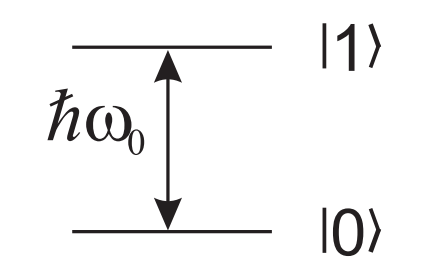
\includegraphics[width=0.15\linewidth]{Figuras/Fig_Harware_NMR_split_Zeeman}
	\caption{Diagrama de energías de una partícula de espín 1/2 en un campo magnético.}
	\label{Fig_Harware_NMR_split_Zeeman}
	\end{figure}


Podemos entender gráficamente la evolución temporal $U = e^{-i \mathcal{H} t/ \hbar}$ bajo el Hamiltoniano de la Ec. (\ref{ec_Hardware_NMR_H_sys_1}) como un movimiento de precesión en la esfera de Bloch al rededor de $\vec{B}_0$, como se muestra en la Fig. \ref{Fig_Harware_NMR_precesion}. Como es habitual, definimos el eje $\hat{z}$ de la esfera de Bloch como el eje de cuantización del Hamiltoniano, con $\ket{0}$ a lo largo de $+\hat{z}$ y $\ket{1}$ a lo largo de $-\hat{z}$.

	\begin{figure}[H]
	\centering 
	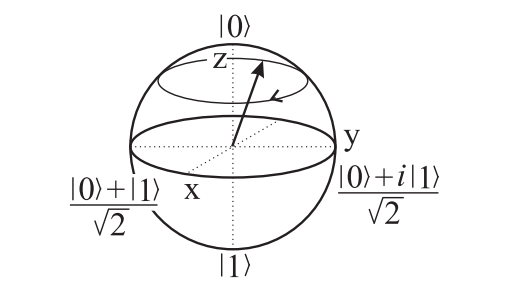
\includegraphics[width=0.45\linewidth]{Figuras/Fig_Harware_NMR_precesion.png}
	\caption{Precesión del valor esperado del espín entorno al campo magnético.}
	\label{Fig_Harware_NMR_precesion}
	\end{figure}

	\begin{mybox_blue}{Esfera de Bloch para el espín}
	Véase que para el espín la representación en la esfera de Bloch no es más que la representación 
	en 3D del vector de espín. 	
	\end{mybox_blue}

	\begin{mybox_blue}{Nota: orientación del espín}
	En las Ecs. (\ref{ec_Hardware_NMR_mu}) y (\ref{ec_Hardware_NMR_gamma}) vemos que el vector de espín
	y el momento dipolar magnético se relacionan por una constate que $\gamma$ que puede ser positiva o 
	negativa, dependiendo del valor de la carga eléctrica de la partícula. Es decir, estos vectores pueden 
	apuntar en la misma dirección o en dirección opuesta. 

	\vspace{0.3cm}	
	Hemos comentado que cuando tenemos un campo magnético, el
	estado de menor energía es aquel con el \textbf{momento dipolar magnético} apuntando en la dirección 
	del campo. Como podemos ver en la Fig. \ref{Fig_Hardware_NMR_espines_en_B}, tenemos dos opciones 
	dependiendo de la carga de la partícula.
		\begin{figure}[H]
		\centering 
		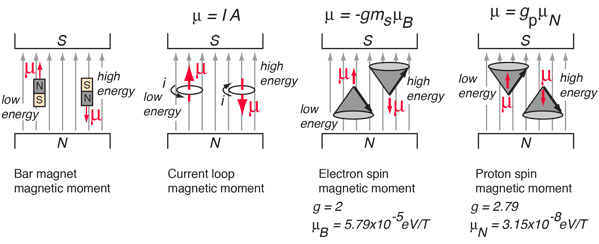
\includegraphics[width=1\linewidth]{Figuras/Fig_Hardware_NMR_espines_en_B.png}
		\caption{Momentos dipolares magnéticos en presencia de un campo magnético externo. En las dos figuras
		de la derecha vemos que, dependiendo de la carga de la partícula, el momento dipolar puede apuntar 
		en la misma dirección o en la contraria al espín. Figura tomada de 
		\url{http://hyperphysics.phy-astr.gsu.edu/hbase/Nuclear/nmr.html}}
		\label{Fig_Hardware_NMR_espines_en_B}
		\end{figure}
	\end{mybox_blue}


Vemos a la demostración de que el valor esperado del espín precesa entorno al campo magnético:

\begin{proof}
\textbf{(Precesión de Larmor, Griffiths \cite{griffiths_schroeter_2018} ejemplo 4.3)} 

Supongamos una partícula con espín 1/2 sometida a un campo magnético en la dirección $\vec{z}$, i.e. $\vec{B}_0 = B_0 \hat{z}$. El Hamiltoniano estará dado por 
	\begin{equation}
	\mathcal{H} = - \gamma B_0 S_z = - \frac{\gamma B_0 \hbar}{2} 
	\begin{bmatrix}	1 & 0 \\ 0 & -1 \end{bmatrix}
	\end{equation}
Los autovectores y autovalores (energías) de este Hamiltoniano son
	\begin{equation}
	\lch 
	\begin{matrix}
	\ket{0} = \begin{bmatrix} 1 \\ 0 \end{bmatrix} \, 
	\text{con energía } E_{\ket{0}} = - (\gamma B_0 \hbar) /2 \, \\
	\ket{1} = \begin{bmatrix} 0 \\ 1 \end{bmatrix} \, 
	\text{con energía } E_{\ket{1}} = + (\gamma B_0 \hbar) / 2
	\end{matrix}
	\right.
	\end{equation}
La energía es menor cando el momento dipolar es paralelo al campo magnético, al igual que en el caso clásico.

Como el Hamiltoniano es independiente del tiempo, la solución general para la ecuación de Schrödinger dependiente de tiempo,
	\begin{equation} \label{ec_Hardware_NMR_schrodinger}
	i \hbar \frac{\partial \ket{\Psi}}{\partial t} = \mathcal{H} \ket{\Psi}
	\end{equation}
puede expresarse en función de estados estacionarios:
	\begin{equation} \label{ec_Hardware_NMR_schrodinger_sol}
	\ket{\Psi (t)} = a  e^{-i E_{\ket{0}} t/ \hbar} \ket{0} + b  e^{-i E_{\ket{1}} t/ \hbar} \ket{1}  =
	\begin{bmatrix}
	a e ^{i \gamma B_0 t/2} \\
	b e ^{i \gamma B_0 t/2}
	\end{bmatrix}
	\end{equation}

Las constantes $a$ y $b$ se pueden determinar mediante las condiciones iniciales:
	\begin{equation}
	\ket{\Psi (t = 0)} = \begin{bmatrix} a \\ b	\end{bmatrix}
	\end{equation}
(por supuesto, $|a|^2 + |b|^2 = 1$). Sin perdida de generalidad, podemos elegir $a = \cos (\alpha/2)$ y $b = \sin (\alpha/2)$, donde $\alpha$ es un ángulo fijo cuyo significado físico veremos dentro de poco.
Tenemos entonces
	\begin{equation}
	\ket{\Psi (t)} = 
	\begin{bmatrix} 
	\cos (\alpha/2) e^{i \gamma B_0 t/2} \\ 
	\sin (\alpha/2) e^{-i \gamma B_0 t/2} 
	\end{bmatrix}
	\end{equation}
Para ver que está pasando con el espín bajo la evolución de este Hamiltoniano, calculemos el calor esperado del espín $\vec{S}$ como función del tiempo.
	\begin{align}
	\left\langle S_x \right\rangle = & \, \bra{\Psi(t)} S_x \ket{\Psi(t)} = 
	\nonumber \\
	= & \, \Lc \psi_0^* \quad \psi_1^* \Rc 
	\begin{bmatrix} 1 & 0 \\ 0 & 1 \end{bmatrix}  
	\begin{bmatrix} \psi_0 \\ \psi_1 \end{bmatrix} 
	\nonumber \\
	= & \, \Lc a e ^{-i \gamma B_0 t/2} \qquad  b e ^{-i \gamma B_0 t/2} \Rc 
	\frac{\hbar}{2} \begin{bmatrix} 0 & 1 \\ 1 & 0 \end{bmatrix} 
	\begin{bmatrix} \cos (\alpha/2) e^{i \gamma B_0 t/2} \\	\sin (\alpha/2) e^{-i \gamma B_0 t/2} \end{bmatrix} 
	\nonumber \\
	= & \, \frac{\hbar}{2} \sin \alpha \cos (\gamma B_0 t ) 
	\end{align}
De forma análoga,
	\begin{align}
	\left\langle S_y \right\rangle = & \, - \frac{\hbar}{2} \sin \alpha \sin (\gamma B_0 t )  \\
	\left\langle S_z \right\rangle = & \frac{\hbar}{2} \cos \alpha
	\end{align}

Con lo cual, $\left\langle \vec{S} \right\rangle$ está inclinado un ángulo $\alpha$ respecto al eje $\hat{z}$, y precesa al rededor del campo con una frecuencia 
	\begin{equation}
	f_0 = \omega_0 / 2 \pi = \gamma B_0 / 2 \pi
	\end{equation}
(la frecuencia de Larmor) al igual que en el caso clásico (una peonza inclinada). No tenemos ninguna sorpresa aquí, pues el teorema de Ehrenfest nos asegura que los valores esperados evolucionan de acuerdo a las leyes clásicas del movimiento\footnote{Algunos autores limitan esta afirmación solo al par de ecuaciones $\left\langle p \right\rangle = m d \left\langle x \right\rangle / dt$ y $\left\langle - \partial V / \partial x \right\rangle = d \left\langle p \right\rangle / dt$.} (puede verse esto en el Griffiths, \cite{griffiths_schroeter_2018}). 
	\begin{figure}[H]
	\centering 
	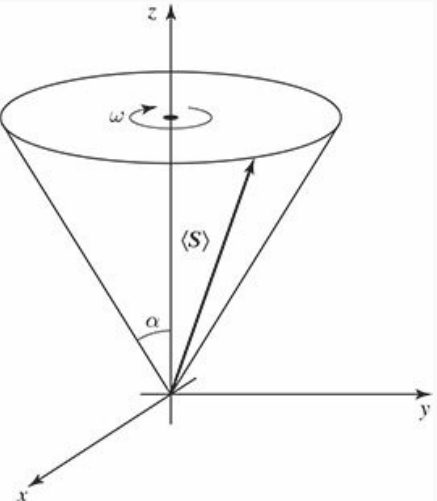
\includegraphics[width=0.30\linewidth]{Figuras/Fig_Harware_NMR_precession_griffiths}
	\caption{Precesión de Larmor en un campo magnético uniforme.}
	\label{Fig_Harware_NMR_precession_griffiths}
	\end{figure}

\end{proof}


	\Ejercicio{Verifica que la Ec. (\ref{ec_Hardware_NMR_schrodinger_sol}) es solución de la ecuación de Schrödinger, Ec. (\ref{ec_Hardware_NMR_schrodinger})}

El Hamiltoniano de espín para una molécula con $n$ núcleos desacoplados viene dado por 
	\begin{equation} \label{ec_Hardware_NMR_H_single}
	\mathcal{H}_0 = - \sum_{i=1}^n  \omega_0^i S_z^i
	\end{equation}
Véase que, los espines de especies nucleares diferentes (espines heteronucleares) tendrán diferentes valores de $\omega_0^i$, así como también es posibles que los espines de la misma especie nuclear (espines homonucleares) que formen una molécula  tengan también diferentes valores de esta frecuencia.


			\SubsubiIt{Espines que interactúan.} 

Para espines nucleares en moléculas, la naturaleza nos proporciona dos mecanismos de interacción diferentes que vamos a describir: 
\begin{itemize}
	\item \textbf{Interacción directa dipolo-dipolo.}
	
La interacción magnética dipolo-dipolo es similar a la interacción entre dos barras magnéticas cercanas. Tiene lugar puramente a través del espacio (no se requiere ningún medio para esta interacción) y depende del vector internuclear $\vec{r}_{ij}$ que conecta los dos núcleos $i$ y $j$, tal y como describe el Hamiltoniano
	\begin{equation} \label{ec_Hardware_NMR_H_dipolo-dipolo}
	\mathcal{H}_D = \sum_{i<j} \frac{\mu_0 \gamma_i \gamma_j}{4 \pi | \vec{r}_{ij}|^3 \hbar} 
	\lc \vec{S}^i \cdot \vec{S}^j - \frac{3}{| \vec{r}_{ij}|^2} \lp \vec{S}^i \cdot \vec{r}_{ij} \rp \lp \vec{S}^j \cdot \vec{r}_{ij} \rp \rc
	\end{equation}
donde $\mu_0$ es la permeabilidad magnética habitual del espacio libre. 

No vamos a entrar en dalles sobre esta interacción, pues usualmente se promedia y no tiene efecto.
	
	\item \textbf{Interacción del contrato de Fermi mediada por electrones (acoplamiento J).}

	El segundo mecanismo de interacción entre los espines nucleares de una molécula es el acoplamiento $J$ o acoplamiento escalar. Esta interacción está mediada por los electrones compartidos en los enlaces químicos entre los átomos, y es debido al solapamiento de la función de onda del electrón compartido con los dos núcleos acoplados. Es decir, una interacción de contacto de Fermi. La fuerza de acoplamiento de enlace J depende de la especie nuclear respectiva y disminuye con el número de enlaces químicos que separan los núcleos.

El Hamiltoniano es
	\begin{equation}
	\mathcal{H} = \frac{1}{\hbar} \sum_{i <j} 2 \pi J_{ij} S^i S^j = 
	\frac{1}{\hbar} \sum_{i < j} 2 \pi J_{ij} \lp S_x^i S_x^j + S_y^i S_y^j + S_z^i S_z^j  \rp
	\end{equation}
donde $J_{ij}$ es la fuerza de acoplamiento entre los espines $i$ y $j$. Cuando $| \omega_0^i - \omega_0^j |$ es mucho más grande que el acoplamiento $J_{ij}$ ($| \omega_0^i - \omega_0^j | \gg 2 \pi |J_{ij}|$), los acoplamiento transversos se pueden despreciar. De esta forma, el Hamiltoniano se simplifica
	\begin{equation} \label{ec_Hardware_NMR_J_coupling}
	\boxed{\mathcal{H}_j = \frac{1}{\hbar} \sum_{i < j}^n 2 \pi J_{ij} S_z^{i} S_z^{j}}
	\end{equation}
Esta condición ($| \omega_0^i - \omega_0^j | \gg 2 \pi |J_{ij}|$) se cumple fácilmente para los espines heteronucleares y que también puede cumplirse para las moléculas homonucleares pequeñas.

La interpretación del término de acoplamiento escalar de la Ec. (\ref{ec_Hardware_NMR_J_coupling})\textit{ es que un espín ``siente'' un campo magnético estático a lo largo de $\pm z$ producido por los espines vecinos}, además del campo $\vec{B}_0$ aplicado externamente. Este campo adicional desplaza los niveles de energía como podemos ver en la Fig. \ref{Fig_Harware_NMR_diagrama}. Como resultado, la frecuencia de Larmor del espín $i$ se mueve en una cantidad $-J_{ij}/2$ si el espín $j$ está en el estado $\ket{0}$ (lineas rojas) y una cantidad $+J_{ij}/2$ si está en el estado $\ket{1}$ (líneas azules).  

	\begin{figure}[H]
	\centering 
	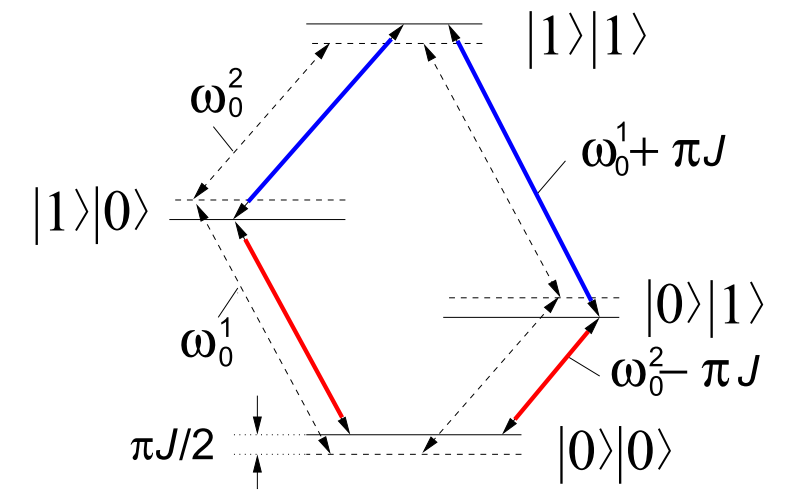
\includegraphics[width=0.4\linewidth]{Figuras/Fig_Harware_NMR_diagrama}
	\caption{Diagrama de niveles de energía para dos espines desacoplados (líneas discontinuas) 
	y dos espines acoplados (líneas continuas) por un Hamiltoniano de la forma de la Ec.
	(\ref{ec_Hardware_NMR_J_coupling}) (en unidades de $\hbar$). Marcadas en rojo están las dos transiciones en las que el espín que no cambia está en el estado $\ket{0}$, mientras que en azul están en las que el espín que no cambia está en el estado $\ket{1}$. Vemos que la energía de transición de las primera disminuye, mientras que de las segundas aumenta.}
	\label{Fig_Harware_NMR_diagrama}
	\end{figure}

\end{itemize}

			\SubsubiIt{Hamiltoniano completo.}

En resumen, la forma más simple del Hamiltoniano para un sistema de $n$ espines nucleares acoplados es, pues (de las Ecs. (\ref{ec_Hardware_NMR_H_single}) y (\ref{ec_Hardware_NMR_J_coupling}))
	\begin{equation} \label{ec_Hardware_NMR_H_sys_final}
	\boxed{\mathcal{H}_{sys} = - \sum_{i}^n \omega_0^i S_z^{i}  + \frac{1}{\hbar} \sum_{i<j} 2 \pi J_{ij} S_z^i S_z^j}
	\end{equation}
	

		\subsection{Hamiltoniano de control} \label{sec_subsub_Harware_NMR_H_control}

			\SubsubiIt{Campos de radiofrecuencia}

Pasemos ahora a los mecanismos físicos para controlar el sistema de RMN. El estado de una partícula de espín $1/2$ en un campo magnético estático $\vec{B}_0$ a lo largo del eje $\hat{z}$ puede manipularse aplicando un campo electromagnético $\vec{B}_1(t)$ que gira en el plano $\hat{x}-\hat{y}$ a frecuencia $\omega_{rf}$, en o cerca de la frecuencia de precesión del espín $\omega_0$. El Hamiltoniano de espín  correspondiente al campo de radiofrecuencia (RF) es, análogo a la Ec. (\ref{ec_Hardware_NMR_H_sys_1}) para el campo estático $B_0$,
	\begin{equation} 
	\mathcal{H}_{rf} = - \gamma B_1 \Lc \cos (\omega_{rf} + \phi) S_x + \sin (\omega_{rf} + \phi) S_y \Rc \,
	\end{equation}
donde $\phi$ es la fase del campo de RF, y $B_1$ su amplitud. Para $n$ espines tenemos
	\begin{equation} \label{ec_Hardware_NMR_H_rf}
	\boxed{\mathcal{H}_{rf} = - \sum_{i}^n \gamma_i B_1 \Lc \cos (\omega_{rf} t + \phi) S_x^i + \sin (\omega_{rf} t+ \phi ) S_y^i \Rc} \, ,
	\end{equation}
	
	\begin{mybox_blue}{Nota: implementación de un campo rotante en el laboratorio}
	En la práctica, se aplica un campo magnético que oscila a lo largo de un eje fijo en el
	laboratorio, perpendicular al campo magnético estático. Este campo oscilante puede
	descomponerse en dos campos contrarrotatorios, uno de los cuales gira a $\omega_{rf}$ en la
	misma dirección que el espín y, por tanto, puede establecerse en resonancia con el espín o
	cerca de ella. La  otra componente gira en la dirección opuesta y, por lo tanto, está muy 
	lejos de la resonancia (en aproximadamente $2\omega_0$). Como veremos, su único efecto es un
	desplazamiento insignificante de la frecuencia de Larmor, llamado desplazamiento Bloch-Siegert.
	\end{mybox_blue}

			\SubsubiIt{Sistema de referencia rotante (\textit{rotating frame}).} 
			
El movimiento de un espín nuclear individual sometido a un campo magnético estático y giratorio es bastante complejo cuando se describe en el sistema de coordenadas habitual del laboratorio (el marco del laboratorio). Sin embargo, se simplifica mucho describiendo el movimiento en un \textbf{sistema de coordenadas que gira} alrededor de $\hat{z}$ a frecuencia $\omega_{rf}$ (el \textbf{rotating frame}):
	\begin{equation} \label{ec_Hardware_NMR_psi_rot}
	\ket{\psi}^{rot} = \exp \lp -i \omega_{rf} t S_z/\hbar \rp \ket{\psi}
	\end{equation}
Para un solo espín libre, el Hamiltoniano será la suma (\ref{ec_Hardware_NMR_H_single}) y (\ref{ec_Hardware_NMR_H_rf}) (con $n=1$), es decir,
	\begin{equation} \label{ec_Hardware_NMR_H_lab_single}
	\mathcal{H} = - \omega_0 S_z - \omega_1 \Lc \cos (\omega_{rf} t+ \phi) S_x + \sin (\omega_{rf} t + \phi) S_y \Rc
	\end{equation}
Este Hamiltoniano junto con el estado en el sistema de referencia estático cumplen la ecuación de Schrödinger
	\begin{equation}
	i \hbar \frac{d \ket{\psi}}{dt} = \mathcal{H} \ket{\psi}
	\end{equation}
Sustituyendo el cambio de variable de la Ec. (\ref{ec_Hardware_NMR_H_sys_final}) en la ecuación de Schrödinger, podemos calcular como tendría que ser el $\mathcal{H}^{rot}$ que cumpla
	\begin{equation}
	i \hbar \frac{d \ket{\psi}^{rot}}{dt} = \mathcal{H}^{rot} \ket{\psi}^{rot}
	\end{equation}
Puede ver que el resultado es
	\begin{equation} \label{ec_Hardware_NMR_H_rot_single}
	\boxed{\mathcal{H}^{rot} = - (\omega_0 - \omega_{rf}) S_z - \omega_1 \Lc \cos (\phi) S_x + \sin  (\phi) S_y \Rc}
	\end{equation}

%\Ejercicio{Haz el cambio de variable comentado y calcula $\mathcal{H}^{rot}$ de la Ec. (\ref{ec_Hardware_NMR_H_rot_single})}

Naturalmente, el campo de RF se encuentra a lo largo de un eje fijo en el sistema de referencia que gira a $\omega_{rf}$. El movimiento del espín visto desde un sistema de referencia o el otro es diferente. 
\begin{itemize}
	\item En el \textbf{sistema laboratorio (en reposo)}, al aplicar el campo magnético rotante $\vec{B}_1$ lo que sucede es que \textit{el valor esperado del espín rota en espiral, bajando por la esfera}, como podemos ver en la Fig. \ref{Fig_Harware_NMR_espiral_bloch}b. 

	\begin{figure}[t]
	\centering 
	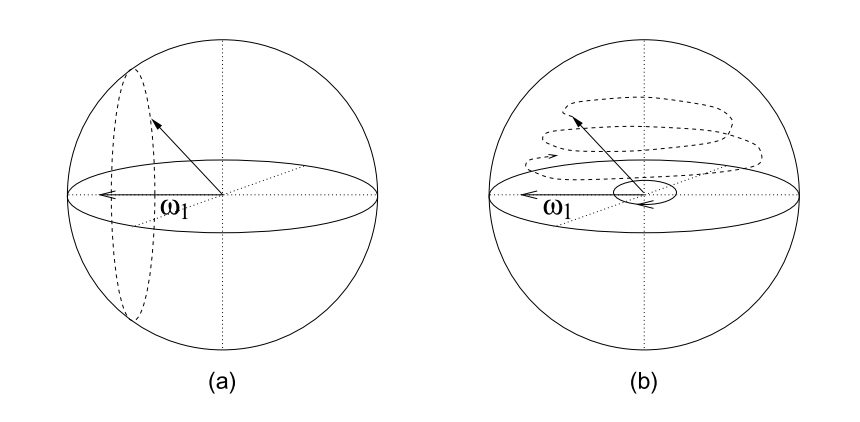
\includegraphics[width=0.55\linewidth]{Figuras/Fig_Harware_NMR_espiral_bloch}
	\caption{Nutación de un espín sometido a un campo de RF transversal observada en el marco de rotación (a) y observada en el marco de laboratorio (b).}
	\label{Fig_Harware_NMR_espiral_bloch}
	\end{figure}

	
	\item En el \textbf{sistema rotante}, tenemos dos casos:
	
	\begin{itemize}
		\item Caso \textbf{resonante} ($\omega_{rf} = \omega_0$): en este caso el primer término de la Ec. (\ref{ec_Hardware_NMR_H_rot_single}) desaparece. En este caso, un observador en el sistema rotante verá el espín simplemente \textit{precesar} alrededor de $\vec{B}_1$ (Fig. \ref{Fig_Harware_NMR_espiral_bloch}a), un movimiento llamado nutación. La elección de $\phi$ controla el eje de nutación.
		
		
		
		\item Caso \textbf{fuera de resonancia}: Si el campo de RF está fuera de resonancia con respecto a la frecuencia de espín en $\Delta \omega = \omega_0 - \omega_{rf}$, el espín precesa en el marco de rotación alrededor de un eje inclinado con respecto al eje $\vec{z}$ en un ángulo
	\begin{equation}
	\alpha = \arctan (\omega_1 / \Delta \omega)
	\end{equation}
como se ilustra en la Fig. \ref{Fig_Harware_NMR_nutacion_inclinada}.

	\begin{figure}[H]
	\centering 
	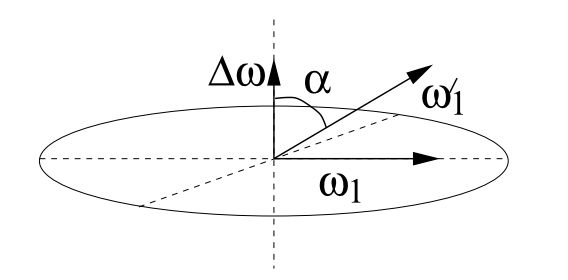
\includegraphics[width=0.35\linewidth]{Figuras/Fig_Harware_NMR_nutacion_inclinada}
	\caption{Eje de rotación (en el marco giratorio) durante un pulso de radiofrecuencia fuera de resonancia.}
	\label{Fig_Harware_NMR_nutacion_inclinada}
	\end{figure}
	
	\end{itemize}		

\end{itemize}

En este último caso se deduce que \textbf{el campo de RF no tiene prácticamente ningún efecto sobre espines que están lejos de la resonancia}, ya que $\alpha$ es muy pequeño cuando $|\Delta \omega | \gg \omega_1$ (ver Fig. \ref{Fig_Harware_NMR_espiral_bloch_2}). Si todos los espines tienen frecuencias de Larmor bien separadas, en principio podemos \textbf{rotar selectivamente} cualquier qúbit sin rotar los otros espines.



Los pulsos moderadamente fuera de resonancia ($|\Delta \omega| \approx \omega_1$) hacen girar el espín, pero debido a la inclinación del eje de rotación, un solo pulso de este tipo no puede, por ejemplo, voltear un espín de $|0 \rangle$ a $|1 \rangle$ (véase de nuevo la Fig. \ref{Fig_Harware_NMR_espiral_bloch_2}). Por supuesto, los pulsos fuera de resonancia también pueden ser útiles, por ejemplo para la implementación directa de rotaciones sobre un eje fuera del plano $\hat{x} - \hat{y}$.

	\begin{figure}[H]
	\centering 
	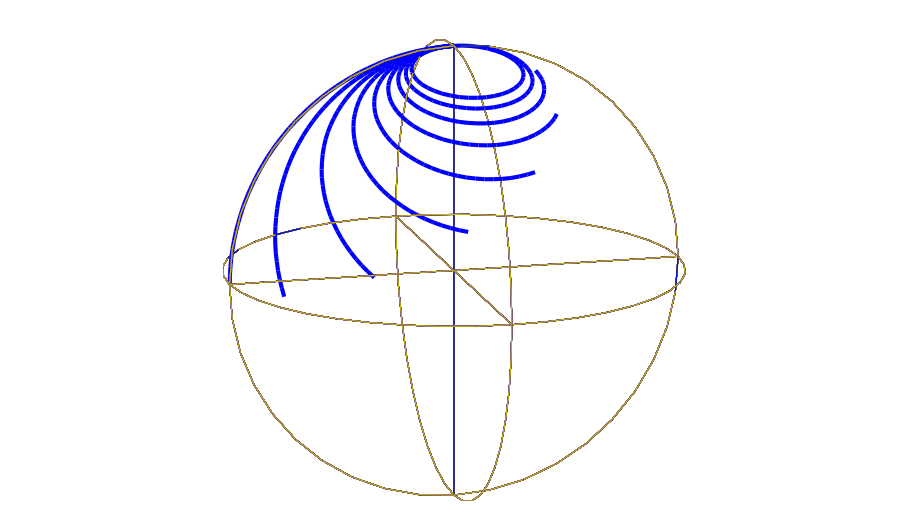
\includegraphics[width=0.4\linewidth]{Figuras/Fig_Harware_NMR_espiral_bloch_2.png}
	\caption{Trayectoria en la esfera de Bloch (en el sistema de referencia rotante) descrita por un qubit inicialmente en $\ket{0}$ (a lo largo de $+\hat{z}$), después de aplicar un pulso de 250 $\mu s$ de intensidad $\omega_1 = 1$ kHz fuera de resonancia en $0$, $0.5$, $1$, $\dots$ 4 kHz. En resonancia, el pulso produce una rotación $90º$. Lejos de la resonancia, el qúbit apenas rota alejándose de $\ket{0}$.}
	\label{Fig_Harware_NMR_espiral_bloch_2}
	\end{figure}

Por otro lado, podemos elegir trabajar en \textbf{un sistema de referencia que rote a} $\bm \omega_0$ (en vez de a $\omega_{rf}$, donde
	\begin{equation}
	\boxed{\mathcal{H}^{rot} = - \omega_1 \Lc \cos ((\omega_{rf} - \omega_0)t + \phi) S_x + \sin ((\omega_{rf} - \omega_0)t + \phi) S_y \Rc}
	\end{equation}

Esta transformación no da un Hamiltoniano de RF independiente del tiempo (a menos que $\omega_{rf} = \omega_0$), como fue el caso para $\mathcal{H}^{rot}$ en la Ec. \ref{ec_Hardware_NMR_H_rot_single}). Sin embargo, es un punto de partida natural para la extensión al caso de \textbf{múltiples espines}, donde puede introducirse un marco de rotación separado para cada espín:
	\begin{equation} \label{ec_Hardware_NMR_psi_rot_multi}
	\ket{\psi}^{rot} = \Lc \prod_i \exp (-i \omega_0^i t S^i_z/\hbar ) \Rc \ket{\psi}
	\end{equation}
En presencia de múltiples campos de RF indexados con $r$, el Hamiltoniano en este marco de referencia rotante e $\omega_0$ nos queda
	\begin{equation}
	\boxed{\mathcal{H}^{rot} = \sum_{i,r} - \omega_1^r \Lc \cos ((\omega_{rf}^r - \omega_0^i)t + \phi^r) S_x^i + \sin ((\omega_{rf}^r - \omega_0^i) t +\phi^r) S_y^i  \Rc}
	\end{equation}
donde las amplitudes $\omega_i^r$ y las fases $\phi^r$ están bajo control. 

El Hamiltoniano del sistema de la Ec. (\ref{ec_Hardware_NMR_H_sys_final}) se simplifica en el sistema de referencia multi-rotante de la Ec. (\ref{ec_Hardware_NMR_psi_rot_multi}): el termino $S_z^i$ desparece dejando solo el término de acoplamiento $J_{ij} S_z^i S_z^j$, que permanecen invariantes.

En resumen, en el sistema de referencia multi-rotante, el Hamiltoniano de $NMR$ $\mathcal{H} = \mathcal{H}_{sys} + \mathcal{H}_{control}$ toma la forma
	\begin{align} 
	& ~~~~ \boxed{ \mathcal{H}_{sys} =  \, \frac{1}{\hbar} \sum_{i<j} 2 \pi J_{ij} S_z^i S_z^j} \label{ec_Hardware_NMR_H_sys_final_multi_rot} \\
	&\boxed{\mathcal{H}_{control} =  \, \sum_{i,j} - \omega_1^r \Lc \cos ((\omega_{rf}^r - \omega_0^i)t +\phi^r) S_x^i + \sin ((\omega_{rf}^r-\omega_0^i)t +\phi^r) S^i_y \Rc} \label{ec_Hardware_NMR_H_control_final_multi_rot}
	\end{align}








	\section{Técnicas de pulsos elementales.} \label{sec_sub_Harware_NMR_pulsos} 

Esta sección inicia nuestra discusión del tema principal de este artículo, una revisión de las \textbf{técnicas de control} desarrolladas en la computación cuántica de RMN para sistemas cuánticos acoplados de dos niveles. Comenzamos con una rápida visión general del lenguaje de los circuitos cuánticos y sus importantes teoremas de universalidad, luego lo conectamos con el lenguaje de las secuencias de pulsos tal y como se utiliza en la RMN, e indicamos cómo se pueden simplificar las secuencias de pulsos. Las principales aproximaciones empleadas en esta sección son que los pulsos pueden ser \textbf{fuertes} comparados con el Hamiltoniano del sistema mientras se dirigen selectivamente a \textbf{un solo qúbit} a la vez, y pueden ser perfectamente implementados. 

		\subsection{Control cuántico, circuitos y pulsos}

El objetivo del control cuántico, en el contexto de la computación cuántica, es la implementación de una \textbf{transformación unitaria} $U$, especificada en términos de una secuencia $U = U_k U_{k-1} \dots U_2 U_1$ de puertas cuánticas estándar $U_i$, que actúan localmente (normalmente sobre uno o dos qubits) y son sencillas de implementar. Como es habitual en las operaciones unitarias, las $U_i$ se ordenan en el tiempo de derecha a izquierda.

			\SubsubiIt{Puertas cuánticas y circuitos}

La rotación básica de un qúbit simple son las rotaciones de la forma (\ref{ec_puertas_simples_Rn}), es decir
$$
R_{\hat{n}} (\theta) = \exp \lc - \frac{i \theta \hat{n} \cdot \vec{\sigma}}{2} \rc
$$

Como ya hemos comentado en la sección \ref{sec_subsub_puertas_euler}, usando la \textbf{parametrización de Euler}  podemos general cualquier rotación sobre la esfera de Bloch usando tres rotaciones sobre dos ejes (Ec. (\ref{ec_puertas_simples_rotacion_1})). En esa sección elegimos las rotaciones en $\hat{z}$ y $\hat{y}$, pero en esta vamos a usar las siguientes:
	\begin{equation}
	U = e^{i \alpha} R_x(\beta) R_y (\gamma) R_x (\delta)
	\end{equation}

Como también comentamos, la puerta básica de dos qúbits es la CNOT (Ec. (\ref{ec_multiqubit_CNOT})). 

Un teorema básico de la computación cuántica es que salvo una fase global irrelevante, cualquier $U$ que actúe sobre $n$ qubits puede componerse a partir de puertas $U_{CNOT}$ y $R_{\hat{n}}(\theta)$ \cite{nielsen_chuang_2010} . Así, el problema del control cuántico puede reducirse a la implementación de $U_{CNOT}$ y rotaciones de qúbits simples, donde se requieren al menos dos rotaciones no triviales (veremos esto en detalle en la sección \ref{sec_elementos_universalidad}). Se conocen otros conjuntos de puertas universales de este tipo, pero éste es el que se ha empleado en la RMN.


			\SubsubiIt{Implementación de puertas de un qúbit.}

Las rotaciones en qúbits individuales pueden implementarse directamente en el sistema de referencia rotante utilizando pulsos de RF. Del Hamiltoniano de control, Ec. (\ref{ec_Hardware_NMR_H_sys_final_multi_rot}), se deduce que cuando se aplica un campo de RF de amplitud $\omega_1$ a un sistema de un único espín con $\omega_{rf} = \omega_0$, el espín evoluciona bajo la transformación
	\begin{equation} \label{ec_Hardware_NMR_U_arbitrario}
	U = e^{i \frac{\mathcal{H}_{control}}{\hbar}} = \exp \Lc i \omega_1 \lp  \cos \phi S_x + \sin \phi S_y \rp \frac{t_{p \omega}}{\hbar} \Rc
	\end{equation}
donde $t_{p \omega}$ es la \textbf{anchura del pulso} (o longitud), la duración temporal del pulso de RF. $U$ describe una rotación en la esfera de Bloch de un ángulo $\theta$ proporcional al producto de $t_{p\omega}$ y $\omega_1 = \gamma B_1$, y al rededor de un eje en el plano $\hat{x}-\hat{y}$ determinado por una fase $\phi$.

\begin{itemize}
	\item Así, un pulso con fase $\phi = \pi$ y $\omega_1 t_{p\omega} = \pi/2$ realizará $R_x(90)$ (ver Ec. (\ref{ec_puertas_simples_Rn})), que es una rotación $90$º sobre $\hat{x}$, denotada para abreviar como $\sqrt{X}$.
	\item Un pulso similar pero dos veces más largo realiza una rotación $R_x(180) =  X$.
	\item Cambiando la fase del pulso RF a $\phi = -\pi/2$, pueden implementarse de forma similar $\sqrt{Y}$ e $Y$
	\item Para $\phi = 0$ y $\omega_1 t_{p\omega} = \pi/2$, se obtiene una rotación negativa alrededor de $\hat{x}$: $R_x (-90) = \sqrt{X^\dagger}$.
	\item De forma similar $\phi = \pi/2$ y $\omega_1 t_{p\omega} = \pi/2$ da $\sqrt{Y^\dagger}$.
\end{itemize}
Para sistemas multiqubit, se utilizan subíndices para indicar sobre qué qúbit actúa la operación, por ejemplo, $Z^\dagger_3$ es una rotación de $180$º del qúbit 3 alrededor de $- \hat{z}$.

Por tanto, no es necesario aplicar el campo de RF a lo largo de diferentes ejes espaciales en el marco del laboratorio para realizar rotaciones $\hat{x}$ y $\hat{y}$. Más bien, la fase del campo de RF determina el eje de nutación en el marco de rotación. Además, nótese que sólo importa la fase relativa entre pulsos aplicados al mismo espín. La fase absoluta del primer impulso en un espín determinado no tiene importancia en sí misma. Sólo establece una referencia de fase con la que deben compararse las fases de todos los pulsos posteriores en ese mismo espín, así como la lectura de ese espín.

Anteriormente señalamos que la capacidad de implementar rotaciones arbitrarias sobre $\ket{x}$ y $\ket{y}$ es suficiente para realizar rotaciones arbitrarias de un solo qúbit (Ec. \ref{ec_Hardware_NMR_U_arbitrario}). Dado que las rotaciones $\hat{z}$ son muy comunes, existen dos descomposiciones explícitas útiles de $R_z(\theta)$ en términos de las rotaciones $\hat{x}$ y $\hat{y}$:
	\begin{equation}
	R_z (\theta) = \sqrt{X} R_y (\theta) \sqrt{X^\dagger} = \sqrt{Y} R_x(-\theta) \sqrt{Y^\dagger}
	\end{equation}


			\SubsubiIt{Implementación de puertas a dos qúbits} 

La puerta de dos qúbits más natural es la generada directamente por el Hamiltoniano de acoplamiento espín-espín. Para espines nucleares en una molécula en solución líquida, el Hamiltoniano de acoplamiento viene dado por la Ec. (\ref{ec_Hardware_NMR_J_coupling})  (tanto en el sistema  laboratorio como en el sistema de rotación), a partir de la cual obtenemos el operador de evolución temporal $U_J(t) = \exp \lc - i 2\pi J S_z^1 S_z^2 t /\hbar^2 \rc$, o en forma matricial
	\begin{equation} \label{ec_Hardware_NMR_UJ}
	U_J (t) = 
	\begin{bmatrix}
	e^{-i \pi Jt/2} & 0 & 0 & 0 \\
	0 & e^{+i \pi Jt/2} & 0 & 0 \\
	0 & 0 & e^{+i \pi Jt/2} & 0 \\
	0 & 0 & 0 & e^{-i \pi Jt/2}
	\end{bmatrix}
	\end{equation}
Si se permite que esta evolución ocurra durante un tiempo $t = 1/2J$ se obtiene una transformación conocida como \textbf{puerta de fase controlada}, salvo un desplazamiento de fase de 90º en cada qúbit y una fase global (y por tanto irrelevante):
	\begin{equation}
	U_{CPHASE} = \sqrt{-i} \sqrt{Z^\dagger_1} \sqrt{Z^\dagger_2} U_J (1/2J) = 
	\begin{bmatrix}
	1 & 0 & 0  & 0 \\
	0 & 1 & 0  & 0 \\
	0 & 0 & 1 & 0 \\
	0 & 0 & 0  & -1 
	\end{bmatrix}	 
	\end{equation}
Esta puerta es equivalente a la conocida puerta CNOT salvo un cambio de base del qúbit objetivo y un desplazamiento de fase en el qúbit de control:
	\begin{align} \label{ec_Hardware_NMR_implementacion_CNOT}
	U_{CNOT} = & \, i Z_1 \sqrt{Y^\dagger_2} U_{CPHASE} \sqrt{Y_2} \nonumber \\
	= & \, i Z_1 \sqrt{Y^\dagger_2} \Lc \sqrt{-i} \sqrt{Z^\dagger_1} \sqrt{Z^\dagger_2} U_J (1/2J)  \Rc \sqrt{Y_2} \nonumber \\
	= & \, \sqrt{i} \sqrt{Z_1} \sqrt{Z_2^\dagger} \sqrt{X_2} U_j (1/2J) \sqrt{Y_2}  \nonumber \\
	= & \, 
	\begin{bmatrix}
	1 & 0 & 0  & 0 \\
	0 & 1 & 0  & 0 \\
	0 & 0 & 0 & 1 \\
	0 & 0 & 1  & 0 
	\end{bmatrix}
	\end{align}

El núcleo de esta secuencia, $\sqrt{X_2} U_j (1/2J) \sqrt{Y_2}$, puede entenderse gráficamente mediante la Fig. \ref{Fig_Harware_NMR_implementacion_CNOT}, suponiendo que los espines comienzan a lo largo de $\pm \hat{z}$. Primero, un pulso en el espín 2 que lo rota de $\hat{z}$ a $\hat{y}$. A continuación, se deja que el sistema de espín evolucione libremente durante $1/2J_{12}$ segundos. Como \textbf{la frecuencia de precesión del espín 2 se desplaza $\pm J_{12}/2$ dependiendo de si el espín 1 está en $\ket{1}$ o $\ket{0}$} (ver Fig. \ref{Fig_Harware_NMR_diagrama}), el espín 2 llegará en $1/2J_{12}$ segundos a $+\hat{y}$ o $- \hat{y}$, dependiendo del estado del espín 1. Finalmente, un pulso de 90º sobre el espín 2 alrededor del eje $\hat{x}$ hace girar el espín 2 de nuevo a $+\hat{z}$ si el espín 1 está en $\ket {0}$, o a $-\hat{z}$ si el espín 1 está en $\ket{1}$.

	\begin{figure}[H]
	\centering 
	\includegraphics[width=0.7\linewidth]{Figuras/Fig_Harware_NMR_implementacion_CNOT}
	\caption{Representación en esfera de Bloch del funcionamiento de la puerta CNOT$_{12}$ entre dos qubits 1 y 2 acoplados por $2 \pi J S_z^1S_z^2/\hbar$ . Aquí se reprensenta el estado del qúbit 2 (el qúbit objetivo de la CNOT), que comienza en $\ket{0}$ (a lo largo de $\hat{z}$) y se representa en un marco de referencia que gira alrededor de $\hat{z}$ a $\omega_0^2/2 \pi$. Las flechas continuas y discontinuas corresponden al caso en que el qúibit 1 (de controlo) está en $\ket{0}$ y $\ket{1}$ respectivamente. Figura tomada de \cite{NMR_hardware}.}
	\label{Fig_Harware_NMR_implementacion_CNOT}
	\end{figure}

	\Ejercicio{Vamos a verificar el paso de la esfera 2 a la 3 de la Fig. \ref{Fig_Harware_NMR_implementacion_CNOT}. Multiplica la matriz de la Ec. (\ref{ec_Hardware_NMR_UJ}) por los dos estados de la segunda esfera de la Fig. \ref{Fig_Harware_NMR_implementacion_CNOT}. Toma $t=1/2J$ y escribe los estados resultantes de la forma \ref{ec_qubit_caso_general} (recuerda que las fases globales no son importantes)}


El resultado neto es que el espín 2 se invierte si y sólo si el espín 1 está en $\ket{1}$, lo que corresponde exactamente a la tabla de verdad clásica para la CNOT. Las rotaciones $\hat{z}$ adicionales de la Ec. (\ref{ec_Hardware_NMR_implementacion_CNOT}) son necesarias para dar a todos los elementos de $U_{CNOT}$ la misma fase, por lo que la secuencia también funciona para estados de entrada en superposición.

Si el Hamiltoniano de interacción espín-espín no es de la forma $S_z^i S_z^j$ sino que contiene también componentes transversales (como en las Ec. (\ref{ec_Hardware_NMR_H_dipolo-dipolo})), se necesitan otras secuencias de pulsos más complicadas para realizar las puertas CPHASE y CNOT.

Si dos espines no están directamente acoplados entre sí, todavía es posible realizar una puerta CNOT entre ellos, siempre y cuando exista una red de acoplamientos que conecte los dos qúbits. Por ejemplo, supongamos que queremos realizar una puerta CNOT con el qúbit 1 como control y el qúbit 3 como objetivo, CNOT$_{13}$, pero 1 y 3 no están acoplados entre sí. Si ambos están acoplados al qúbit 2, como en la red de acoplamiento de la Fig. \ref{Fig_Harware_NMR_posible_couplings}b, podemos primero intercambiar el estado de los qúbits 1 y 2 (mediante la secuencia CNOT$_{12}$ CNOT$_{21}$ CNOT$_{12}$, es decir, una puerta SWAP como la de la Fig. \ref{Fig_elementos_Equiv_CNOTs}), luego realizar un CNOT$_{23}$, y finalmente intercambiar de nuevo los qubits 1 y 2. El efecto neto es CNOT$_{13}$. Por extensión, se requieren como máximo $O(n)$ operaciones de intercambio para realizar una CNOT entre cualquier par de qúbits en una cadena de $n$ espines con sólo acoplamientos de vecino más cercano (Fig. \ref{Fig_Harware_NMR_posible_couplings}b). Las operaciones SWAP también se pueden utilizar para realizar puertas de dos qúbits entre dos qúbits cualesquiera que estén acoplados a un qúbit ``bus'' común (Fig. \ref{Fig_Harware_NMR_posible_couplings}c).

Por el contrario, si un qúbit está acoplado a muchos otros qúbits (Fig. \ref{Fig_Harware_NMR_posible_couplings}a) y queremos realizar una CNOT entre sólo dos de ellos, debemos \textbf{eliminar el efecto de los acoplamientos restantes}. Esto se puede lograr utilizando la técnica de \textbf{reenfoque}, que ha sido ampliamente adoptada en una variedad de experimentos de RMN.


	\begin{figure}[H]
	\centering 
	\includegraphics[width=0.65\linewidth]{Figuras/Fig_Harware_NMR_posible_couplings.png}
	\caption{Tres posibles redes de acoplamiento entre cinco qúbits. (a) Una red de acoplamiento completa. En la práctica, estas redes siempre tendrán un tamaño limitado, ya que las interacciones físicas tienden a disminuir con la distancia. (b) Una red de acoplamiento de vecino más próximo. Este tipo de cadenas lineales con acoplamientos de vecino más próximo, o variantes bidimensionales, se utilizan en muchas propuestas de estado sólido. (c) Acoplamiento a través de un ``bu''. Es el caso, por ejemplo, de los esquemas de trampas de iones. Al igual que en el caso (a), el grado de libertad del bus sólo se acoplará bien a un número finito de qúbits. Figura tomada de \cite{NMR_hardware}}
	\label{Fig_Harware_NMR_posible_couplings}
	\end{figure}






			\SubsubiIt{Reenfoque (refocusing): apagando las interacciones $S_z^i S_z^j$ indeseadas} 

Ya hemos visto que al estar los espines acoplados, estos evolucionan con el tiempo siguiendo la Ec. (\ref{ec_Hardware_NMR_UJ}). Si queremos que esta evolución la sientan solo unos ciertos qúbits, tenemos que eliminar el efecto de los términos de acoplamiento no deseados. Este es el caso, por ejemplo, de la CNOT. Como ya vimos, el paso intermedio de la CNOT es una evolución libre que solo deben de experimentar los dos qúbits implicados en la CNOT. 

El efecto de los términos de acoplamiento durante un intervalo de tiempo de evolución libre puede eliminarse mediante las denominadas técnicas de \textbf{reenfoque}.  Para hamiltonianos de acoplamiento de la forma $S_z^i S_z^j$, como suele ocurrir en los experimentos de RMN de líquidos, el mecanismo de reenfoque puede entenderse a un nivel muy intuitivo. 

Veamos primero dos formas de deshacer $S_z^i S_z^j$ en un sistema de dos qúbits. En la Fig. \ref{Fig_Harware_NMR_refocusing}a, la evolución del qúbit 1 en el primer intervalo de tiempo $\tau$ se invierte en el segundo intervalo de tiempo, debido al pulso de 180º en el qubit 2. En la Fig. \ref{Fig_Harware_NMR_refocusing}b, el qubit 1 continúa evolucionando en la misma dirección todo el tiempo, pero el primer pulso de 180º hace que los dos componentes del qubit 1 se reenfoquen al final del segundo intervalo de tiempo. El segundo pulso de 180º garantiza que ambos qúbits vuelvan siempre a su estado inicial.

Matemáticamente, podemos ver cómo funciona el reenfoque de los acoplamientos $J$ utilizando 
	\begin{equation}
	X_1 \, U_J(\tau) \, X_1 = U_J (- \tau) = X_2 \, U_J \, X_2 \, ,
	\end{equation}
que nos lleva a 
	\begin{equation}
	 X_1 \, U_J(\tau) \, X_1 \, U_J(\tau) = I =  X_2 \, U_J(\tau) \, X_2 \, U_J(\tau)
	\end{equation}

	\Ejercicio{Partiendo de los estados de las primeras esferas de Bloch de las figuras  \ref{Fig_Harware_NMR_refocusing}a y \ref{Fig_Harware_NMR_refocusing}b, (sería el estado $\ket{y-}$ de la Ec.    (\ref{ec_qubit_y-})), aplica una a una las puertas de las figuras, comprobando que estas son correctas. (Nota: no hace falta darle un valor a $\tau$, simplemente dejarlo como parámetro libre)}



	\begin{figure}[t]
	\centering 
	\includegraphics[width=0.7\linewidth]{Figuras/Fig_Harware_NMR_refocusing}
	\caption{Representación en esfera de Bloch del funcionamiento de dos esquemas sencillos para reenfocar el acoplamiento entre dos qúbits acoplados. El diagrama muestra la evolución del \textbf{qúbit 1} (en el sistema rotante) inicialmente a lo largo de $- \hat{y}$, cuando el qúbit 2 está en $\ket{0}$ (sólido) o en $\ket{1}$ (discontinuo). Los pulsos de reenfoque puede aplicarse tanto al  qúbit 2 (a) como al qúbit 1 (b).}
	\label{Fig_Harware_NMR_refocusing}
	\end{figure}


Reemplazando todas las $X_i$ por $Y_i$, las secuencias funcionan igual. Sin embargo, si utilizamos unas veces $X_i$ y otras $Y_i$, obtendremos la matriz identidad salvo algunos desplazamientos de fase. Además, si aplicáramos pulsos en ambos qúbits simultáneamente, por ejemplo $X_1X_2 U_J(\tau)X_1 X_2 U_J(\tau)$, el acoplamiento no se eliminaría. 

La Fig. \ref{Fig_Harware_NMR_refocuse_1} da una idea de las técnicas de reenfoque en un sistema multi-qúbit. Específicamente, este esquema preserva el efecto de $J_{12}$, mientras que inactiva efectivamente todos los demás acoplamientos. La idea subyacente es que un acoplamiento entre los espines $i$ y $j$ actúa ``hacia delante'' durante los intervalos en los que ambos espines tienen el mismo signo en el diagrama, y actúa ``a la inversa'' siempre que los espines tienen signos opuestos. Cuando un acoplamiento actúa hacia delante y hacia atrás durante el mismo tiempo, no tiene ningún efecto neto.


	\begin{figure}[t]
	\centering 
	\includegraphics[width=0.5\linewidth]{Figuras/Fig_Harware_NMR_refocuse_1}
	\caption{Esquema de reenfoque para un sistema de 4 espines, diseñado para preservar el efecto de la interacción $J_{12}$ todo el tiempo pero neutralizando el efecto del resto de las $J_{ij}$. El intervalo está dividido en segmentos de igual duración, y los signos ``$+$'' y ``$-$'' indican si un espín está en suposición original o del revés. Los rectángulos negros representan pulsos de 180º, que dan la vuelta al correspondiente espín.}
	\label{Fig_Harware_NMR_refocuse_1}
	\end{figure}


Se han desarrollado métodos sistemáticos para diseñar esquemas de reenfoque para sistemas multi-qubit específicamente con el propósito de la computación cuántica. El esquema más compacto se basa en matrices de Hadamard \cite{Hardware_NMR_reenfoque_Hadammard_1}-\cite{Hardware_NMR_reenfoque_Hadammard_2}. Una matriz de Hadamard de orden $n$, denotada por $H(n)$, es una matriz $n \times n$ con entradas $\pm 1$, tal que
	\begin{equation}
	H(n) \, H(n)^T = n I
	\end{equation}
Las filas son, por tanto, ortogonales por pares, y dos filas cualesquiera coinciden exactamente en la mitad de las entradas. Identificando $+1$ y $-1$ con $+$ y $-$ como en el diagrama de la Fig. \ref{Fig_Harware_NMR_refocuse_1}, vemos que $H(n)$ da un esquema de desacoplamiento válido para $n$ espines utilizando sólo $n$ intervalos de tiempo. Un ejemplo de $H(12)$ es
	\begin{equation}
	\begin{bmatrix}
	+ & + & + & + & + & + &  + & + & + & + & + & + \\
	+&+&+&-&-&+&-&-&+&-&-&+\\
	+&+&+&+&-&-&-&+&-&+&-&-\\
	+&-&+&+&+&-&-&-&+&-&+&-\\
	+&-&-&+&+&+&-&-&-&+&-&+\\
	+&+&-&-&+&+&-&+&-&-&+&-\\
	+&-&-&-&-&-&-&+&+&+&+&+\\
	+&-&+&-&-&+&+&-&-&+&+&-\\
	+&+&-&+&-&-&+&-&-&-&+&+\\
	+&-&+&-&+&-&+&+&-&-&-&+\\
	+&-&-&+&-&+&+&+&+&-&-&-\\
	+&+&-&-&+&-&+&-&+&+&-&-\\
	\end{bmatrix}
	\end{equation}

Si queremos que el acoplamiento entre un par de qúbits permanezca activo mientras se elimina el efecto de todos los demás acoplamientos, podemos simplemente utilizar la misma fila de $H(n)$ para esos dos qúbits. 

$H(n)$ no existe para todos los $n$, pero siempre podemos encontrar una secuencia de desacoplamiento para $n$ qúbits tomando las primeras $n$ filas de $H(\bar{n})$, siendo $\bar{n}$ el menor número entero que satisfaga $\bar{n} \geq n $ con $H(\bar{n})$ conocida. A partir de las propiedades de las matrices de Hadamard, podemos demostrar que $\bar{n}/n$ es siempre próximo a 1 (ver \cite{Hardware_NMR_reenfoque_Hadammard_1}). Así que los esquemas de desacoplamiento para $n$ espines requieren $\bar{n}$ intervalos de tiempo y no más de $\bar{n}n$ pulsos de 180º.

Terminamos esta subsección con tres observaciones adicionales.
En primer lugar, cada qúbit estará generalmente acoplado a no más de un número fijo de otros qúbits, ya que las intensidades de acoplamiento tienden a disminuir con la distancia. En este caso, todos los esquemas de reenfoque pueden simplificarse enormemente. 

En segundo lugar, si las evoluciones hacia delante y hacia atrás bajo
$J_{ij}$ no son iguales en duración, se produce una evolución neta acoplada correspondiente al exceso de evolución hacia delante o hacia atrás. En principio, por tanto, podemos organizar cualquier esquema de reenfoque de forma que incorpore cualquier cantidad deseada de evolución acoplada para cada par de qúbits.

En tercer lugar, las secuencias de reenfoque también pueden utilizarse para eliminar el efecto de los términos $S_{z}^i$ en el Hamiltoniano. Por supuesto, estos términos desaparecen en principio si trabajamos en el marco de rotación múltiple (véase la Ec. (\ref{ec_Hardware_NMR_H_sys_final_multi_rot})). Sin embargo, puede haber cierta dispersión en las frecuencias de Larmor, por ejemplo debido a inhomogeneidades del campo magnético. Este efecto puede invertirse utilizando pulsos de reenfoque.


















%\chapter{----- Hardware: diferentes implementaciones}
	
%	\section{----- Qúbits superconductores}

%	\section{----- Iones atrapados}
	
	



\chapter{Decoherencia y desfase}

En esta sección vamos a seguir el artículo recopilatorio \cite{Decoherence_and_dephasing}.

	\section{Introducción}

Un \textbf{autoestado} cuántico de un Hamiltoniano particular es, por definición, un estado estacionario, en el que la función de onda puede variar espacialmente, pero no decae en el tiempo. Un sistema cuántico puede estar en una superposición de sus autoestados con relaciones definidas de fase y amplitud entre los estados base. Por ejemplo,
$$
\ket{\psi} = \frac{1}{\sqrt{3}} \ket{0}  + e^{i 7\pi/8} \sqrt{\frac{2}{3}} \ket{1}
$$
Esta superposición de autoestados con relaciones de fase definidas se denomina \textbf{coherencia cuántica}. La \textbf{decoherencia} se refiere vagamente a cómo un sistema pierde estas características de coherencia cuántica. Por ejemplo, puede referirse al \textbf{decaimiento de la amplitud} (a menudo exponencial) y la desaparición asociada de un estado propio cuántico en el tiempo (en virtud de su interacción con el entorno, por ejemplo). O puede referirse a la \textbf{pérdida de coherencia de fase}, porque la relación de fase definida entre los estados superpuestos desaparece con el tiempo, lo que da lugar al desfase.

En un sistema cuántico aislado, la decoherencia sólo podría surgir de los \textbf{grados de libertad dinámicos despreciados} en el Hamiltoniano original utilizado para definir el estado cuántico. Es decir, de aquellos términos que despreciamos o no tenemos en cuenta. En un sistema no aislado, la decoherencia podría surgir de forma natural del acoplamiento entre el sistema y el entorno, debido al intercambio de energía entre el sistema y el entorno. Obsérvese que no es necesario que el entorno esté físicamente separados del ``sistema''; es una práctica habitual en física dividir un sistema grande en subsistemas que estén ``razonablemente aislados'' (en algún sentido operativo bien definido) entre sí, es decir, que el Hamiltoniano de interacción que acopla los distintos subsistemas sea ``débil'' de una manera definida con precisión. 

La decoherencia en mecánica cuántica ha recibido mucha atención recientemente en el contexto del interés actual por la computación cuántica y el tratamiento de la información. En un ordenador cuántico, un algoritmo se realiza típicamente aplicando operaciones unitarias sobre un conjunto de sistemas de dos niveles (qúbits) que transportan información cuántica. Para la computación cuántica, estos qúbits deben estar aislados de los demás grados de libertad que podrían perturbar su evolución temporal unitaria. En otras palabras, \textbf{la decoherencia en un ordenador cuántico debe ser mucho más lenta que una operación de puerta cuántica típica para que la computación cuántica tenga éxito}. La relación entre el tiempo de puerta y el tiempo de decoherencia debe ser inferior a $10^{-3} \approx 10^{-6}$. Así pues, el control de la decoherencia es un aspecto crucial del procesamiento cuántico de la información

Los canales de decoherencia específicos dependen siempre del sistema, pero también existen muchas características comunes. Por ejemplo, la mayoría de las propuestas de computación cuántica implican \textbf{sistemas cuánticos de dos niveles (TLS)} que desempeñan el papel de los qúbits. Estos TLS pueden ser niveles de espín electrónico, niveles orbitales electrónicos, niveles de espín nuclear, niveles de carga, direcciones de flujo magnético, etc. El algoritmo básico de computación cuántica en cada esquema implica manipulaciones dinámicas de estos TLS utilizando diversos medios externos para realizar operaciones de uno y dos qúbits. Por lo tanto, es imperativo que el tiempo de decoherencia en estas dinámicas TLS sea mucho mayor que los tiempos de operación de los qúbits.

Debido a la naturaleza de dos niveles de estos sistemas, es posible describir su decoherencia utilizando sólo dos escalas de tiempo de desfase denominadas $T_1$ y $T_2(\leq T_1)$, que dan una descripción fenomenológica de la  relajación de fase y de población en estos sistemas. Para un conjunto de TLS, también debe definirse otra escala de tiempo $T^*_2 \leq T_2$, ya que algunos espines pueden rotar más rápido que otros, lo que conduce a una pérdida reversible de coherencia cuántica entre ellos. Estas dos escalas de tiempo ($T^*_2$ y $T_2$) deben distinguirse cuidadosamente. En las mediciones macroscópicas, la cantidad observada suele ser $T^*_2$ debido al promedio del conjunto sobre la respuesta de un gran número de TLS. 

Debemos señalar que el uso de sólo dos tiempos de relajación casi nunca proporciona una descripción completa de la dinámica de un sistema realista de dos niveles acoplado a un entorno físico. Sin embargo, en varios TLS paradigmáticos, como los espines nucleares sondeados por \textbf{RMN (resonancia magnética nuclear)} o los espines electrónicos sondeados por \textbf{ESR (resonancia de espín electrónico)}, las constantes de relajación $T_1$ y $T_2$ proporcionan la descripción cualitativa adecuada de los anchos de línea de la señal, y son buenas representaciones operativas de los distintos canales de relajación. También observamos que en muchas situaciones de interés $T_1$ y $T_2$ podrían ser iguales (o bastante cercanos en valores).

	\section{Decoherencia y las ecuaciones de Bloch.}
	
Dado que la decoherencia se produce en el dominio del tiempo, es natural utilizar escalas temporales para describir la fuerza de un canal de decoherencia y la intensidad con que la decoherencia afecta a una variable dinámica concreta. Si nos limitamos a un TLS simple, el problema de describir fenomenológicamente el efecto del acoplamiento débil a grados de libertad externos sobre la evolución temporal de este TLS contiene sólo unos pocos parámetros. 

En particular, dos escalas de tiempo de relajación, $T_1$ y $T_2$, se introdujeron y utilizaron ampliamente en el campo de la RMN, y después se utilizaron también de forma natural en la ESR y en la óptica cuántica. En estas disciplinas, o bien el campo magnético estático aplicado (que causa el desdoblamiento de Zeeman a lo largo de la dirección del campo) o bien los TLS naturales\footnote{Por ejemplo, para fotones, donde la polarización longitudinal y transversal se produce de forma natural} definen una dirección longitudinal y otra transversal. $T_1$ y $T_2$ son entonces, respectivamente, los tiempos de relajación longitudinal y transversal para magnetizaciones en RMN y ESR, o la diferencia de población y polarización en óptica cuántica. Nótese que el uso de $T_1$ y $T_2$ para caracterizar la decoherencia sólo se aplica a la dinámica TLS.

La definición de $T_1$ y $T_2$ es bastante específica del sistema; de hecho, la definición estricta de $T_1$ y $T_2$ se aplica específicamente a las mediciones por resonancia magnética. Un fenómeno de decoherencia arbitrario puede requerir más o menos parámetros para describir el proceso de desfase. En general, en ausencia de campo magnético y en sistemas isótropos, $T_1 = T_2$. También hay que señalar que $T_1$ y $T_2$ son parámetros puramente fenomenológicos (que caracterizan la relajación longitudinal y transversal respectivamente), a los que podrían contribuir, en principio, muchos mecanismos de decoherencia diferentes. En general, dos parámetros pueden no ser adecuados para describir completamente la decoherencia TLS, pero la experiencia (particularmente en RMN, ESR y experimentos de bombeo óptico) sugiere que $T_1$ y $T_2$ son a menudo suficientes para caracterizar la decoherencia TLS en muchas situaciones diversas y son por tanto parámetros TLS extremadamente importantes.

Primero discutimos cómo se introducen $T_1$ y $T_2$ para un TLS particular: un espín de electrón en un campo magnético externo. Ya hemos visto en la Ec. (\ref{ec_Hardware_NMR_H_lab_single}) como es el Hamiltoniano para un partícula de espín 1/2 (como es el electrón) en un campo externo $\vec{B}_0 = B_0 \hat{z}$ a la que se aplica un campo $\vec{B}_1(t)$ de control que gira en el plano $\hat{x}- \hat{y}$ a una frecuencia $\omega_{rf}$. Teniendo en cuenta las expresiones de $S_z$, $S_y$ y $S_z$ de (\ref{ec_Hardware_NMR_Sx-Sy-Sz}), el Hamiltoniano en forma de matriz nos queda:
	\begin{equation} \label{ec_decoherencia_H_electron}
	\mathcal{H} = - \omega_0 S_z - \omega_1 \Lc \cos (\omega_{rf} t+ \phi) S_x + \sin (\omega_{rf} + \phi) S_y \Rc 
	= - \frac{\hbar}{2} \begin{bmatrix}
	\omega_0                               &  \omega_1 e^{-i (\omega_{rf} t + \phi)} \\
	\omega_1 e^{i (\omega_{rf} t + \phi)}  &  -\omega_0 
	\end{bmatrix}
	\end{equation}
donde $\omega_0 = \gamma B_0$ y $\omega_1 = \gamma B_1$. La dinámica de espín bajo el Hamiltoniano (\ref{ec_decoherencia_H_electron}) está gobernada por la \textbf{Ecuación de von Neumann} para la matriz densidad
	\begin{equation}
	i \hbar \frac{\partial \rho}{\partial t} = \lc \mathcal{H}, \rho \rc
	\end{equation}


	\begin{mybox_blue}{Nota: Ecuación de von Neumann}
	Así como la ecuación de Schrödinger describe cómo evolucionan los estados puros en el tiempo, la 
	ecuación de von Neumann (también conocida como ecuación de Liouville-von Neumann) describe cómo 
	evoluciona un operador de densidad en el tiempo. Las dos ecuaciones son equivalentes, en el 
	sentido de que cualquiera puede derivarse de la otra. La ecuación de von Neumann estable
	$$
	i \hbar \frac{\partial \rho}{\partial t} = \lc \mathcal{H}, \rho \rc
	$$
	donde los corchetes denotan el \textbf{conmutador}, es decir,
	$$
	\lc \mathcal{H}, \rho \rc = \mathcal{H} \rho - \rho \mathcal{H}
	$$
	\end{mybox_blue}

Como también vimos, podemos eliminar la dependencia temporal de $\mathcal{H}$ yendo a un sistema de referencia rotante a una frecuencia $\omega_{rf}$. En este sistema, el Hamiltoniano toma la forma de la Ec. (\ref{ec_Hardware_NMR_H_rot_single}). En forma matricial:
	\begin{equation}
	\mathcal{H}^{rot} = - (\omega_0 - \omega_{rf}) S_z - \omega_1 \lc \cos (\phi) S_x + \sin (\phi) S_y \rc = 
	- \frac{\hbar}{2} \begin{bmatrix}
	(\omega_0 - \omega_{rf})  &  \omega_1 e^{-i \phi} \\
	\omega_1 e^{i \phi}          &  - (\omega_0 - \omega_{rf}) 
	\end{bmatrix}
	\end{equation}
Además, tenemos dos restricciones en la matriz densidad: 
	\begin{equation*}
	\rho = 
	\begin{bmatrix} 
		\rho_{\uparrow \uparrow} & \rho_{\uparrow \downarrow} \\   
		\rho_{\downarrow \uparrow} & \rho_{\downarrow \downarrow}
	\end{bmatrix} 
	\rqa
	\begin{matrix}
		\rho_{\uparrow \uparrow} + \rho_{\downarrow \downarrow}  = 1 &\\
		\rho_{\uparrow \downarrow}  = \rho^{*}_{\downarrow \uparrow} &
	\end{matrix}
	\end{equation*}
Con lo cual, solo nos interesan dos de las cuatro ecuaciones, una para $\rho_{\uparrow \uparrow}$ y otra para $\rho_{\uparrow \downarrow}$
	\begin{align}
	i \hbar \frac{\partial \rho_{\uparrow \uparrow}}{\partial t} & = \frac{\hbar}{2} \lp \rho_{\uparrow \downarrow} e^{-i \phi} - \rho_{\downarrow \uparrow} e^{i \phi} \rp \label{ec_decoherencia_rho_up-up}\\
	i \hbar \frac{\partial \rho_{\uparrow \downarrow}}{\partial t} & = 
	- \frac{\hbar}{2} \Lc 2 \Delta \omega \rho_{\uparrow \downarrow} + 
	\omega_1 e^{-i \phi} (\rho_{\uparrow \uparrow} - \rho_{\downarrow \downarrow}) \Rc \label{ec_decoherencia_rho_up-down}
	\end{align}
donde $\Delta \omega = (\omega_0 - \omega_{rf})$.

	\begin{mybox_green}{Derivación de (\ref{ec_decoherencia_rho_up-up}) y  (\ref{ec_decoherencia_rho_up-down})}
		\begin{align*}
		\frac{2}{\hbar}\lc \mathcal{H} , \rho \rc & = - 
		\begin{bmatrix}
		\Delta \omega & \omega_1 e^{-i \phi} \\
		\omega_1 e^{i \phi} & - \Delta \omega
		\end{bmatrix} 
		\begin{bmatrix}
		\rho_{\uparrow \uparrow} & \rho_{\uparrow \downarrow} \\
		\rho_{\downarrow \uparrow} & \rho_{\downarrow \downarrow}
		\end{bmatrix}
		+
		\begin{bmatrix}
		\rho_{\uparrow \uparrow} & \rho_{\uparrow \downarrow} \\
		\rho_{\downarrow \uparrow} & \rho_{\downarrow \downarrow}
		\end{bmatrix}
		\begin{bmatrix}
		\Delta \omega & \omega_1 e^{-i \phi} \\
		\omega_1 e^{i \phi} & - \Delta \omega
		\end{bmatrix}  \\
		& = -  \begin{bmatrix}
		\Delta \omega \rho_{\uparrow \uparrow} +
		\omega_1 \rho_{\downarrow \uparrow} e^{-i \phi} 
		& \Delta \omega \rho{\uparrow \downarrow} + \omega_1 \rho_{\downarrow \downarrow} e^{-i \phi} \\
		\vdots & \vdots
		\end{bmatrix}
		+  \begin{bmatrix}
		\Delta \omega \rho_{\uparrow \uparrow} + \omega_1 \rho_{\uparrow \downarrow} e^{i \phi} & \omega_1 \rho_1 e^{-i \omega} - \Delta \omega \rho_2 \\
		\vdots & \vdots 
		\end{bmatrix} \\
		& = - \begin{bmatrix}
		\omega_1 \lp \rho_{\uparrow \downarrow} e^{i \phi} - \rho^{*}_{\uparrow \downarrow} e^{-i \phi} \rp & 
		2 \Delta \omega \rho_{\uparrow \downarrow} + \omega_1 e^{-i \phi} \lp \rho_{\uparrow \uparrow} - \rho_{\downarrow \downarrow} \rp \\
		\vdots & \vdots
		\end{bmatrix}
		\end{align*}
	\end{mybox_green}

La evolución de este espín de electrón giratorio o en precesión es unitaria ya que hasta ahora estamos considerando un único espín aislado sin desfase ni decoherencia. La coherencia cuántica se mantiene siempre. Sin embargo, \textbf{el espín de un electrón nunca está aislado}. Se acopla a los grados de libertad orbitales del electrón a través del acoplamiento espín-órbita, a los espines nucleares a través de la interacción hiperfina y la interacción dipolar, a la red cristalina (y por tanto a los fonones) a través del acoplamiento espín-órbita, a cualquier impureza magnética del entorno a través del acoplamiento directo espín-dipolo, y a otros espines de electrones a través del acoplamiento dipolar y de intercambio. 

Con todos estos grados de libertad ``ambientales'' presentes en principio, las simples ecuaciones libres de decoherencia para la matriz de densidad de espín (\ref{ec_decoherencia_rho_up-up}) y (\ref{ec_decoherencia_rho_up-down}) son obviamente una idealización. Para determinar cómo de fuertes son estas influencias ``externas'', necesitamos incluirlas en el Hamiltoniano de partida, y luego emplear aproximaciones para lograr una comprensión cuantitativa de cómo evoluciona el sistema y cómo el espín que nos ocupa pierde su coherencia debido a su acoplamiento al ``entorno''. Obviamente, se trata de un problema muy complicado (de hecho, un problema irresoluble, ya que nunca podremos estar seguros de conocer con precisión todos los grados de libertad posibles del entorno). 

Un enfoque sencillo para abordar este problema consiste en añadir términos de decaimiento exponencial a los lados derechos de las dos Ecs. (\ref{ec_decoherencia_rho_up-up}) y (\ref{ec_decoherencia_rho_up-down}) anteriores:
	\begin{align}
	i \hbar \frac{\partial \rho_{\uparrow \uparrow}}{\partial t} & = \frac{\hbar}{2} \lp \rho_{\uparrow \downarrow} e^{-i \phi} - \rho_{\downarrow \uparrow} e^{i \phi} \rp - \frac{i \hbar}{T_1} \rho_{\uparrow \uparrow} \, , \label{ec_decoherencia_rho_up-up_ficcion} \\
	i \hbar \frac{\partial \rho_{\uparrow \downarrow}}{\partial t} & = 
	- \frac{\hbar}{2} \Lc 2 \Delta \omega \rho_{\uparrow \downarrow} + 
	\omega_1 e^{-i \phi} (\rho_{\uparrow \uparrow} - \rho_{\downarrow \downarrow}) \Rc - \frac{i \hbar}{T_2}  \rho_{\uparrow \downarrow} \, , \label{ec_decoherencia_rho_up-down_ficcion}
	\end{align}
para imitar el comportamiento observado fenomenológicamente de la decoherencia. Esto es simular a añadir un término de fricción proporcional a la velocidad en la ecuación de newton clásica. Las dos constantes pueden calcularse en determinadas condiciones si se dispone de suficiente información sobre el entorno. Este sencillo enfoque fenomenológico resulta ser bastante exitoso en la descripción de muchos experimentos, que van desde la RMN y la ESR hasta la óptica cuántica, aunque los cálculos explícitos reales de $T_1$ y $T_2$ suelen ser bastante difíciles. Quizás sea más fructífero considerar $T_1$ y $T_2$ como parámetros puramente fenomenológicos (que caracterizan las relajaciones longitudinal y transversal respectivamente en la dinámica TLS) que deben obtenerse a partir de medidas experimentales.

Recordemos que el vector unitario de magnetización está relacionado con el espín mediante
	\begin{equation}
	\vec{M} = \text{Tr} \lp \rho \vec{\sigma} \rp
	\end{equation}
con lo que
	\begin{equation}
	M_x = 2 \text{Re} (\rho_{\uparrow \downarrow})\, , \hspace{2cm}
	M_y = -2 \text{Im}(\rho_{\uparrow \downarrow}) \, , \hspace{2cm}	
	M_z = (\rho_{\uparrow \uparrow} - \rho_{\downarrow \downarrow}) \,.
	\end{equation}
Podemos ahora reescribir las Eqs. (\ref{ec_decoherencia_rho_up-up_ficcion}) y (\ref{ec_decoherencia_rho_up-down_ficcion}) con respecto a las componentes del vector real $\vec{M}$, obteniendo las \textbf{ecuaciones de Bloch} en el sistema de referencia rotante:
	\begin{align}
	\frac{\partial M_x}{\partial t} & = - \frac{1}{T_2} M_x - \Delta\omega M_y \, , \\
	\frac{\partial M_y}{\partial t} & = \Delta\omega - \frac{1}{T_2} M_y - \omega_1 M_z\, , \\
	\frac{\partial M_z}{\partial t} & = \omega_1 M_y - \frac{1}{T_1} (M_z +1) \, .
	\end{align}
Vemos fácilmente que $T_2$ \textbf{es el tiempo de relajación para la magnetización $xy$ (transversal) de los electrones, mientras que $T_1$ es el tiempo de decaimiento para la magnetización en dirección $z$ (longitudinal)}. 

Para describir un conjunto de espines, que en general pueden poseer diferentes desdoblamientos Zeeman $\hbar \omega$ (por ejemplo, en virtud de inhomogeneidades en el campo magnético aplicado y/o en el factor $g$ del electrón) y por lo tanto tener diferentes valor de $\Delta\omega$, es necesario realizar un promedio adicional del conjunto. Este promediado conduce a una constante de tiempo $T^{*}_2$ $(\leq T_2)$ diferente para describir la anchura de la señal de resonancia magnética (el ensanchamiento no homogéneo), pero no afecta a la dirección longitudinal. Obsérvese que $T_2$ (o $T^{*}_2$) describe el proceso de desfase ($T_2$ suele denominarse \textbf{tiempo de desfase}), y $T_1$ $(\geq  T_2)$ es el \textbf{tiempo de relajación inelástica de inversión de espín (spin-flip)}. A menudo $T_2$ también se denomina \textbf{tiempo de relajación espín-espín} por razones que se discutirán más adelante. 

Las ecuaciones de Bloch describen con éxito fenómenos de desfase y relajación en átomos, óptica cuántica, espines nucleares y espines de electrones en semiconductores, aunque microscópicamente bien puede darse el caso de que sólo dos escalas de tiempo no sean suficientes para describir la dinámica. 

En cuanto a la decoherencia de un solo espín, observamos que los procesos de inversión de espín (spin-flip) causan tanto la relajación de la población como el desfase, contribuyendo a ambas tasas $1/T_1$ y $1/T_2$. Sin embargo, en un sistema físico real las direcciones longitudinal y transversal suelen verse afectadas de forma diferente por el entorno. De hecho, existen procesos de desfase puros que afectan sólo a $T_2$ pero no a $T_1$. Un ejemplo son las moléculas que colisionan en un medio gaseoso ópticamente activo, donde las moléculas sufren constantemente colisiones entre sí, algunas de ellas inelásticas, pero la mayoría elásticas.

Otro ejemplo bien conocido de desfase puro es la interacción dipolar espín-espín en RMN, que produce fluctuaciones efectivas del campo magnético local y, por tanto, contribuye esencialmente sólo a $T_2$ (el efecto correspondiente sobre $T_1$ es extremadamente pequeño). Lo que es importante para el desfase es que debe producirse algún cambio en el estado del entorno debido a su interacción con el sistema- el desfase no requiere necesariamente un proceso de dispersión inelástica explícito para el sistema, aunque todas las dispersiones inelásticas producen necesariamente desfase. De hecho, como se ha mencionado antes, $T_2$ en el contexto de la ESR y la RMN se denomina a menudo tiempo de relajación espín-espín porque el efecto intrínseco más importante que contribuye a $1/T_2$ es la interacción dipolar entre varios espines del sistema, que, aunque transfiere energía entre los propios espines, no conduce a una relajación energética global del sistema de espín total. Por el contrario, las interacciones espín-red conducen a la relajación de la energía (a través de procesos de spin-flip) desde el sistema de espín a la red, y por lo tanto contribuyen a $1/T_1$, la tasa de relajación espín-red. En este contexto, observamos que $T_2$ establece la escala de tiempo para que el sistema de espín alcance el equilibrio dentro de sí mismo, mientras que $T_1$ establece la escala de tiempo para el equilibrio termodinámico global entre el sistema de espín y la red. 

En resumen: \textbf{todos los procesos inelásticos que contribuyen a $T_1$ también conducen automáticamente al desfase, pero en muchas circunstancias puede haber procesos de desfase adicionales} (por ejemplo, el acoplamiento dipolar espín-espín en RMN y ESR) que contribuyen sólo a $T_2$ (y no a $T_1$), y por lo tanto $\bm{T_1 \geq T_2}$ en general.


	\section{Resumen}

En resumen, la decoherencia puede ser de dos tipos:
\begin{itemize}
	\item Perdida de la fase relativa entre los estados ($\rightarrow T_2$)
	\item Decaimiento de las amplitudes ($\rightarrow T_1$)
\end{itemize}
Las decoherencia proviene de todas aquellas interacciones que no tenemos en cuenta el Hamiltoniano del sistema, debido a su complejidad (o imposibilidad) de tratamiento. Estas interacciones pueden ser entre los propios elementos del sistema o interacciones con el entorno. Para que la computación cuántica tenga éxito, los tiempos de decoherencia deben de ser mucho mayores que los tiempos de aplicación de las puertas cuánticas. 

Sorprendentemente, en muchos TLS solo necesitamos dos parámetros para describir la decoherencia: $T_1$ y $T_2$. El primero da cuenta del tiempo de relajación longitudinal y el segundo del transversal. Es decir, el primero nos dice el tiempo que se mantiene la amplitud relativa entre estados y el segundo el tiempo que se mantiene la fase relativa entre estados. Estos parámetros son puramente fenomenológicos.








%\chapter{---- Quantum Anneling}
	
	

\part{Algoritmos Cuánticos} \label{part_algoritmos}

\chapter{Elementos básicos de los algoritmos cuánticos}

En este capítulo vamos a ver una serie de conceptos importantes a la hora de construir los circuitos cuánticos.

	\section{Circuitos}
	
Hasta ahora hemos visto varias puestas mono-qúbit y multi-qúbit, así como algunos circuitos simples. 
Antes de implementar algoritmos cuánticos en ordenadores cuánticos reales, es importante destacar la definición concreta de \textbf{circuito cuántico}, ya que construiremos circuitos cuánticos para implementar estos algoritmos.

		\subsection{Qué es un circuito cuántico?}
		
Un \textbf{circuito cuántico} es una rutina computacional consistente en \textit{operaciones cuánticas coherentes sobre datos cuánticos, como qúbits, y computación clásica concurrente en tiempo real. Se trata de una secuencia ordenada de puertas cuánticas, mediciones y reinicios, todos los cuales pueden estar condicionados y utilizar datos del cálculo clásico en tiempo real.}

Se dice que un conjunto de puertas cuánticas es \textbf{universal} si cualquier transformación unitaria de los datos cuánticos puede aproximarse de forma eficiente y arbitraria como una secuencia de puertas del conjunto. Cualquier programa cuántico puede representarse mediante una secuencia de circuitos cuánticos y computación clásica no concurrente.

	\begin{mybox_blue}{Nota: ordenación de qúbits}
	Recordemos que la ordenación de los qúbits en el circuito tiene un convenio estándar que casi todo el mundo sigue. Sin embargo,
	uno de los principales agentes en este medio, IBM, usa un convenio distinto en su software Qiskit
	\begin{figure}[H]
	\centering 
	\includegraphics[width=0.4\linewidth]{Figuras/Fig_multiqubits_convenios_ordenacion}
	\caption{Convenios de ordenación de los qúbits en la forma estándar, resaltando que Qiskit decide usar el convenio al revés.}
	\label{Fig_elementos_convenios_ordenacion}
	\end{figure}
	\end{mybox_blue}
	
		\subsection{Ejemplo: Circuito de teleportación.}

Vamos a ver en esta sección a modo de ejemplo un circuito más completo que el de la Fig. \ref{Fig_entrelazamiento_teleportacion} para implementar la teleportación. Con lo de ``más completo'' me refiero a que el circuito de la Fig. \ref{Fig_entrelazamiento_teleportacion} no presenta la inicialización de los estados, además de que simplifica el hecho de usar bit clásicos poniéndolos en medio del circuito. El circuito sería el de la Fig. \ref{Fig_elementos_teleportacion}.

	\begin{figure}[H]
	\centering 
	\includegraphics[width=0.7\linewidth]{Figuras/Fig_elementos_teleportacion.png}
	\caption{Circuito de teleporación completo.}
	\label{Fig_elementos_teleportacion}
	\end{figure}

El circuito cuántico utiliza tres qúbits y dos bits clásicos. Hay cuatro componentes principales en este circuito cuántico.
\begin{itemize}
	\item \textbf{Inicialización y reinicio}: 
	En primer lugar, necesitamos comenzar nuestro cálculo cuántico con un estado cuántico bien definido. Esto se consigue mediante las operaciones de inicialización y reinicio. Los reinicios pueden realizarse mediante una combinación de puertas de un solo qúbit y computación clásica concurrente en tiempo real que controla si hemos creado con éxito el estado deseado mediante mediciones. 
 
 	\item \textbf{Puertas cuánticas}: 
 	En segundo lugar, aplicamos una secuencia de puertas cuánticas que manipulan los tres qúbits tal y como requiere el algoritmo de teleportación. En este caso, sólo necesitamos aplicar puertas Hadamard ($H$) de un qúbit y CNOTs (dos qubits).

 	
 	\item \textbf{Mediciones}:
 	En tercer lugar, medimos dos de los tres qúbits. Un ordenador clásico interpreta las medidas de cada qúbit como resultados clásicos (0 y 1) y los almacena en los dos bits clásicos.
 	
 	\item \textbf{Compuertas cuánticas controladas clásicamente}:
 	En cuarto lugar, aplicamos puertas cuánticas y de un solo qúbit al tercer qubit. Estas puertas están condicionadas a los resultados de las medidas que se almacenan en los dos bits clásicos. En este caso, utilizamos los resultados del cálculo clásico simultáneamente en tiempo real dentro del mismo circuito cuántico.
\end{itemize}



		\subsubsection{Porque partes clásicas en los circuitos?}
		
Aunque un ordenador cuántico universal puede hacer cualquier cosa que haga un ordenador clásico, a menudo añadimos partes clásicas a nuestros circuitos cuánticos porque los estados cuánticos son frágiles.

Cuando medimos el qúbit, colapsamos su estado y destruimos gran parte de la información. Como lo único que hace la medición es destruir información, en teoría podemos medir siempre en último lugar y no perder ninguna ventaja computacional. En realidad, medir antes ofrece muchas ventajas prácticas.

Por ejemplo, en el circuito de teleportación, medimos los qúbits para poder enviar la información por canales clásicos en lugar de por canales cuánticos. La ventaja es que los canales clásicos son muy estables, mientras que en realidad no tenemos forma de enviar información cuántica a otras personas, ya que los canales son muy difíciles de crear.

Un ejemplo de mezcla de computación clásica y cuántica son, como ya veremos, los famosos algoritmo \textbf{VQE (variational quantum eigensolvers)}. En estos algoritmos se itera en bucle, donde se hace un cálculo en ordenador cuántico con un circuito paramétrico, después se optimizan estos parámetro con un ordenador clásico, para volver a hacer el calculo en el ordenador cuántico, y así sucesivamente.  Dividir el cálculo en cálculos cuánticos más pequeños nos hace perder cierta ventaja computacional, pero lo compensa el hecho de que tenemos hardware ruidoso y al hacer esto reducimos el tiempo que nuestros qúbits están en superposición. Esto significa que hay menos posibilidades de que las interferencias introduzcan imprecisiones en nuestros resultados.

Por último, para utilizar los resultados de nuestro cálculo cuántico en el mundo clásico cotidiano, tenemos que medir e interpretar esos estados al final del cálculo.




    \section{Retroceso de fase (Phase kickback)}

Hemos estudiado ya el operador controlado $\cg{U}$. Es un error frecuente pensar que el qúbit controlador no se modifica. Un caso importante ocurre cuando el operador $U$ actúa sobre uno de sus autoestados (recuerda que los autovalores de  un operador unitario son fases puras)
	\begin{equation} \label{ec_elementos_U_sobre_eigen}
	U\ket{u} = e^{i\lambda} \ket{u}
	\end{equation}

Supongamos que por el \textbf{qúbit controlador} circula una superposición $(a\ket{0}+b\ket{1})$ y por el \textbf{qúbit controlado} un autoestado $\ket{u}$ de $U$.  La acción de $\cg{U}$ es
$$
\cg{U}: (a\ket{0} + b\ket{1})\otimes \ket{u} ~\to ~ a\ket{0}\ket{u} + b \ket{1}e^{i\lambda}\ket{u}  = \left( a\ket{0}\ket{u} + be^{i\lambda} \ket{1} \rule{0mm}{4mm} \right)\otimes \ket{u}
$$
En resultado final es que la fase $e^{i\lambda}$ ha \textbf{modificado} el estado del qúbit controlador, mientras que el segundo qúbit no ha cambiado. Podemos ver esto en la Fig. \ref{Fig_elementos_phase_kickback.}

		\begin{figure}[H]
		\centering 
		\includegraphics[width=0.45\linewidth]{Figuras/Fig_elementos_phase_kickback}
		\caption{Ejemplo de \textit{phase kickback}.}
		\label{Fig_elementos_phase_kickback.}
		\end{figure}

El punto es que, en el segundo paso, la fase generada por la acción de U \textbf{no pertenece} realmente a ninguno de los dos espacios sino al producto. De modo que puede adscribirse al primer espacio, como hemos hecho en el último paso. De ahí el nombre de \textbf{retroceso de fase}, en inglés \textbf{phase kickback}.

	\Ejercicio{Programa un circuito en el que  $U = P(\phi)$ es el operador de fase y el estado en el primer cúbit es $\ket{0}$ y en el segundo es $\ket{1}$. 
	\begin{itemize}
		\item[a)] Usando Qiskit representa el estado de salida para distintos de valores de $\phi \in [0, 2 \pi )$
		
		\item[b)] ¿En qué plano rota el vector del primer qúbit? ¿Cómo podemos cambiar dicho plano de rotación?
	\end{itemize}
	}	   
    


	\section{Circuitos equivalentes}

Es posible encontrar distintos circuitos que producen acciones idénticas sobre un estado arbitrario. Se denominan \textbf{circuitos equivalentes}. Matemáticamente, representan distintas descomposiciones del mismo operador unitario en unitarios. Esto es muy importate, pues nos permite construir unas puertas a partir de otras, con lo cual, como ya veremos, implica que  \textit{no es necesario tener implementadas todas las puertas.}


        \subsection{Conjugación}

Una caso muy frecuente es la \textbf{conjugación} de una puerta $V$  por un \textbf{unitario} $U$
	\begin{equation}
	U V   U^\dagger = V'  
	\end{equation}
El operador conjugado $V'$ tiene \textbf{la misma acción} sobre la base \textbf{base rotada} $\{\ket{e'} = U\ket{e}\}$ que la que tiene $V$ sobre la original $\{\ket{e}\}$. Por ello
\begin{itemize}
	\item Los \textbf{autovalores} de $V$ y de $V'$ son los \textbf{mismos}
	\item Los \textbf{autovectores} son los \textbf{rotados}
\end{itemize}
esto es
$$
\lambda' = \lambda ~~~~~~\hbox{y}~~~~~~  \ket{\lambda}' = U\ket{\lambda}
$$

	\begin{mybox_blue}{Comprobémoslo}
	\begin{align*}
	\boxed{V \ket{\lambda}= \lambda\ket{\lambda}} & ~~ \Rightarrow ~~~V'\ket{\lambda}' =
	 (UVU^\dagger) U\ket{\lambda} = UV\ket{\lambda} =  U(\lambda\ket{\lambda}) = 
	 \lambda U\ket{\lambda} = \lambda\ket{\lambda}' \\ 
	 & ~~\Rightarrow ~~~ \boxed{ V' \ket{\lambda}' 
	 = \lambda\ket{\lambda}'}
	\end{align*}
	\end{mybox_blue}

Por ejemplo, en la Fig. \ref{Fig_elementos_H_conjugation} podemos ver la equivalencía entre $Z$ y $X$ conjugando con $H$. 
	\begin{figure}[H]
	\centering 
	\includegraphics[width=0.5\linewidth]{Figuras/Fig_elementos_H_conjugation}
	\caption{Relación de conjugación entre $Z$ y $X$.}
	\label{Fig_elementos_H_conjugation}
	\end{figure}
Para entenderla, tenemos que recordar que  la puerta $H$ lo que hace es girar 180º entorno a un eje que está a 45º grados entre el eje $z$ y el eje $x$. Es decir, lleva el eje $z$ al eje $x$ (lleva $\ket{0}$ a $\ket{+}$ y $\ket{1}$ a $\ket{-}$). Aquí vemos claramente que la acción de $Z$ sobre la base sin rotar ($\lch \ket{0}, \ket{1} \rch$) es la misma que la acción de $X$ sobre la base rotada ($\lch \ket{+},\ket{-} \rch $). Este tipo de equivalencia se sigue de las identidades algebráicas
\begin{eqnarray}
HXH = Z ~~~~~&,&~~ ~~~
HZH = X \nonumber
\end{eqnarray}

Análogamente
	\begin{equation*}
	S X S^\dagger  = Y ~~~~~~, ~~~~~~~ 
	S Y S^\dagger = -X ~~~~~~, ~~~~~~~ 
	S Z S^\dagger = Z \, .
	\end{equation*}
también  son fáciles de visualizar recordando que  $S=\sqrt{Z}$ es una rotación de $90^\circ$ en torno al eje $Z$.


        \subsection{Conjugación de una exponencial}

Muchas puertas unitarias son de la forma $V = e^{\alpha A}$. Por ejemplo, si  $A = \hat{\bf n}\cdot \boldsymbol{\sigma} $ entonces $  ~\Rightarrow ~V= R_{\hat{\bf n}}(\theta)$ es el operador que rota un ángulo $\theta$ en torno al vector $\hat{\bf n}$ en la esfera de Bloch de la Ec. (\ref{ec_puertas_simples_Rn}).

	\Lemma{La conjugación de una exponencial se exponencia}
	
	\begin{proof}
	\begin{eqnarray}
	U e^{\alpha A} U^\dagger &=&  U \left(1 + \alpha A  + \frac{1}{2} \alpha^2 A^2 + ... \right) U^\dagger \\ \rule{0mm}{8mm}
	&=& 1 + \alpha UAU^\dagger + \frac{1}{2}\alpha^2 UAU^\dagger U AU^\dagger + ... \\ \rule{0mm}{8mm}
	&=& e^{ \alpha UAU^\dagger} 
	\end{eqnarray}
	\end{proof}

Para el caso $A = \hat{\bf n}\cdot \boldsymbol{\sigma} $  la conjugación es
	\begin{equation} \label{ec_elementos_UAU^dagger}
	U A U^\dagger ~\to ~U (\hat{\bf n}\cdot \boldsymbol{\sigma} ) U^\dagger = (U\hat{\bf n})\cdot  \boldsymbol{\sigma}
	\end{equation}

	\Ejercicio{Comprueba la Ec. \ref{ec_elementos_UAU^dagger}.}

	\Corolario{La conjugación de una rotación en torno a un eje produce una rotación en torno al eje conjugado
	\begin{equation}
	U R_{\hat{\bf n}}(\theta) U^\dagger = R_{U\hat{\bf n}}(\theta)
	\end{equation}
	}
	
	\begin{mybox_green}{Ejemplo}
	Por ejemplo:
	\begin{eqnarray*}
	H R_z(\theta) H &=& e^{-i \theta/2 HZH} =  e^{-i (\theta/2) X} \\ \rule{0mm}{8mm}
	&=& R_x(\theta)
	\end{eqnarray*}
		\begin{figure}[H]
		\centering 
		\includegraphics[width=0.70\linewidth]{Figuras/Fig_elementos_HRzHconjugation}
		\caption{La conjugación con $H$ de una rotación en $Z$ nos da una rotación en $X$.}
		\label{Fig_elementos_HRzHconjugation}
		\end{figure}
	\end{mybox_green}
	

        \subsection{Varios qubits}

			\SubsubiIt{Cambiar controlador y controlado en $\cg{Z}$ y $\cg{P}$}

La puerta  controlada $\cg{Z} =  {\rm diag}(1,1,1,-1)$   es simétrica ya que lo único que hace, es cambiar de signo al estado $\ket{11}$. Podemos ver esto en la Fig. \ref{Fig_elementos_Equiv_Z}.
	\begin{figure}[H]
	\centering 
	\includegraphics[width=0.35\linewidth]{Figuras/Fig_elementos_Equiv_Z}
	\caption{Equivalencia entre $\cg{Z}$s cambiando el qúbit controlador y el controlado.}
	\label{Fig_elementos_Equiv_Z}
	\end{figure}
 En realidad, $\cg{Z}$ es un caso particular de   $\cg{P(\phi)} = {\rm diag} (1,1,1, e^{i\phi})$, para la cual la equivalencia es la misma. 


			\SubsubiIt{Cambiar controlador y controlado en la CNOT} 
			
Otra equivalencia importante es la de la Fig. \ref{Fig_elementos_Equiv_HH}. Para probarla, observemos que las tres puertas del segundo qúbit se pueden componer para dar $HXH=Z$. Por el contrario, las dos puertas de Hadamard en el primer qúbit no se pueden multiplicar al haber un control entre ellas. Sin embargo, usando la  equivalencia de la Fig. \ref{Fig_elementos_Equiv_Z} podemos invertir la puerta $\cg{Z}$ y, finalmente, conjugar en el primer qúbit $HZH=X$.
	\begin{figure}[H]
	\centering 
	\includegraphics[width=0.45\linewidth]{Figuras/Fig_elementos_Equiv_HH}
	\caption{Equivalencia entre CNOTs cambiando el qúbit controlador y el controlado}
	\label{Fig_elementos_Equiv_HH}
	\end{figure}


			\SubsubiIt{SWAP a partir de CNOTs} 

Otra  equivalencia nada intuitiva pero muy importante relaciona tres operaciones CNOT con la permutación U$_{\rm SWAP}$ de la Fig. \ref{Fig_elementos_Equiv_CNOTs}. No hay una forma sencilla de probar esta identidad, así que lo recomendable es escribir las matrices asociadas a cada miembro y comprobar que son iguales. Vemos que gracias a esta equivalencia, la SWAP no es una puerta fundamental.
	\begin{figure}[H]
	\centering 
	\includegraphics[width=0.45\linewidth]{Figuras/Fig_elementos_Equiv_CNOTs}
	\caption{Construcción de la puerta SWAP mediante CNOTs.}
	\label{Fig_elementos_Equiv_CNOTs}
	\end{figure}

	\begin{mybox_orange}{Jypyter Notebook: 06-Elementos\_Basicos sección 1}
	Ver la sección 1 del notebook \textbf{06-Elementos\_Basicos}.
	\end{mybox_orange}



			\SubsubiIt{$\cg{K}$ (puerta de phase global controlada) y $P_\phi$}

La puerta de phase global controlada, $\cg{K_\phi} = {\rm diag} (1,1,e^{i\phi}, e^{i\phi})$, secretamente, no es una puerta controlada
	\begin{figure}[H]
	\centering 
	\includegraphics[width=0.35\linewidth]{Figuras/Fig_elementos_Equiv_Kphase}
	\caption{La puerta controlada de fase global no es una puerta controlada.}
	\label{Fig_elementos_Equiv_Kphase}
	\end{figure}



	\Ejercicio{Demuestra las equivalencia de circuitos anteriores de dos formas:
	\begin{itemize}
		\item[a)] sobre el papel,  multiplicando las matrices asociadas
		\item[b)] en qiskit, componiendo los circuitos y extrayendo el operador unitario asociado.
	\end{itemize}
	}
	
	\Ejercicio{Comprueba la equivalencia de los dos circuitos siguientes, siempre que se verifique que $V^2 = U$
		\begin{figure}[H]
		\centering 
		\includegraphics[width=0.60\linewidth]{Figuras/Fig_elementos_CCUdecomposition}
		\caption{Desconposición de una puerta con dos controles}
		\label{Fig_elementos_CCUdecomposition}
		\end{figure}
	Pista: puedes demostrarlo viendo que operaciones hacen ambos circuitos sobre el tercer qúbit cuando por los dos
	primeros entran los 4 estados posibles ($\ket{00}$, $\ket{10}$, $\ket{01}$ y $\ket{11}$)
	}		
	
    \section{Operadores de Clifford}

	\Definicion{Se define un \textbf{operador de Clifford}, $U$, como aquel que conjuga un operador de Pauli a otro operador de Pauli.}
	
	Los propios operadores de Pauli son operadores de Clifford.  La conjugación correspondiente simplemente refleja el operador de Pauli. Por ejemplo con $U=Z$
	$$
	ZXZ = -X~~~~~~~~~ZYZ = -Y ~~~~~~~~~ZZZ = Z 
	$$
Pero vemos que también $H$ y $S$ son de Clifford. Por el contrario $T$ no es un operador de Clifford.

	\begin{mybox_blue}{Nota: simulaciones de circuitos con operadores de Clifford}
	Los circuitos cuánticos compuestos únicamente por operadores de Clifford pueden simularse de forma eficiente en ordenadores
	clásicos gracias al \textbf{teorema de Gottesman-Knill} (ver \cite{Gottesman-Knill}).
	\end{mybox_blue}

Esta definición se extiende a puertas multi-cúbits. Un operador de Clifford será aquel que conjuga una cadena de Pauli para dar otra cadena de Pauli. Por ejemplo
	\begin{eqnarray*}
	(XXH) \, (YZX) \,  (XXH)^\dagger &=& XXH \otimes YZX \otimes XXH \\ 
	&=& XYX \otimes  XZX \otimes HXH \\ 
	&=& (-Y)\otimes (-Z) \otimes Z \\ 
	&=& YZZ
	\end{eqnarray*}

También podemos conjugar operadores obtenidos por exponenciación
	$$
	(XXH) \, e^{aYZX} \,  (XXH)^\dagger =e^{a XXH \otimes XZX \otimes XXH} =  e^{a YZZ}
	$$

Para 2 qúbits la \textbf{clase de Clifford} admite puertas controladas.
$$
\cg{X} \, (X\otimes I)\,  \cg{X} = X \otimes X
$$
que copia el operador $X$ en el segundo qúbit. Esta identidad se puede demostrar gráficamente como vemos en la Fig. \ref{Fig_elementos_clone_X}.
	\begin{figure}[H]
	\centering 
	\includegraphics[width=0.9\linewidth]{Figuras/Fig_elementos_clone_X}
	\caption{Clonación de la puerta $X$.}
	\label{Fig_elementos_clone_X}
	\end{figure}


	\section{Universalidad de la computación cuántica con puertas.} \label{sec_elementos_universalidad}

El objetivo de un \textbf{computador cuántico universal} es el de ser capaz de implementar el operador unitario más general
	$$
	U  = \sum_x \ket{f(x)}\bra{x}
	$$
donde $f: x \to f(x)$ es una función arbitraria invertible.

    	\subsection{Teorema}



	\Teorema{ \textit{(Barenco et. al. 1995):} Cualquier operador unitario $U_n$ sobre $n$ qúbits puede expresarse como el 
	producto de 
	\begin{itemize}
		\item puertas continuas de \textit{un qúbit}
		\item puertas CNOT
	\end{itemize}
	}

Podemos ver un ejemplo de este teorema en la Fig. \ref{Fig_elementos_Equiv_Phase}.
	\begin{figure}[H]
	\centering 
	\includegraphics[width=0.60\linewidth]{Figuras/Fig_elementos_Equiv_Phase}
	\caption{Descomposión de la puerta $\cg{P_\phi}$ en puertas de un qúbit y CNOTs}
	\label{Fig_elementos_Equiv_Phase}
	\end{figure}

	\begin{proof}
	No vamos a ver en detalle la demostración pero su vamos a ilustrar cuales son los pasos a seguir:
	\begin{enumerate}
		\item Cualquier operador $U_n$ sobre $n$ cúbits se puede descomponer como \textbf{producto de operadores} $\cg{^kU}$ 
		controlados por $k$ cúbits.
		
		\item Los operadores $\hbox{C}^kU$ se pueden descomponer como productos de un  operador $\cg{U}$ y puertas de Toffoli (CCNOT).
		En general para $\cg{^kU}$ necesitamos $k-1$ ancillas, como podemos ver en la Fig. \ref{Fig_universal_CkUdecomposition}.
			\begin{figure}[H]
			\centering 
			\includegraphics[width=0.65\linewidth]{Figuras/Fig_universal_CkUdecomposition}
			\caption{Descomposión de una puerta $U$ multicontrolada.}
			\label{Fig_universal_CkUdecomposition}
			\end{figure}


		\item Las puertas de Toffoli puede descomponerse como productos de $H$, $\cg{X}$ y $\cg{S}$, como podemos ver en la 
		Fig. \ref{Fig_universal_Toffolidecomposition}. Este no es más que el caso particular  de la descomposición general 
		de $\cg{^2U}$ de la Fig. \ref{Fig_elementos_CCUdecomposition} usando 
		$U = X = HZH=HSSH =  (HSH)(HSH)= V^2 ~~\Rightarrow ~~V = HSH$.
			\begin{figure}[H]
			\centering 
			\includegraphics[width=0.65\linewidth]{Figuras/Fig_universal_Toffolidecomposition}
			\caption{Descomposión de la puerta Toffoli.}
			\label{Fig_universal_Toffolidecomposition}
			\end{figure}

		\item Una puerta $\cg{U}$ puede descomponerse de forma única usando tres rotaciones $A, B$ y $C$ que verifiquen
		\begin{equation}
		ABC = I ~~~~~,~~~~ e^{i\delta}  AXBXC = U\, ,
		\end{equation}
		siguiendo el circuito de la Fig. \ref{Fig_universal_CUdecomposition}
			\begin{figure}[H]
			\centering 
			\includegraphics[width=0.65\linewidth]{Figuras/Fig_universal_CUdecomposition}
			\caption{Descomposión de $\cg{U}$.}
			\label{Fig_universal_CUdecomposition}
			\end{figure}
		En efecto, si el qúbit de control es $\ket{0}$ la fase $P(\delta)$ no le afecta y el operador efectivo en el segundo 
		qúbit es $ABC= I$. Por el contrario, si el primer qúbits es $\ket{1}$, entonces se aplica $AXBXC$ al segundo qúbit, y 
		el operador $P(\delta)$ añade la fase global, que al ser global podemos pasársela al segundo qúbit, lo que hace 
		$e^{i\delta} AXBXC = U$.
		
		\begin{mybox_blue}{Nota: detalles sobre la descomposición de $\cg {U}$}
		Las dos condiciones  algebráicas admiten una solución única para un operador unitario genérico  
		\begin{align*}
		U = & e^{i\delta} 
		\begin{bmatrix} 
     		e^{-i(\alpha+\beta)/2} \cos\frac{\theta}{2}  &  - e^{i(-\alpha+\beta)/2}\sin\frac{\theta}{2}  \\  \rule{0mm}{5mm}
	    	e^{i(\alpha-\beta)/2}\sin\frac{\theta}{2}    &  e^{i(\alpha+\beta)/2}\cos\frac{\theta}{2}
		\end{bmatrix} 
		= e^{i\delta} AXBXC ~  \Longrightarrow ~ \\ \vspace{5mm}
		& \Longrightarrow 	
		\left\{ \begin{array}{l} 
			A = R_z(\alpha) R_y\left(\frac{\theta}{2}\right) \\ 
			B = R_y\left(-\frac{\theta}{2}\right) R_z\left(-\frac{\alpha + \beta}{2}\right) \\
			C = R_z\left( \frac{\beta-\alpha}{2}\right)
		\end{array} \right.
		\end{align*}				

		Como $U\in U(2)$  es un operador unitario y  su determinante es una fase $\det U = e^{i\delta}$. Por su parte 
		$\det(AXBXC) = 1$, y por tanto es un elemento de $SU(2)$.  Por esta razón es necesario añadir la fase $e^{i\delta}$ 
		para obtener un operador unitario general. 
		\end{mybox_blue}		
		
	\end{enumerate}
	\end{proof}


        \subsection{Conjuntos de puertas universales}

La descomposición del teorema de Barenco es  una identidad exacta capaz de descomponer un conjunto infinito y continuo de operadores $U_n$ en puertas CNOT y puertas \textit{continuas} $U$. Por otro lado, esto coincide con la demanda de la computación cuántica \textbf{resistente a errores (fault tolerant)} de una discretización del proceso de computación. De esta forma, lo que se busca es un \textit{conjunto discreto de puertas universales} susceptibles de ser implementadas de manera resistente a errores.

Este conjunto de puertas universales puede ser diferente dependiendo de la plataforma utilizada. Por ejemplo, circuitos superconductores se usan, entre otras, las bases
	\begin{itemize}
		\item Shor basis: $\{ H$, $T$, CNOT$ \}$
		\item NCT: $\{ X$, CNOT, Toffoli $\}$
	\end{itemize}

Es importante relacionar las puertas universales con \textbf{puertas nativas} (las que de verdad se implementan y se usan para construir las demás). Por ejemplo, en ordenadores de iones atrapados hay las siguientes puertas nativas \cite{IONQ}:
$$
\{ \hbox{GPi},\hbox{Virtual}Z, \hbox{MS}\} 
$$
donde 
$$
\hbox{GPi} = \begin{bmatrix} 0 & e^{-i\phi} \\e^{i\phi} & 0 \end{bmatrix}~~~,~~~
\hbox{Virtual}Z = \begin{bmatrix} e^{-i\phi} & 0 \\ 0 & e^{i\phi} \end{bmatrix} ~~,~~~~
$$
y la puerta de Mølmer-Sørensen
$$
MS(\phi_1,\phi_2) = \frac{1}{\sqrt{2}}
\begin{bmatrix}
1 & 0 & 0 & e^{-i(\phi_1+\phi_2)} \\ 0 & 1 &-i e^{-i(\phi_1-\phi_2)} & 0 \\ 0 & -i e^{i(\phi_1-\phi_2)} & 1 & 0  \\ 
-ie^{i(\phi_1+\phi_2)} & 0 & 0 & 1 
\end{bmatrix}
$$

    \section{Medidas de calidad de un Circuitos.}

Alguna medidas cuantitativas  permiten comparar la calidad de distintos circuitos que efectúan la misma tarea. 
\begin{itemize}
	\item \textbf{Anchura}: es el número total de qúbits  que necesita. El uso de ancillas incrementa la anchura de un circuito, y por tanto, reduce su calidad en comparación con otro circuito que tenga menor anchura. 
	
	\item \textbf{Coste}: Número de puertas presente
	
	\item \textbf{Complejidad}: es una medida estandarizada asociada al número de \textbf{puertas elementales} en las que puede descomponerse un circuito.  Es un número a reducir. Sin embargo no es una medida inambigua ya que depende de la librería utilizada. Por ejemplo, si ésta es la NCT, entonces el coste del circuito de la Fig. \ref{Fig_universal_Toffolidecomposition} es 1. Sin embargo, si la librería es la tomada por $ \{ H, S, T, \hbox{CNOT}\}$ entonces el coste sube hasta 7. Por ello, a la hora de comparar circuitos es importante definirlos en la misma base. 
	
	\item \textbf{Profundidad}: para evaluar la \textbf{profundidad} es necesario agrupar todas las puertas que se puedan realizar en paralelo en cortes temporales de duración $\Delta$ (pulso). En particular puertas que actúen sobre registros diferentes no interferirán y se podrán paralelizar. Por ejemplo, el circuito de la Fig. \ref{Fig_universal_CkUdecomposition} tiene un coste igual a 6, pero una profundidad igual a 5. 
\end{itemize}

	\begin{mybox_orange}{Jypyter Notebook: 06-Elementos\_Basicos sección 2}
	Ver la sección 2 del notebook \textbf{06-Elementos\_Basicos}.
	\end{mybox_orange}
	
	\Ejercicio{
		Competa los siguientes apartados:	
		\begin{enumerate} 
		\item Programa y ejecuta un circuito de 16 cúbits que prepare el estado $\ket{00\ldots 0} \to \frac{1}{\sqrt{2}}\left(\ket{00\ldots 0} + \ket{11\ldots 1}\right) $ 
		\item Modifica la posición de los controladores hasta reducir la profundidad a 5.
	\end{enumerate}
	}

%  \section{------ Complegidad computacional}
    


\chapter{Estado inicial y oráculos}


    \section{Preparación de un estado inicial genérico}

En general, la preparación de un estado inicial arbitrario (así como el borrado de un estado) no es una operación, en general, eficiente. Esto es porque, en general, esta preparación implica fijar $2^n$ números complejos
$$
U \, : \, \ket{0} \rightarrow \sum_{i=0}^{2^n-1} c_i \ket{i}
$$
Como podemos ver, la complejidad no es polinómica, sino exponencial. 

Veamos uno de los algoritmos más simples (los hay mas refinados) para preparar un estado inicial arbitrario. Separemos las amplitudes complejas en módulo y fase 
$$
c_i = a_i e^{\gamma_i} ~, ~~~~ \text{donde } a_i = |c_i|
$$
Veamos el caso $n=2$. El circuito que nos permite preparar un estado genérico es el de la Fig. \ref{Fig_InicialOracle_preparestatecircuit}, donde $$
R_y(\theta) = \begin{bmatrix} \cos\frac{\theta}{2} & -\sin\frac{\theta}{2} \\
 \sin\frac{\theta}{2}  & \cos\frac{\theta}{2} \end{bmatrix}~~~~, ~~~~~
D(\gamma_i,\gamma_j ) = \begin{bmatrix} e^{i\gamma_i} & 0 \\ 0 & e^{i\gamma_j} \end{bmatrix} = K(\gamma_i) P(\gamma_j-\gamma_i)
$$

	\begin{figure}[H]
	\centering 
	\includegraphics[width=0.65\linewidth]{Figuras/Fig_InicialOracle_preparestatecircuit}
	\caption{Preparación de un estado inicial genérico de 2 qúbits.}
	\label{Fig_InicialOracle_preparestatecircuit}
	\end{figure}

Analicémoslo parte a parte. La primera parte fijará los módulos y la segunda las fases. El estado antes de la barrera será
	\begin{align*}
	\ket{\psi_0}~~ 
	&= ~~ \cos\theta_1 \ket{0}\otimes \big( \cos\theta_2 \ket{0} + \sin\theta_2\ket{1}\big) 
		+ \sin\theta_1\ket{1}\otimes \big(\cos\theta_3\ket{0} + \sin\theta_3\ket{1}\big) \\
	&= ~~ \cos\theta_1 \cos\theta_2 \ket{00} + \cos\theta_1\sin\theta_2\ket{01} + \sin\theta_1\cos\theta_3\ket{10} 
		+ \sin\theta_1\sin\theta_3\ket{11} 
	\end{align*}
donde obtenemos 4 ecuaciones para 4 incógnitas
	\begin{align*}
	a_1 &=  \cos\theta_1 \cos\theta_2  \\
	a_2 &=  \cos\theta_1\sin\theta_2   \\
	a_3 &=  \sin\theta_1\cos\theta_3   \\
	a_4 &=  \sqrt{1-a_1^3-a_2^2-a_3^2}
	\end{align*}
sólo necesitamos 3 ángulos para representar 4 amplitudes debido a la ligadura $\sum_i a_i^2 = 1$.
Una vez fijadas las amplitudes, la última parte del circuito es equivalente al  operador unitario
	$$
	U = 
	\begin{bmatrix} 
		e^{i\gamma_1} & 0 & 0 & 0    \\ 
		0 & e^{i\gamma_2} & 0 & 0    \\ 
		0 & 0 & e^{i\gamma_3} & 0    \\ 
		0 & 0 & 0 & e^{i\gamma_4} 
	\end{bmatrix} = 
	\begin{bmatrix} 
		K(\gamma_1)P(\gamma_2-\gamma_1) & 0   \\  
		0 &K(\gamma_3) P(\gamma_4-\gamma_3) 
	\end{bmatrix}  
	= \ket{0}\bra{0}D(\gamma_1,\gamma_2) + \ket{1}\bra{1}D(\gamma_3,\gamma_4)  
	$$
Evidentemente este circuito no puede ser eficiente puesto que es necesario ajustar un número $2\cdot 2^n-1$ de parámetros (el número de puertas crece exponencialmente)

Sin embargo, no todo está perdido. Como ya veremos, muchos algoritmo aprovechan que ciertos estados son más fáciles de preparar que otros.  Por ejemplo el estado inicial que es una superposición homogénea de elementos de la base
$$
\ket{\psi} = W \ket{0}  = \ket{+}^{\otimes n}= \frac{1}{\sqrt{n}}\sum_{i=1}^{2^n-1} \ket{i}
$$
se obtiene con un circuito de  \textbf{coste} = $n~$  y $~$ \textbf{profundidad}=1 (aplicando una puerta de Hadammar a cada qúbit). Este caso es el ejemplo de superposición perfecta. De una tacada estamos fijando los $2^n$ números complejos.

Muchas veces, como en química computacional, ya no se trata de preparar un estado arbitrario, sino que el estado inicial debe de cumplir ciertas condiciones que hacen que sea más fácil construir estos estados que construir estados arbitrarios.

    
    
    \section{Oráculos (funciones digitales)}

Una clase de problemas en los que la computación cuántica promete alcanzar una ventaja con respecto a la clásica se denominan \textbf{algoritmos de consulta del oráculo (oracle query)}. En esto problemas tenemos un \textbf{oráculo}, que podemos verlo como una función a la cual nosotros le damos inputs y el oráculo nos da outputs dependiendo del input. El oráculo es como una \textbf{caja negra}. El objetivo de estos algoritmos es extraer información del oráculo haciéndole consultas (dándole inputs). Como el espacio de funciones sobre el espacio de Hilbert es mucho más grande que el propio espacio de Hilbert, el hecho de adivinar una propiedad de una función es un problema de complegidad NP.

	\begin{mybox_blue}{Nota: Origen del nombre ``oráculo''}
	Precisamente, el nombre de oráculo viene de los oráculos como personas a las que se les iba a preguntar
	por el futuro y ellos te daban respuestas, sin saber muy bien de donde salían las respuestas.
	\end{mybox_blue}

Aun que consideremos los oráculos como cajas negras, lo cierto es que tenemos que construirlo, así que sabemos como están construidos. Sin embargo, el razonamiento es el mismo. Esto se entenderá mucho mejor cuando veamos, por ejemplo, el algoritmo de Grover.


    	\subsection{Construcción de funciones binarias. Los min-términos}

Una \textbf{función binaria (o digitales)} no es más que una función que lleva cadenas de $n$ bits de entrada a cadenas de $m$ bits como salida
$$
f : \{0,1\}^n ~~\to ~~\{0,1\}^m
$$
La construcción de $f$ es equivalente a la especificación de $m$ funciones  $f_1,f_2,...,f_m$ \textbf{binarias}
$$
f_i : \{0,1\}^n ~~\to ~~\{0,1\}
$$ 
Es evidente que ninguna función binaria es invertible para $n\geq 2$. Como la computación cuántica es reversible, tenemos que buscar otra forma de implementar estas funciones. La manera más simple de fabricar, a partir de un mapa no invertible $f$, otro invertible $U_f$, implica \textit{conservar} los valores de la variables iniciales. Es decir, para $f:\{0,1\}^n \to \{0,1\}$ necesitamos un total de $n+1$ qúbits:
\begin{itemize}
	\item $n$ cúbits que contienen el argumento de la función, $\ket{x}_n \in \mathbb{C}^n$, 
	\item 1 cúbit que guardará el resultado, $\ket{y} \in \mathbb{C}$.
\end{itemize}
Sea $U_f$ el siguiente operador
	\begin{equation} \label{ec_InicialOracle_Uf}
	U_f : \ket{x}\ket{y} \longrightarrow \ket{x} \ket{ y \oplus f(x) }
	\end{equation}
Donde $\oplus$ indica suma módulo 2. Es evidente de la definición que $U_f\cdot U_f = I$, así que es invertible.

Es muy sencillo establecer un método general para construir funciones binarias de la forma $f: \{0, 1\}^n \rightarrow \{0, 1\}$. Consideremos la siguiente \textbf{tabla de verdad} para una función $f: \{0, 1\}^3 \rightarrow \{0, 1\}$ concreta.

\begin{table}[H]
\centering
\begin{tabular}{lllll}
$x_2$ & $x_1$ & $x_0$ & & $f(x)$ \\ \hline
 0&0&0 &&0\\
 0&0&1 &&1\\
 0&1&0 &&0\\
 0&1&1 &&0\\
 1&0&0 &&0\\
 1&0&1 &&1\\
 1&1&0 &&0\\
 1&1&1 &&1\\ \hline
\end{tabular}
\caption{Ejemplo de función binaria $f: \{0, 1\}^3 \rightarrow \{0, 1\}$}
\label{Tab_InitialOracle_f_bin_1}
\end{table}

La idea es considerar exclusivamente los términos que tienen como salida la variable 1, que denominaremos \textbf{min-términos}. Por ejemplo hay un min-término de la forma $101 \to 1$ que se puede obtener mediante una puerta de la Fig. \ref{Fig_InitialOracle_ctrl5}.
	\begin{figure}[H]
	\centering 
	\includegraphics[width=0.13\linewidth]{Figuras/Fig_InitialOracle_ctrl5}
	\caption{Uno de los min-términos de la función de la tabla \ref{Tab_InitialOracle_f_bin_1}}
	\label{Fig_InitialOracle_ctrl5}
	\end{figure}



	\Ejercicio{Completa el código del notebook para implementar la función $f:\{0,1\}^4\to \{0,1\}^4$ dada su tabla de verdad. 
	Recuerda que en qiskit el bit menos significativo es el de arriba.}



	\Ejercicio{Escribe una función $f:S^n\to S$  que  produzca aleatoriamente $f(x) = \pm 1$ de forma \textit{equilibrada} (es decir, tantos $f(x)= +1$ como $f(x)= -1$).  Puedes ver la solución en la sección 4.4 de algoritmo de \href{https://learn.qiskit.org/course/ch-algorithms/deutsch-jozsa-algorithm}{Deutsch-Jozsa del notebook de Qiskit}.}


			\SubsubiIt{Función binaria lineal.} 

Dados dos n-tuplas binarias $x=(x_{n-1},\ldots,x_0)$ y $a=(a_{n-1},\ldots,a_0)$ definimos la \textbf{función lineal}
\begin{equation}
f(x;a) = a \cdot x = a_{n-1} x_{n-1} \oplus a_{n-2} x_{n-2} \oplus \cdots \oplus a_{0} x_{0}\; ,
\end{equation}
donde  $\oplus$ es la suma módulo 2. Por ejemplo, el circuito que implementa esta función cuando $a=11010$ es el de la Fig.  \ref{Fig_InitialOracle_linear_function}

	\begin{figure}[H]
	\centering 
	\includegraphics[width=0.35\linewidth]{Figuras/Fig_InitialOracle_linear_function}
	\caption{Ejemplo de función binaria lineal para $a=11010$.}
	\label{Fig_InitialOracle_linear_function}
	\end{figure}

	\Ejercicio{Completa el código del notebook que genera el circuito asociado a la función binaria lineal $f(x;a)$.}
	
	\Ejercicio{Sea sobre el conjunto de valores $x\in \{0,1,2,3\}$ la función $f(x) = x^2$. Halla la tabla de verdad 
	en binario y construye el oráculo que implementa esta función.}



	\begin{mybox_orange}{Jypyter Notebook: 07-Estado\_inicial\_y\_oraculo sección 2}
	Ver la sección 2 del notebook \textbf{07-Estado\_inicial\_y\_oraculo}.
	\end{mybox_orange}
	
    	
    	
    	\subsection{Oráculos booleanos y de fase}

En la sección anterior hemos definido el operador  $U_f$ usando un qúbit ancilla
$$
U_f \ket{x}\otimes\ket{y} = \ket{x}\ket{y + f(x)}
$$
Dependiendo del valor que le demos a $\ket{y}$, tenemos dos clases de oráculos. 


			\SubsubiIt{Oráculos booleanos.}

Es la cláse de oráculos que vimos hasta ahora. Son aquellos en los que la salida se codifica como un $0$ o un $1$ en el bit $n+1$, es decir
$$
U_f \ket{x}\otimes\ket{0} = \ket{x}\ket{f(x)}
$$
Es decir, tomamos $\ket{y} = 0$.

			\SubsubiIt{Oráculos de fase.} 

Nada nos impide inicializar la ancilla en un \textbf{autovector} de $U_f$. 

	\Teorema{Teorema: los autovectores de $U_f$ son los estados $\ket{x}\otimes \ket{\pm}$.}
	
	\begin{proof}
	Por un lado sabemos que los autovalores deben ser $\pm 1$ dado que $U_f^2 = I$. Veamos cada caso
	\begin{eqnarray}
	U_f\ket{x}\otimes \ket{+} &=& \ket{x}\otimes \frac{1}{\sqrt{2}}\left( \rule{0mm}{6mm}\ket{0\oplus f(x)}+\ket{1\oplus f(x)} \right) 
	= 	\ket{x}\otimes \ket{+} \nonumber\\
	U_f\ket{x}\otimes \ket{-} &=& \ket{x}\otimes \frac{1}{\sqrt{2}}\left( \rule{0mm}{6mm} \ket{0\oplus f(x)}-\ket{1\oplus f(x)}\right) 
	= (-1)^{f(x)} \ket{x}\otimes \ket{-} \nonumber
	\end{eqnarray}
	donde vemos que se produce un típico efecto de \textit{retroceso de fase}.
	\end{proof}

Si especificamos $\ket{y} = \ket{-}$ codificamos $f(x)$ en \textbf{la fase} $~\to ~(-1)^{f(x)} = e^{i\pi f(x)}$.




\chapter{Primeros algoritmos: algoritmos del oráculo.}

En esta capítulo veremos una clase de algoritmos denominados \textbf{algoritmos del oráculo}. Estos son una colección de tres algoritmos didácticos, en el sentido de que no tienen aplicación práctica más allá de ser suficientemente simples como para que sea buena idea empezar el estudio por ellos. Aún así, el tercero de estos algoritmos, el algoritmo de Simon, sirvió como inspiración para que Peter Shor construyera el famoso algoritmo que lleva su nombre, el algoritmo de factorización de Shor.

Ya hemos visto que la computación cuántica destaca por su paralelismo. El ejemplo más fácil inicializar estado aplicando una puerta de Walsh-Hadammar sobre $n$ qúbits. Si los $n$ qúbits están en el estado $\ket{0}$ ya hemos visto que lo que obtenemos es la superposición uniforme de todos los estados de la base:
	\begin{equation}
	H^{\otimes n} \ket{0} = \ket{00\cdots0} + \ket{00\cdots1} + \cdots + \ket{11\cdots 1}
	\end{equation}
Esto es una ventaja respecto a un cálculo clásico, pues en el caso clásico tendríamos que ir inicializando uno a uno los estados. Sin embargo, este paralelismo es, en cierta medida, una ilusión.  Si quisiéramos medir las amplitudes de todos los estados de este tipo de superposiciones, tendríamos que repetir el cálculo (es este caso, aplicar $H^{\otimes}$) un número exponencial de veces con el tamaño del registro $n$. Esto es debido a que, como ya se comento, al medir \textbf{destruimos} la superposición, así que si queremos volver a medir sobre el estado del principio, tenemos que volver a construirlo. 

La potencial de la computación cuántica reside en que podamos fabricar estados que concentran la solución a un problema en una o varias amplitudes. El foco se desplaza entonces a encontrar los \textit{problemas adecuados}, en los que la solución al problema esté en un número pequeño de amplitudes. 

Los problemas de \textbf{búsqueda de oráculo} consisten en desvelar alguna propiedad de la función que implementa dicho oráculo mediante el menor número de llamadas al oráculo. 

	\begin{mybox_green}{Ejemplo}
	Denotaremos el conjunto $S_n =\{0,1,...2^n-1 \}\sim \{0,1\}^n$ indistintamente. Vamos a considerar una función binaria  $f:S_n \to S_1$ implementada
	 a través de un oráculo $O$ que podemos consultar a placer. La implementación unitaria de $f$ se realiza en la forma de un operador controlado
	$$
	{U_f} : \ket{x}_n\otimes \ket{y} \to \ket{x}_n\otimes \ket{y + f(x)}
	$$
	En particular, si $\ket{y} = \ket{-}$ tendremos el oráculo $f(x)$ \textbf{codificado en la fase}. Vamos a estudiar el circuito de la Fig. \ref{Fig_algoritmos_didac_Busqueda_Oraculo}
		\begin{figure}[H]
		\centering 
		\includegraphics[width=0.65\linewidth]{Figuras/Fig_algoritmos_didac_Busqueda_Oraculo.png}
		\caption{Circuito ejemplo de la implementación de un oráculo de fase sobre un qúbit ancila.}
		\label{Fig_algoritmos_didac_Busqueda_Oraculo}
		\end{figure}
		
	Los ingredientes de este circuito son:
	\begin{itemize}
		\item paralelismo, pues evaluamos el oráculo en \textbf{todos} los elementos de la base simultáneamente,
		\item codificación del oráculo en \textbf{la fase} (retroceso de fase)
		\item interferencia para \textbf{concentrar} la información en algunas amplitudes.
	\end{itemize}
    Veamos esto último viendo el estado de salida:
    
    \begin{align*}
    \ket{\psi_0} & = \ket{0}_n \otimes \ket{-} \\
    & \xrightarrow{H^{\otimes n}}   \frac{1}{\sqrt{2^n}} \sum^{2^n -1}_{x=0} \ket{0} \otimes \ket{-} \hspace{2cm} \text{(paralelismo)} \\
    & \xrightarrow{U_f}             \frac{1}{\sqrt{2^n}} \sum^{2^n -1}_{x=0} \ket{0} \otimes (-1)^{f(c)} \ket{-} \hspace{2cm} \text{(codificación del oráculo en la fase)} \\
    & \xrightarrow{W_n}  			\frac{1}{\sqrt{2^n}} \sum^{2^n -1}_{x=0} (-1)^{f(x)} \lp H^{\otimes n} \ket{x} \rp \otimes \ket{-1} = 
      \frac{1}{2^n} \sum^{2^n -1}_{x,y=0} (-1)^{f(x)+x\cdot y}  \ket{y} \otimes \ket{-}  \hspace{0.5cm}  \text{(interferencia)} \, ,
    \end{align*}
	donde
	$$
	x\cdot y = x_{n-1} y_{n-1} \oplus x_{n-1} y_{n-1} \oplus \ldots \oplus x_0 y_0
	$$
	
	Vemos que el estado final está \textbf{factorizado}, por un lado tenemos el estado del primer registro
		\begin{equation} \label{ec_algoritmos_Psi}
		\ket{\Phi} =  \frac{1}{2^n} \sum_{x,y=0}^{2^n-1}(-1)^{f(x)+ x \cdot y}\ket{y} \, .
		\end{equation}
	que se ha visto modificado debido al \textbf{retroceso de fase}, y por otro el estado del segundo registro, $\ket{-}$. Precisamente, como el estado de este último qúbit es independiente
	del primer registro, podemos ignorarlo y tratarlo como una \textbf{ancila}, es decir, una especie de qúbit auxiliar que 
	usamos para un calculo intermedio y después desechamos, pues no lo medimos. Con respecto al primer registro, dependiendo 
	de cómo sea $f(x)$ podremos conseguir \textit{interferencias} que  concentren la probabilidad en algún estado. 
	
	\end{mybox_green}

	\begin{mybox_blue}{Nota: Recordatorio de la Walsh-Hadamard.}
	Ya que la vamos a usar mucho, recordemos la acción de la puerta de Walsh-Hadamard que vimos en la Ec. (\ref{ec_multiqubit_Walsh_H_sobre_x}):	
	\begin{equation} \label{ec_algoritmos_Walsh_H_sobre_x}
	H^{\otimes n} \ket{x} = \frac{1}{\sqrt{2^n}} \sum_{y \, =\, 0}^{2^n-1}(-1)^{x\cdot y} \ket{y} ~~ \text{ donde } x\cdot y = x_{n-1} y_{n-1} \oplus x_{n-1} y_{n-1} \oplus \ldots \oplus x_0 y_0
	\end{equation} 	
	donde $\oplus$ se refiere a \textbf{suma binaria}, es decir, $x \cdot y$ acaba valiendo 0 o 1.
	\end{mybox_blue}

	\begin{mybox_blue}{Nota: ordenación de qúbits}
	Recordemos que la ordenación de los qúbits en el circuito tiene un convenio estándar que casi todo el mundo sigue. Sin embargo,
	uno de los principales agentes en este medio, IBM, usa un convenio distinto en su software Qiskit
	\begin{figure}[H]
	\centering 
	\includegraphics[width=0.4\linewidth]{Figuras/Fig_multiqubits_convenios_ordenacion}
	\caption{Convenios de ordenación de los qúbits en la forma estándar, resaltando que Qiskit decide usar el convenio al revés.}
	\label{Fig_elementos_convenios_ordenacion}
	\end{figure}
	\end{mybox_blue}
	



Vamos a plantear los siguientes problemas del oráculo de la siguiente forma: tenemos una \textbf{promesa} y un \textbf{problema}. Es decir, sabemos algo del oráculo (la promesa) y queremos usar esta información junto con el propio oráculo para obtener más información sobre el mismo (el problema)


	\section{Algoritmo de Deutsch-Jozsa.}

\begin{itemize}
	\item \textbf{Promesa:} la función $f$ que implementa el oráculo es de una de las dos siguientes clases: 
	\begin{itemize}
		\item[-] \textit{constante} ($C \Rightarrow f(x)$ igual para todo $x$)
		\item[-] \textit{equilibrada} ($E \Rightarrow f(x)$ nos da tantos unos como ceros.)
	\end{itemize}		
	
	\item \textbf{Problema:} descubrir si $f$ es de clase $C$ o $E$. (Clásicamente, si nos toca un oráculo de clase $C$, deberíamos hacer $2^n/2+1$ consultas al oráculo para asegurarnos de que no es de clase $E$. Los de clase $E$ con suerte podríamos diferenciarlos antes).
	
	\item \textbf{Solución:} corremos el circuito una vez y medimos sobre el estado $\ket{\Phi}$ (ver Ec. (\ref{ec_algoritmos_Psi})):
	\begin{itemize}
		\item[-] Si $f \in C \Rightarrow$ la probabilidad de medir $\ket{0^n}$ es 1.
		\item[-] Si $f \in E \Rightarrow$ la probabilidad de medir $\ket{0^n}$ es 0.
	\end{itemize}
	El circuito es de la forma de la Fig. \ref{Fig_algoritmos_circuito_genérico_Deutsch-Jozsa}
		\begin{figure}[h!]
		\centering 
		\includegraphics[width=0.6\linewidth]{Figuras/Fig_algoritmos_circuito_genérico_Deutsch-Jozsa.png}
		\caption{Forma genérica de los circuitos de Deutsch-Jozsa y Bernstein-Vazirani, donde el oráculo toma como entradas todos los qúbits menos el último, el qúbit ancila. Sobre este último qúbit es sobre el que se aplica el oráculo. Como el qúbit ancila se inicializa en el estado $\ket{-}$, estamos ente oráculos de fase.}
		\label{Fig_algoritmos_circuito_genérico_Deutsch-Jozsa}
		\end{figure}

\end{itemize}

	\begin{proof}
	Veámoslo. Para ellos usamos la expresión de $\ket{\Psi}$ de la Ec. (\ref{ec_algoritmos_Psi}):
	\begin{align*}
	p_{0} &= |\braket{0^n}{\Phi}|^2 \nonumber\\ \rule{0mm}{12mm}
		  &= \left| \bra{0^n} \sum_{y=0}^{2^n-1} \left( \frac{1}{2^n}\sum_{x=0}^{2^n-1}(-1)^{f(x) + x \cdot y} \right)\ket{y} \right|^2 \\ \rule{0mm}{12mm}
	      &= \left| \frac{1}{2^n} \sum_{x=0}^{2^n-1} (-1)^{f(x) x \cdot 0} \right|^2   =  \left| \frac{1}{2^n} \sum_{x=0}^{2^n-1} (-1)^{f(x)} \right|^2 \, .
	\end{align*}
	Para el caso de $f \in C$ tenemos que $f(x) = f_0$ con lo que:
	\begin{equation*}
	p_{0} = \left|  \sum_{x=0}^{2^n-1} (-1)^{f(x)} \right|^2    =  \left| (-1)^{f_0} \frac{1}{2^n} \sum_{x=0}^{2^n-1}  \right|^2  = \left| (-1)^{f_0} \right|^2 = 1  \, .
	\end{equation*}
	
	Para el caso de $f \in E$ tenemos igual número de  $f(x) = 0$ que de $f(x) = 1$, con lo que en el sumatorio tenemos tantos $1$ como $-1$:
	\begin{equation*}
	p_{0} = \left|  \sum_{x=0}^{2^n-1} (-1)^{f(x)} \right|^2    =  0  \, .
	\end{equation*}
	\end{proof}



	\Ejercicio{Oráculos constantes sólo hay dos, $f(x)=0~$ ó $~f(x) = 1$ para todo $x$. Oráculos equilibrados hay muchos. Construye un oráculo constante y uno
	equilibrado. Construye el circuito de Deutsch-Josza y ponlo a prueba con estos dos oráculos. Para ello, sigue el tutorial del 
	\href{https://learn.qiskit.org/course/ch-algorithms/deutsch-jozsa-algorithm}{Notebook de Qiskit}\footnote{\url{https://learn.qiskit.org/course/ch-algorithms/deutsch-jozsa-algorithm}}. }

	\begin{mybox_blue}{Nota}
	Sobre el registro $x$ que controla el oráculo, la acción del mismo tiene que ser la identidad. Es decir, el oráculo solo actúa sobre el registro objetivo. Este es el motivo por el cual en el 
	tutorial anterior de qiskit se ponen tantas puertas $X$ al principio como al final, pues hay que deshacer los cambios hechos sobre el registro de control.
	\end{mybox_blue}

	\section{Algoritmo de Bernstein-Vazirani}
		
\begin{itemize}
	\item \textbf{Promesa:} la función $f$ es una \textit{lineal}, definida por una cadena de bits $a \in \{0,1\}^n$
		\begin{equation*}
		f(x) = a\cdot x  = a_{n-1} x_{n-1} \oplus ....\oplus a_0 x_0
		\end{equation*}

	
	\item \textbf{Problema:} hallar $a = a_{n-1} \ldots a_0$. (Clásicamente necesitaríamos invocar el oráculo  $n$ veces. Por ejemplo  $f(0\cdots 0 1)=0,1 $ revela $a_0=0,1$ respectivamente. Iterativamente  $f(0\cdots 0 1 0)\to a_1$, $ f(0\cdots 1 0 0)\to a_2 \cdots$, etc.)
	
	\item \textbf{Solución:} correr el circuito una sola vez y medir el estado final. 	El circuito es de la forma de la Fig. \ref{Fig_algoritmos_circuito_genérico_Deutsch-Jozsa}.
\end{itemize}

	\begin{proof}
	Veámoslo:
	\begin{align*}
	\ket{\Phi} & = \frac{1}{2^n}\sum_{y=0}^{2^n-1} \left(\sum_{x=0}^{2^n-1}(-1)^{f(x)+ y\cdot x}\right)\ket{y} = \frac{1}{2^n}\sum_{y=0}^{2^n-1} \left(\sum_{x=0}^{2^n-1}(-1)^{(a+y)\cdot x}\right)\ket{y} \\  \rule{0mm}{10mm}
	& =  \frac{1}{2^n}\sum_{y=0}^{2^n-1} \left(\sum_{x=0}^{2^n-1}(-1)^{(-a+y)\cdot x}\right)\ket{y} \\ \rule{0mm}{10mm}
	& =  \frac{1}{2^n} \delta_{y,a} \lp \sum_{x=0}^{2^n-1} 1 \rp \ket{y} = \delta_{y,a} \ket{y} \\  \rule{0mm}{5mm} 
    & =  \ket{a_0a_1\cdots a_{n-1}}
	\end{align*}
	En el primer paso (de la primera linea a la segunda) usamos la igualdad trivial $ (-1)^a = (-1)^{-a}$. Entender el segundo paso y la aparición de la  delta es un poco más complicado. Para ello, tenemos que darnos cuenta de que en el sumatorio en $x$ vamos a tener tantos 1 como $-1$, con lo cual va a ser $0$ excepto para el valor de $y$ para el cual el término $(-a+y) = 0$. Para este último, independientemente del valor de $x$, todos los exponentes serán cero, así que tendremos una suma de unos.
	\end{proof}

	\begin{mybox_orange}{Jypyter Notebook: 08-Busqueda\_Oracula sección 1}
	Ver la sección 1 del notebook \textbf{08-Busqueda\_Oracula}.
	\end{mybox_orange}

	\begin{mybox_blue}{Nota: Bernstein-Vazirani en Qiskit}
	Se puede ver otra explicación del algoritmo de  Bernstein-Vazirani junto con su implementación en Qiskit en el \href{https://learn.qiskit.org/course/ch-algorithms/bernstein-vazirani-algorithm}{Notebook de Qiskit}\footnote{\url{https://learn.qiskit.org/course/ch-algorithms/bernstein-vazirani-algorithm}}.
	
	\end{mybox_blue}
	
	\begin{mybox_blue}{Nota: Porque funciona el circuito del algoritmo de Bernstein-Vazirani?}
	Supongamos que tomamos, por ejemplo, el caso $a=010111$. Podemos ver como sería el circuito para este caso en la Fig. \ref{Fig_algoritmos_BV_circuit}.
		\begin{figure}[H]
			\centering 
			\includegraphics[width=0.3\linewidth]{Figuras/Fig_algoritmos_BV_circuit.png}
			\caption{Circuito de Bernstein-Vazirani para $a=010111$ (en la notación de Qisqit).}
			\label{Fig_algoritmos_BV_circuit}
			\end{figure}	
	
	Usando el hecho de que $HH=I$, podemos añadir pares de puertas $H$ entre las CNOTs en el qúbit ancilla. Ahora solo tenemos que usar la identidad para invertir las CNOTs
	de la Fig. \ref{Fig_elementos_Equiv_HH} y llegaremos al circuito de la Fig. \ref{Fig_algoritmos_Bernstein_Vazirani_trick}
	
		\begin{figure}[H]
		\centering 
		\includegraphics[width=0.3\linewidth]{Figuras/Fig_algoritmos_Bernstein_Vazirani_trick.png}
		\caption{Circuito multiplica binariamente qúbit a qúbit $x \oplus a$. Para obtener el resultado de la multiplicación hay que hacer la multiplicación binaria de los qúbit del final.}
		\label{Fig_algoritmos_Bernstein_Vazirani_trick}
		\end{figure}
	
	
	\end{mybox_blue}


	\section{Algoritmo de Simon}

Los algoritmos de Deutsch-Jozsa y Bernstein-Vazirani son deterministas, pues con un 100\% de probabilidad nos dan la solución. Si relajamos esta condición y nos quedamos con que nuestro algoritmo nos da la solución de forma probabilística, podemos ver muchos más algoritmos, como por ejemplo, el de Simon.

El algoritmo de Simon fue el primer algoritmo cuántico que mostró una aceleración exponencial frente al mejor algoritmo clásico en la resolución de un problema específico. Esto inspiró los algoritmos cuánticos basados en la transformada cuántica de Fourier (QFT), que se utiliza en el algoritmo cuántico más famoso: El algoritmo de factorización de Shor.


\begin{itemize}
	\item \textbf{Promesa:} Consideremos ahora una función $f:\{0,1\}^n \to \{0,1\}^n$ con la siguiente propiedad: la función $f$ puede ser de dos tipos:
	\begin{itemize}
		\item[-] \textbf{Uno-a-uno}: asigna una salida única para cada entrada. Un ejemplo sería el siguiente:
		$$
		f(00) \rightarrow 01 ~~~~
		f(01) \rightarrow 11 ~~~~
		f(10) \rightarrow 00 ~~~~
		f(11) \rightarrow 10 
		$$
		\item[-] \textbf{dos-a-uno}: asigna exactamente dos entradas a cada salida única. Este mapeo dos-a-dos es de acuerdo con una cadena de bits oculta $a$, donde
		$$
		\text{dados } x_1, x_2 \text{ tal que } f(x_1) = f(x_2), \text{ es seguro que } x_1 \oplus x_2 = a
		$$
		Equivalentemente, podemos escribir: 
		$$ 
		f(x_1 \oplus a ) = f(x_2).
		$$
		Un ejemplo con una función que toma 4 entradas es
		$$
		f(00) \rightarrow 01 ~~~~
		f(01) \rightarrow 11 ~~~~
		f(10) \rightarrow 01 ~~~~
		f(11) \rightarrow 11 
		$$
		Donde $00 \oplus 10 =  10$ y $01 \oplus 11 = 10$, con lo cual $s =10$
	\end{itemize}
	
	\begin{mybox_blue}{Suma bit a bit}
	Obsérvese que $x_1 \oplus x_2 = a$ se refiere a suma módulo 2 bit a bit, es decir, sumamos el primer bit con el primero y, independientemente de cual sea el resultado de la suma, no nos llevamos nada. El ejemplo más claro es este: $00111 \oplus 00111 = 00000$.
	\end{mybox_blue}
	
	\item \textbf{Problema:} Dada esta caja negra $f$, como de rápido podemos determinar si $f$ es uno-a-uno o dos-a-uno? Entonces, si $f$ resulta ser dos-a-uno, como de rápido podemos determinar $a$? En realidad los dos casos consisten en encontrar $a$, pues el caso uno-a-uno corresponde con $a=00\dots$. (Clásicamente, si queremos conocer $s$ con 100\% de certeza, tenemos que verificar hasta $2(n-1) +1$ entradas, donde $n$ es el número de bits de la entrada. Es decir, necesitamos verificar la mitad de casos.)
		
	\item \textbf{Solución:} El circuito será el de la Fig. \ref{Fig_algoritmos_SimonCircuit}
	
		\begin{figure}[H]
			\centering 
			\includegraphics[width=0.6\linewidth]{Figuras/Fig_algoritmos_SimonCircuit.png}
			\caption{Circuito para el algoritmo de Simon.}
			\label{Fig_algoritmos_SimonCircuit}
			\end{figure}	
	
	A diferencia de los casos anteriores, ahora tenemos varias ancilas y están en el estado $\ket{0}_n$, es decir, tenemos un oráculo booleano, no de fase:
	$$
	U_f \sum_{x=0}^{2^n-1}\ket{x}\otimes \ket{0}  = \sum_{x=0}^{2^n-1}\ket{x}\otimes \ket{f(x)} \,.
	$$
	Después de aplicar el oráculo el estado está entrelazado. Al hacer la medida del segundo registro  el estado del segundo registro colapsará a un cierto estado $\ket{f(x_0)}$. En virtud de la \textit{promesa }$\ket{f(x_0)} = \ket{f(x_0\oplus s)}$, el primer registro colapsará a una \textit{superposición de dos estados} :
	$$
	\ket{\psi} = \frac{1}{\sqrt{2}} \left( \rule{0mm}{4mm} \ket{x_0} + \ket{x_0 \oplus s} \right) \,.
	$$
	justo antes de la barrera. Es decir, \textbf{la medida intermedia es parte importante del algoritmo}, pues queremos el colapso que provoca. 
	
	Siguiendo el circuito, aplicamos de nuevo la puerta de Walsh-Hadamard al primer registro 
	\begin{eqnarray}
	H^{\otimes n} \frac{1}{\sqrt{2}} \left( \rule{0mm}{4mm} \ket{x_0} + \ket{x_0 \oplus s} \right) &=& \frac{1}{\sqrt{2^{n+1}}} \sum_{y=0}^{2^n-1} \left[ (-1)^{x_0\cdot y} + (-1)^{(x_0\oplus s) \cdot y}\right]  \ket{y} \nonumber\\ 	\rule{0mm}{10mm}
	&=& \frac{1}{\sqrt{2^{n+1}}} \sum_{y=0}^{2^n-1} \left[ (-1)^{x_0\cdot y} + (-1)^{x_0 \cdot y}(-1)^{ s \cdot y}\right]  \ket{y} \nonumber\\ \rule{0mm}{10mm}
	&=&  \frac{1}{\sqrt{2^{n+1}}} \sum_{y=0}^{2^n-1}(-1)^{x_0\cdot y}  \left( \rule{0mm}{6mm} 1+ (-1)^{s \cdot y}\right) \ket{y}
	\end{eqnarray}
	Observar  el factor 
	$$
	\frac{1}{2}\left( \rule{0mm}{3mm} 1+ (-1)^{s \cdot y}\right)~~ = ~~ 
	\left\{\begin{array}{ccc} 0 &\hbox{si}&  s \cdot y\, (\hbox{mod 2}) = 1 \\ 
	1 &\hbox{si} & s\cdot y\, (\hbox{mod 2}) = 0\end{array}
	\right.  \,.
	$$ 
	Este hace que \textbf{sólo tengan amplitud no nula} aquellos  $\ket{y}$ con $s\cdot y\,  (\hbox{mod 2})= 0$. Midiendo de forma repetida, el primer registro obtendremos una serie de n-bits $ y^{(a)} = y^{(1)},y^{(2)},...,y^{(n)}$ todos los cuales  verifican un sistema homogéneo de $n$ ecuaciones lineales 
	\begin{eqnarray}
	s\cdot y^{(1)} (\hbox{mod(2)})~=~ s_{n-1}y^{(1)}_{n-1} \oplus s_{n-2}y^{(1)}_{n-2} \oplus \ldots \oplus s_0 y^{(1)}_0  &~=~& 0 \nonumber\\ \rule{0mm}{8mm}
	s\cdot y^{(2)} (\hbox{mod(2)}) ~=~ s_{n-1}y^{(2)}_{n-1} \oplus s_{n-2}y^{(2)}_{n-2} \oplus \ldots \oplus s_0 y^{(2)}_0 &~=~& 0 \nonumber\\
	\vdots & & \nonumber\\ \rule{0mm}{10mm}
	s\cdot y^{(n)} (\hbox{mod(2)}) ~=~ s_{n-1}y^{(p)}_{n-1} \oplus s_{n-2}y^{(n)}_{n-2} \oplus \ldots \oplus s_0 y^{(n)}_0 &~=~& 0 \nonumber\\
	\end{eqnarray}
	donde todas las suma se entienden módulo dos. Por un lado $s=s_{n-1}\ldots s_0$ son nuestras incógnitas y, por otro, $y^{(a)} = y^{(a)}_{n-1}\ldots y^{(a)}_0$ los coeficientes conocidos como resultado de las medidas. Dado que tenemos que averiguar los $n$ bits que conforman la solución $s$ necesitaremos, como mínimo, $n$ ecuaciones linealmente independientes. Es decir, necesitamos medir mínimo $n$ estados diferentes.
	
	Una vez que hemos medido $n$ estados diferentes, podemos hacer un post-procesado clásico para calcular $s$. Por ejemplo, eliminación gaussiana. Otra opción (poco eficiente) es hacerlo \textit{``a lo bruto''}, cogiendo los $n$ resultados y probando uno a uno con los $2^n$ valores posibles de $s$ a ver cual es el que consigue que las $n$ multiplicaciones modulo 2 $s \cdot y^{(i)}$ sean iguales a 0. 

\end{itemize}

	\begin{mybox_orange}{Jypyter Notebook: 08-Busqueda\_Oracula sección 2}
	Ver la sección 2 del notebook \textbf{08-Busqueda\_Oracula}.
	\end{mybox_orange}

	\Ejercicio{Completa el código del algoritmo de Simon en el notebook 08-Busqueda\_Oracula}

	\begin{mybox_blue}{Nota: un algoritmo probabilístico (no determinista).}
	No hay garantía de que las cadenas de bits $y$ obtenidos en las distintas evaluaciones del circuito sean siempre diferentes entre sí. 
	Por tanto en general, para obtener un sistema lineal resoluble será necesario correr el circuito un número mayor de veces que $n$.  
	Es por esta razón que el algoritmo de Simon es \textit{probabilístico}.
	\end{mybox_blue}

	\begin{mybox_blue}{Nota: Bernstein-Vazirani en Qiskit}
	Se puede ver otra explicación del algoritmo de  Simon junto con su implementación en Qiskit en el 
	\href{https://learn.qiskit.org/course/ch-algorithms/simons-algorithm}{Notebook de Qiskit}\footnote{\url{https://learn.qiskit.org/course/ch-algorithms/simons-algorithm}}.
	\end{mybox_blue}
	
	

	\begin{mybox_blue}{Nota: primer algoritmo con ventaja exponencial}
	En este problema concreto el algoritmo cuántico realiza exponencialmente menos pasos que el clásico. Puede resultar difícil imaginar una aplicación de este algoritmo 
	(aunque inspiró el algoritmo más famoso creado por Shor), pero representa la primera prueba de que puede haber una aceleración exponencial en la resolución de un 
	problema específico utilizando un ordenador cuántico en lugar de uno clásico.
	\end{mybox_blue}


	



\chapter{QFT: Quantum Fourier Transform} \label{chapter_QFT}

	\section{La QFT en computación cuántica}
	
La transformada de Fourier aparece en muchas versiones diferentes a lo largo de la computación clásica, en ámbitos que van desde el procesamiento de señales a la compresión de datos, pasando por la teoría de la complejidad. La transformada cuántica de Fourier (QFT) es la implementación cuántica de la transformada discreta de Fourier sobre las amplitudes de una función de onda. Forma parte de muchos algoritmos cuánticos, entre los que destacan el algoritmo de factorización de Shor y la estimación cuántica de fase.

En su versión clásica, la transformada actúa sobre un vector $(x_0, x_1, \dots, x_{N-1})$ y lo mapea a otro vector $(\tilde{x}_0, \tilde{x}_1, \dots, \tilde{x}_{N-1})$ de acuerdo con la fórmula
	\begin{equation} \label{ec_QFT_clasica}
	\tilde{x}_k = \frac{1}{\sqrt{N}} \sum_{y=0}^{N-1} \omega^{ky} x_y, \hspace{1.5cm} \text{donde } \quad \omega^{ky}= e^{2\pi i \frac{ky}{N}}
	\end{equation}
 En concreto, la transformada de Fourier aplicada sobre cada uno de los vectores de la base nos lleva esta base a otro denominada \textbf{base de Fourier}. Esta transformación es biyectiva, es decir, mapea cada vector a un único vector, con lo cual, es invertible.

De forma análoga, la transformada de Fourier cuántica es un operador unitario que actúa sobre un estado cuántico $ \ket{\Psi} = \sum_{j=0}^{N-1} \psi_j \ket{j}$ y lo mapea a otro estado cuántico $\ket{\widetilde{\Psi}} = \sum_{y=0}^{N-1} \tilde{\psi}_y \ket{y}$ de acuerdo con la fórmula
	\begin{equation}
	\widetilde{\psi}_y = \frac{1}{\sqrt{N}} \sum_{j=0}^{N-1} \omega^{jy} \psi_j, \hspace{1.5cm} \text{donde } \quad \omega^{jy} = e^{2\pi i \frac{jy}{N}}
	\end{equation}
Es decir, la transformación de un estado genérico $\ket{\psi}$ sería:
	\begin{equation} \label{ec_QFT_sobre_Psi}
	\boxed{\ket{\Psi} \to \ket{\widetilde{\Psi}} = \sum_{y=0}^{N-1} \widetilde{\psi}_y \ket{y} =  \sum_{y=0}^{N-1} \lp \frac{1}{\sqrt{N}} \sum_{j=0}^{N-1} \omega^{jy} \psi_j \rp \ket{y}}
	\end{equation}	
Véase que aquí tanto $\ket{\psi}$ como $\ket{\widetilde{\psi}}$ están expresados en la misma base, por ejemplo, la base computacional.

	\begin{mybox_blue}{Nota: base computacional y base de fourier}
	Independientemente de la ``etiqueta'' que haya dentro del ket, estaremos tratando con elementos base computacional \textbf{cuando el elemento no lleve tilde}, 
	es decir, $\ket{x}$, $\ket{j}$, $\dots$. Estaremos tratando con la transformada de Fourier de ese elemento de la base (es decir, el correspondiente elemento de 
	la base pero en la base de Fourier) cuando les pongamos una tilde: $\ket{x} \to \ket{\widetilde{x}}$, $\ket{j} \to \ket{\widetilde{j}}$, $\dots$.
	
	Por otro lado, reservamos las letras griegas para referirnos a \textbf{estados}, es decir, combinaciones lineales de elementos de la base: $ \ket{\Psi} = \sum_{j=0}^{N-1} \psi_j \ket{j}$
	\end{mybox_blue} 

Veamos como actúa la QFT sobre los elementos de la base computacional. Para ello, solo tenemos que tomar $\ket{\Psi}$ como un elemento de la base en la Ec. (\ref{ec_QFT_sobre_Psi}). Es decir
	\begin{equation}
	\ket{\Psi} = \sum_{j=0}^{N-1} \psi_j \ket{j} \xrightarrow[\psi_x = 1]{\psi_j = 0 \,\,\, \forall  j \neq x} \ket{\Psi} = \ket{x}
	\end{equation}
	Haciendo esta misma sustitución en la Ec. (\ref{ec_QFT_sobre_Psi}) llegamos a
	\begin{equation} \label{ec_QFT_sobre_base_computacional}
	\ket{x} \to \ket{\widetilde{x}} = \sum_{y=0}^{N-1} \lp \frac{1}{\sqrt{N}} \sum_{j=0}^{N-1} \omega^{jy} \psi_j \rp \ket{y} 
	\xrightarrow[\psi_x = 1]{\psi_j = 0 \,\,\,  \forall j \neq x} 
	\boxed{QFT \ket{x} = \ket{\widetilde{x}} = \frac{1}{\sqrt{N}}  \sum_{y=0}^{N-1}  \omega^{xy}   \ket{y} }
	\end{equation}	
	donde 
	\begin{equation}
	\boxed{\omega  = e^{2\pi i  /N}} \, , \hspace{1cm}
	x   = 0,...,N-1 \, , \hspace{1cm}
	\widetilde{x}  = \widetilde{0}, \dots, \widetilde{N-1} \, ,\hspace{0.7cm}  \text{y} \hspace{0.7cm}
	N=2^n.
	\end{equation}		

La Ec. (\ref{ec_QFT_sobre_base_computacional}) es la transformada de Fourier de un elemento de la base computaciónal $\ket{x}$. Esta nos da el elemento transformado en la base de Fourier $\ket{\widetilde{x}}$. Como podemos ver, la transformada de Fourier es un operador unitario. Como también sabemos, un operador está completamente definido si especificamos como actúa sobre todos los elementos de una base, como es el caso.

	\begin{mybox_blue}{QFT y Walsh-Hadamard}
	Comparar la Ec. (\ref{ec_QFT_sobre_base_computacional}) con la de la transformada de Walsh-Hadamard (\ref{ec_algoritmos_Walsh_H_sobre_x})
	$$
	W: \ket{x} \to \ket{\tilde x} =  \frac{1}{\sqrt{N}}\sum_{y}(-1)^{xy}\ket{y} =   \frac{1}{\sqrt{N}}\sum_{y} e^{i\pi   xy} \ket{y} 
	$$
	que es formalmente igual, pero con $\omega = e^{2\pi i/2} = -1$.
    Ya hemos visto cómo este factor produce \textit{interferencias} interesantes que conducen a soluciones como la del problema de Simon. 
	\end{mybox_blue}

El nuevo factor $\omega = e^{2\pi i/N}$ también sirve para producir interferencias destructivas y constructivas interesantes. Esto se debe esencialmente a la importante fórmula de \textbf{suma nula}
	\begin{equation} \label{ec_QFT_suma_nula}
	\frac{1}{N} \sum_{y=0}^{N} e^{2\pi i xy/N} = \delta_{x \, 0 {\rm mod}N}
	\end{equation}
Como vemos, esta suma en $y$ es cero para todos los valores de $x$ excepto para $x = 0, N, 2N, \dots$.

	\Ejercicio{Utiliza la Ec. (\ref{ec_QFT_suma_nula}) para demostrar que, invirtiendo los signos de las fases obtenemos la QFT inversa. Es decir, demuestra que, si  
	$$
	U^{-1}_{TFC}\ket{x}  =  \frac{1}{\sqrt{N}}\sum_{y} e^{-2\pi i  xy /N} \ket{y} 
	$$
	se sigue que     
	$$
	U_{TFC}^{-1}(U_{TFC} \ket{x}) ) \ket{x}
	$$
	Esto confirma que es un operador unitario $U_{TFC}^{-1} = U_{TFC}^\dagger$.
	}

En general, los elementos de matriz serán evidentemente, las fases
	\begin{equation*}
	\bra{x} U_{QFT} \ket{y} =  \frac{1}{\sqrt{N}} e^{2\pi i  x y/N} =\frac{1}{\sqrt{N}} \omega^{xy}
 = \frac{1}{\sqrt{N}} \begin{bmatrix}
1&1&1&1&\cdots &1 \\
1&\omega_N&\omega_N^2&\omega_N^3&\cdots&\omega_N^{N-1} \\
1&\omega_N^2&\omega_N^4&\omega_N^6&\cdots&\omega_N^{2(N-1)}\\ 1&\omega_N^3&\omega_N^6&\omega_N^9&\cdots&\omega_N^{3(N-1)}\\
\vdots&\vdots&\vdots&\vdots&\ddots&\vdots\\
1&\omega_N^{N-1}&\omega_N^{2(N-1)}&\omega_N^{3(N-1)}&\cdots&\omega_N^{(N-1)(N-1)}
\end{bmatrix}
	\end{equation*}
	
	\begin{mybox_green}{Ejemplos}
	\begin{itemize}
		\item 	Para $n=1 \to \omega = e^{2\pi i /2^1} = -1$ y la QFT no es otra que la puerta de Hadamard
	$$
	U_{QFT} = \frac{1}{\sqrt{2}}\begin{bmatrix} 1 & 1 \\ 1 & -1 \end{bmatrix} = H
	$$
	Su acción es 
	$$
	U_{QFT}\ket{0} = \ket{+}~~~~~~~~~,~~~~~~~~~~  U_{QFT}\ket{1} = \ket{-}
	$$
	Observamos que los vectores imagen están situados en el plano ecuatorial de la esfera de Bloch
		\item Para $n=2 \to  \omega = e^{2\pi i/2^2} = i$ y entonces
	$$
	U_{QFT} =\frac{1}{2}
	\begin{bmatrix} 1 & 1 & 1 & 1 \\ 1 & -i & -1 & i \\ 1 & - 1 & 1 & - 1 \\ 1 & i & -1 & -i  \end{bmatrix}
	$$ 
	Observar que la suma de cualquier columna o fila que no sean las primeras da cero
	
	\end{itemize}
	\end{mybox_green}

En el primer ejemplo es fácil de ver que los vectores de la base de Fourier se sitúan sobre el plano $xy$. 	En el segundo caso también es cierto, pero es más difícil de ver a primera vista. Esta es una regla de la QFT:

	\Teorema{Los vectores de la \textbf{base de Fourier} son estados \textbf{factorizables} en productos de estados de un qúbit que se sitúan \textbf{sobre el ecuador} de la esfera de Bloch (sobre el plano $xy$)}

Uno de los puntos importantes del anterior teorema es que nos dice que la base de Fourier es factorizable, no entrelazada. Esto puede parecer sorprendente, pues la QFT es una suma de muchos elementos con fases distintas. Como la base de Fourier es factorizable, podemos dibujarla como productos de esferas de Bloch, como se puede ver en la Fig. \ref{Fig_QFT_compu_fourier_bases}. En esta figura podemos ver varios ejemplos de transformadas de Fourier de elementos de la base computacional para 4 qúbits. Veamos ahora la demostración del teorema:

	 \begin{mybox_blue}{Notación binaria con decimales}
	 Antes de ver la demostración del teorema, veamos la notación binaria con decimales: Un número $x \in \mathbb{Q}$ puede expresarse en base 2 como
	 \begin{align*}
	 x & = x_{n-1} 2^{n-1} + \dots + x_1 2^1 + x_0 2^0 + x_{-1} 2^{-1} + \dots + x_{-m} 2^{-m} \\
	   & = x_{n-1} \dots x_1 x_0 \, . \, x_{-1} \dots x_{-m} \\
	   & = x_{n-1} \dots x_1 x_0 + 0.x_{-1} \dots x_{-m}
	 \end{align*}
	 en particular, si $y\in S_n =[0,...,2^n-1]$, en base 2 tendríamos
	\begin{eqnarray}
	y &=& y_{n-1} \ldots   y_2y_1 y_0 \nonumber\\  
	y/2&~=~&  y_{n-1}...y_2y_1 + 0. y_0 \nonumber\\ 
	y/2^2 &~=~&  y_{n-1}...y_2 + 0.y_1 y_0 \nonumber\\ 
	&\vdots & \nonumber \\ 
	y/2^n &~=~&   0.y_{n-1}y_{n-2}...y_0 \, 
	\end{eqnarray}
	 \end{mybox_blue}
	
	
	
	\begin{proof}
	Vamos a estudiar la acción de $U_{\rm TFC}$ sobre un elemento $\ket{x} = \ket{x_{n-1}}\ket{x_{n-2}}... \ket{x_0}$ de la base computacional 
	\begin{eqnarray*}
 \ket{\tilde x}  ~\equiv ~  U_{\rm TFC}\ket{x}  &=&  \frac{1}{\sqrt{N}} \sum_{y=0}^{2^n-1} e^{2\pi i  xy/2^n}\ket{y}      \\ \rule{0mm}{7mm}
&=&  \frac{1}{\sqrt{N}} \sum_{y_1,...,y_n=\{0,1\}} e^{ 2\pi i x \left( y_{n-1}2^{n-1} + y_{n-2}2^{n-2}  + ... + y_0\right)/2^n } \ket{y_{n-1}}\ket{y_{n-2}}\ldots \ket{ y_0}   \\ \rule{0mm}{7mm}
&=&  \frac{1}{\sqrt{N}} \sum_{y_1,...,y_n=\{0,1\}} e^{2\pi i x \left(\frac{y_{n-1}}{2} + \frac{y_{n-2}}{2^2}  + ... + \frac{y_0}{2^n}\right) } \ket{y_{n-1}}\ket{y_{n-2}}\ldots \ket{ y_0}  \\ \rule{0mm}{7mm}
&=&  \frac{1}{\sqrt{N}} \left( \ket{0} + e^{2\pi i \frac{x}{2}}\ket{1}\right)\left( \ket{0} + e^{2\pi i \frac{x}{2^2}}\ket{1}\right)...\left( \ket{0} + e^{2\pi i \frac{x}{2^n}}\ket{1}\right) \\ \rule{0mm}{7mm}
&=& \frac{1}{\sqrt{N}} \left( \ket{0} + e^{2\pi i \, 0.x_0}\ket{1}\right)\left( \ket{0} + e^{2\pi i \, 0.x_1x_0}\ket{1}\right)...\left( \ket{0} + e^{2\pi i \, 0.x_{n-1}...x_0}\ket{1}\right)    \\ \rule{0mm}{7mm}
&\equiv & ~~ \ket{\tilde x_{n-1}}\ket{\tilde x_{n-2}}\cdots \ket{\tilde x_{0}}   
\end{eqnarray*}
Se ha usado que las partes enteras de $x$ no contribuyen a las fases (es un número entero multiplicado por $2\pi$)
	\begin{equation} \label{ec_QFT_demostracion_equiv_exp}
	e^{2\pi i x/2} = e^{2\pi i (x_{n-1}...x_1 + 0. x_0)}= e^{2\pi i (x_{n-1}...x_1)}e^{2\pi i \, 0. x_0} = e^{2\pi i\, 0.x_0}
	\end{equation}
Vemos que la transformada de Fourier es factorizable y cada elemento de la base vive en el ecuador de la esfera de Bloch.
	\end{proof}

Como acabamos de ver en la desmostración anterior, tenemos que:
	\begin{equation} \label{ec_QFT_ecuacion_desarrollada}
\boxed{\ket{\tilde x}  ~\equiv ~  U_{\rm TFC}\ket{x} = \frac{1}{\sqrt{N}} \left( \ket{0} + e^{2\pi i \frac{x}{2}}\ket{1}\right)\left( \ket{0} + e^{2\pi i \frac{x}{2^2}}\ket{1}\right)...\left( \ket{0} + e^{2\pi i \frac{x}{2^n}}\ket{1}\right)}
	\end{equation}
En realidad, esta expresión es tan útil e importante que podríamos haberla tomado esta como la definición de la transformada de Fourier, pues es equivalente a la Ec. (\ref{ec_QFT_sobre_base_computacional}). Otra forma de escribirla es con la notación decimal anterior y teniendo en cuenta el resultado de la Ec. (\ref{ec_QFT_demostracion_equiv_exp}) es 
	\begin{equation}
	\boxed{\ket{\tilde x}  ~\equiv ~  U_{\rm TFC}\ket{x} = \frac{1}{\sqrt{N}} \left( \ket{0} + e^{2\pi i \, 0.x_0}\ket{1}\right)\left( \ket{0} + e^{2\pi i \, 0.x_1x_0}\ket{1}\right)...\left( \ket{0} + e^{2\pi i \, 0.x_{n-1}...x_0}\ket{1}\right) }
	\end{equation}



	

	\begin{mybox_blue}{QFT sobre vectores}
	Por supuesto, la operación $U_{TFC}$ no está restringida a elementos de la base computacional. Ya hemos visto en la Ec. (\ref{ec_QFT_sobre_Psi}) que puede actuar sobre vectores.
	\end{mybox_blue}



	\section{Intuición}


La transformada cuántica de Fourier (QFT) transforma entre dos bases, la base computacional ($Z$) y la base de Fourier. La puerta $H$ es la transformada de Fourier para un solo qúbit, y esta transforma entre la base $Z$ ($\ket{0}$ y $\ket{1}$) en la base $X$ ($\ket{+}$ y $\ket{-}$). Del mismo modo, todos los estados multi-qúbit en la base computacional tienen estados correspondientes en la base de Fourier. La QFT es simplemente la función que transforma entre estas bases.
	\begin{equation*}
	\ket{\text{Estado en la Base Computacional}} \xrightarrow{QFT} \ket{\text{Estado en la Base de Fourier}}
 	\end{equation*}
	\begin{equation*}
	QFT \ket{x} = \ket{\widetilde{x}}
	\end{equation*}

Habitualmente denotamos los estados en la base de Fourier usando la tilde ($\sim$)

		\subsection{Contando en la base de Fourier.}

En la base computacional, almacenamos los números en binario usando los estados $\ket{0}$ y $\ket{1}$. En la base de Fourier, almacenamos números utilizando diferentes rotaciones alrededor del eje Z. En este segundo caso, el número que queremos almacenar dicta los ángulos que se rotan cada qúbit. 

Como podemos observar en la Fig. \ref{Fig_QFT_compu_fourier_bases}, 
la frecuencia con la que cambian los distintos qúbits es diferente:
\begin{itemize}
	\item En la base computacional, el qúbit situado más a la izquierda en las imágenes (menos significativo) cambia con cada incremento del número, el siguiente con cada 2 incrementos, el tercero con cada 4 incrementos, y así sucesivamente.
	\item En la base de Fourier, cada qúbit se rota el doble del anterior, empezando por el de la izquierda en las imágenes (el menos significativo). En el estado $\ket{\tilde{0}}$ todos los qúbit están en el estado $\ket{+}$. Como también podemos ver en las imágenes, para codificar, por ejemplo, $\ket{\tilde{5}}$ en 4 qúbits, rotamos el qúbit de la izquierda en las imágenes (el menos significativo) un ángulo $\frac{5}{2^n} \times 2 \pi = \frac{5}{16} \times 2 \pi $. El siguiente qúbit se rota el doble ($2 \frac{5}{16} \times 2 \pi$), el siguiente el doble de este y así sucesivamente.
\end{itemize}

\begin{figure}[htb] \setcounter{subfigure}{0} 
\subfigure{\includegraphics[width=0.5\linewidth]{Figuras/Figs_QFT/zbasis-counting-0.jpg}} \vline
\subfigure{\includegraphics[width=0.5\linewidth]{Figuras/Figs_QFT/fourierbasis-counting-0.jpg}} \vspace{0.2cm}
\\
\subfigure{\includegraphics[width=0.5\linewidth]{Figuras/Figs_QFT/zbasis-counting-1.jpg}} \vline
\subfigure{\includegraphics[width=0.5\linewidth]{Figuras/Figs_QFT/fourierbasis-counting-1.jpg}} \vspace{0.2cm}
\\
\subfigure{\includegraphics[width=0.5\linewidth]{Figuras/Figs_QFT/zbasis-counting-2.jpg}} \vline
\subfigure{\includegraphics[width=0.5\linewidth]{Figuras/Figs_QFT/fourierbasis-counting-2.jpg}} \vspace{0.2cm}

\subfigure{\includegraphics[width=0.5\linewidth]{Figuras/Figs_QFT/zbasis-counting-3.jpg}} \vline
\subfigure{\includegraphics[width=0.5\linewidth]{Figuras/Figs_QFT/fourierbasis-counting-3.jpg}} \vspace{0.2cm}
\\
\subfigure{\includegraphics[width=0.5\linewidth]{Figuras/Figs_QFT/zbasis-counting-4.jpg}} \vline
\subfigure{\includegraphics[width=0.5\linewidth]{Figuras/Figs_QFT/fourierbasis-counting-4.jpg}} \vspace{0.2cm}
\\
\subfigure{\includegraphics[width=0.5\linewidth]{Figuras/Figs_QFT/zbasis-counting-5.jpg}} \vline
\subfigure{\includegraphics[width=0.5\linewidth]{Figuras/Figs_QFT/fourierbasis-counting-5.jpg}} \vspace{0.2cm} 
\caption{Base computacional y base de Fourier}
\label{Fig_QFT_compu_fourier_bases}
\end{figure}



	\section{Circuito que implementa la QFT.}

Sin más preámbulo, vamos a ver como es el circuito que implementa la QFT. Podemos ver el mismo en la Fig. \ref{Fig_QFT_circuit}.

	\begin{figure}[H]
	\centering 
	\includegraphics[width=1\linewidth]{Figuras/Fig_QFT_circuit.png}
	\caption{Implementación de la QFT (circuito en el convenio de Qiskit)}
	\label{Fig_QFT_circuit}
	\end{figure}

Vemos que este circuito solo incluye tres elementos:
\begin{itemize}
	\item Puertas de Hadamard $H$,
	\item Puertas de fase discreta $R_k \equiv P (\phi = \pi/2^{k-1})$
		\begin{equation}
		R_k = \begin{bmatrix}
		1 & 0 \\ 0 & e^{2 \pi i \frac{1}{2^k}}
		\end{bmatrix} \quad \Leftrightarrow \quad R_k \ket{y} = e^{2 \pi i \frac{y}{2^k}} \ket{y}
		\end{equation}
		pero en su forma controlada $\cg{R_k}$:
			\begin{equation} \label{ec_QFT_CRk}
			\cg{R_k}\ket{x}\ket{y} = \ket{x}R^{x}_{k}\ket{y}  = \ket{x}  e^{2 \pi i   \frac{y}{2^{k}}x}\ket{y}
			\end{equation}
		donde $\ket{x}$ es el qúbit de control.
	\item Puertas SWAP.
\end{itemize}

\begin{proof}
Vamos a analizar la acción del circuito de la Fig. \ref{Fig_QFT_circuit} para ver que efectivamente nos da la expresión de la Ec. (\ref{ec_QFT_ecuacion_desarrollada}). Comencemos viendo la acción del primer bloque:
	\begin{align*}
	(H\ket{x_{n-1}})\ket{x_{n-2}...x_0} & = \left( \ket{0} + e^{2\pi i \left(\frac{x_{n-1}}{2}\right)} \ket{1}\right) \ket{x_{n-2}...x_0}  \\ \rule{0mm}{10mm}
	\left(\rule{0mm}{3mm} R_{2}^{x_{n-2}}H\ket{x_{n-1}}\right) \ket{x_{n-2}...x_0}  & =  \left( \ket{0} + e^{2\pi i \left(\frac{x_{n-1}}{2} + \frac{x_{n-2}}{2^2}\right)} \ket{1}\right) \ket{x_{n-2}...x_0} \\ 
	& \vdots \\
	\left(\rule{0mm}{5mm}R_{{(n-1)}}^{x_{0}} ... R_{3} ^{x_{n-3}}  R_{2}^{x_{n-2}}H\ket{x_{n-1}}\right) \ket{x_{n-2}...x_0} & =  \left( \ket{0} + e^{2\pi i \, \left(\frac{x_{n-1}}{2} + \frac{x_{n-2}}{2^2}+\ldots \frac{x_0}{2^n}\right)}  \ket{1} \right) \ket{x_{n-2}...x_0} \\ \rule{0mm}{7mm}  
	& =  \left(\ket{0} + e^{2\pi i \, 0.x_{n-1}\cdots x_0}  \ket{1} \right) \ket{x_{n-2}...x_0} \\ \rule{0mm}{7mm}  
	& \equiv \ket{\tilde x_{0}} \ket{x_{n-2}... x_1x_0} 
	\end{align*}

	El primer bloque ha generado el estado ecuatorial $\ket{\tilde x_0}$ pero \textit{en la posición equivocada}. Si repetimos el mismo procedimiento con los siguientes qúbits $\ket{x_{n-2}}$, obtendremos finalmente
$$
 \ket{\tilde x_{0}}\ket{\tilde x_{1}}  ... \ket{\tilde{x}_{n-2}} \ket{\tilde x_{n-1}}
$$
La parte final del circuito introduce los operadores de SWAP que rectifican el orden de los qúbits 
$$
\hbox{SWAP}^{\otimes n} \,  (\ket{\tilde x_{0}}  ...  \ket{\tilde x_{n-1}} ) ~=~ 
\ket{\tilde x_{n-1}} ... \ket{\tilde{x}_{0}} ~~ \equiv ~~ \ket{\tilde x}
$$	
\end{proof}
 
		\subsection{Algunos comentarios sobre la implementación.}

Obsérvese que sólo el último qúbit depende de los valores de todos los demás qúbits de entrada y que cada qúbit posterior depende cada vez menos de los qúbits de entrada. Esto es importante en las implementaciones físicas de la QFT, donde los acoplamientos entre vecinos más cercanos son más fáciles de conseguir que los acoplamientos entre qúbits distantes.

Además, a medida que el circuito QFT se hace grande, se emplea una cantidad de tiempo cada vez mayor en realizar rotaciones cada vez más ligeras (hay rotaciones de hasta $2\pi/2^n$). Resulta que podemos ignorar las rotaciones por debajo de un cierto umbral y seguir obteniendo resultados decentes, lo que se conoce como \textbf{QFT aproximada}. Esto también es importante en las implementaciones físicas, ya que reducir el número de operaciones puede reducir en gran medida la decoherencia y los posibles errores de puerta.
 
	\begin{mybox_orange}{Jypyter Notebook: 09-QFT}
	Ver el notebook \textbf{9-QFT}.
	\end{mybox_orange}

	
	
\section{Complegidad y QFT aproximada}

	\subsection{Complegidad y ventaja exponencial}
	
El número de puertas que hemos necesitado es $n$ puertas de Hadamard y $n(n-1)/2$ fases controladas $\cg{R}$. En total esto es un número de orden ${\cal O}(n^2)$.  Clásicamente, el algoritmo más eficiente para calcular la Transformada de Fourier Discreta precisa de ${\cal O}(n 2^n)$ por tanto la QFT transforma un problema de tipo  $NP$ en uno de tipo $P$. 

En realidad no hemos calculado la QFT, ya que del estado final no podemos deducir las fases  de los elementos de la base separadamente, las cuales constituye la transformada de Fourier del qúbit de entrada. Por tanto, el punto estará en ser capaces de encontrar problemas en los que la QFT sea un ingrediente que aporte una ventaja exponencial. Este es el caso del algoritmo de Shor.

	\subsection{QFT aproximada}
	
Como acabamos de comentar, cuando aplicamos al QFT exacta sobre $n$ qúbits necesitamos del orden de $\mathcal{O} (n^2)$ operaciones/puertas (en concreto, son $\frac{1}{2} n(n+1)$ operaciones). Si nos fijamos en la puerta $\cg{R_k}$ que aparece en la QFT vemos que es de la forma
	\begin{equation}
	\cg{R_k} = \left[ \begin{matrix}
	1 & 0 & 0 & 0 \\
	0 & 1 & 0 & 0 \\
	0 & 0 & 1 & 0 \\
	0 & 0 & 0 & \exp \left( \frac{2 \pi i}{2^k} \right)
	\end{matrix} \right]
	\end{equation}
Se puede apreciar que cuando $k$ crece mucho, las puertas $\cg{R_k}$ se aproximan a la Identidad. Esto hace que podamos prescindir de las puertas con un valor $k$ mayor que un cierto umbral $k_{max}$ y aplicar así una versión \textbf{aproximada} (con menos operaciones) de la QFT. Puede demostrarse (ver \cite{QFT-aprox}) que el error introducido por ignorar todas las puertas con un valor $k > k_{max}$ es proporcional a $n 2^{-k_{max}}$. Podemos pues tomar $k_{max}$ del orden de $\mathcal{O} (\log_2 n)$, pasando de tener del orden de $\mathcal{O} (n^2)$ operaciones (puertas) a $\mathcal{O} (n \log_2(n))$ operaciones (en concreto $\frac{1}{2} (2n-\log_2n)(\log_2n-1)$ operaciones).


\chapter{QPE: Estimación de Fase Cuántica} \label{chapter_QPE}


\section{Introducción}

La estimación de fase cuántica (Quantum Phase Estimation - \textbf{QPE}) es una pieza fundamental de algoritmos más complejos, como por ejemplo el de Shor. 

Este algoritmo sirve para calcular los autovalores de un \textbf{operador unitario}. Como sabemos, los operadores unitarios son los únicos que podemos aplicar a un estado cuántico (son las puertas en los circuitos), pues son los únicos que preservan la normalización de los estados cuánticos, es decir, que las probabilidades sumen la unidad. Esto se manifiesta en que los autovalores de los operadores unitarios tiene módulo 1, es decir, son \textbf{fases}. Dado un operador unitario $U$ y un autovector $\left| \psi \right\rangle$ del mismo, tenemos:
$$
U \left| \psi \right\rangle = e^{2 \pi i \theta} \left| \psi \right\rangle
$$
El algoritmo lo que hace es estimar el valor de $\theta$. Es decir:
\begin{itemize}
	\item \textbf{Promesa:} Podemos preparar $\ket{\psi}$ y aplicar el operador $U$ tantas veces como queramos.
	\item \textbf{Problema:} Calcular la mejor aproximación posible a $\theta$.
\end{itemize}

	\begin{mybox_blue}{Periodicidad de la fase}
	Las fases  $e^{i2\pi \theta}=e^{i2\pi (\theta+n)}$  son iguales, para cualquier $n\in {\mathbb Z}$ entero. Por tanto será suficiente considerar  $\theta \in [0,1)$ para generar \textit{todos} los  posibles autovalores distintos.
	\end{mybox_blue}

\section{Circuito}

En la Fig. \ref{Fig-QPE} podemos ver el circuito que implementa el algoritmo de estimación de fases. Podemos ver que el circuito consta de tres partes. El primer registro tiene dimensión $t$, mientras que el segundo registro tiene dimensión $n$. La entrada es el estado $\ket{0}_t \otimes \ket{\psi}$:
\begin{itemize}
	\item La dimensión $t$ del primer registro controlará la \textit{precisión de nuestra aproximación} a $\theta$. 
	\item La dimensión $n$ del espacio al que pertenece $\ket{\varphi}$  es la necesaria para servir de espacio de representación para $U$.
\end{itemize}
Vemos que aparece también la \textbf{inversa de la transformada de Fourier}, esto es, QFT$^\dagger$

\begin{figure}[t]
\centering 
\includegraphics[width=0.8\linewidth]{Figuras/Fig-QPE-Circuito.png}
\caption{Implementación del algoritmo de estimación de fase cuántica (en el convenio estándar)}
\label{Fig-QPE}
\end{figure}



\section{Formulación matemática}


Veamos paso a paso que hace el circuito anterior para estimar la fase $\theta$.

\begin{enumerate}
	\item \textbf{Inicialización}: Por un lado tenemos un registro de qúbits que forman un autoestado $\left| \psi \right\rangle$ del operador $U$. Por otro lado tenemos un conjunto de $\bm t$ \textbf{qúbits} que forman un \textbf{registro de conteo} donde al final del circuito tendremos almacenado el valor $2^t \theta$:
$$
\left| \Psi_0 \right\rangle = \left| 0 \right\rangle^{\otimes t} \left| \psi \right\rangle
$$

	\item \textbf{Superposición}: Aplicamos una operación de puerta de Hadamard t-bit al registro de conteo:
$$
\left| \Psi_1 \right\rangle = \frac{1}{2^{t/2}}  \left( \left| 0 \right\rangle + \left| 1 \right\rangle \right)^{\otimes t} \left| \psi \right\rangle
$$

	\item \textbf{Operaciones unitarias controladas}: Aplicamos sucesivas veces el operador controlado $CU$, es decir, aplicar $U$ en el registro objetivo solo si el qúbit controlador está en el estado $\left| 1 \right\rangle$. En concreto, aplicamos $2^{j}$ veces $U$ en el registro $\left| \psi \right\rangle$ controlado por un qúbits del registro de conteo. El número de veces $2^{j}$ que aplicamos $U$ depende de que qúbit es el controlador (si es el bit más significativo tenemos $j = t-1$, para el siguiente $j = t-2$, ..., hasta llegar al bit menos significativo en el cual $j=0$). 
	
	En la notación del convenio estandar, el qúbit más significativo es el primero. En Qiskit es al revés.

Como $U$ es unitaria y $\left| \psi \right\rangle$ es autovector de $U$, aplicar $2^{j}$ veces $U$ se traduce en:
$$
U^{2^{j}} \left| \psi \right\rangle = U^{2^{j}-1} U \left| \psi \right\rangle = U^{2^{j}-1} e^{2 \pi i \theta} \left| \psi \right\rangle = \dots = e^{2 \pi i 2^j \theta} \left| \psi \right\rangle
$$
Usando la relación 
	\begin{align*}
	CU \Lc \left( \left| 0 \right\rangle + \left| 1 \right\rangle \right) \otimes \left| \psi \right\rangle \Rc & =
	CU \Lc \ket{0} \otimes \ket{\psi} + \ket{1} \otimes \ket{\psi} \Rc \\
& = \left| 0 \right\rangle \otimes \left | \psi \right\rangle + \left| 1 \right\rangle \otimes e^{2 \pi i \theta} \left | \psi \right\rangle  \\
& = \left( \left| 0 \right\rangle + e^{2 \pi i \theta} \left| 1 \right\rangle \right) \otimes \left| \psi \right\rangle \,  ,
	\end{align*}
llegamos a
\begin{align*} 
|\Psi_{2}\rangle & =\frac {1}{2^{t/2}} \left(|0\rangle+{e^{{2\pi i} \theta 2^{t-1}}}|1\rangle \right) \otimes \cdots \otimes \left(|0\rangle+{e^{{2\pi i} \theta 2^{1}}}\vert1\rangle \right) \otimes \left(|0\rangle+{e^{2\pi i \theta 2^{0}}}\vert1\rangle \right) \otimes |\psi\rangle \\ 
& = \frac{1}{2^{n/2}}\sum_{y=0}^{2^{t}-1}e^{2\pi i \theta y}|y\rangle \otimes \vert\psi\rangle 
\end{align*}



\begin{mybox_blue}{Nota}
Podemos ver que si por el registro de conteo entra un estado $|z \rangle = | z_{n-1}, z_{n-2}, \dots, z_0 \rangle$, la salida antes de aplicar la QFT$^{-1}$ es de la forma
$$
|z \rangle |\psi \rangle \rightarrow |z \rangle U^{z_{t-1} 2^{t-1}} U^{z_{t-2}2^{t-2}} \dots U^{z_0 2^0} |\psi \rangle = | z \rangle U^{z}  |\psi \rangle
$$
Es decir, lo que se hace es aplicar $z$ veces el operador $U$ sobre el estado $|\psi \rangle$.

\end{mybox_blue}


	\item \textbf{Transformada de Fourier inversa}: Si nos fijamos en detalle vemos que la expresión anterior es igual al resultado de aplicar la QFT un estado de $t$ qúbits $\ket{x}$ (ver Ec. (\ref{ec_QFT_ecuacion_desarrollada}))
$$
\left( U_{QFT} \left| x \right\rangle \right) \otimes \left| \psi \right\rangle = \frac{1}{2^{t/2}} \sum_{y=0}^{2^t-1} e^{2 \pi i xy /2^t} \left| y \right\rangle \otimes \left| \psi \right\rangle 
$$
si tomamos $x = 2^t \theta$. 

Lo que podemos hacer es aplicar la transformada de Fourier inversa en el registro de conteo para obtener el valor $2^t \theta$
	\begin{align*}
	\ket{\Psi_3} = \lc U_{QFT}^\dagger \lp \frac{1}{2^{t/2}}\sum_{y=0}^{2^{t}-1}e^{{2\pi i} \theta y}|y\rangle \rp \rc \otimes \vert\psi\rangle & =  \lc \frac{1}{2^{t/2}}\sum_{y=0}^{2^{t}-1}e^{{2\pi i} \theta y} \left( U^\dagger_{QFT}|y\rangle \right) \rc \otimes \vert\psi\rangle \\ \rule{0mm}{10mm}
	& = \lc \frac{1}{2^{t/2}}\sum_{y=0}^{2^{t}-1}e^{{2\pi i} \theta y} \left( \sum^{2^t-1}_{x=0} e^{-2 \pi i y x /2^t} \ket{x} \right) \rc \otimes \vert\psi\rangle \\ \rule{0mm}{10mm}
	& = \lc \frac{1}{2^{t}} \sum_{x=0}^{2^t-1} \sum_{y=0}^{2^{t}-1}e^{-\frac{2 \pi i y}{2^t} (x-2^t \theta)} |x\rangle \rc \otimes \vert\psi\rangle
	\end{align*}

En general, $2^t \theta$ no será un número entero, así que, en general $(x-2^t \theta) \neq  0$ $\forall x \in \mathbb{Z}$.

	\item \textbf{Medida}. Aunque no parezca obvio, la expresión anterior está picada entorno a $x = 2^t \theta$ incluso para el caso en el que $2^t \theta$ no sea un número entero. Para verlo, primero separemos el número $2^t \theta$ en su parte entera y decimal de la siguiente forma
	\begin{equation*}
	2^t \theta = a + \delta
 	\end{equation*} 
con $a \in \mathbb{Z}$ y $\delta \in [0,1)$. Con esta separación, el resultado del apartado anterior nos queda
	\begin{equation} \label{ec_QPE_Psi3_2}
	\ket{\Psi_3} = \lc \frac{1}{2^{t}} \sum_{x=0}^{2^t-1} \sum_{y=0}^{2^{t}-1}e^{\frac{2 \pi i y}{2^t} (a+\delta -x )} |x\rangle \rc \otimes \vert\psi\rangle
	\end{equation}

	\begin{itemize}
		\item Si $\delta = 0$, es decir, si $2^t \theta$ fuese un entero $a \in S_t = \{ 0, \dots, 2^t-1 \}$, entonces el resultado sería \textbf{exactamente} $\ket{\Psi_4} = \ket{a} = \ket{2^t \theta}$
			\begin{align*}
			\ket{\Psi_4} & = \lc \sum_{x=0}^{2^t-1} \frac{1}{2^t} \lp \sum^{2^t-1}_{y = 0} e^{\frac{2 \pi i}{2^t} y (a-x)} \rp \ket{x} \rc \otimes \ket{\psi} \\
			& = \lc \sum_{x=0}^{2^t-1} \frac{1}{2^t} \lp 2^t \delta_{x,a} \rp \ket{x} \rc \otimes \ket{\psi} \\
			& = \ket{a}
			\end{align*}
		En este caso, midiendo el primer registro obtendríamos un registro binario del número $a\in[0, 2^t-1]$. Con $a$ recuperaríamos la fase buscada \textit{de forma exacta}:
		$$
		\varphi = \frac{a}{2^t}  \in [0,1)
		$$ 
		
		\item Si $\delta \neq 0$ (si $2^t \theta$ no es entero), el estado en el primer registro  $\ket{\Phi} = \sum_{x=0}^{2^t-1} f(x) \ket{x}$ será una superposición.
			$$
			\ket{\Psi_4} = \lc \sum_{x=0}^{2^t-1} \left( \frac{1}{2^{t}}\sum_{y=0}^{2^t-1}  e^{2\pi i (a + \delta  -x) y/2^t} \right) \ket{x} \rc \otimes \ket{\psi} = \lc \sum_{x=0}^{2^t-1} f(x) \ket{x} \rc \otimes \ket{\psi}
			$$
		Una medida del primer registro dará el registro binario de \textit{un número entero} $x \to m \in [0,2^t-1)$ con distribución de probabilidad 
			\begin{equation} \label{ec_QPE_p(m)}
			p(m) = |f(m)|^2
			\end{equation}		
		picada en $m=a=[2^t\varphi]$. 
	\end{itemize}

\end{enumerate}

	\begin{mybox_orange}{Jypyter Notebook: 10-QPE}
	Ver la sección 1.1 del notebook notebook \textbf{9-QFS}.
	\end{mybox_orange}


La \textbf{anchura $t$ del circuito auxiliar} determina la anchura de la curva de probabilidad en torno al valor medio, es decir, como de precisa será nuestra estimación de la fase. Es fácil convencerse de que cuanto mayor sea $t$, mayor será nuestra precisión. Podemos acotar la aproximación al valor real de la fase buscada según el siguiente teorema  (ver Nielsen \cite{nielsen} p. 224)

	\Teorema{El algoritmo QPE (Quantum Phase Estimation) es capaz de producir una \textit{estimación $m$ de orden $k$}  para la fase $\varphi$ (en el sentido de que  $|\varphi- m/2^t |<2^{-k}$) con una  probabilidad $1-\epsilon$,  tomando una dimensión del espacio de representación
	$$
	t \geq k  + \left[ \log\left(1 + \frac{1}{2\epsilon}\right) \right] 
	$$
	}


\section{¿Y si no conocemos el autoestado?}

Hemos visto que el algoritmo de estimación de fase requiere de seamos capaces de preparar un autoestado. Esto en realidad es contradictorio, pues para conocer un autoestado de un operador genérico (no diagonal), lo que tenemos que hacer es diagonizarlo. Diagonalizar un operador (una matriz) es una operación costosa y además, una vez diagonalizada la matriz, es trivial calcular los autovalores. Es decir, tal y como está planteado hasta ahora el problema de estimación de fase, no nos aporta nada debido a la restricción de conocer un autovector. 

Sin embargo, no es necesario conocer un autovector en concreto. El secreto está en que los autovectores de un operador forman una \textbf{base}, de forma que cualquier estado se puede escribir como combinación lineal de estos autoestado. Supongamos por ejemplo que tenemos un operador $U$ con autovectores $\ket{\psi_i}$ y autovalores $2 \pi \theta_i$:
	\begin{equation} 
	U \ket{\psi_i} = e^{2 \pi i \theta_i} \ket{\psi_i}
	\end{equation}
Si tenemos por ejemplo un estado genérico $\ket{b}$, podemos escribirlo en la base de autovectores de $U$:
	\begin{equation} \label{ec_QPE_b_genérico}
	\ket{b} = \sum^N_{i=1} c_i \ket{\psi_i}
	\end{equation}

Debido a linealidad del circuito $QPE$, a la salida del mismo (antes de la medida) entraremos una combinación lineal de estados de la forma
	\begin{align*}
	U_{QPE}\, :\,\ket{0}_t \left(\sum_{i=1}c_i\ket{\psi_i}\right) \rightarrow \ket{\Psi_3} &= \sum_{i=1}c_i U_{QPE}\left(\ket{0}_t\ket{\psi_i} \rule{0mm}{7mm}\right)  \\ \rule{0mm}{7mm}
	& = \sum_{i=1}^N  c_i \ket{\Phi_i}\ket{\psi_i} \\ 
	& = \sum_{i=1}^N c_i \ket{\Psi_{3,i}}
	\end{align*}
donde $\ket{\Phi_i}$ es el estado del registro de $t$ qúbits antes de la media en la Ec. (\ref{ec_QPE_Psi3_2}), es decir
	\begin{equation}
	\ket{\Psi_{3,i}} = \lc \frac{1}{2^{t}} \sum_{x=0}^{2^t-1} \sum_{y=0}^{2^{t}-1}e^{\frac{2 \pi i y}{2^t} (2^t \theta_i - x)} |x\rangle \rc \otimes \vert\psi_i\rangle = \ket{\Phi_i} \otimes \vert\psi_i\rangle =  \ket{\Phi_i} \vert\psi_i\rangle
	\end{equation}

	\begin{mybox_blue}{Aclaración}	
	Para entender un poco este resultado, quedemonos primero con la expresión siguiente:
	\begin{equation} \label{ec_QPE_Psi_3_ci}
	\ket{\Psi_3}  = \sum_{i=1}^N  c_i \ket{\Phi_i}\ket{\psi_i} \\ \rule{0mm}{7mm}
	\end{equation}
	y comparemosla con la expresión de la Ec. (\ref{ec_QPE_Psi3_2}). Vemos que ahora lo que tenemos es una combinación lineas de los resultados para cada autovector que compone nuestro estado $\ket{b}$. Para entenderlo mejor, podemos verlo al revés. El caso de la Ec. (\ref{ec_QPE_Psi3_2}) es el caso en el que $\ket{b}$ es igual a un solo autovector, es decir, en el que \textbf{todos los $c_i$ son cero excepto uno de ellos}. 
	\end{mybox_blue}


Como ya comentamos, si $2^t \theta_i$ no es entero, el estado del primer registro será una superposición de la forma $\ket{\Phi_i} = \sum_{x=0}^{2^t-1} f_i(x) \ket{x}$, es decir
	\begin{equation} \label{ec_QPE_Psi_3_ci}
	\ket{\Psi_3}  = \sum_{i=1}^N  c_i \lp \sum_{x=0}^{2^t-1} f_i(x) \ket{x} \rp  \ket{\psi_i} \\ \rule{0mm}{7mm}
	\end{equation}
Una medida del primer registro dará el registro binario de \textit{un número entero} $x \to m \in [0,2^t-1)$ con distribución de probabilidad 
	\begin{equation} \label{ec_QPE_p(m)_ci}
	p(m) = \sum_i^N |c_i|^2 |f_i(m)|^2
	\end{equation}		
Comparando este resultado con el de la Ec. (\ref{ec_QPE_p(m)}) vemos que lo que obtenemos es una \textbf{suma ponderada de las distribuciones de probabilidad para cada autovalor}. Es decir:
\begin{itemize}
	\item Cuando nuestro $\ket{b}$ es un autovector, lo que obtenemos es la distribución de probabilidad para su autovalor (ver Ec. (\ref{ec_QPE_p(m)})). Como ya hemos comentado, esta está picada entorno al valor binario que más se parece al autovalor que buscamos.
	
	\item Cuando $\ket{b}$ es un estado genérico, podemos escribirlo en la base de autovectores de $U$ (ver Ec. (\ref{ec_QPE_b_genérico})). Es decir, entendemos $\ket{b}$ como una combinación lineal de autovectores con coeficientes $c_i$. En este caso obtenemos las distribuciones de probabilidades de cada uno de los autovectores de $U$ (distribuciones picadas entorno al valor binario de los autovalores) pero ponderadas por los $|c_i|^2$. 
	
	Esto quiere decir que dependiendo de como sea $\ket{b}$, este podrá tener más componente de unos autovectores que de otros. Con lo cual, dependiendo de como sea $\ket{b}$ podremos estimar unos autovalores o de otros.
\end{itemize}

	\begin{mybox_blue}{Aclaración}
	Esta última sección puede resultar un poco confusa, pero se entiende mejor si pensamos en un ejemplo concreto. Como vamos a ver a continuación, en el algoritmo de Shor se usa la QPE. Como no conocemos los autoestados del operador, lo que se hace es usar una propiedad del propio operador para, de una manera sencilla, darle al algoritmo de QPE en vez de un autoestado, \textbf{una superporsición homogénea de todos los autoestados}. Es decir, en el algoritmo de Shor estamos en el caso en el que todos los $|c_i|^2$ son iguales. 
	\vspace{0.3cm}
	
	De esta forma, cada vez que ejecutamos el algoritmo estamos obteniendo una estimación de uno de los autovalores y tenemos la misma probabilidad de estimar un autovalor que otro. Esto es así porque, como ya veremos, sabemos que con alguno de estos autovalores podemos realizar un calculo que nos permite factorizar un número. Como no sabemos que autovalor nos sirve, vamos probando a hacer ejecuciones del circuito hasta que damos con uno que nos sirve. Como todos los autovalores tienen la misma probabilidad de salir, no tardaremos mucho en encontrar uno que nos sirva.
	\end{mybox_blue}

	
	\begin{mybox_orange}{Jypyter Notebook: 10-QPE}
	Ver secciones 1.2 y 1.3 del notebook \textbf{10-QPE}.
	\end{mybox_orange}






% ========================================================================================
% ========================================================================================
% ========================================================================================
% ========================================================================================
% ========================================================================================
% ========================================================================================



\include{Chapters/Notas_Curso_Chapter_Shor} 

\include{Chapters/Notas_Curso_Chapter_Shor_2n_plus_3}

\include{Chapters/Notas_Curso_Chapter_Grover} 




\chapter{Criptografía y Quantum Key Distribution (QKD)} \label{chapter_QKD}


\section{Introducción}

Desde los orígenes de la escritura ya se tenía claro que no existen canales de comunicación seguros. Por ejemplo, si se envía un jinete con un mensaje, este puede ser interceptado por el enemigo, asaltándolo y robándole el mensaje. La única solución viable es \textbf{encriptar el mensaje}, para que en caso de que se  interceptado no puedan leerlo. 
Los orígenes de la criptografía se remontan a la antigüedad Babilónica donde el mensaje se enrollaba
en un cilindro de un radio adecuado que permitía que las letras se alineasen de manera correcta. La
\textbf{clave}, por tanto, era el radio del cilindro. Sólamente el poseedor del cilindro correcto podía descifrar el
mensaje. En el imperio romano se usaron las llamadas \textit{reglas de sustitución}, en las que todas la letras se
remplazaban por otras de acuerdo con una regla secreta (cifrado del Cesar). Por ejemplo la letra siguiente
del abecedario, o a una cierta distancia fija. La regla de sustitución se denomina \textbf{clave criptográfica} y la
sustitución directa en inversa se conocen como \textbf{cifrado} y \textbf{descifrado}. Las correlaciones que existen entre el
mensaje original y el cifrado permiten casi siempre adivinar la regla de sustitución, lo que se denomina
\textbf{romper un código}. Notar que éste método requiere \textbf{compartir una clave secreta}. A partir de ahí, los
mensajes se pueden compartir por un \textbf{canal inseguro}. 

Esto que parece tan lejano, en realidad muy común a día de hoy para nosotros con las telecomunicaciones: en Internet es imposible enviar un mensaje sin que este sea susceptible de ser interceptado por una tercera persona. Además, estos mensajes pueden contener información muy sensible, como por ejemplo las claves de acceso a la aplicación del banco. Es decir, con la aparición de Internet, la criptografía se convirtió en pan de cada día. 

Cuando hablamos de \textbf{Quantum Key Distribution (QKD)} hablamos del hecho de usar la física cuántica para enviar las claves criptográficas entre los dos participantes de la conversación. La gracia aquí está en que las leyes de la física cuántica nos ayudan ha saber cuando la clave ha sido interceptada, pudiendo así abortar el protocolo y e probar otra vez a enviar las claves. Una vez que los dos participantes tiene las claves, ya pueden empezar a comunicarse por un canal inseguro.

Cuando hablamos de criptografía, siempre se suelen usar tres personajes ficticios: Alice, Bob y Eve. Alice quiere enviarle un mensaje a Bob, mientras que Eve intenta leer el mensaje. 

Este capitulo se basa en gran medida en el artículo recopilatorio \cite{QKD_resumen} de 2009, así como en la sección 12.6.3 del Nielsen-Chuang \cite{nielsen_chuang_2010}.

	\subsection{Criptografía}
	
	La \textbf{criptografía} es un campo de aplicaciones que proporciona privacidad, autenticación y confidencialidad a los usuarios. Un subcampo importante es el de la \textbf{comunicación segura}, cuyo objetivo es permitir la comunicación confidencial entre distintas partes de forma que ninguna parte no autorizada tenga acceso al contenido de los mensajes. Este campo tiene una larga historia de éxitos y fracasos, ya que a lo largo de los siglos surgieron muchos métodos para codificar mensajes, y los códigos siempre se rompían tiempo después.

Sin embargo, la historia no tiene por qué repetirse eternamente. En 1917, Vernam inventó el llamado cifrado \textit{one time pad}, que utiliza una clave secreta simétrica y aleatoria compartida entre emisor y receptor \cite{Vernam-1926}. En principio, este esquema no puede romperse, siempre que las partes no reutilicen su clave. Tres décadas más tarde, Shannon demostró que el esquema Vernam es óptimo: no existe ningún método de cifrado que requiera menos clave \cite{Shannon-1949}. Esto significa que la clave se agota en el proceso. Para emplear este esquema, por tanto, las partes comunicantes deben disponer de un método seguro para compartir una clave que sea tan larga como el texto que se desea cifrar. Debido a esta limitación, que se agrava cuando hay que transmitir grandes cantidades de información de forma segura, la mayoría de las aplicaciones criptográficas actuales se basan en otros esquemas, cuya seguridad no puede demostrarse en principio, sino que se basa más bien en nuestra experiencia de que algunos problemas son difíciles de resolver. En otras palabras, estos esquemas pueden romperse, pero con una cantidad sustancial de potencia de cálculo. 

		\subsection{Criptografía de clave privada}
	
Hasta la invención de la \textbf{criptografía de clave pública} en los años 70, todos los criptosistemas funcionaban según un principio diferente, conocido ahora como \textbf{criptografía de clave privada}. En un criptosistema de clave privada, si Alice desea enviar mensajes a Bob, debe tener una \textbf{clave de codificación}, que le permita cifrar su mensaje, y Bob debe tener una \textbf{clave de descodificación} equivalente, que le permita descifrar el mensaje cifrado. Un criptosistema de clave privada sencillo pero muy eficaz es el \textbf{cifrado de Vernam}, a veces llamado \textit{one time pad}. Alice y Bob comienzan con cadenas de claves secretas de n bits, que son idénticas. Alice codifica su mensaje de n bits sumando el mensaje y la clave, y Bob descodifica restando para invertir la codificación.

La gran característica de este sistema es que, mientras las cadenas de claves sean realmente secretas, es \textbf{demostrablemente seguro}. Es decir, cuando el protocolo utilizado por Alice y Bob tiene éxito, lo hace con una probabilidad arbitrariamente alta.  Y para cualquier estrategia de escucha empleada por Eve, Alice y Bob pueden garantizar que la información mutua de Eve con su mensaje no codificado puede hacerse tan pequeña como se desee. Por el contrario, la seguridad de la criptografía de clave pública se basa en \textit{suposiciones matemáticas no demostradas sobre la dificultad de resolver ciertos problemas} como la factorización (¡con ordenadores clásicos!), a pesar de ser ampliamente utilizada y más conveniente.

La principal dificultad de los criptosistemas de clave privada es la \textbf{distribución segura de los bits de clave}. En concreto, el cifrado de Vernam sólo es seguro si el número de bits de clave es al menos tan grande como el tamaño del mensaje que se codifica, y los bits de clave no pueden reutilizarse. Por tanto, la gran cantidad de bits de clave necesarios hace que estos sistemas sean poco prácticos para el uso general. Además, los bits clave deben entregarse con antelación, custodiarse asíduamente hasta su uso y destruirse después; de lo contrario, en principio, esa información clásica puede copiarse sin alterar los originales, lo que compromete la seguridad de todo el protocolo. A pesar de estos inconvenientes, los criptosistemas de clave privada como el cifrado de Vernam siguen utilizándose por su seguridad demostrable, con material clave entregado mediante reuniones clandestinas, mensajeros de confianza o enlaces de comunicación privados y seguros.

			\SubsubiIt{Cifrado de Vernam (One time pad)}

El cifrado de Vernam es un protocolo en tres pasos
\begin{enumerate}
	\item El mensaje se codifica en forma de un número binario $s_i = 0100101110$.
	\item La clave secreta es una secuencia binaria aleatoria de longitud al menos tan grande como el mensaje $c_i = 0101111001$. La codificación consiste en la suma módulo dos de ambas secuencias: 
	$\tilde{s}_i = s_i \oplus c_i = 0001010111$.
	\item La de-codificación consiste en la suma módulo dos de nuevo de la clave compartida con el mensaje cifrado $s_i = \tilde{s}_i \oplus c_i = si \oplus 2c_i = 0001010111$.
\end{enumerate}
Por un lado, el texto cifrado es indescifrable porque la clave es aleatoria. Por tanto no transmite ninguna correlación entre los dígitos del mensaje original.

			\SubsubiIt{Distribución secreta de claves}
			
El (cifrado de Vernam) fue inventado por el matemático Gilbert Vernam en 1917 \cite{Vernam-1926}, y es el primer ejemplo
de código irrompible. La prueba de su inviolabilidad se debe a Claude Shannon treinta años más tarde \cite{Shannon-1949},
y depende crucialmente de tres detalles: 1) que la clave sea aleatoria, 2) que la clave sea secreta (sólo
conocida por Bob y Alice), y 3) que la clave sólo se utilice una vez (one-time pad).

Sólo cuando exista la seguridad absoluta de que la clave no ha sido interceptada por un tercer agente
(Eve), Alice y Bob pueden confiar en la imposibilidad de nadie para descifrar su mensaje. Desde un
punto de vista práctico, Alice y Bob poseen un banco de claves secretas que han intercambiado en algún
momento del pasado, y van gastándolas a razón de una por cada mensaje. En este sentido, el cifrado de
Vernam, cambia el centro de gravedad del problema de la transmisión segura, a la \textbf{distribución segura de
claves}. Este es precisamente el punto donde entran los algoritmos de QKD.


		\subsection{Criptografía de clave pública}

	El criptosistema de clave pública requiere una función tipo puerta trampa, $f$ , fácil pero que tenga una inversa, $f^{-1}$, difícil de calcular. Fácil y difícil se refieren al nivel de complejidad computacional requerido. En general diremos que un problema es fácil si el tiempo de cálculo escala polinómicamente (clase P), como $n^a$ con el número $n$ de letras del mensaje. Un problema difícil lo hace de manera no-polinómica (clase NP). Como ya se ha comentado, la seguridad de los protocolos de clave pública no se puede demostrar, sino que simplemente se basa en la dificulta a la hora de invertir la función. 
	
	En el sistema de clave pública Alice y Bob no intercambian ningúna clave. Bob tiene dos claves, una para encriptar y otra para desencriptar. Publica la primera, y Alice con ella encripta su mensaje.
Una vez recibido, Bob usa la clave de desencriptar para averiguar el contenido. Quien no posea la clave privada de Bob, aún puede intentar averiguar la operación inversa a la encriptación que efectuó Alice con la clave pública. Este proceso debe ser muy costoso en términos de tiempo para que la clave sea considerada segura (es decir, lo que comentamos de calcular $f^{-1}$)


			\SubsubiIt{El protocolo RSA}
	
El protocolo RSA es el criptosistema más utilizado en transacciones comerciales, o para la verificación de identidad. Inventado en 1977 por Rivest, Shamir y Adleman. Funciona con el siguiente conjunto de pasos
\begin{enumerate}
	\item Bob escoge dos numeros primos $p$ y $q$ y calcula $N = pq$ y $L = (p - 1)(q - 1)$.
	\item Escoge $e$ (de encriptación), un número impar pequeño, coprimo con $L$.
	\item Calcula $d$ (de desencriptación), el inverso módulo $L$ de $e$. Es decir
		\begin{equation}
		e \cdot d \text{mod }L = 1
		\end{equation}
	Esta tarea es fácil, conociendo $e$ y $L$.
	\item 
	\begin{itemize}
		\item La clave pública es ($e$, $N$) y cualquiera puede usarla para mandar mensajes a Bob.
		\item La clave privada es ($d$, $N$) y, a priori, sólo es conocida por Bob.
	\end{itemize}
	\item Para encriptar, Alice divide su mensaje en bloques, $i = 1, 2, \dots,$ de manera que cada bloque pueda ser identificado por un número $m_i < N$. La clave permite una \textit{regla de sustitución}
		\begin{equation}
		m_i \rightarrow \tilde{m}_i = (m_i)^e \text{mod } N
		\end{equation}
		es decir el resto mod$(N)$ de exponenciar $m_i$ a las potencia $e$.
	\item  Para desencriptar, Bob realiza la operación inversa sobre $\tilde{m}_i$. Se puede probar que $(m_i)^{ed}|_{\text{mod }N} = m_i$. Por tanto la operación que realiza Bob es simplemente
		\begin{equation}
		\tilde{m}_i = (\tilde{m}_i)^d (\text{mod }N)
		\end{equation}
\end{enumerate}

Las dos ventajas principales del sistema criptográfico público son
\begin{itemize}
	\item No necesitan de una distribución secreta de clave.
	\item Se puede reutilizar la misma clave repetidamente.
\end{itemize}
La fortaleza de la clave RSA crece con la magnitud del número $N$. El código puede romperse si alguien obtiene los factores primos $pq = N$. Ello permite hallar $L = (p - 1)(q - 1)$ y, como $e$ es público, obtener
$d$ fácilmente. La fiabilidad del sistema reside en la inexistencia de métodos para hallar $p$ y $q$ tarea en un tiempo polinómico en $n = log_2 N$. El más eficiente, método de criba, y requiere un tiempo que crece como $\exp( n^{1/3} (log n)^{2/3})$. El algoritmo de Shor permite resolver el problema en un tiempo polinómico $\mathcal{O}(n^c)$. 



	\section{Fundamentos de QKD}
 

El panorama ha cambiado en las últimas décadas, gracias a las inesperadas aportaciones de la física cuántica. A principios de los años 80, Bennett y Brassard propusieron una solución al problema de la distribución de claves basada en la física cuántica \cite{BB84}; esta idea, redescubierta independientemente por Ekert unos años más tarde \cite{Ekert-1991}, fue el comienzo de la \textbf{Quantum Key Distribution (QKD)}.

En un intrigante avance independiente, diez años después de la aparición de la QKD, Peter Shor descubrió que, en principio, los números grandes pueden factorizarse eficientemente si se pueden realizar manipulaciones coherentes en muchos sistemas cuánticos (ver capítulo \ref{chapter_Shor}). La factorización de grandes números es un ejemplo de tarea matemática considerada clásicamente difícil de resolver y, por este motivo, está relacionada con una clase de esquemas criptográficos muy utilizados en la actualidad (el protocolo RSA visto anteriormente). Aunque todavía no se han construido ordenadores cuánticos con suficientes qúbits como para factorizar claves del tamaño de las que se usan en el protocolo RSA, la computación cuántica representa una amenaza para este tipo de criptografía. 


	La QKD es un protocolo de seguridad demostrable que permite crear bits de clave privada entre dos partes a través de un canal público. Los bits de clave pueden utilizarse para aplicar un criptosistema clásico de clave privada que permita a las partes comunicarse de forma segura. El único requisito del protocolo QKD es que los qúbits puedan comunicarse a través del canal público con una tasa de error inferior a un determinado umbral. La seguridad de la clave resultante está garantizada por las propiedades de la información cuántica y, por tanto, sólo está condicionada a que las leyes fundamentales de la física sean correctas. 

		
		\subsection{Un poco de historia}

La QKD se desarrolló con la presentación del primer protocolo completo por parte de Bennett y Brassard en 1984 \cite{BB84}, el \textbf{BB84}, basado en ideas anteriores de Wiesner \cite{BB84_Wiesner_1983}. En el protocolo BB84, los bits se codifican en dos bases complementarias de un sistema de dos niveles (qúbit); este qúbit es enviado por Alice a Bob, que lo mide. El teorema de no clonación se menciona explícitamente como la razón de la seguridad. Estos trabajos se publicaron en actas de congresos y fueron prácticamente desconocidos para la comunidad de físicos. No fue hasta 1991, cuando Artur Ekert, independientemente de los desarrollos anteriores, publicó un artículo sobre distribuciones cuánticas de claves (el algoritmo \textbf{E91}) que el campo ganó popularidad rápidamente \cite{Ekert-1991}. El argumento de Ekert a favor de la seguridad tenía un sabor diferente: un fisgón introduce ``elementos de realidad'' en las correlaciones compartidas por Alice y Bob; así, si observan correlaciones que violan una desigualdad de Bell, la comunicación no puede haber sido completamente rota por Eve. Poco después, Bennett, Brassard y Mermin argumentaron que los protocolos basados en el entrelazamiento, como el E91, son equivalentes a los protocolos de preparación y medida, como el protocolo BB84  \cite{BB84_E91_iguales}. 

El año 1992 fue testigo de otros dos hitos: la invención del protocolo B92 \cite{B92} y la primera demostración experimental \cite{experiment_QKD}. Se puede concluir razonablemente el periodo fundacional de la QKD con la definición de la amplificación de la privacidad, el postprocesamiento clásico necesario para borrar la información de Eve de la clave bruta \cite{Privacy_amplification}.

Con el paso de los años el campo de la QKD práctica ha ido creciendo en amplitud y madurez. Se han propuesto nuevas familias de protocolos, en particular \textbf{protocolos de variable continua} \cite{Continue_var_Ralph_1999, Continue_var_Hillery_2000, Continue_var_Cerf_2001, Continue_var_Gottesman_2001, Continue_var_Grosshans_2002, Continue_var_Silberhorn_2002} y los más recientes \textbf{protocolos de referencia de fase distribuida} (\textit{distributed-phase-reference protocols}) \cite{Phase_Inoue_2002, Phase_Stucki_2005}. 

	
		\subsection{Conceptos generales}
		
	\begin{figure}[t]
	\centering 
	\includegraphics[width=0.5\linewidth]{Figuras/Fig_QKD_setup.png}
	\caption{El escenario de QKD: Alice y Bob están conectados por un canal cuántico, en el que Eve puede intervenir sin más restricción que las leyes de la física; y por un canal clásico autenticado, en el que Eve sólo puede escuchar.}
	\label{Fig_QKD_setup.png}
	\end{figure}
	
La configuración genérica de QKD se muestra en la Fig. 1. Los dos interlocutores autorizados, aquellos que desean establecer una clave secreta a distancia, se denominan tradicionalmente Alice y Bob. Necesitan estar conectados por dos canales: un canal cuántico, que les permite compartir señales cuánticas, y un canal clásico, por el que pueden enviar mensajes clásicos de ida y vuelta.

El canal clásico necesita autenticación: esto significa que Alice y Bob se identifican; una tercera persona puede escuchar la conversación pero no participar en ella. El canal cuántico, sin embargo, está abierto a cualquier posible manipulación por parte de un tercero. En concreto, la tarea de Alice y Bob es garantizar la seguridad contra un espía adversario, normalmente llamado Eve, que se cuela en el canal cuántico y escucha los intercambios en el canal clásico.

Por garantía de seguridad entendemos que nunca se utiliza una clave no secreta: o bien los socios autorizados pueden crear una clave secreta (una lista común de bits secretos que sólo ellos conocen) o bien abortan el protocolo. Por lo tanto, tras la transmisión de una secuencia de símbolos, Alice y Bob deben estimar cuánta información sobre sus listas de bits se ha filtrado a Eve. Esta estimación es obviamente imposible en la comunicación clásica: si alguien está interviniendo una línea telefónica, la comunicación continúa sin modificaciones. Aquí es donde entra en juego la física cuántica: en un canal cuántico, la fuga de información está cuantitativamente relacionada con la degradación de la comunicación. A continuación profundizamos un poco más en las razones físicas de esta afirmación.

		\subsection{El origen de la seguridad}

El origen de la seguridad de la QKD se remonta a algunos principios fundamentales de la física cuántica. Se puede argumentar, por ejemplo, que cualquier acción mediante la cual Eve extrae alguna información de los estados cuánticos es una forma generalizada de \textbf{medición}; y un principio bien conocido de la física cuántica dice que la medición en general modifica el estado del sistema medido. Alternativamente, se puede pensar que el objetivo de Eve es tener una copia perfecta del estado que Alice envía a Bob; esto, sin embargo, está prohibido por el teorema de no clonación (ver sección \ref{sec_no_clone}), que afirma que no se puede duplicar un estado cuántico desconocido manteniendo intacto el original. Ambos argumentos ya aparecían en el artículo seminal de Bennett y Brassard \cite{BB84}. 

Para los algoritmos que se basan en pares entrelazados (como el de Ekert de 1991 \cite{Ekert-1991})  se puede invocar un tercer argumento físico, que suele considerarse más un hecho que un principio, pero muy profundo: las correlaciones cuánticas obtenidas por mediciones separadas en miembros de pares entrelazados violan las desigualdades del seno de Bell y, por tanto, no pueden haber sido creadas por un acuerdo preestablecido. En otras palabras, \textit{los resultados de las mediciones no existían antes de las mediciones}; pero entonces, en particular, Eve no podía conocerlos \cite{Ekert-1991}. Este argumento supone que la QKD se implementa con estados entrelazados.		

El hecho de que la seguridad pueda basarse en principios generales de la física sugiere la posibilidad de una \textbf{seguridad incondicional} (\textit{unconditional security}, es decir, la posibilidad de garantizar la seguridad sin imponer ninguna restricción al poder del fisgón. De hecho, actualmente se ha demostrado la seguridad incondicional de varios protocolos QKD.
		
		\subsection{La elección de la luz}

En general, el procesamiento cuántico de la información puede aplicarse con cualquier sistema y, de hecho, existen propuestas para aplicar la informática cuántica con iones, átomos, luz, espines, etc. En abstracto, este es también el caso de la QKD: se podría imaginar realizar un experimento de QKD con electrones, iones y moléculas; sin embargo, la luz es la única opción práctica.

Ahora bien, como es bien sabido, la luz no interactúa fácilmente con la materia; por tanto, los estados cuánticos de la luz pueden transmitirse a lugares distantes básicamente sin decoherencia, en el sentido de que se espera una pequeña perturbación en la definición del modo óptico. El problema de la luz es la \textbf{dispersión}, es decir, las pérdidas: muy a menudo, los fotones simplemente no llegan. En primer lugar, las pérdidas imponen límites a la tasa de claves secretas (que no puede escalar con la distancia mejor que la transmisividad de la línea y la distancia alcanzable) cuando las pérdidas son tan grandes que la señal se pierde en eventos espurios, los "recuentos oscuros". En segundo lugar, las pérdidas pueden filtrar información al fisgón, según la naturaleza de la señal cuántica: en el caso de los pulsos coherentes, sin duda; en el de los fotones individuales, no; el caso de los haces entrelazados es más sutil. Una tercera diferencia básica viene determinada por el esquema de detección. Las implementaciones que utilizan contadores de fotones se basan en la postselección: si un fotón no llega, el detector no hace clic y el evento simplemente se descarta. Por el contrario, las implementaciones que utilizan \textbf{detección homodina} siempre dan una señal; por lo tanto, las pérdidas se traducen como ruido adicional.

En resumen, la QKD siempre se implementa con luz y no hay razón para creer que las cosas vayan a cambiar en el futuro. En consecuencia, el canal cuántico es cualquier medio que propague la luz con pérdidas razonables: normalmente, una fibra óptica o simplemente el espacio libre siempre que Alice y Bob tengan una línea de visión.
		
		\subsection{Tratamiento cuántico de la información: marcos P$\&$M y EB}
		
			\SubsubiIt{Marco P$\&$M}
			
El primer paso de un protocolo QKD es el intercambio y la medición de señales en el canal cuántico. El papel de Alice es codificar: el protocolo debe especificar qué estado cuántico $\ket{\Psi(S_n)}$ codifica para la secuencia de $n$ símbolos $S_n = \lch s_1, \dots, s_n \rch$. En muchos protocolos, pero no en todos, el estado $\ket{\Psi(S_n)}$ tiene la forma de un producto tensorial $\ket{\psi(s_1)} \otimes \cdots \ket{\psi(s_n)}$.  En todos los casos, es crucial que el protocolo utilice un conjunto de estados \textbf{no ortogonales}, ya que, de lo contrario, Eve podría descodificar la secuencia sin introducir errores midiendo en la base adecuada (en otras palabras, un conjunto de estados ortogonales puede clonarse perfectamente). La razón de usar estados no ortogonales viene dada por la siguiente proposición:

	\Proposicion{\textbf{(La ganancia de información implica perturbaciones)} En cualquier intento de distinguir entre dos estados cuánticos no ortogonales, la ganancia de información sólo es posible a costa de introducir perturbaciones en la señal.}

	\begin{proof}
	Sean $\ket{\psi}$ y $\ket{\varphi}$ los estados cuánticos no ortogonales sobre los que Eve intenta obtener información. Podemos suponer sin pérdida de generalidad que el proceso que utiliza para obtener información es interactuar unitariamente el estado ($\ket{\psi}$ o $\ket{\varphi}$) con una ancilla preparada en un estado estándar $\ket{u}$. Suponiendo que este proceso no perturba los estados, en los dos casos se obtiene
	\begin{align}
	\ket{\psi} \ket{u} & \rightarrow \ket{\psi} \ket{v} \\
	\ket{\varphi} \ket{u} & \rightarrow \ket{\varphi} \ket{v'}
	\end{align}
	A Eve le gustaría que $\ket{v}$ y $\ket{v'}$ fueran diferentes, de tal forma que pudiera adquirir información sobre la identidad de los estados. Sin embargo, como el producto interno se conserva respecto a las transformaciones unitarias, debe de seguirse que
	\begin{equation}
	\braket{v}{v'} \braket{\psi}{\varphi} = \braket{u}{u} \braket{\psi}{\varphi} \rqa \braket{v}{v'} = \braket{u}{u} = 1	
	\end{equation}
	lo que implica que $\ket{v}$ y $\ket{v'}$ deben de ser idénticos. Así, distinguir entre $\ket{\psi}$ y $\ket{\varphi}$ debe perturbar inevitablemente al menos uno de estos estados.
	\end{proof}
Aprovechamos esta idea transmitiendo estados de qubits no ortogonales entre Alice y Bob. Al comprobar si hay perturbaciones en sus estados transmitidos, establecen un límite superior para cualquier ruido o escucha que se produzca en su canal de comunicación. Por lo tanto, el papel de Bob es doble: sus mediciones permiten, por supuesto, descodificar la señal, pero también una estimación de la pérdida de coherencia cuántica y, por tanto, de la información de Eve. Para que esto sea posible, deben utilizarse mediciones no compatibles.

			\SubsubiIt{Marco EB}

Hemos descrito la codificación cuántica de los protocolos QKD con el lenguaje de los esquemas de preparación y medida (\textit{prepare-and-measure}, \textbf{P$\&$M}): Alice elige activamente la secuencia $S_n$ que quiere enviar, prepara el estado $\ket{\Psi(S_n)}$, y lo envía a Bob, que realiza alguna medida. Cualquier esquema de este tipo puede traducirse inmediatamente en un esquema basado en el entrelazamiento (\textit{entanglement-based}, \textbf{EB}): Alice prepara el estado entrelazado
	\begin{equation}
	\ket{\Phi^n} = \frac{1}{\sqrt{d_n}} \sum_{S_n} \ket{S_n}_A \otimes \ket{\Psi(S_n)}_B
	\end{equation}
donde $d_n$ es el número de posibles secuencias $S_n$ y $\ket{S_n}_A$ forma una base ortogonal. Midiendo en esta base, Alice aprende un $S_n$ y prepara el correspondiente $\ket{\Psi(S_n)}$ en el subsistema que se envía a Bob: desde el punto de vista de Bob, nada cambia. Esta traducción formal no significa que ambas realizaciones sean igualmente prácticas o incluso factibles con la tecnología actual. Sin embargo, implica que la prueba de seguridad para el protocolo EB se traduce inmediatamente al protocolo P$\&$M correspondiente y viceversa.
		
	\section{Protocolos de QKD: Tres familias}
	
El número de protocolos QKD explícitos es prácticamente infinito: después de todo, Bennett ha demostrado que se puede obtener seguridad cuando un bit se codifica en sólo dos estados cuánticos no ortogonales \cite{BB84_E91_iguales}. Pero, de hecho, esta posible variedad se ha cristalizado en tres familias principales: codificación de \textbf{variable discreta} (sección \ref{subsec_QKD_discreta}), codificación de \textbf{variable continua} (sección \ref{subsec_QKD_continua}) y, más recientemente, codificación \textbf{distributed-phase-referenc}e (sección \ref{subsec_QKD_phase}). La diferencia crucial es el esquema de detección: la codificación discreta-variable y la codificación distribuida-fase-referencia utilizan el \textbf{recuento de fotones} y postseleccionan los eventos en los que se ha producido efectivamente una detección, mientras que la codificación continua-variable se define por el uso de \textbf{detección homodina}.

La codificación variable discreta es la original. Su principal ventaja es que los protocolos pueden diseñarse de forma que, en ausencia de errores, Alice y Bob compartan inmediatamente una clave secreta perfecta. Siguen siendo los protocolos QKD más frecuentemente implementados. Los argumentos a favor de la codificación de variable continua se derivan de la observación de que los contadores de fotones presentan normalmente bajas eficiencias cuánticas, altas tasas de recuento oscuro y tiempos muertos bastante largos, mientras que estos inconvenientes pueden superarse utilizando la detección homodina. El precio que hay que pagar es que el protocolo proporciona a Alice y Bob una realización correlacionada pero bastante ruidosa de una variable aleatoria continua, porque las pérdidas se traducen en ruido: como consecuencia, hay que utilizar una cantidad significativa de corrección de errores. En cuanto a la codificación distributed-phase-reference, su origen se encuentra en los esfuerzos de algunos grupos experimentales hacia una implementación más práctica. Desde el punto de vista de la detección, estos protocolos producen un resultado de variable discreta; pero la naturaleza de las señales cuánticas es muy diferente a la de la codificación de variable discreta, y esto motiva un tratamiento aparte.

A pesar de las diferencias originadas por el uso de un dispositivo de detección distinto, existe una fuerte unidad conceptual subyacente en la QKD discreta y continua. Por poner sólo un ejemplo, en ambos casos la capacidad de distribuir una clave cuántica está estrechamente relacionada con la capacidad de distribuir entrelazamiento, independientemente del esquema de detección utilizado e incluso si no hay entrelazamiento real. Estas similitudes no son muy sorprendentes, ya que se sabe desde hace tiempo que las características cuánticas de la luz pueden revelarse mediante el recuento de fotones (por ejemplo, experimentos antibunching o anticorrelación) o mediante la detección homodina (por ejemplo, experimentos de squeezing). Dado que la QKD es una técnica que explota estas características cuánticas de la luz, no hay razón para que se restrinja al régimen de recuento de fotones. Sorprendentemente, al igual que el antibunching (o una fuente monofotónica) ni siquiera es necesario en la QKD basada en el recuento de fotones, el squeezing tampoco es necesario en la QKD basada en la detección homodina. La única característica cuántica que resulta necesaria es la no ortogonalidad de los estados de luz.

		\subsection{Protocolos de variable discreta} \label{subsec_QKD_discreta}

			\SubsubiIt{BB84-BBM}

El protocolo BB84 es, no solo el más famoso de los protocolos de variable discreta, sino el más famoso en general. Se trata también de la primera propuesta de un algoritmo de QKD y data de 1984 \cite{BB84}. El correspondiente protocolo EB (entanglement-base) es conocido como BBM \cite{BB84_E91_iguales}: el protocolo E91 \cite{Ekert-1991} es equivalente a él cuando se implementa con qúbits. Veamos la filosofía de estos protocolos.

Supongamos que Alicia tiene una fuente de fotones individuales. Las propiedades espectrales de los fotones están claramente definidas, por lo que el único grado de libertad que queda es la polarización. Alice y Bob alinean sus polarizadores y acuerdan utilizar la base horizontal o vertical (+), o la base complementaria de polarizaciones lineales, es decir, +45/-45 ($\times$). En concreto, la codificación de bits es
	\begin{equation} \label{ec_QKD_estados_BB84}
	\begin{array}{rr}
	 \ket{0_+},& \quad \text{codifica la polarización horizontal} \\
	 \ket{1_+},& \quad \text{codifica la polarización vertical} \\
	 \ket{0_\times},& \quad \text{codifica la polarización a +45º} \\
	 \ket{1_\times},& \quad \text{codifica la polarización a -45º} 
	\end{array}
	\end{equation}	

Vemos que ambos valores de bit 0 y 1 se codifican de dos formas posibles, o más exactamente en estados no ortogonales porque
	\begin{align}
	\ket{0_\times} & = \frac{1}{\sqrt{2}} \lp \ket{0_+} + \ket{0_-} \rp \\
	\ket{1_\times} & = \frac{1}{\sqrt{2}} \lp \ket{0_+} - \ket{0_-} \rp
	\end{align}

\begin{mybox_blue}{Nota: caso con qúbits}
Estamos hablando de polarizaciones de la luz porque, como ya comentamos, se usan fotones para las transmisiones en el canal cuántico. Sin embargo, podríamos plantear el mismo protocolo tratando con qúbit. Por ejemplo, con qúbits podemos usar los siguientes cuatro estados:
	\begin{equation} \label{ec_QKD_estados_BB84_xy}
	\begin{array}{rr}
	\ket{+x}, \ket{-x}, & \quad \text{autoestados de } \sigma_x \\
	\ket{+y}, \ket{-y}, & \quad \text{autoestados de } \sigma_y 
	\end{array}
	\end{equation}
\end{mybox_blue}

Dada esta codificación, el protocolo BB84 es el siguiente:
\begin{enumerate}
	\item Alice prepara un fotón aleatoriamente en uno de los cuatro estados anteriores y lo envía a Bob por el canal cuántico. 
	\item Bob lo mide. Como Bob no conoce en que base lo ha generado Alice, este elige aleatoriamente una de las dos bases: $+$ o $\times$. 
	\item Los dos pasos anteriores se repiten $4N$ veces, de forma que tanto Alice como Bob tienen ahora una lista de $4N$ bits cada uno.
	\item Alice y Bob se comunican por un canal clásico diciendose que base han usado para medir cada uno de los fotones.
	\item Alice y Bob descartan aquellos bits en los cuales han medido en bases distintas. Este paso se le suele llamar \textbf{criba} (\textit{sifting}).  En promedio, habrán descartado $2N$ bits, así que les queda una lista con los otros $2N$ bits. A esto se llama la \textbf{clave bruta} (\textit{raw key}).
	\item  Alice y Bob revelan ahora una muestra aleatoria de tamaño $N$ de los bits de sus claves brutas y estiman la tasa de error en el canal cuántico, y por tanto a su vez la información de Eve, manteniendo secretos los otros $N$ bits. En ausencia de errores, la clave bruta es idéntica para Alice y Bob, y Eve no tiene información: en este caso, los $N$ bit secretos de la clave bruta ya son la clave secreta. Sin embargo, si hay errores, Alice y Bob tienen que corregirlos y borrar la información que Eve podría haber obtenido. Ambas tareas pueden realizarse mediante la comunicación en el canal clásico, por lo que esta parte del protocolo se denomina \textbf{postprocesamiento clásico}. Al final de este procesamiento, Alice y Bob comparten una clave realmente secreta o nada en absoluto (si la información de Eve era demasiado grande).
\end{enumerate}


	\begin{mybox_blue}{Nota}
	Véase que las comunicaciones por el canal clásico no tiene porque estar encriptadas, pues aunque Eve conozca esa información no le servirá para romper el protocolo.
	\end{mybox_blue}


			\SubsubiIt{SAR04}

El protocolo SARG04 \cite{SAR04_1,SAR04_2} utiliza los mismos cuatro estados Ec. (\ref{ec_QKD_estados_BB84_xy}) y las mismas medidas en el lado de Bob que BB84, pero el bit se codifica en la base en lugar de en el estado (la base $X$ codifica para 0 y la base $Y$ codifica para 1). Bob tiene que elegir sus bases con probabilidad 1/2. 

La creación de la clave en bruto es ligeramente más complicada que en BB84. Supongamos por definición que Alice envía $\ket{+x}$: en ausencia de errores tenemos que:
\begin{itemize}
	\item si Bob mide $X$, obtiene $s_b = +$
	\item si Bob mide $Y$, puede obtener ambos $s_b= +/-$ con igual probabilidad
\end{itemize}  
Alice sin embargo, como ha enviado ella el estado sabe que $s_a = +$. En la fase de criba, Bob revela $s_b$; Alice le dice que acepte si había preparado un estado con $s_a \neq s_b$, en cuyo caso Bob acepta el bit correspondiente a la base que no ha utilizado. La razón está clara en el ejemplo anterior: en ausencia de errores, $s_b= -$ señala la base equivocada.

	\begin{mybox_blue}{Ejemplo con $\ket{-x}$}
	Si Alice envía $\ket{-x}$ ella tiene que $s_a = -$. Sin embargo, Bob tiene los casos:
	\begin{itemize}
		\item si Bob mide $X$, obtiene $s_b = -$
		\item si Bob mide $Y$, puede obtener ambos $s_b= +/-$ con igual probabilidad
	\end{itemize} 
	En este caso, lo que señala que Bob ha medido en la base equivocada es que obtenga $s_b = +$.
	\end{mybox_blue}

SARG04 se inventó para implementaciones con fuentes láser atenuadas porque es más robusto que BB84 contra los \textbf{ataques PNS}. Se ha demostrado la seguridad incondicional de este algoritmo (ver \cite{QKD_resumen}).


			\SubsubiIt{Otros protocolos de variable discreta}

Se ha propuesto un gran número de otros protocolos de variables discretas; todos ellos tienen características que los hacen menos interesantes para la QKD práctica que BB84 o SARG04.El protocolo de seis estados \cite{QKD_Six_state_2,QKD_Six_state_3} sigue la misma estructura que BB84, al que añade la tercera base Z mutuamente insesgada definida por la matriz de Pauli $\sigma_z$. Su seguridad incondicional se demostró bastante pronto \cite{QKD_Six_state_lo2001proof}. El interés de este protocolo reside en el hecho de que la estimación del canal se vuelve "tomográficamente completa", es decir, los parámetros medidos caracterizan completamente el canal. Como consecuencia, se puede tolerar más ruido que con los protocolos BB84 o SARG04. Sin embargo, el ruido es bastante bajo en las configuraciones ópticas, mientras que las pérdidas son más preocupantes. En este sentido, el protocolo de seis estados funciona peor porque requiere componentes ópticos con pérdidas adicionales. Consideraciones similares se aplican a la versión de seis estados de la codificación SARG04.

Por último, mencionamos el protocolo B92 \cite{B92}, que utiliza sólo dos estados no ortogonales, cada uno de los cuales codifica un valor de bit. En términos de codificación, ésta es obviamente la posibilidad más económica. Desafortunadamente, B92 es un protocolo bastante sensible: como se observó en el artículo original, este protocolo es seguro sólo si alguna otra señal (por ejemplo, un pulso de referencia fuerte) está presente junto con los dos estados que codifican el bit. Se ha demostrado la seguridad incondicional de las implementaciones monofotónicas \cite{B92_proof_1,B92_proof_2} y de algunas implementaciones con un pulso de referencia fuerte \cite{B92_proof_3,B92_proof_4}. 




		\subsection{Protocolos de variable continua} \label{subsec_QKD_continua}
		
La codificación de variables discretas puede aplicarse con varias fuentes, pero requiere técnicas de recuento de fotones. Se ha sugerido un enfoque alternativo a la QKD, en el que los contadores de fotones se sustituyen por fotodiodos $p$-$i$-$n$ estándar de telecomunicaciones, que son más rápidos (gigahercios en lugar de megahercios) y más eficientes (normalmente el 80\% en lugar del 10\%). Los esquemas de medición correspondientes se basan entonces en la \textbf{detección homodina} e implican la medición de datos que son amplitudes reales en lugar de eventos discretos; de ahí que estos esquemas se denominen QKD de variable continua (\textbf{CV}).

Las primeras propuestas que sugieren el uso de la detección homodina en QKD se deben a Ralph \cite{Continue_var_Ralph_1999}, Hillery \cite{Continue_var_Hillery_2000} y Reid \cite{Continue_var_Reid_2000}. En particular, una versión de \textbf{estado estrangulado} (\textit{squeezed-state}) de BB84 fue propuesta por \cite{Continue_var_Hillery_2000}, donde la elección de base de Alice consiste en seleccionar si el estado de luz enviado a Bob está estrangulado en la \textbf{cuadratura} $q = x$ o $q = p$. A continuación, este q-squeezed state se desplaza en $q$ en $+c$ o $-c$ dependiendo de un bit aleatorio elegido por Alice, donde $c$ es una constante elegida apropiadamente. La base aleatoria elegida por Bob define si lo que se mide es la cuadratura $x$ o $p$. La criba consiste simplemente en conservar sólo los casos en los que las cuadraturas elegidas por Alice y Bob coinciden. En este caso, el valor medido por Bob se distribuye según una distribución gaussiana centrada en el valor ($+c$ o $-c$) enviado por Alice. En cierto sentido, este protocolo puede considerarse "híbrido" porque los datos de Alice son binarios mientras que los de Bob son reales (con distribución gaussiana).

Estas primeras propuestas y su generalización directa se denominan \textbf{protocolos CV con modulación discreta}; al mismo tiempo, se propuso otra clase de protocolos CV que utilizan en su lugar una \textbf{modulación continua}, en particular una modulación gaussiana. Aunque los protocolos CV son mucho más recientes que los protocolos de variable discreta, sus pruebas de seguridad no han dejado de progresar en los últimos años y ahora están a punto de alcanzar un nivel comparable (ver \cite{QKD_resumen}).

		\SubsubiIt{Squeezed-states y cuadraturas}
		
En el contexto de la óptica cuántica y la mecánica cuántica, un ``estado estrangulado'' (squeezed-states) se refiere a un estado cuántico específico de la luz (normalmente radiación electromagnética, como la luz láser) con algunas propiedades únicas. Los squeezed-states se caracterizan por la reducción de la incertidumbre en una de las dos propiedades complementarias del campo luminoso, a menudo denominadas \textbf{cuadraturas}. Los conceptos clave son los siguientes: 
\begin{enumerate}
	\item \textbf{Cuadraturas}: 
	\begin{itemize}
		\item En óptica cuántica, la luz puede describirse mediante dos propiedades u observables complementarias: la \textbf{posición} ($x$) y el \textbf{momento} ($p$). Se denominan variables conjugadas y representan direcciones ortogonales en el espacio de fases del sistema cuántico.
		\item El principio de incertidumbre, formulado por Heisenberg, establece que existe un límite fundamental en cuanto a la precisión con la que pueden conocerse simultáneamente la posición y el momento de una partícula cuántica (o, en este caso, un fotón en un campo luminoso). En otras palabras, no se pueden conocer con precisión ambas propiedades simultáneamente.
	\end{itemize}

	\item \textbf{Squeezed-state}: 
	\begin{itemize}
		\item Un squeezed-state es un estado cuántico de la luz en el que la incertidumbre (desviación típica) en una de las cuadraturas ($x$ o $p$) se reduce por debajo del límite de incertidumbre de Heisenberg.
   		\item Cuando un estado se ``estruja'' en una cuadratura concreta, significa que las mediciones de esa propiedad se hacen más precisas, pero a costa de aumentar la incertidumbre en la cuadratura complementaria.
	\end{itemize}
	
\end{enumerate}

Por ejemplo, si se tiene un squeezed-state en la cuadratura de posición ($x$), significa que se reduce la incertidumbre en la medición de la posición, lo que permite realizar mediciones de posición más precisas. Sin embargo, esto tiene el coste de aumentar la incertidumbre en la cuadratura del momento ($p$). A la inversa, si el estado está comprimido en la cuadratura de momento ($p$), permite mediciones de momento más precisas a expensas de la incertidumbre de posición.


		\SubsubiIt{Detección homodina}

La QKD de variación continua se basa en la medición de los componentes de cuadratura de la luz. Esto puede hacerse cómodamente mediante detección óptica homodina. Este esquema de detección utiliza dos haces de la misma frecuencia: la señal y el llamado oscilador local (LO), mucho más fuerte y, por tanto, a menudo tratado como clásico. Los haces se superponen en un divisor de haz equilibrado. La intensidad de la luz en cada uno de los modos de salida se mide con detectores proporcionales y se registra la diferencia entre las fotocorrientes resultantes. Si la amplitud y la fase del oscilador local son estables, la corriente diferencial transporta información sobre un componente en cuadratura de la señal de entrada. 

Las intensidades se miden mediante diodos $p$-$i$-$n$, que proporcionan una alta eficiencia de detección (normalmente el 80\%) y un ruido relativamente bajo. Por tanto, la detección homodina podría funcionar en principio a velocidades de repetición de gigahercios, a diferencia de los contadores de fotones basados en APD, cuya velocidad de detección está limitada por el tiempo muerto del detector.

Desgraciadamente, el uso de una técnica de detección homodina de tan alta velocidad tiene un precio. Debido al principio de incertidumbre, la medición de cuadraturas complementarias es intrínsecamente ruidosa. El ruido de vacío (o ruido intrínseco) es el ruido que se obtiene cuando hay vacío en el puerto de señal (sólo está presente el oscilador local). Ahora bien, las inevitables pérdidas de transmisión en la línea óptica, que simplemente causan ``clics perdidos'' en los esquemas basados en el recuento de fotones, provocan una disminución de la relación señal/ruido en los esquemas basados en la detección homodina. El ruido del vacío es responsable de un ruido añadido bastante significativo en la QKD de variación continua, que debe corregirse durante la etapa clásica de postprocesamiento: un esfuerzo informático adicional en la QKD de variación continua.


		\subsection{Protocolos Distributed-phase-reference} \label{subsec_QKD_phase}
		
Tanto los protocolos de variable discreta como los de variable continua fueron inventados por teóricos. Algunos grupos experimentales, en sus desarrollos hacia sistemas QKD prácticos, han concebido nuevos protocolos, que no encajan en las categorías anteriores. En ellos, al igual que en los protocolos de variable discreta, las claves brutas están formadas por realizaciones de una variable discreta (un bit) y ya están perfectamente correlacionadas en ausencia de errores. Sin embargo, el canal cuántico se controla utilizando las propiedades de los estados coherentes, más concretamente, observando la coherencia de fase de los impulsos subsiguientes; de ahí el nombre de protocolos distributed-phase-reference.

El primer protocolo de este tipo se ha denominado desplazamiento de fase diferencial (DPS) \cite{Phase_Inoue_2002,Phase_Inoue_2003}. Alice produce una secuencia de estados coherentes de la misma intensidad,
	\begin{equation}
	\ket{ \Psi (S_n)} = \cdots \ket{e^{i \varphi_{k-1}} \sqrt{\mu}} \ket{e^{i \varphi_k} \sqrt{\mu}} \ket{e^{i \varphi_{k+1}} \sqrt{\mu}} \cdots
	\end{equation}
donde cada fase puede fijarse en $\varphi = 0$ o $\pi$ (ver Fig. \ref{Fig_QKD_DFR}). Los bits se codifican en la diferencia entre dos fases sucesivas: $b_k = 0$ si $e^{i \varphi_k} = e^{i \varphi_{k+1}}$ y $b_k = 1$ en caso contrario. Esto puede discriminarse inequívocamente utilizando un interferómetro desequilibrado. La complejidad en el análisis de este protocolo radica en que el k-ésimo pulso contribuye tanto al k-ésimo como al (k + 1)-ésimo bit. El protocolo DPS ya ha sido objeto de varios experimentos \cite{QKD_DFR_Takesue_2005,QKD_DFR_Takesue_2007,QKD_DFR_Diamanti_2006}

	\begin{figure}[t]
	\centering 
	\includegraphics[width=0.6\linewidth]{Figuras/Fig_QKD_DFR.png}
	\caption{Dos formas de implementar el protocolo distributed-phase-reference: desplazamiento de fase diferencial (DPS, arriba) y coherente unidireccional (COW, abajo). Leyenda: PM, modulador de fase; IM, modulador de intensidad. Figura tomada de \cite{QKD_resumen}}
	\label{Fig_QKD_DFR}
	\end{figure}

En el protocolo denominado coherent one way (COW) \cite{Phase_gisin2004practical,Phase_Stucki_2005}, cada bit se codifica en una secuencia de un impulso no vacío y otro vacío,
	\begin{equation}
	\ket{0}_k = \ket{\sqrt{\mu}}_{2k+1} \ket{0}_{2k}, \hspace{2cm} 
	\ket{1}_k = \ket{0}_{2k+1} \ket{\sqrt{\mu}}_{2k}.
	\end{equation}
Estos dos estados pueden discriminarse inequívocamente de forma óptima midiendo el tiempo de llegada (ver Fig. \ref{Fig_QKD_DFR}). 

Tanto DPS como COW son esquemas P\&M, adaptados para fuentes láser. Aún no ha sido posible derivar un límite para la seguridad incondicional\footnote{Esta afirmación es a fecha del 2009, pues el paper en que se basa esta sección \cite{QKD_resumen} data de esa fecha} porque las técnicas existentes sólo se aplican cuando $\ket{\Psi (S_n)}$ puede descomponerse en señales independientes. 
		
%\section{Extra: Más sobre QKD}
	
	
%\subsection{Canales clásicos y cuánticos}
		
	
%\subsection{Tratamiento clásico de la información}
		
%\subsection{Seguridad incondicional y sus condiciones} \label{sec_unconditional_security}
		
	

%\chapter{----Más algoritmos}
	
%	\section{---Quantum Error Correction}

%	\section{----Algoritmo Quantum Walk Search}



%	\section{---Algoritmos de teleportación cuántica}

%	\section{---QAOA: Quantum Approximate Optimization Algorithm}

%		\subsection{---Problema del comerciante (TSP)}
	
%		\subsection{---Problema MaxCut}
	


%\href{file:../nada.ipynb}{Nombre del archivo}


% ========================================================
% == Bibliografía

%\newpage
\nocite{*}
\bibliographystyle{ieeetr}
\bibliography{Bibliografia_Notas_Curso_Algoritmos_UMA}





\end{document}